%% March 2018
%%%%%%%%%%%%%%%%%%%%%%%%%%%%%%%%%%%%%%%%%%%%%%%%%%%%%%%%%%%%%%%%%%%%%%%%%%%%
% AGUJournalTemplate.tex: this template file is for articles formatted with LaTeX
%
% This file includes commands and instructions
% given in the order necessary to produce a final output that will
% satisfy AGU requirements, including customized APA reference formatting.
%
% You may copy this file and give it your
% article name, and enter your text.
%
%
% Step 1: Set the \documentclass
%
% There are two options for article format:
%
% PLEASE USE THE DRAFT OPTION TO SUBMIT YOUR PAPERS.
% The draft option produces double spaced output.
%

%% To submit your paper:
\documentclass[draft,linenumbers]{agujournal2018}
\usepackage{apacite}
\usepackage{url} %this package should fix any errors with URLs in refs.
%%%%%%%
% As of 2018 we recommend use of the TrackChanges package to mark revisions.
% The trackchanges package adds five new LaTeX commands:
%
%  \note[editor]{The note}
%  \annote[editor]{Text to annotate}{The note}
%  \add[editor]{Text to add}
%  \remove[editor]{Text to remove}
%  \change[editor]{Text to remove}{Text to add}
%
% complete documentation is here: http://trackchanges.sourceforge.net/
%%%%%%%


%% Enter journal name below.
%% Choose from this list of Journals:
%
% JGR: Atmospheres
% JGR: Biogeosciences
% JGR: Earth Surface
% JGR: Oceans
% JGR: Planets
% JGR: Solid Earth
% JGR: Space Physics
% Global Biogeochemical Cycles
% Geophysical Research Letters
% Paleoceanography and Paleoclimatology
% Radio Science
% Reviews of Geophysics
% Tectonics
% Space Weather
% Water Resources Research
% Geochemistry, Geophysics, Geosystems
% Journal of Advances in Modeling Earth Systems (JAMES)
% Earth's Future
% Earth and Space Science
% Geohealth
%
% ie, \journalname{Water Resources Research}

\journalname{Geochemistry, Geophysics, Geosystems}

% Pandoc citation processing

\usepackage{booktabs}
\usepackage{soulutf8}
\usepackage{setspace}
\usepackage{caption}
\captionsetup[figure]{font={stretch=0.6, footnotesize}}
\usepackage{hyperref}
\usepackage{amsmath}
\usepackage{amsfonts}
\usepackage{float}
\usepackage{longtable}

\begin{document}

%% ------------------------------------------------------------------------ %%
%  Title
%
% (A title should be specific, informative, and brief. Use
% abbreviations only if they are defined in the abstract. Titles that
% start with general keywords then specific terms are optimized in
% searches)
%
%% ------------------------------------------------------------------------ %%

% Example: \title{This is a test title}

\title{A comparison of heat flow interpolations near subduction zones}

%% ------------------------------------------------------------------------ %%
%
%  AUTHORS AND AFFILIATIONS
%
%% ------------------------------------------------------------------------ %%

% Authors are individuals who have significantly contributed to the
% research and preparation of the article. Group authors are allowed, if
% each author in the group is separately identified in an appendix.)

% List authors by first name or initial followed by last name and
% separated by commas. Use \affil{} to number affiliations, and
% \thanks{} for author notes.
% Additional author notes should be indicated with \thanks{} (for
% example, for current addresses).

% Example: \authors{A. B. Author\affil{1}\thanks{Current address, Antartica}, B. C. Author\affil{2,3}, and D. E.
% Author\affil{3,4}\thanks{Also funded by Monsanto.}}

\authors{
Buchanan C. Kerswell
\affil{1}
Matthew J. Kohn
\affil{1}
}


% \affiliation{1}{First Affiliation}
% \affiliation{2}{Second Affiliation}
% \affiliation{3}{Third Affiliation}
% \affiliation{4}{Fourth Affiliation}

\affiliation{1}{Department of Geosicences, Boise State University,
Boise, ID 83725}
%(repeat as many times as is necessary)

%% Corresponding Author:
% Corresponding author mailing address and e-mail address:

% (include name and email addresses of the corresponding author.  More
% than one corresponding author is allowed in this LaTeX file and for
% publication; but only one corresponding author is allowed in our
% editorial system.)

% Example: \correspondingauthor{First and Last Name}{email@address.edu}
\correspondingauthor{Buchanan C.
Kerswell}{buchanankerswell@u.boisestate.edu}

%% Keypoints, final entry on title page.

%  List up to three key points (at least one is required)
%  Key Points summarize the main points and conclusions of the article
%  Each must be 100 characters or less with no special characters or punctuation

% Example:
% \begin{keypoints}
% \item	List up to three key points (at least one is required)
% \item	Key Points summarize the main points and conclusions of the article
% \item	Each must be 100 characters or less with no special characters or punctuation
% \end{keypoints}

\begin{keypoints}
\item Inconsistent spatial patterns and variance characterize heat flow
near subduction zones
\item Sampling interpolations is favoured over single transects for
hypothesis testing
\item Future data acquisition should focus on improving interpolation
quality
\end{keypoints}

%% ------------------------------------------------------------------------ %%
%
%  ABSTRACT
%
% A good abstract will begin with a short description of the problem
% being addressed, briefly describe the new data or analyses, then
% briefly states the main conclusion(s) and how they are supported and
% uncertainties.
%% ------------------------------------------------------------------------ %%

%% \begin{abstract} starts the second page

\begin{abstract}
Surface heat flow near subduction zones provides indirect observations
of geodynamic processes at depth. Global heat flow databases, therefore,
may test and generate hypotheses about subduction zone thermal structure
and geodynamics. Here we argue that sampling from heat flow
interpolations, rather than projecting discrete observations onto single
trench-perpendicular transects, is a better framework for hypothesis
testing. We make a direct comparison between Kriging and similarity
interpolations, based on the First and Third Laws of Geography, of the
most current global heat flow database and consider the implications for
current geodynamic models and future subduction zone research.
Inconsistent spatial patterns and variance characterize heat flow near
subduction zones, regardless of interpolation method, countering
hypotheses of common thermal structure (e.g.~thin backarc lithospheres)
and geodynamics (e.g.~coupling) among subduction zones. Improving
interpolations will further test current geodynamic models and should
guide future data acquisitions.
\end{abstract}
\section{Introduction}

Heat escaping the solid Earth's surface indicates a dynamically cooling
planet. Surface heat flow databases (Hasterok \& Chapman, 2008; F.
Lucazeau, 2019; Pollack et al., 1993) provide a way to investigate and
quantify geodynamics by relating the amount of heat escaping Earth's
surface to heat-transferring and heat-generating subsurface processes
such as diffusion, hydrothermal circulation, radioactive decay, fault
motion, subduction dynamics, and mantle convection (Currie et al., 2004;
Currie \& Hyndman, 2006; Fourier, 1827; Furlong \& Chapman, 2013;
Yoshitsugu Furukawa, 1993; Gao \& Wang, 2014; Hasterok, 2013; Kerswell
et al., 2020; Parsons \& Sclater, 1977; Pollack \& Chapman, 1977;
Rudnick et al., 1998; Carol A. Stein \& Stein, 1992, 1994; Wada \& Wang,
2009). Surface heat flow observations continue to motivate research,
evident by more than 1,393 publications compiled in the most recent heat
flow database, although the rate of publications using surface heat flow
has declined since the mid 1980's (Jennings \& Hasterok, 2021).

Questions such as calculating the global surface heat flux from
continents and oceans require interpolating discrete heat flow
observations onto a continuous approximation of Earth's surface.
Interpolation attempts commonly use one or more geographic, geologic,
geochronologic, or geophysical proxies to predict heat flow at unknown
locations by association with similar observation sites (e.g.,
bathymetry or elevation, proximity to active or ancient orogens,
seafloor age, upper mantle shear wave velocities, David S. Chapman \&
Pollack, 1975; Davies, 2013; B. Goutorbe et al., 2011; W. H. Lee \&
Uyeda, 1965; F. Lucazeau, 2019; John G. Sclater \& Francheteau, 1970;
Shapiro \& Ritzwoller, 2004). These methods are called \emph{similarity
methods} (Figure~\ref{fig:lucahf}) and follow the assumptions embedded
in the Third Law of Geography (hereafter referred to as the Third Law):
\emph{the more similar the geographic configuration of two points, the
more similar their values} (Zhu et al., 2018).

Using prior information in estimation is an advantage of the Third Law
and is arguably the most reasonable approach for interpolating surface
heat flow. Our understanding of geodynamics and near-surface heat flow
perturbations implies a strong relationship between surface heat flow
and the set of local physical conditions (e.g., B. Goutorbe et al.,
2011), irrespective of the location. For example, younger oceanic plates
should have higher surface heat flow than older plates (Carol A. Stein
\& Stein, 1992), subducting oceanic plates will lower surface heat flow
near trenches (Yoshitsugu Furukawa, 1993), and hydrothermal circulation
of seawater can modify heat escaping from oceanic crust (Hasterok et
al., 2011). Interpolation by the Third Law makes reasoned predictions of
heat flow with priors from many independently-tested geodynamic models.
Disadvantages of the Third Law include strong bias towards geodynamic
models, making determinations where, in fact, deviations from such
models occur, and multiple interacting sources of uncertainty from many
proxy datasets.

\begin{figure}[h]

{\centering 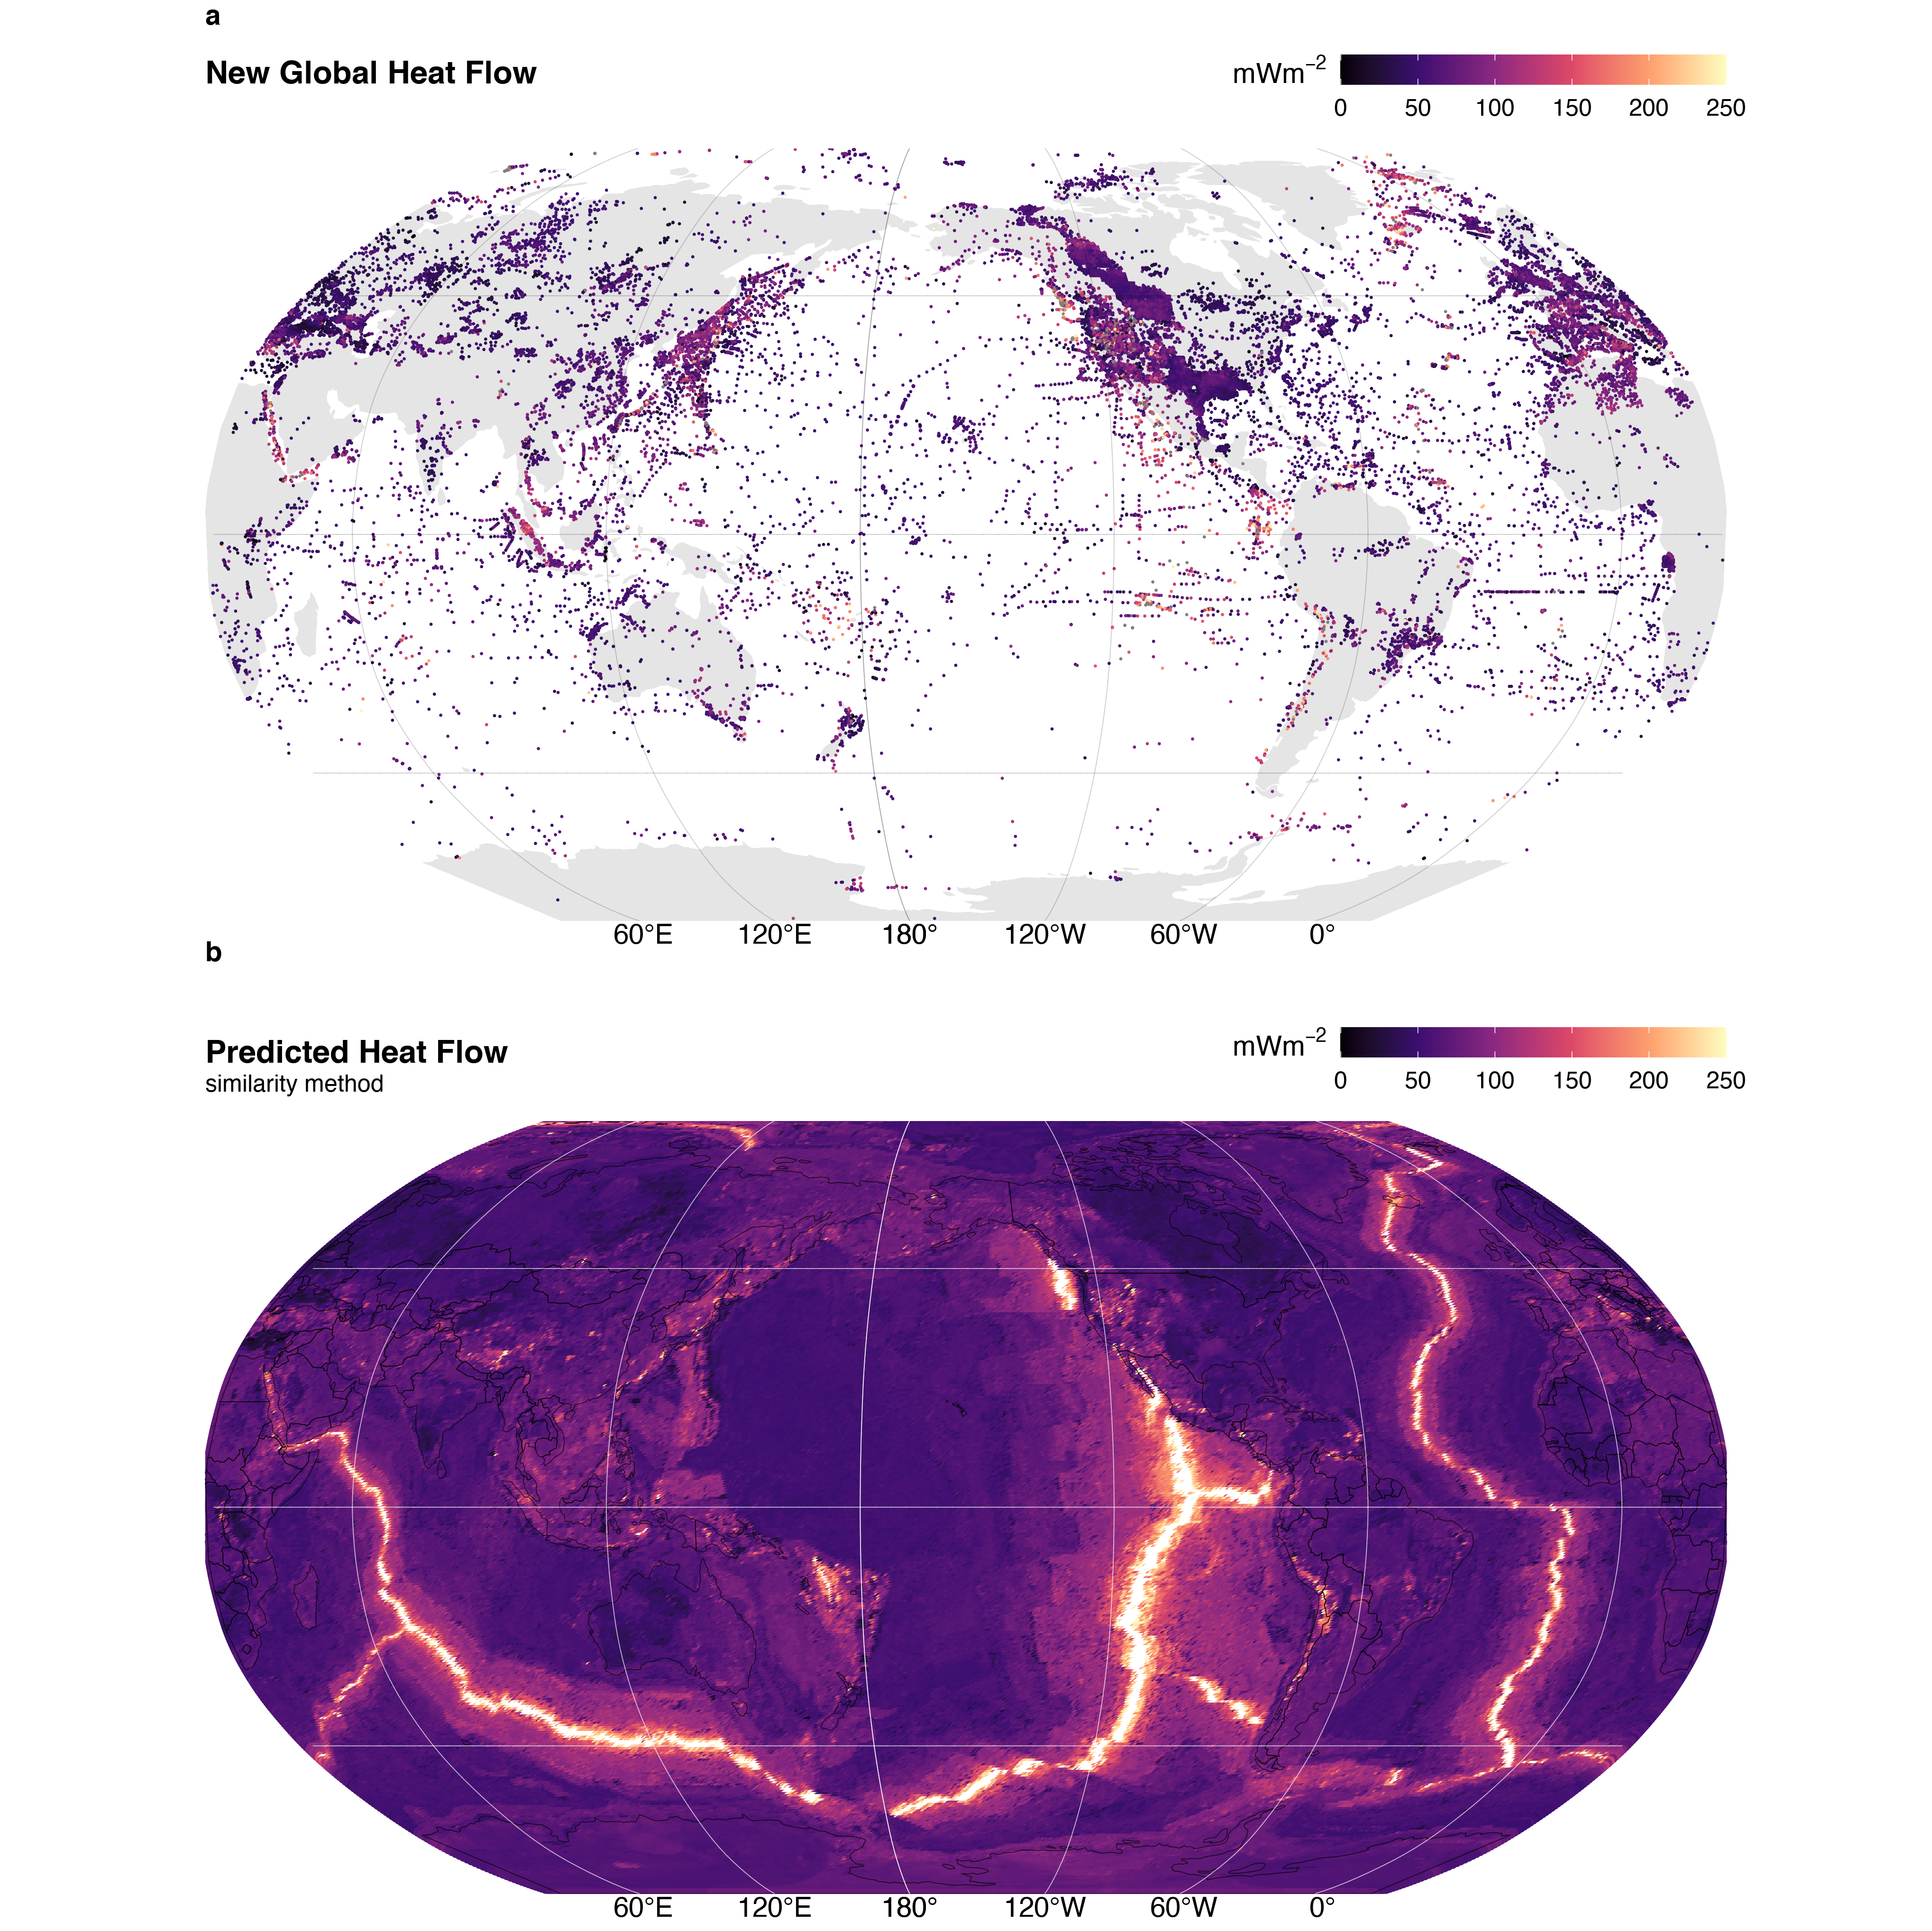
\includegraphics[width=0.95\linewidth,]{../figs/base/hf_luca} 

}

\caption{Global heat flow. (a) The NGHF database (n = 69729) and (b) interpolation by similarity method. Data from Lucazeau (2019).}\label{fig:lucahf}
\end{figure}

In contrast to the Third Law, there exists some degree of spatial
dependence, or continuity, in the distribution of surface heat flow. A
pair of surface heat flow observations taken one meter apart will be
strongly correlated. The correlation between pairs of observations will
likely decrease with increasing distance between the pairs (Goovaerts,
1997). This is encapsulated in the First Law of Geography (hereafter
referred to as the First Law): \emph{everything is related, but nearer
things are more related} (Krige, 1951; Matheron, 1963). The spatial
(dis)continuity of surface heat flow represents the areal extent of
geodynamic processes and their interactions. For example, patterns of
consistently low surface heat flow outline the areal extent of cratons
(Figure~\ref{fig:lucahf}) and consistent patterns of heat flow near
volcanic arcs are interpreted to reflect common backarc lithospheric
thermal structures (Currie et al., 2004; Currie \& Hyndman, 2006; Roy D.
Hyndman et al., 2005) and slab-mantle mechanical coupling depths in
subduction zones (Yoshitsugu Furukawa, 1993; Kerswell et al., 2020; Wada
\& Wang, 2009).

Predicting surface heat flow by considering many nearby observations
(i.e.~Kriging, Krige, 1951) is advantageous because spatial dependence
is conserved and uncertainty is only dependent on the distance between
pairs of observations (Chiles \& Delfiner, 2009). However, Kriging is
disadvantageous because it assumes that the underlying distribution of
heat flow is \emph{stationary} (constant in space and time), which
likely fails in geodynamically complex regions. This problem is overcome
by relaxing assumptions of stationarity and applying techniques that
respect the Second Law of Geography: \emph{spatial phenomena are
inherently heterogenous} (Goodchild, 2004), such as directional Kriging
or Markov-Bayes techniques that include proxies as priors (Bárdossy,
1997).

In this study we attempt to answer the following questions: 1) Are
global heat flow interpolations predicted by Kriging and similarity
methods comparable? 2) What are the implications of the differences
according to the implicit assumptions embodied in the First and Third
Laws of Geography? 3) Which method is better suited for hypothesis
testing? 4) How can the interpolations presented here guide future data
collection efforts?

We first use ordinary Kriging to interpolate the New Global Heat Flow
(NGHF) database of F. Lucazeau (2019). We then compare our interpolation
results to those of F. Lucazeau (2019) and consider the implications of
Kriging (First Law) vs.~similarity (Third Law) methods of interpolation.
We restrict our comparison to areas near subduction zone segments
defined by Syracuse \& Abers (2006) for two reasons: 1) to provide heat
flow interpolations and statistics useful to subduction zone research,
and 2) to emphasize differences and idiosyncrasies in both interpolation
approaches in a complex tectonic and thermal setting. We find that
Kriging and similarity methods are comparable for most subduction
segments. Both interpolations show inconsistent patterns of heat flow
and spatial continuity. This result implies single trench-perpendicular
heat flow samples is an incomplete framework for hypothesis testing.
Further, inconsistent spatial continuity and heat flow patterns counter
hypotheses of common thermal structure and geodynamics among subduction
zones. We suggest future research focus on generating high-quality
interpolations and discuss considerations for data acquisition
priorities.

\section{Methods}

\subsection{The NGHF Database}

The NGHF database was downloaded from the supplementary material of F.
Lucazeau (2019). It contains 69729 data points, their locations in
latitude/longitude, and metadata---including a data quality rank (Code
6) from A to D (with Code 6 = Z = undetermined). The reader is referred
to F. Lucazeau (2019) for details on compilation, references, and
historical perspective on the NGHF and previous compilations. We use
NGFH because it is the most recent database available, has been
carefully compiled, and is open-access.

Like F. Lucazeau (2019), we exclude 4790 poor quality observations (Code
6 = D) from our analysis. We further remove 350 data points without heat
flow observations and two without geographic information. Multiple
observations at the same location are parsed to avoid singular
covariance matrices during Kriging:

\begin{equation}\protect\hypertarget{eq:parse}{}{\begin{aligned}
    f(X_i^q, Y_i^q) &= \\
    X_i^q > Y_i^q &\rightarrow z_i = x_i \\
    X_i^q < Y_i^q &\rightarrow z_i = y_i \\
    X_i^q = Y_i^q &\rightarrow z_i = RAND(x_i, y_i)
    \end{aligned}}\label{eq:parse}\end{equation}

where \(X_i^q\) and \(Y_i^q\) represent the quality of each duplicate
observation pair at location \(i\), \(RAND\) is a random function that
selects either the observation \(x_i\) or \(y_i\), and \(z_i\) stores
the observation selected by \(f(X_i^q, Y_i^q)\). The final dataset used
for Kriging has \(n=\) 55274 observations after parsing \(n=\) 32430
duplicate observation.

\subsection{Kriging}

Kriging is a three-step process that involves first estimating an
experimental variogram, \(\hat{\gamma}(h)\), fitting the experimental
variogram with one of many variogram models, \(\gamma(h)\), and finally
using the modelled variogram to predict random variables at unknown
locations (Cressie, 2015; Krige, 1951). We use the general-purpose
functions defined in the ``R'' package \texttt{gstat} (Gräler et al.,
2016; Pebesma, 2004) to perform all three steps. We begin by estimating
an experimental variogram as defined by Bárdossy (1997):

\begin{equation}\protect\hypertarget{eq:variogram}{}{\hat{\gamma}(h) = \frac{1}{2N(h)}\sum_{N(h)}^{}(Z(u_i) - Z(u_j))^2}\label{eq:variogram}\end{equation}

where \(N(h)\) is the number of pairs of points, \(Z(u_i)\) and
\(Z(u_j)\), separated by a lag distance, \(h = |u_i - u_j|\). We
evaluate \(\hat{\gamma}(h)\) at fifteen lag distances by binning the
irregular spaced data with a bin width, \(\delta\), equal to a
proportion of the maximum lag distance, \(c\), divided by the number of
lags used to evaluate the variogram. The lag cutoff parameter, \(c\), is
optimized by genetic algorithm (discussed below). The binwidth is then
\(\delta = \max (N(h))/(15c)\), and
\(N(h) \leftarrow N(h, \delta h) = \{i,j:|u_i - u_j| \in [h - \delta h, h + \delta h)\}\).
In simple terms, Equation~\ref{eq:variogram} represents the similarity,
or dissimilarity, between pairs of observations in space.
Equation~\ref{eq:variogram} is adheres to the First Law of Geography and
is derived from the theory of \emph{regionalized variables} (Matheron,
1963, 2019), which formally defines a probabilistic framework for
spatial interpolation of natural phenomena. It is important for the
reader to understand the fundamental assumptions implicit in
Equation~\ref{eq:variogram} in order to understand the comparison of
interpolation techniques discussed later. The basic assumptions used in
our Kriging method are:

\begin{itemize}
\item
  \(\hat{\gamma}(h)\) is directionally invariant (isotropic)
\item
  \(\hat{\gamma}(h)\) is evaluated in two-dimensions and neglects
  elevation, \(Z(u) \in \mathbb{R}^2\)
\item
  The first and second moments of \(Z(u)\) have the following conditions
  over the domain \(D\):

  \begin{equation}\protect\hypertarget{eq:assumptions}{}{\begin{aligned}
        &E[Z(u)] = mean = constant, &\forall u \in D \\
        &E[(Z(u + h) - mean)(Z(u) - mean)] = C(h), &\forall |u, u + h| \in D
        \end{aligned}}\label{eq:assumptions}\end{equation}
\end{itemize}

The last assumption (Equation~\ref{eq:assumptions}) is called
``second-order stationarity'' and is implicit in the First Law of
Geography. It assumes the underlying probability distribution of the
random variable, \(Z(u)\), does not change in space and the covariance,
\(C(h)\), only depends on the distance, \(h\), between two random
variables. These assumptions are expected to be valid in cases where the
underlying natural process is stochastic, spatially continuous, and has
the property of additivity such that \(\frac{1}{n}\sum_{i=1}^n Z(u_i)\)
has the same meaning as \(Z(u)\) (Bárdossy, 1997).

The following are two illustrative cases where
Equation~\ref{eq:assumptions} is likely valid:

\begin{enumerate}
\def\labelenumi{\arabic{enumi}.}
\item
  The thickness of a sedimentary unit with a homogeneous concentration
  of radioactive elements can be approximated by
  \(q_s = q_b + \int A \,dz\), where \(q_b\) is a constant heat flux
  entering the bottom of the layer and \(A\) is the heat production
  within the layer with thickness \(z\) (Furlong \& Chapman, 2013). If
  we have two samples, \(Z(u_1) = 31~mW/m^2\) and
  \(Z(u_2) = 30.5~mW/m^2\), their corresponding thicknesses would be
  \(Z'(u_1) = 1000~m\) and \(Z'(u_2) = 500~m\) for \(A = 0.001~mW/m^3\)
  and \(q_b = 30~mW/m^2\). The variable, \(Z(u)\), in this case is
  additive because the arithmetic mean of the samples is a good
  approximation of the average sedimentary layer thickness,
  \((Z(u_1) + Z(u_2)) / 2 = 750~m\).
\item
  The age of young oceanic lithosphere can be approximated by
  \(q_s(t) = kT_b(\pi\kappa t)^{-1/2}\), where \(q_s(t)\) is the surface
  heat flow of a plate with age, \(t\), \(T_b\) is the temperature at
  the base of the plate, \(k\) is thermal conductivity, and
  \(\kappa = k/\rho C_p\) is thermal diffusivity (Carol A. Stein \&
  Stein, 1992). For \(k = 3.138~W/mK\), \(\rho = 3330~kg/m^3\),
  \(C_p = 1171~J/kgK\), \(T_b = 1350^{\circ}C\), two samples,
  \(Z(u_1) = 180~mW/m^2\) and \(Z(u_2) = 190~mW/m^2\), would correspond
  to plates with ages of \(Z'(u_1) = 10~Ma\), and \(Z'(u_2) = 9~Ma\),
  respectively. Since \(Z(u_1) + Z(u_2) / 2 = 185~mW/m^2\) and
  \(Z'(185~mW/m^2) = 9.5~Ma = Z'(u_1) + Z'(u_2) / 2\), the variable
  \(Z(u)\) in this case is also additive.
\end{enumerate}

In contrast, Equation~\ref{eq:assumptions} is likely invalid in regions
that transition among two or more tectonic regimes. For example, the
expected heat flow \(E[Z(u)] = mean\) will change when moving from a
spreading center to a subduction zone. \(E[Z(u)] = mean \neq constant\)
over the region of interest. Proceeding with
Equation~\ref{eq:assumptions} in this case has the effect of masking the
geodynamic complexity. In other words, the First Law of Geography is
violated and the geodynamic complexity will be \emph{invisible} to
Kriging predictions unless heatflow observations are sufficiently dense.
We will see that this has important implications when comparing our
Kriging method to F. Lucazeau (2019)'s interpolation method, which is
exactly opposite of this formalism---it only considers the similarities
among physical proxies and not spatial dependence.

The second step is to fit the experimental variogram with a variogram
model, \(\gamma(h)\). In this study we fit two popular variogram models
to the experimental variogram. We use models with sills, which implies
the spatial dependence between pairs of points has a finite range. The
spherical and exponential variogram models used in this study are
defined as (Chiles \& Delfiner, 2009; Cressie, 2015):

\begin{equation}\protect\hypertarget{eq:varmodels}{}{
\begin{aligned}
    sph &\leftarrow \gamma(h) =
        \begin{cases}
            n + s \left(\frac{3h}{2a} - \frac{1}{2}\left(\frac{h}{a}\right)^3\right), & \text{if } 0 \leq h \leq a \\
            n + s, & \text{if } h > a
        \end{cases} \\
    exp &\leftarrow \gamma(h) = n + s \left(1 - exp\left(\frac{-h}{a}\right)\right), ~\quad\text{if } h \geq 0 \\
\end{aligned}
}\label{eq:varmodels}\end{equation}

where \(n\) is the nugget, \(s\) is the sill, and \(a\) is the effective
range. The effective range, \(a\), is related to the range, \(r\), by
\(a = r\) and \(a = r/3\) for spherical and exponential models,
respectively (Gräler et al., 2016; Pebesma, 2004). We use the function
\texttt{fit.variogram} in \texttt{gstat} to try both variogram models.
The best model is selected by the minimum misfit by weighted least
square (WLS, Pebesma, 2004).

We use ordinary Kriging for our interpolation step, which predicts the
value of a random function, \(\hat{Z}(u)\), at unknown locations as a
linear combination of all known locations in the domain, \(D\)
(Bárdossy, 1997):

\begin{equation}\protect\hypertarget{eq:linestimate}{}{ \hat{Z}(u) = \sum_{i=1}^n \lambda_i Z(u_i), \quad \forall u \in D }\label{eq:linestimate}\end{equation}

The conditions in Equation~\ref{eq:assumptions} set up a constrained
minimization problem since one has:

\begin{equation}\protect\hypertarget{eq:firstmoment}{}{ E[Z(u)] = mean, \quad \forall u \in D }\label{eq:firstmoment}\end{equation}

The linear estimator must obey

\begin{equation}\protect\hypertarget{eq:explinestimate}{}{ E[\hat{Z}(u)] = \sum_{i=1}^n \lambda_i E[Z(u_i)] = mean }\label{eq:explinestimate}\end{equation}

so the weights must be

\begin{equation}\protect\hypertarget{eq:unbiased}{}{ \sum_{i=1}^n \lambda_i = 1 }\label{eq:unbiased}\end{equation}

This is the first constraint, also known as the unbiased condition,
which states that the sum of the weights must equal one. However, there
is an infinite set of real numbers one could use for the weights,
\(\lambda_i\). Our goal is to find the set of weights in
Equation~\ref{eq:linestimate} that minimizes the estimation variance.
This can be solved by minimizing the covariance function, \(C(h)\) from
Equation~\ref{eq:assumptions}:

\begin{equation}\protect\hypertarget{eq:minvar}{}{
\begin{aligned}
    \sigma^2(u) = Var[Z(u) - \hat{Z}(u)] = E\left[(Z(u) - \sum_{i=1}^n \lambda_i Z(u_i))^2\right] &= \\
    E\left[Z(u)^2 + \sum_{j=1}^n \sum_{i=1}^n \lambda_j \lambda_i Z(u_j)Z(u_i) - 2 \sum_{i=1}^n \lambda_i Z(u_i)Z(u)\right] &= \\
    C(0) + \sum_{j=1}^n \sum_{i=1}^n \lambda_j \lambda_i C(u_i - u_j) - 2 \sum_{i=1}^n \lambda_i C(u_i - u)
\end{aligned}
}\label{eq:minvar}\end{equation}

Minimizing Equation~\ref{eq:minvar} with respect to the unbiased
condition (Equation~\ref{eq:unbiased}), yields the best linear unbiased
estimator (BLUE, Bárdossy, 1997) for Equation~\ref{eq:linestimate} and
together are considered the Kriging system. In our case, this is done by
the function \texttt{krige} in \texttt{gstat}. We use the function
\texttt{krige.cv} in \texttt{gstat} to estimate the misfit between
observations and Kriging interpolations by ten-fold cross validation
(Pebesma, 2004).

Further, we use a general purpose genetic algorithm, \texttt{ga}, from
the R package, \texttt{GA} (Scrucca, 2013, 2017), to optimize Kriging
parameters after Z. Li et al. (2018). The results from the genetic
algorithm are comparable to the non-genetic-algorithm results. However,
some inconsistent variogram fitting by the algorithm is suspect. We
present these results and discuss their implications in
sec.~\ref{sec:ga}.

\subsection{Map Projection and Interpolation Grid}

We interpolate onto the same 0.5\(^{\circ}\)C x 0.5\(^{\circ}\)C grid as
F. Lucazeau (2019) so a direct difference could be calculated between
our interpolation methods and F. Lucazeau (2019)'s. The NGHF and grid
with predicted heat flow from F. Lucazeau (2019) were transformed into a
Pacific-centered Robinson coordinate reference system (CRS) defined
using the \texttt{proj} string (PROJ contributors, 2021):

\begin{verbatim}
+proj=robin +lon_0=-155 +lon_wrap=-155 +x_0=0 +y_0=0
+ellps=WGS84 +datum=WGS84 +units=m +no_defs
\end{verbatim}

All geographic operations, including Kriging and taking the difference
with F. Lucazeau (2019)'s heat flow predictions, are performed in the
above CRS using the general-purpose functions in the ``R'' package
\texttt{sf} (Pebesma, 2018). We define the Kriging domain near
individual arc segments in two steps: 1) 1000 \(km\) buffers are drawn
around the arc segments as defined by Syracuse \& Abers (2006). 2) The
bounding box of the 1000 \(km\) buffer is expanded by 10\% on all sides
(Figure~\ref{fig:segments}). We use F. Lucazeau (2019)'s grid for
Kriging predictions so differences can be taken point-by-point at the
exact same locations.

We provide the complete NGHF database (F. Lucazeau, 2019), filtered and
parsed NGHF database, heat flow interpolations (from F. Lucazeau, 2019,
and this study), and our code as supplementary information to support
FAIR data policy (Wilkinson et al., 2016). These materials can also be
retrieved from the official repository at
\url{https://doi.org/10.17605/OSF.IO/CA6ZU}.

\begin{figure}[h]

{\centering \includegraphics[width=0.95\linewidth,]{../figs/base/segs_comp} 

}

\caption{Subduction zone segments and interpolation domain. (a) Heat flow is interpolated around thirteen subduction zone segments by (b) drawing a 1000km buffer (lightest blue) around each segment and expanding the buffer's bounding box (medium blue) by 10\% on all sides (darkest blue). (c) The NGHF database is cropped within the largest rectangle. Data from Syracuse \& Abers (2006) and Lucazeau (2019).}\label{fig:segments}
\end{figure}

\clearpage

\section{Results}

\subsection{Heat Flow Near Subduction Zone Segments}

Summary statistics for surface heat flow observations by subduction zone
segment are given in Table~\ref{tbl:hf.summary.table} and
Figure~\ref{fig:hf.summary.plot}. Surface heat flow is median-centered
around 45-70 \(mWm^{-2}\) and narrowly distributed (excluding outliers)
with inter-quartile ranges (IQR) from 12 to 50 \(mWm^{-2}\) for most
subduction zone segments. Alaska Aleutians is the exception with a
higher median of 184 \(mWm^{-2}\) and broader range (IQR =
\(250~mW^{-2}\)). The whole distributions (including outliers) for all
segments are strongly right-skewed with maximum heat flow values of
several thousand of \(mWm^{-2}\) or more. Heat flow values above 250
\(mWm^{-2}\) are considered geothermal areas by F. Lucazeau (2019),
which we adopt as a relevant empirical limit for anomalously high heat
flow.

\hypertarget{tbl:hf.summary.table}{}
\begin{longtable}[]{@{}lrrrrrrr@{}}
\caption{\label{tbl:hf.summary.table}Heat flow (\(mWm^{-2}\))
observations}\tabularnewline
\toprule
Segment & n & Min & Max & Median & IQR & Mean & Sigma \\
\midrule
\endfirsthead
\toprule
Segment & n & Min & Max & Median & IQR & Mean & Sigma \\
\midrule
\endhead
Alaska Aleutians & 2793 & 4 & 7765 & 183 & 206 & 232 & 344 \\
Andes & 5227 & 7 & 911 & 45 & 50 & 87 & 88 \\
Central America & 5042 & 8 & 911 & 45 & 48 & 88 & 90 \\
Kamchatka Marianas & 3957 & 1 & 21700 & 71 & 48 & 118 & 548 \\
Kyushu Ryukyu & 3244 & 1 & 21700 & 72 & 44 & 127 & 604 \\
Lesser Antilles & 3535 & 13 & 1334 & 41 & 12 & 52 & 54 \\
N Philippines & 1002 & 3 & 21700 & 71 & 35 & 194 & 1051 \\
New Britain Solomon & 181 & 3 & 174 & 66 & 43 & 69 & 30 \\
S Philippines & 1444 & 1 & 21700 & 71 & 43 & 158 & 874 \\
Scotia & 72 & 13 & 145 & 76 & 23 & 74 & 28 \\
Sumatra Banda Sea & 3040 & 1 & 5600 & 65 & 47 & 77 & 120 \\
Tonga New Zealand & 506 & 2 & 416 & 54 & 40 & 64 & 45 \\
Vanuatu & 349 & 2 & 283 & 54 & 40 & 64 & 44 \\
\bottomrule
\end{longtable}

\begin{figure}[h]

{\centering \includegraphics[width=0.6\linewidth,]{../figs/summary/hf_summary} 

}

\caption{Distribution of heat flow observations. Heat flow near most segments is centered around $50~mWm^{-2}$ and highly skewed right (shadowy dot outliers). The skeweness likely represents sampling near geothermal systems, volcanic arcs, or spreading centers. Data from Lucazeau (2019).}\label{fig:hf.summary.plot}
\end{figure}

\subsection{Variogram Models}

The optimal variogram models and associated errors \(C_F(\Theta)\) and
\(C_I(\Theta)\) are given in Table~\ref{tbl:variogram.summary.table}.
Almost twice as many experimental variograms are fit with spherical
models (8) compared to exponential models (5). Variogram model sills
vary substantially among the subduction zone segments between 9 and 1538
\(mWm^{-2}\). Variogram model ranges also vary substantially among
segments from 4 to 1676 \(km\).

No apparent correlation exists between variogram model range and
subduction zone segment length, number of heat flow observations, nor
domain area (Figure~\ref{fig:variogram.summary.plot}). Most subduction
zone segments show spatial dependence of a few hundred kilometers or
less, irrespective of the number of observations or segment size. The
exceptions are Kyushu Ryukyu (range = 1774 \(km\)) and Vanuatu (range =
573 \(km\)), whose model variogram ranges are, perhaps, anomalously
high.

\hypertarget{tbl:variogram.summary.table}{}
\begin{longtable}[]{@{}llrr@{}}
\caption{\label{tbl:variogram.summary.table}Optimal varigram
models}\tabularnewline
\toprule
Segment & Model & Sill \([mWm^{-2}]\) & Range \([km]\) \\
\midrule
\endfirsthead
\toprule
Segment & Model & Sill \([mWm^{-2}]\) & Range \([km]\) \\
\midrule
\endhead
Alaska Aleutians & Sph & 284 & 222 \\
Andes & Sph & 87 & 341 \\
Central America & Sph & 85 & 336 \\
Kamchatka Marianas & Exp & 580 & 277 \\
Kyushu Ryukyu & Exp & 802 & 864 \\
Lesser Antilles & Exp & 36 & 80 \\
N Philippines & Sph & 1118 & 240 \\
New Britain Solomon & Exp & 29 & 85 \\
S Philippines & Sph & 956 & 413 \\
Scotia & Exp & 9 & 4 \\
Sumatra Banda Sea & Exp & 113 & 32 \\
Tonga New Zealand & Sph & 47 & 129 \\
Vanuatu & Sph & 48 & 573 \\
\bottomrule
\end{longtable}

\begin{figure}[h]

{\centering \includegraphics[width=0.95\linewidth,]{../figs/summary/variogram_summary} 

}

\caption{Summary of variogram model ranges and correlations with other features. (a) Variogram model ranges are variable, but generally below 400 km. Variogram model ranges show no correlation with segment length (b), number of heat flow observations (c), nor domain area (d). The spatial dependenc of heat flow is apparently independent of these parameters.}\label{fig:variogram.summary.plot}
\end{figure}

\subsection{Interpolation Comparison}

Summary statistics for the interpolation differences are given in
Table~\ref{tbl:diff.summary.table} and
Figure~\ref{fig:diff.summary.plot}. Note that the difference is taken at
the exact same locations for every prediction. Differences between the
similarity method and Kriging are small for most segments with the
exception of Central America, which shows a broader distribution of
differences than the other segments. The median differences range from
-9 to 7 \(mWm^{-2}\) with inter quartile ranges from 15 to 62
\(mWm^{-2}\). Similar to the distribution of heat flow in these areas,
the minimum and maximum difference in predicted heat flow are extreme
and represent the failure of one method to predict extreme outliers of
the other.

\hypertarget{tbl:diff.summary.table}{}
\begin{longtable}[]{@{}lrrrrrr@{}}
\caption{\label{tbl:diff.summary.table}Predicted heat flow
(\(mWm^{-2}\)) differences}\tabularnewline
\toprule
Segment & Min & Max & Median & IQR & Mean & Sigma \\
\midrule
\endfirsthead
\toprule
Segment & Min & Max & Median & IQR & Mean & Sigma \\
\midrule
\endhead
Alaska Aleutians & -551 & 2633 & -2 & 20 & 3 & 71 \\
Andes & -240 & 2336 & 2 & 35 & 13 & 72 \\
Central America & -241 & 2731 & 8 & 63 & 43 & 147 \\
Kamchatka Marianas & -2491 & 297 & 4 & 15 & 4 & 39 \\
Kyushu Ryukyu & -2492 & 143 & 6 & 21 & 2 & 74 \\
Lesser Antilles & -99 & 589 & 0 & 16 & 6 & 32 \\
N Philippines & -2136 & 284 & 2 & 24 & 0 & 65 \\
New Britain Solomon & -80 & 237 & 1 & 22 & 5 & 20 \\
S Philippines & -272 & 370 & 5 & 26 & 7 & 30 \\
Scotia & -62 & 1001 & -4 & 24 & 5 & 33 \\
Sumatra Banda Sea & -243 & 385 & -2 & 20 & 1 & 19 \\
Tonga New Zealand & -113 & 1696 & -9 & 23 & -2 & 30 \\
Vanuatu & -166 & 1657 & 7 & 27 & 8 & 40 \\
\bottomrule
\end{longtable}

Prediction differences are either approximately normally distributed, or
skewed right. Right skew and a tendency of medians to deviate positively
from zero both reflect a systematic overprediction of heat flow by the
similarity method compared to Kriging
(Figure~\ref{fig:diff.summary.plot}). However, Alaska Aleutians, Scotia,
and Tonga New Zealand have negative median differences. While there is a
tendency for the similarity method to overpredict heat flow compared to
Kriging, it is not true in every case.

\begin{figure}[h]

{\centering \includegraphics[width=0.6\linewidth,]{../figs/summary/hf_diff_summary} 

}

\caption{Point-by-point differences of predicted heat flow between similarity and Kriging interpolations. The differences for most subduction zone segments are median-centered at or near-zero with IQRs from 16 to 62. Outliers (shadowy dots) extend to extreme positive and negative differences.}\label{fig:diff.summary.plot}
\end{figure}

Notable sources of prediction differences include 1) tectonic features
predicted by similarity that are absent from Kriging or 2) general
discordance between the spatial continuity of heat flow observations and
similarity predictions. For example, high heat flow representing
Galápagos triple junction is predicted by similarity to the SW of the
Central America segment (Figure~\ref{fig:central.america.diff} a).
However, none of the triple junction arms, nor the Galápagos hot spot,
are well defined in the Kriged prediction
(Figure~\ref{fig:central.america.diff} b). The interpolation comparison
for Central America highlights two distinct regions---bright differences
along the arms of the triple junction and muted agreement to the E and
NE of the Cocos Plate (Figure~\ref{fig:central.america.diff} c). Note
the moderate differences within the Cocos Plate in
Figure~\ref{fig:central.america.diff} a where similarity predicts high
heat flow by proximity to the nearby spreading centers, but heat flow in
the region is, in fact, relatively low (compare
Figure~\ref{fig:central.america.diff} a, b, c). Similar discordance
between high similarity predictions and low heat flow observations are
observed in many subduction zone segments, especially near spreading
centers predicted by similarity (e.g. Figure~\ref{fig:andes.comp}; see
sec.~\ref{sec:comps}).

\begin{figure}[h]

{\centering \includegraphics[width=0.95\linewidth,]{../figs/diff/custom/Central_America} 

}

\caption{Similarity vs. Kriging predictions for Central America. The Galápagos triple junction (GTJ), East Pacific Rise (EPR), and Cocos Ridge (CR) are predicted by similarity (a), but not by Kriging (b). Note the moderate difference between predictions within the Cocos Plate (CP) where similarity predicts high heat flow but observations are low (c). Bold and thin white lines represent the subduction zone segment boundary and plate depth, respectively, as defined by Syracuse \& Abers (2006). Heat flow data and similarity prediction from Lucazeau (2019).}\label{fig:central.america.diff}
\end{figure}

On the other side of the Caribbean Plate, near the Lesser Antilles
segment, similarity and Kriging predictions show good agreement. The
Mid-Atlantic Ridge to the E appears in both predictions
(Figure~\ref{fig:lesser.antilles.diff} a, b). The spreading center is
better defined with Kriging in this case, as compared to the Galápagos
triple junction, because the observational density and spatial coverage
near the Lesser Antilles segment are sufficiently high and continuous
near the Mid-Atlantic Ridge (see sec.~\ref{sec:comps}). However, the
comparison still highlight spreading centers as similarity tends to
predict higher heat flow than observations.

\begin{figure}[h]

{\centering \includegraphics[width=0.95\linewidth,]{../figs/diff/custom/Lesser_Antilles} 

}

\caption{Similarity vs. Kriging predictions for the Lesser Antilles. The Mid-Atlantic Ridge (MAR) predicted by similarity (a) is also defined by Kriging (b) because of adequate observational density and spatial coverage near the spreading center. Good agreement between similarity and Kriging exist for the entire domain (c). CBP = Caribbean Plate, SA = South America. Bold and thin white lines represent the subduction zone segment boundary and plate depth, respectively, as defined by Syracuse \& Abers (2006). Heat flow data and similarity prediction from Lucazeau (2019).}\label{fig:lesser.antilles.diff}
\end{figure}

Another example of good agreement between similarity and Kriging are
interpolations near the Sumatra Banda Sea segment
(Figure~\ref{fig:sumatra.banda.sea.diff};
Figure~\ref{fig:sumatra.banda.sea.comp}). Note the textural and
structural complexity predicted by similarity
(Figure~\ref{fig:sumatra.banda.sea.diff} a) compared to the smooth
featureless Kriging predictions (Figure~\ref{fig:sumatra.banda.sea.diff}
b). Despite the textural and structural differences, the difference
between similarity and Kriging within the Sunda Plate, Australian Plate,
and W Philippine Sea Plate is small
(Figure~\ref{fig:sumatra.banda.sea.diff} c).

\begin{figure}[h]

{\centering \includegraphics[width=0.95\linewidth,]{../figs/diff/custom/Sumatra_Banda_Sea} 

}

\caption{Similarity vs. Kriging predictions for Sumatra Banda Sea. Similarity predictions are texutrally and structurally complex (a), while Kriging is smooth and featureless (b). Despite the textural and structural difference, the interpolations are similar, especially within the Sunda Plate (SNP), Australian Plate (AUP) and W Philippine Sea Plate (PSP). Bold and thin white lines represent the subduction zone segment boundary and plate depth, respectively, as defined by Syracuse \& Abers (2006). Heat flow data and similarity prediction from Lucazeau (2019).}\label{fig:sumatra.banda.sea.diff}
\end{figure}

Heat flow predictions near the Scotia segment illustrate a case where
heat flow observations are incredibly sparse. Similarity predicts high
heat flow from the East Scotia Ridge (ESR) and the WSW-ENE trending
transform boundary separating the Scotia and Sandwich Plates from the
Antartic Plate (Figure~\ref{fig:scotia.diff} a).
Figure~\ref{fig:scotia.diff} b appears featureless because very few heat
flow observations (n = 72) define a flat experimental variogram for all
lag distances greater than four kilometers (no spatial dependence beyond
4 km, Table~\ref{tbl:variogram.summary.table};
Figure~\ref{fig:scotia.comp}). Kriging predicts the expected (mean) heat
flow value for the entire domain (Figure~\ref{fig:scotia.diff} b), in
this case, according to Equation~\ref{eq:linestimate}. Interestingly,
the expected heat flow is a fine predictor for most of the ocean basin,
except near the spreading center and transform fault
(Figure~\ref{fig:scotia.diff} c). The New Britain Solomon segment shows
a similar comparison (Figure~\ref{fig:new.britain.solomon.comp}) with
good agreement between similarity and Kriging despite very few heat flow
observations, little spatial dependence (small variogram range), and a
featureless Kriged interpolation.

\begin{figure}[h]

{\centering \includegraphics[width=0.95\linewidth,]{../figs/diff/custom/Scotia} 

}

\caption{Similarity vs. Kriging predictions for Scotia. (a) Similarity predicts high heat flow for two tectonic features, the East Scotia Ridge (ESR) and a transform fault (TF) separating the Scotia and Sandwich Plates (SP, SAN) from the Antartic Plate (AP). Kriging (b) is featureless because of incredibly sparse data. Despite few heat flow observations. Kriging predictions are only significantly different than similarity predictions near the ESR and transform fault (c). Bold and thin white lines represent the subduction zone segment boundary and plate depth, respectively, as defined by Syracuse \& Abers (2006). Heat flow data and similarity prediction from Lucazeau (2019).}\label{fig:scotia.diff}
\end{figure}

While similarity tends to define tectonic features and Kriging tends to
smooth out tectonic features, we find the opposite pattern within the
tectonically-complex region near Vanuatu. Similarity predicts the N-S
trending spreading center separating the New Hebrides plate from the
Balmoral Reef and Conway Reef microplates (Figure~\ref{fig:vanuatu.diff}
a). However, heat flow observations are sufficiently dense and
continuous to partially resolve the short ridge segments and transform
faults outlining the microplates between Vanuatu and the Tonga New
Zealand segments by Kriging (Figure~\ref{fig:vanuatu.diff} b). The
differences (Figure~\ref{fig:vanuatu.diff} c) are difficult to interpret
because of the somewhat random discordance between interpolation
methods.

\begin{figure}[h]

{\centering \includegraphics[width=0.95\linewidth,]{../figs/diff/custom/Vanuatu} 

}

\caption{Similarity vs. Kriging predictions for Vanuatu. (a) Similarity resolved the spreading center separating the New Hebrides Plate (NHP) from the Balmoral Reef (BR) and Conway Reef (CR) microplates. Sufficient heat flow observations allow Kriging to resolve additional ridge segments and transform faults outlining BR and CR (b). The difference between similarity and Kriging (c) is discordant and difficult to interpret. Bold and thin white lines represent the subduction zone segment boundary and plate depth, respectively, as defined by Syracuse \& Abers (2006). Heat flow data and similarity prediction from Lucazeau (2019).}\label{fig:vanuatu.diff}
\end{figure}

\clearpage

\section{Discussion}

\subsection{The First and Third Laws of Geography}

The Third Law of Geography states that \emph{two points with similar
geographic configurations should have similar values}. In the context of
heat flow near subduction systems and associated spreading centers, the
Third Law produces interpolations that highlight discrete tectonic
features (spreading centers and large fault systems) with complex
regional texture. At first glance the textural complexity may be
misconstrued as realistic interpolations, but is merely an artifact of
the similarity method. The texture predicted by similarity is artificial
insofar as it does not represent spatial changes in surface heat flow.
Rather each prediction location represents an independent assignment of
heat flow by association to all other locations with similar geographic
configurations (B. Goutorbe et al., 2011; F. Lucazeau, 2019; Zhu et al.,
2018). The extent to which similarity predictions represent real changes
of heat flow in space is entirely dependent on the reliability of the
Third Law, the quality of the physical proxies, and the selected
combination of proxies used for interpolation.

We note a few inconsistencies with F. Lucazeau (2019)'s similarity
predictions in the domains considered in this study. First, F. Lucazeau
(2019)'s predictions systematically overpredict heat flow near spreading
centers, justifying an adjustment to their algorithm. Second, known
tectonic features within the tectonically-complex region near Vanuatu
may be better resolved by Kriging than F. Lucazeau (2019)'s predictions.
It is important to note, however, that Vanuatu is the only case where
Kriging resolves tectonic features that similarity does not; the trend
is otherwise opposite. Moreover, the inconsistencies near Vanuatu do not
imply algorithmic issues and can likely be resolved by similarity using
a finer-scale grid.

The more important inconsistencies are general discordance between
similarity predictions and observations. Disagreements with observations
imply failures of the Third Law, which are not easily correctable
algorithmically. Cross-validation statistics given by F. Lucazeau (2019)
demonstrate good agreement with observations in general. The
cross-validation error may be sufficiently small for calculating global
heat flux and probing other relevant questions on the global scale.
However, testing hypotheses which require sampling heat flow on the
subduction zone segment scale should carefully consider where
predictions and observations differ, regardless of the interpolation
method (discussed further below).

Unlike the Third Law, the First Law of Geography by definition does not
allow discordance between predictions and observations. This fact can be
colloquially stated as \emph{everything is related, but nearer things
are more related (and points at the exact same location are perfectly
related)}. More formally, the covariance of two points at the same
location must be zero. Comparing the First and Third Laws reveals
further asymmetry in the sources of errors. Sources of interpolation
error include: 1) quality of heat flow observations (First \& Third
Law), 2) variance of predictions at unknown locations (First \& Third
Law), 3) residuals of predictions at known locations (Third Law), 4)
Kriging weights (variogram model; First Law), 5) variances of physical
proxies (Third Law), 6) combinations of physical proxies (Third Law), 7)
similarity weights (similarity model; Third Law). Interpolation
uncertainty is easier to conceptualize and quantify for First Law
interpolations than Third Law interpolations.

Arguments in favour of First or Third Law interpolations, however, are
not easily generalized. Third Law interpolations are justified in cases
with inadequate heat flow observations (e.g.~Scotia and New Britain
Solomon). First Law interpolations are arguably more favourable in all
cases with adequate heat flow observations because 1) enough
observations will resolve important features, 2) spatial dependency is
respected, and 3) there are fewer sources of uncertainty. However, it is
difficult to know what ``adequate'' observational density and spatial
coverage are \emph{a priori}. In any case, it may not be feasible to
achieve adequate observational density and spatial coverage due to time
and budget constraints. Therefore, hypotheses and sampling strategies
should be constructed with careful consideration of whether First or
Third Law interpolations are more appropriate on a case-by-case basis.

Regardless of the methodology, the present interpolations show
inconsistent patterns of heat flow and spatial variance, implying either
1) disorganized subsurface thermal structure, 2) spatially heterogeneous
dynamics, or 3) broad obfuscation of subsurface thermal structure and
dynamics by near-surface processes. Therefore we encourage a more
antireductionist view of subduction zone dynamics. We point out that
while testing of many important subduction-related questions may not be
feasible with the current global database, the idea of broad dynamic
commonality among subduction systems does not hold up to scrutiny from
the heat flow interpolations presented here.

\subsection{Hypothesis Testing}

Testing hypotheses relating to subduction dynamics require sampling of
heat flow in order to apply statistical models. Sampling in previous
work commonly uses a three-part strategy: 1) draw a cross-section line
perpendicular to the trench, 2) draw a rectangle with arbitrary width
bisected by the section line, 3) gather all heat flow observations
within the rectangle and project them onto the section line (e.g.,
Currie et al., 2004; Currie \& Hyndman, 2006; Roy D. Hyndman et al.,
2005; Wada \& Wang, 2009). This sampling strategy is simple and most
effective if measurements along section lines are equally spaced with
high spatial density. Observations along straight transects
perpendicular to trenches, however, are rare in the NGHF except for a
few studies e.g.~near the Lesser Antilles and Sumatra Banda Sea
segments, \ref{fig:NGHF}, (F. Lucazeau, 2019). There are additional
limitations to this method, including: 1) the method increasingly
violates the First Law as the size of the sampling rectangle
increases---projecting more disparate points onto the section line---and
2) sampling must be repeated many times along strike to fully
characterize the spatial distribution of heat flow near subduction zone
segments. Despite these limitations, previous work use single transects
to characterize whole subduction zones, which are then compared to make
broad claims about global subduction dynamics (e.g., Currie et al.,
2004; Currie \& Hyndman, 2006; Roy D. Hyndman et al., 2005; Kerswell et
al., 2020; Wada \& Wang, 2009).

Hypotheses such as common depths of slab-mantle mechanical coupling and
commonly thin backarc lithospheres (Currie et al., 2004; Currie \&
Hyndman, 2006; Yoshitsugu Furukawa, 1993; Kerswell et al., 2020; Wada \&
Wang, 2009) cannot be adequately tested using the single-transect method
described above. First and Third Law interpolations show that spatial
variance in heat flow near subduction zone segments is simply too high
to support any claim that subduction dynamics are operating on vastly
similar spatiotemporal scales either within or among subduction zone
segments. For example, sampling along section lines offset at 50 \(km\)
from previously published section lines (Currie et al., 2004; Currie \&
Hyndman, 2006; Yoshitsugu Furukawa, 1993; Wada \& Wang, 2009) is
unlikely to reproduce results. Insofar as heat flow can reliably answer
questions about subduction zone dynamics in space and time, hypothesis
must be qualified with sampling techniques that consider the appropriate
number of dimensions for the question being asked. Sampling and
projection onto a one-dimensional section line is insufficient for
testing hypotheses about the two-dimensional distribution of dynamic
processes.

\subsection{Heat Flow Sampling Strategies}

With a comparison of two approaches and interpolations, important
questions may be considered:

\begin{enumerate}
\def\labelenumi{\arabic{enumi}.}
\item
  Is collecting more heat flow data necessary for future subduction zone
  research?
\item
  Where should data collection efforts be focused?
\item
  Should First or Third Law interpolations be favoured when prioritizing
  data collection targets?
\end{enumerate}

More data collection is unequivocally conducive to deeper understanding
of subduction zone dynamics. Assuming inexpensive and rapid raster
acquisition of marine and terrestrial heat flow is far in the future,
discrete data collection from probes and boreholes remain the primary
methods of collection. Below we discuss reasonable strategies for data
collection without making concrete recommendations. We hope the reader
is convinced by now that two-dimensional interpolations of heat flow are
preferred for testing hypotheses regarding geodynamics near subduction
zones. Therefore, the focus of future data collection efforts should be
production of high-quality interpolations in these regions. Strategies
for producing higher-quality and higher-resolution interpolations
depends on the method, so a decision must first be made to use Kriging
(First Law), similarity (Third Law), or another method (e.g.~Second
Law).

Kriging interpolation quality scales with spatial density of
observations. High-density, grid-like surveys across the forearc and
backarc regions are likely to yield good results. Regularly-spaced grids
are preferred overs single transects because an infinite number of
transects can be sampled from a high-quality interpolation. Grid spacing
should not exceed the ranges given in
Table~\ref{tbl:variogram.summary.table}. Careful avoidance of potential
near-surface perturbations should be prioritized over regular spacing if
possible.

Surveying heat flow is temporally, energetically, and monetarily
expensive. We suggest prioritizing small segments like Scotia, the
Lesser Antilles, and New Britain Solomon as Kriging targets because they
currently have few observations and their relatively lengths allow for
denser surveying. An alternative strategy is to choose a segment with
existing high-density coverage and survey within observational gaps.
Regular spacing is less important in the latter case.

Similarity interpolation quality depends on the combination of physical
proxies and their associated heat flow distributions used in the
similarity algorithm (B. Goutorbe et al., 2011; F. Lucazeau, 2019).
Therefore, the quality of similarity interpolations scale with the
quality of the proxy datasets. A decision must first be made on the best
combination of proxy datasets, followed by careful scrutiny of the
quality of the dataset. B. Goutorbe et al. (2011) provides relevant
datasets with measures of each dataset's effect on a global heat flow
interpolation. Datasets with the strongest degradation effects (removing
them from the interpolation algorithm leads to less accurate results),
such as topography, lithospheric thickness, and velocity structure (B.
Goutorbe et al., 2011), should be used in future algorithms and
prioritized for quality control and improvement. The cost-benefit of
improving proxy datasets varies among datasets. Some datasets, like
topography, are relatively easy to improve through quality control and
remote acquisition, whereas improving other datasets, like lithospheric
heat production or lithospheric thickness, are more involved. Contending
with numerous datasets and sources of uncertainty (discussed above) make
improvements to Third Law interpolations challenging.

Simple Kriging methods are comparable to similarity methods for
interpolating heat flow near subduction zone systems according to
Figure~\ref{fig:diff.summary.plot} and
Table~\ref{tbl:diff.summary.table}. Improvements to Kriging
interpolations will likely outpace similarity methods with focused
surveying of specific segments because high-density surveying, although
costly, is more straightforward than simultaneously improving many proxy
datasets. Coincidentally, high-density sampling improves similarity
interpolations because any addition of high-quality measurements
incrementally improves existing proxy datasets. Therefore, we suggest
strategies for future heat flow acquisitions favour First Law
interpolations and focus on high-density surveying of one priority
segment at a time. In principle this strategy generates reliable First
Law interpolations while making incremental improvements to Third Law
interpolations.

\section{Conclusions}

This study uses Kriging to interpolate the New Global Heat Flow database
(F. Lucazeau, 2019) and makes a direct comparison between Kriging and
similarity (F. Lucazeau, 2019) interpolations near subduction zone
segments. The differences between interpolations highlight four
important points of consideration:

\begin{enumerate}
\def\labelenumi{\arabic{enumi}.}
\item
  Inconsistent patterns of heat flow and spatial variance characterize
  most subduction zone segments, countering hypotheses of common thermal
  structure or geodynamics (e.g.~coupling depths)
\item
  Kriging and similarity interpolation methods produce similar results
  near subduction zone segments
\item
  For testing hypotheses regarding thermal structure and geodynamics,
  sampling from two-dimensional interpolations is favoured over
  gathering and projecting discrete observations onto single-transects
\item
  Focused improvements to heat flow interpolations is encouraged to test
  current hypotheses and advance subduction zone research
\item
  Improving Kriging (First Law) interpolations through focused surveys
  within priority subduction zone segments is a favourable strategy for
  future data acquisition
\end{enumerate}

\section{Open Research}

All data, code, and heat flow interpolations can be found at
\texttt{https://doi.org/10.17605/OSF.IO/CA6ZU}, the official Open
Science Framework data repository. All code is MIT Licensed and free for
use and distribution (see license details).

\clearpage

\acknowledgments

We thank D. Hasterok for providing the NGHF references and guidance on
citing. This work was supported by the National Science Foundation grant
OIA1545903 to M. Kohn, S. Penniston-Dorland, and M. Feineman.

\section{References}

\hypertarget{refs_main}{}
\leavevmode\vadjust pre{\hypertarget{ref-bardossy1997}{}}%
Bárdossy, A. (1997). Introduction to geostatistics. \emph{Institute of
Hydraulic Engineering, University of Stuttgart}.

\leavevmode\vadjust pre{\hypertarget{ref-chapman1975}{}}%
Chapman, D. S., \& Pollack, H. N. (1975). Global heat flow: A new look.
\emph{Earth and Planetary Science Letters}, \emph{28}(1), 23--32.

\leavevmode\vadjust pre{\hypertarget{ref-chiles2009}{}}%
Chiles, J.-P., \& Delfiner, P. (2009). \emph{Geostatistics: Modeling
spatial uncertainty} (Vol. 497). John Wiley \& Sons.

\leavevmode\vadjust pre{\hypertarget{ref-cressie2015}{}}%
Cressie, N. (2015). \emph{Statistics for spatial data}. John Wiley \&
Sons.

\leavevmode\vadjust pre{\hypertarget{ref-currie2006}{}}%
Currie, C., \& Hyndman, R. D. (2006). The thermal structure of
subduction zone back arcs. \emph{Journal of Geophysical Research: Solid
Earth}, \emph{111}(B8).

\leavevmode\vadjust pre{\hypertarget{ref-currie2004}{}}%
Currie, C., Wang, K., Hyndman, R. D., \& He, J. (2004). The thermal
effects of steady-state slab-driven mantle flow above a subducting
plate: The cascadia subduction zone and backarc. \emph{Earth and
Planetary Science Letters}, \emph{223}(1-2), 35--48.

\leavevmode\vadjust pre{\hypertarget{ref-davies2013}{}}%
Davies, J. H. (2013). Global map of solid earth surface heat flow.
\emph{Geochemistry, Geophysics, Geosystems}, \emph{14}(10), 4608--4622.

\leavevmode\vadjust pre{\hypertarget{ref-fourier1827}{}}%
Fourier, J. (1827). M{é}moire sur les temp{é}ratures du globe terrestre
et des espaces plan{é}taires. \emph{M{é}moires de l'Acad{é}mie Royale
Des Sciences de l'Institut de France}, \emph{7}, 570--604.

\leavevmode\vadjust pre{\hypertarget{ref-furlong2013}{}}%
Furlong, K. P., \& Chapman, D. S. (2013). Heat flow, heat generation,
and the thermal state of the lithosphere. \emph{Annual Review of Earth
and Planetary Sciences}, \emph{41}, 385--410.

\leavevmode\vadjust pre{\hypertarget{ref-furukawa1993}{}}%
Furukawa, Y. (1993). Depth of the decoupling plate interface and thermal
structure under arcs. \emph{Journal of Geophysical Research: Solid
Earth}, \emph{98}(B11), 20005--20013.

\leavevmode\vadjust pre{\hypertarget{ref-gao2014}{}}%
Gao, X., \& Wang, K. (2014). Strength of stick-slip and creeping
subduction megathrusts from heat flow observations. \emph{Science},
\emph{345}(6200), 1038--1041.

\leavevmode\vadjust pre{\hypertarget{ref-goldberg1989}{}}%
Goldberg, D. E. (1989). Genetic algorithms in search.
\emph{Optimization, and MachineLearning}.

\leavevmode\vadjust pre{\hypertarget{ref-goodchild2004}{}}%
Goodchild, M. F. (2004). The validity and usefulness of laws in
geographic information science and geography. \emph{Annals of the
Association of American Geographers}, \emph{94}(2), 300--303.

\leavevmode\vadjust pre{\hypertarget{ref-goovaerts1997}{}}%
Goovaerts, P. (1997). \emph{Geostatistics for natural resources
evaluation}. Oxford University Press on Demand.

\leavevmode\vadjust pre{\hypertarget{ref-goutorbe2011}{}}%
Goutorbe, B., Poort, J., Lucazeau, F., \& Raillard, S. (2011). Global
heat flow trends resolved from multiple geological and geophysical
proxies. \emph{Geophysical Journal International}, \emph{187}(3),
1405--1419.

\leavevmode\vadjust pre{\hypertarget{ref-graler2016}{}}%
Gräler, B., Pebesma, E., \& Heuvelink, G. (2016). Spatio-temporal
interpolation using gstat. \emph{The R Journal}, \emph{8}, 204--218.
Retrieved from
\url{https://journal.r-project.org/archive/2016/RJ-2016-014/index.html}

\leavevmode\vadjust pre{\hypertarget{ref-hasterok2013}{}}%
Hasterok, D. (2013). A heat flow based cooling model for tectonic
plates. \emph{Earth and Planetary Science Letters}, \emph{361}, 34--43.

\leavevmode\vadjust pre{\hypertarget{ref-hasterok2008}{}}%
Hasterok, D., \& Chapman, D. (2008). Global heat flow: A new database
and a new approach. In \emph{AGU fall meeting abstracts} (Vol. 2008, pp.
T21C--1985).

\leavevmode\vadjust pre{\hypertarget{ref-hasterok2011}{}}%
Hasterok, D., Chapman, D., \& Davis, E. (2011). Oceanic heat flow:
Implications for global heat loss. \emph{Earth and Planetary Science
Letters}, \emph{311}(3-4), 386--395.

\leavevmode\vadjust pre{\hypertarget{ref-hyndman2005}{}}%
Hyndman, R. D., Currie, C. A., \& Mazzotti, S. P. (2005). Subduction
zone backarcs, mobile belts, and orogenic heat. \emph{GSA Today},
\emph{15}(2), 4--10.

\leavevmode\vadjust pre{\hypertarget{ref-jennings2021}{}}%
Jennings, S., \& Hasterok, D. (2021). HeatFlow.org. \emph{Heatflow.org}.
Retrieved from \url{http://heatflow.org/}

\leavevmode\vadjust pre{\hypertarget{ref-kerswell2020}{}}%
Kerswell, B. C., Kohn, M. J., \& Gerya, T. V. (2020). Backarc
lithospheric thickness and serpentine stability control slab-mantle
coupling depths in subduction zones. \emph{Earth and Space Science Open
Archive}, 34. \url{https://doi.org/10.1002/essoar.10503710.1}

\leavevmode\vadjust pre{\hypertarget{ref-krige1951}{}}%
Krige, D. G. (1951). A statistical approach to some basic mine valuation
problems on the witwatersrand. \emph{Journal of the Southern African
Institute of Mining and Metallurgy}, \emph{52}(6), 119--139.

\leavevmode\vadjust pre{\hypertarget{ref-lee1965}{}}%
Lee, W. H., \& Uyeda, S. (1965). Review of heat flow data.
\emph{Terrestrial Heat Flow}, \emph{8}, 87--190.

\leavevmode\vadjust pre{\hypertarget{ref-li2018}{}}%
Li, Z., Zhang, X., Clarke, K. C., Liu, G., \& Zhu, R. (2018). An
automatic variogram modeling method with high reliability fitness and
estimates. \emph{Computers \& Geosciences}, \emph{120}, 48--59.

\leavevmode\vadjust pre{\hypertarget{ref-lucazeau2019}{}}%
Lucazeau, F. (2019). Analysis and mapping of an updated terrestrial heat
flow data set. \emph{Geochemistry, Geophysics, Geosystems},
\emph{20}(8), 4001--4024.

\leavevmode\vadjust pre{\hypertarget{ref-matheron1963}{}}%
Matheron, G. (1963). Principles of geostatistics. \emph{Economic
Geology}, \emph{58}(8), 1246--1266.

\leavevmode\vadjust pre{\hypertarget{ref-matheron2019}{}}%
Matheron, G. (2019). \emph{Matheron's theory of regionalized variables}.
International Association for.

\leavevmode\vadjust pre{\hypertarget{ref-parsons1977}{}}%
Parsons, B., \& Sclater, J. G. (1977). An analysis of the variation of
ocean floor bathymetry and heat flow with age. \emph{Journal of
Geophysical Research}, \emph{82}(5), 803--827.

\leavevmode\vadjust pre{\hypertarget{ref-pebesma2004}{}}%
Pebesma, E. (2004). Multivariable geostatistics in {S}: The gstat
package. \emph{Computers \& Geosciences}, \emph{30}, 683--691.

\leavevmode\vadjust pre{\hypertarget{ref-pebesma2018}{}}%
Pebesma, E. (2018). {Simple Features for R: Standardized Support for
Spatial Vector Data}. \emph{{The R Journal}}, \emph{10}(1), 439--446.
\url{https://doi.org/10.32614/RJ-2018-009}

\leavevmode\vadjust pre{\hypertarget{ref-pollack1977}{}}%
Pollack, H. N., \& Chapman, D. S. (1977). On the regional variation of
heat flow, geotherms, and lithospheric thickness. \emph{Tectonophysics},
\emph{38}(3-4), 279--296.

\leavevmode\vadjust pre{\hypertarget{ref-pollack1993}{}}%
Pollack, H. N., Hurter, S. J., \& Johnson, J. R. (1993). Heat flow from
the earth's interior: Analysis of the global data set. \emph{Reviews of
Geophysics}, \emph{31}(3), 267--280.

\leavevmode\vadjust pre{\hypertarget{ref-proj2021}{}}%
PROJ contributors. (2021). \emph{{PROJ} coordinate transformation
software library}. Open Source Geospatial Foundation. Retrieved from
\url{https://proj.org/}

\leavevmode\vadjust pre{\hypertarget{ref-rudnick1998}{}}%
Rudnick, R. L., McDonough, W. F., \& O'Connell, R. J. (1998). Thermal
structure, thickness and composition of continental lithosphere.
\emph{Chemical Geology}, \emph{145}(3-4), 395--411.

\leavevmode\vadjust pre{\hypertarget{ref-sclater1970}{}}%
Sclater, J. G., \& Francheteau, J. (1970). The implications of
terrestrial heat flow observations on current tectonic and geochemical
models of the crust and upper mantle of the earth. \emph{Geophysical
Journal International}, \emph{20}(5), 509--542.

\leavevmode\vadjust pre{\hypertarget{ref-scrucca2013}{}}%
Scrucca, L. (2013). {GA}: A package for genetic algorithms in {R}.
\emph{Journal of Statistical Software}, \emph{53}(4), 1--37. Retrieved
from \url{https://www.jstatsoft.org/v53/i04/}

\leavevmode\vadjust pre{\hypertarget{ref-scrucca2017}{}}%
Scrucca, L. (2017). On some extensions to {GA} package: Hybrid
optimisation, parallelisation and islands evolution. \emph{The R
Journal}, \emph{9}(1), 187--206. Retrieved from
\url{https://journal.r-project.org/archive/2017/RJ-2017-008/}

\leavevmode\vadjust pre{\hypertarget{ref-shapiro2004}{}}%
Shapiro, N. M., \& Ritzwoller, M. H. (2004). Inferring surface heat flux
distributions guided by a global seismic model: Particular application
to antarctica. \emph{Earth and Planetary Science Letters},
\emph{223}(1-2), 213--224.

\leavevmode\vadjust pre{\hypertarget{ref-stein1992}{}}%
Stein, C. A., \& Stein, S. (1992). A model for the global variation in
oceanic depth and heat flow with lithospheric age. \emph{Nature},
\emph{359}(6391), 123--129.

\leavevmode\vadjust pre{\hypertarget{ref-stein1994}{}}%
Stein, C. A., \& Stein, S. (1994). Constraints on hydrothermal heat flux
through the oceanic lithosphere from global heat flow. \emph{Journal of
Geophysical Research: Solid Earth}, \emph{99}(B2), 3081--3095.

\leavevmode\vadjust pre{\hypertarget{ref-syracuse2006}{}}%
Syracuse, E. M., \& Abers, G. A. (2006). Global compilation of
variations in slab depth beneath arc volcanoes and implications.
\emph{Geochemistry, Geophysics, Geosystems}, \emph{7}(5).

\leavevmode\vadjust pre{\hypertarget{ref-wada2009}{}}%
Wada, I., \& Wang, K. (2009). Common depth of slab-mantle decoupling:
Reconciling diversity and uniformity of subduction zones.
\emph{Geochemistry, Geophysics, Geosystems}, \emph{10}(10).

\leavevmode\vadjust pre{\hypertarget{ref-wilkinson2016}{}}%
Wilkinson, M. D., Dumontier, M., Aalbersberg, Ij. J., Appleton, G.,
Axton, M., Baak, A., et al. (2016). The FAIR guiding principles for
scientific data management and stewardship. \emph{Scientific Data},
\emph{3}(1), 1--9.

\leavevmode\vadjust pre{\hypertarget{ref-zhu2018}{}}%
Zhu, A.-X., Lu, G., Liu, J., Qin, C.-Z., \& Zhou, C. (2018). Spatial
prediction based on third law of geography. \emph{Annals of GIS},
\emph{24}(4), 225--240.

\section{Appendix}

\hypertarget{sec:comps}{%
\subsection{Heat flow observations and predictions
(non-GA)}\label{sec:comps}}

The following figures are a complete set of compositions showing heat
flow observations, variograms, Kriged interpolations, similarity
interpolations from F. Lucazeau (2019), and interpolation differences
for each subduction zone segment. The variograms in this section were
not fit using the genetic algorithm (described in sec.~\ref{sec:ga}) and
correspond to the interpolation results presented in the main text.

\begin{figure}[h]

{\centering \includegraphics[width=0.95\linewidth,]{../figs/diff/comp/Alaska_Aleutians} 

}

\caption{Similarity vs. Kriging predictions for Alaska Aleutians.}\label{fig:alaska.comp}
\end{figure}

\begin{figure}[h]

{\centering \includegraphics[width=0.95\linewidth,]{../figs/diff/comp/Andes} 

}

\caption{Similarity vs. Kriging predictions for the Andes.}\label{fig:andes.comp}
\end{figure}

\begin{figure}[h]

{\centering \includegraphics[width=0.95\linewidth,]{../figs/diff/comp/Central_America} 

}

\caption{Similarity vs. Kriging predictions for Central America.}\label{fig:central.america.comp}
\end{figure}

\begin{figure}[h]

{\centering \includegraphics[width=0.95\linewidth,]{../figs/diff/comp/Kamchatka_Marianas} 

}

\caption{Similarity vs. Kriging predictions for Kamchatka Marianas.}\label{fig:kamchatka.marianas.comp}
\end{figure}

\begin{figure}[h]

{\centering \includegraphics[width=0.95\linewidth,]{../figs/diff/comp/Kyushu_Ryukyu} 

}

\caption{Similarity vs. Kriging predictions for Kyushu Ryukyu.}\label{fig:kyushu.ryukyu.comp}
\end{figure}

\begin{figure}[h]

{\centering \includegraphics[width=0.95\linewidth,]{../figs/diff/comp/Lesser_Antilles} 

}

\caption{Similarity vs. Kriging predictions for the Lesser Antilles.}\label{fig:lesser.antilles.comp}
\end{figure}

\begin{figure}[h]

{\centering \includegraphics[width=0.95\linewidth,]{../figs/diff/comp/N_Philippines} 

}

\caption{Similarity vs. Kriging predictions for N. Philippines.}\label{fig:n.philippines.comp}
\end{figure}

\begin{figure}[h]

{\centering \includegraphics[width=0.95\linewidth,]{../figs/diff/comp/New_Britain_Solomon} 

}

\caption{Similarity vs. Kriging predictions for New Britain Solomon.}\label{fig:new.britain.solomon.comp}
\end{figure}

\begin{figure}[h]

{\centering \includegraphics[width=0.95\linewidth,]{../figs/diff/comp/S_Philippines} 

}

\caption{Similarity vs. Kriging predictions for S. Philippines.}\label{fig:s.philippines.comp}
\end{figure}

\begin{figure}[h]

{\centering \includegraphics[width=0.95\linewidth,]{../figs/diff/comp/Sumatra_Banda_Sea} 

}

\caption{Similarity vs. Kriging predictions for Sumatra Banda Sea.}\label{fig:sumatra.banda.sea.comp}
\end{figure}

\begin{figure}[h]

{\centering \includegraphics[width=0.95\linewidth,]{../figs/diff/comp/Scotia} 

}

\caption{Similarity vs. Kriging predictions for Scotia.}\label{fig:scotia.comp}
\end{figure}

\begin{figure}[h]

{\centering \includegraphics[width=0.95\linewidth,]{../figs/diff/comp/Tonga_New_Zealand} 

}

\caption{Similarity vs. Kriging predictions for Tonga New Zealand.}\label{fig:tonga.new.zealand.comp}
\end{figure}

\begin{figure}[h]

{\centering \includegraphics[width=0.95\linewidth,]{../figs/diff/comp/Vanuatu} 

}

\caption{Similarity vs. Kriging predictions for Vanuatu.}\label{fig:vanuatu.comp}
\end{figure}

\clearpage

\hypertarget{sec:ga}{%
\subsection{Kriging Optimization}\label{sec:ga}}

Achieving a useful Kriging results depends on one's choice of many
Kriging parameters (\(\Theta\)). In this study, we investigate a set of
parameters, \(\Theta\):

\begin{equation}\protect\hypertarget{eq:params}{}{ \Theta = \{c, w, m, s, a, n, S\} }\label{eq:params}\end{equation}

where \(c\) is the lag cutoff proportion, \(w\) is the lag window, \(m\)
is the model type (sph or exp), \(s\) is the sill, \(a\) is the
effective range, \(n\) is the nugget, and \(S\) is the maximum distance
for local Kriging. Only points within \(S\) from the prediction location
are used for Kriging. The lag cutoff is the maximum separation distance
between pairs of points used in the experimental variogram (i.e.~the
x-axis maximum limit) calculated as a fraction of the overall maximum
separation distance for all observations, \(Z(u)\), in the domain,
\(D\). The lag window, \(w\), shifts the lags where the variogram is
evaluated by removing the first \(n\) lags and adding \(n\) lags to the
right side of the variogram. This is necessary to avoid negative ranges,
\(a\), when fitting experimental variograms with anomalously high
variances at small lag distances.

Our goal is to find \(\Theta\) such that our interpolation,
\(f(x_i; \Theta)\), gives the most useful outcome---defined by
minimizing a cost function, \(C(\Theta)\)---that represents the error
between the set of real observations, \(Z(u_i)\) and predictions,
\(\hat{Z}(u)\). We define a cost function that simultaneously considers
the misfit between the experimental and modelled variogram and between
the Kriging predictions and observed heat flow (after Z. Li et al.,
2018):

\begin{equation}\protect\hypertarget{eq:cost}{}{ C(\Theta) = (1-w)C_F(\Theta) + wC_I(\Theta) }\label{eq:cost}\end{equation}

where \(C_F(\Theta)\) is the root mean square error (RMSE) of the
modelled variogram fit calculated by WLS, and \(C_I(\Theta)\) is the
RMSE of the Kriging result calculated by cross-validation. The weight,
\(w\), is set to 0.5 in our study, which balances the effects of
\(C_F(\Theta)\) and \(C_I(\Theta)\) on the cost function. The final
expression to minimize becomes:

\begin{equation}\protect\hypertarget{eq:costexp}{}{
\begin{aligned}
    C(\Theta) =
    \frac{1-w}{\sigma_E}&\sqrt{\frac{1}{N(h)}\sum_{k=1}^{N}w(h_k)[\hat{\gamma}(h_k)-\gamma(h_k;\Theta)]^2} \quad + \\
    \frac{w}{\sigma_S}&\sqrt{\frac{1}{M}\sum_{i=1}^{M}[Z(u_i)-\hat{Z}(u_i;\Theta)]^2}
\end{aligned}
}\label{eq:costexp}\end{equation}

where N(h) is the number of pairs of points used to calculate the
experimental variogram, \(\hat{\gamma}(h_k)\), \(\sigma_E\) is the
standard deviation of the experimental variogram, \(\hat{\gamma}(h)\),
\(w(h_k)\) is the weight in WLS and defines the importance of the
\(kth\) lag in the error estimate. We use \(w(h_k) = N_k/h_k^2\).
\(Z(u_i)\) and \(\hat{Z}(u_i; \Theta)\) are the measured and predicted
values, respectively, \(\sigma_s\) is the standard deviation of the
predicted values, \(\hat{Z}(u_i)\), and M is the number of measurements
in \(Z(u_i)\). For \(C_I(\Theta)\) we use ten-fold cross-validation,
which splits the dataset, \(|Z(u_i), ~\forall u_i \in D|\) into ten
equal intervals and tests one interval against the remaining nine. This
process is then repeated over all intervals so that the whole dataset
has been cross-validated.

Minimization of \(C(\Theta)\) is achieved by a genetic algorithm that
simulates biologic natural selection by differential success (Goldberg,
1989). Our procedure is as follows:

\begin{enumerate}
\def\labelenumi{\arabic{enumi}.}
\item
  Initiate fifty \emph{chromosomes}, \(\xi\), with random starting
  parameters defined within the search domain (Table~\ref{tbl:search})
\item
  Evaluate the fitness of each individual chromosome as \(-C(\Theta)\)
  for the entire population
\item
  Allow the population to exchange genetic information by sequentially
  performing genetic operations:

  \begin{enumerate}
  \def\labelenumii{\alph{enumii}.}
  \item
    Selection: the top 5\% fittest chromosomes survive each generation
  \item
    Crossover: pairs of chromosomes have an 80\% chance of exchanging
    genetic information
  \item
    Mutation: there is a 10\% chance for random genetic mutations
  \end{enumerate}
\item
  Evaluate the fitness of the new population
\item
  If the termination criterion is met, do step (6), otherwise continue
  to evolve by repeating steps (3) and (4)
\item
  Decode the best chromosome and build the optimal variogram
\end{enumerate}

We use the general-purpose functions in the ``R'' package \texttt{GA}
(Scrucca, 2013, 2017) to perform each step in the above procedure.

\hypertarget{tbl:search}{}
\begin{longtable}[]{@{}lcr@{}}
\caption{\label{tbl:search}Parameters and ranges used in the
optimization algorithm}\tabularnewline
\toprule
Parameter & Search Domain & Units \\
\midrule
\endfirsthead
\toprule
Parameter & Search Domain & Units \\
\midrule
\endhead
Lag Cutoff (c) & {[}\(1/3\), \(1/15\){]} & NA \\
Lag Window (w) & {[}1, 5{]} & NA \\
Model (m) & {[}Spherical, Exponential{]} & NA \\
Sill (s) & {[}1, \(1000\sqrt{2}\){]} & \(mWm^{-2}\) \\
Effective Range (a) & {[}1, 1000{]} & km \\
Nugget (n) & {[}1, \(1000\sqrt{2}\){]} & \(mWm^{-2}\) \\
Local Search (S) & {[}1, 1000{]} & km \\
\bottomrule
\end{longtable}

\subsubsection{Genetic algorithm results}

\subsection{New Global Heat Flow Database References}

\hypertarget{refs_nghf}{}
\leavevmode\vadjust pre{\hypertarget{ref-Abbott_etal1984}{}}%
Abbott, D., Menke, W., Hobart, M., Anderson, R. N., \& Embley, R. W.
(1984). Correlated sediment thickness, temperature gradient and excess
pore pressure in a marine fault block basin. \emph{Geophys. Res. Lett.},
\emph{11}, 485--488.

\leavevmode\vadjust pre{\hypertarget{ref-Abbott_etal1986b}{}}%
Abbott, D. H., Hobart, M. A., \& Embley, R. W. (1986). Heat flow and
mass wasting in the {Wilmington Canyon} region: {U.S.} Continental
margin. \emph{Geo-Marine Lett.}, \emph{6}, 131--138.

\leavevmode\vadjust pre{\hypertarget{ref-Abbott_etal1986a}{}}%
Abbott, Dallas H., Morton, J. L., \& Holmes, M. L. (1986). Heat flow
measurements on a hydrothermally-active, slow-spreading ridge: The
escanaba trough. \emph{Geophysical Research Letters}, \emph{13},
678--680. \url{https://doi.org/10.1029/GL013i007p00678}

\leavevmode\vadjust pre{\hypertarget{ref-Akhmedzyanov2012}{}}%
Akhmedzyanov, V. R., Ermakov, A. V., \& Khutorskoy, M. D. (2012). New
data on heat flow in the north atlantic region. \emph{Doklady Earth
Sciences}, \emph{442}(1), 91--96.
\url{https://doi.org/10.1134/s1028334x12010011}

\leavevmode\vadjust pre{\hypertarget{ref-Albert-Beltran1979}{}}%
Albert-Beltran, J. F. (1979). Heat flow and temperture gradient data
from {Spain}. In V. Cermak \& L. Rybach (Eds.), \emph{Terrestrial heat
flow in europe} (pp. 261--266). Springer Verlag.

\leavevmode\vadjust pre{\hypertarget{ref-Alexandrinoux5cux26Hamza2008}{}}%
Alexandrino, C. H., \& Hamza, V. M. (2008). Estimates of heat flow and
heat production and a thermal model of the são francisco craton.
\emph{International Journal of Earth Sciences}, \emph{97}(2), 289--306.
\url{https://doi.org/10.1007/s00531-007-0291-y}

\leavevmode\vadjust pre{\hypertarget{ref-Aliev_etal1979}{}}%
Aliev, S. A., Ashirov, T., Lipsits, Yu. M., Sopiev, V. A., \& Sudakov,
N. P. (1979). Novye dannye o teplovom potoke cherez dno kaspiiskogo
morya (russ.). \emph{Izvestiya An Turkm. Ssr, Ser.
Fiziko-Tekhnicheskikh, Khimiches- Kikh I Geologicheskikh Nauk},
\emph{2}, 124--126.

\leavevmode\vadjust pre{\hypertarget{ref-Allis1975}{}}%
Allis, R. G. (1975). \emph{Geothermal measurements in five small lakes
of northwestern {Ontario, Canada}} (Master's thesis). University of
Toronto.

\leavevmode\vadjust pre{\hypertarget{ref-Allisux5cux26Garland1979}{}}%
Allis, R. G., \& Garland, G. D. (1979). Heat flow measurements under
some lakes in the superior province of the canadian shield.
\emph{Canadian Journal of Earth Sciences}, \emph{16}, 1954--1961.
\url{https://doi.org/10.1139/e80-112}

\leavevmode\vadjust pre{\hypertarget{ref-Anderson1940}{}}%
Anderson, E. M. (1940). Loss of heat by conduction from the {Earth's}
crust. \emph{Proc. R. Soc. Edinb.}, \emph{60}, 192--209.

\leavevmode\vadjust pre{\hypertarget{ref-Anderson1975}{}}%
Anderson, R. N. (1975). Heat flow in the mariana marginal basin.
\emph{Journal of Geophysical Research}, \emph{80}, 4043--4048.
\url{https://doi.org/10.1029/JB080i029p04043}

\leavevmode\vadjust pre{\hypertarget{ref-Andersonux5cux26Hobart1976}{}}%
Anderson, R. N., \& Hobart, M. A. (1976). The relation between heat
flow, sediment thickness, and age in the eastern pacific. \emph{Journal
of Geophysical Research}, \emph{81}, 2968--2989.
\url{https://doi.org/10.1029/JB081i017p02968}

\leavevmode\vadjust pre{\hypertarget{ref-Andersonux5cux26Larue1991}{}}%
Anderson, R. N., \& Larue, D. K. (1991). Wellbore heat flow from the
{Toa Baja} scientific drillhole, {Puerto Rico}. \emph{Geophysical
Research Letters}, \emph{18}, 537--540.
\url{https://doi.org/10.1029/91gl00391}

\leavevmode\vadjust pre{\hypertarget{ref-Andersonux5cux26VonHerzen1978}{}}%
Anderson, Roger N., \& Von Herzen, R. P. (1978). Heat flow on the
pacific-antarctic ridge. \emph{Earth and Planetary Science Letters},
\emph{41}(4), 451--460.
\url{https://doi.org/10.1016/0012-821x(78)90176-0}

\leavevmode\vadjust pre{\hypertarget{ref-Anderson_etal1976a}{}}%
Anderson, R. N., Moore, G. F., Schilt, S. S., Cardwell, R. C., \& Tréhu,
A. (1976a). Heat flow near a fossil ridge on the north flank of the
{Galapagos} spreading center. \emph{J. Geophys. Res.}, \emph{81},
1828--1838.

\leavevmode\vadjust pre{\hypertarget{ref-Anderson_etal1976}{}}%
Anderson, R. N., Langseth, M. G., Vacquier, V., \& Francheteau, J.
(1976b). New terrestrial heat flow measurements on the nazca plate.
\emph{Earth and Planetary Science Letters}, \emph{29}, 243--254.
\url{https://doi.org/10.1016/0012-821x(76)90128-x}

\leavevmode\vadjust pre{\hypertarget{ref-Anderson_etal1977}{}}%
Anderson, R. N., Langseth, M. G., \& Sclater, J. G. (1977). The
mechanism of heat transfer through the floor of the {Indian Ocean}.
\emph{J. Geophys. Res.}, \emph{82}, 3391--3490.

\leavevmode\vadjust pre{\hypertarget{ref-Anderson_etal1978a}{}}%
Anderson, R. N., Hobart, M. A., Von Herzen, R. P., \& Fornari, D. J.
(1978). Geophysical surveys on the {East Pacific Rise--Galapagos} rise
system. \emph{Geophys. J. Roy. Astr. Soc.}, \emph{54}, 141--166.

\leavevmode\vadjust pre{\hypertarget{ref-Anderson_etal1978}{}}%
Anderson, R. N., Langseth, M. G., Hayes, D. E., Watanabe, T., \& Yasui,
M. (1978). Heat flow, thermal conductivity, thermal gradient. In D. E.
Hayes (Ed.), \emph{Geophysical atlas of the east and southeast asian
seas}. Geol. Soc. Am.

\leavevmode\vadjust pre{\hypertarget{ref-Anderson_etal1979}{}}%
Anderson, R. N., Hobart, M. A., \& Langseth, M. G. (1979). Geothermal
convection through oceanic crust and sediments in the {Indian Ocean}.
\emph{Science}, \emph{204}, 828--832.

\leavevmode\vadjust pre{\hypertarget{ref-Andreescu_etal1989}{}}%
Andreescu, M., Burst, D., Demetrescu, C., Ene, M., \& Polonic, G.
(1989). On the geothermal regime of the {Moesian Platform and Getic
Depression}. \emph{Tectonophysics}, \emph{164}, 281--286.

\leavevmode\vadjust pre{\hypertarget{ref-Andrews-Speed_etal1984}{}}%
Andrews-Speed, C. P., Oxburgh, E. R., \& Cooper, B. A. (1984).
Temperatures and depth dependent heat flow in western {North Sea}.
\emph{Bull. Am. Ass. Petrol. Geol.}, \emph{68}, 1764--1781.

\leavevmode\vadjust pre{\hypertarget{ref-Arnaiz-Rodriguez2013}{}}%
Arnaiz-Rodríguez, M. S., \& Orihuela, N. (2013). Curie point depth in
venezuela and the eastern caribbean. \emph{Tectonophysics},
\emph{590}(0), 38--51. \url{https://doi.org/10.1016/j.tecto.2013.01.004}

\leavevmode\vadjust pre{\hypertarget{ref-Arney1982}{}}%
Arney, B. H. (1982). Evidence of form higher temperatures from
alteration minerals, {Bostic 1-A Well, Mountain Home, Idaho}.
\emph{Geothermal Res. Council Trans.}, \emph{6}, 3--6.

\leavevmode\vadjust pre{\hypertarget{ref-Arshavskaya1984}{}}%
Arshavskaya, N. I., Galdin, N. E., Karus, E. V., Kuznetsov, O. L.,
Lubimova, E. A., Milanovskii, S. Y., et al. (1984). Teplovye svoistva
porod. In \emph{Kolskaya sverkhglubo- kaya. Issledovanie glubinnogo
stroeniya kontinentalnoi kory s po- moshchyyu bureniya kolskoi
sverkhglubokoi skvazhiny. (Pod red. Koz- lovskii e.a.)} (pp. 341--348).
Moskva, Nedra.

\leavevmode\vadjust pre{\hypertarget{ref-Artemenko_etal1986}{}}%
Artemenko, V. I., Selyaninov, V. G., Smirnova, L. A., \& Strygin, V. N.
(1986). Avtonom- nyi tsifrovoi termozond dlya morskikh geotermicheskikh
issledovanii (atstm-1) (russ.). \emph{Okeanologiya}, \emph{T.26, Vyp.6},
1033--1038.

\leavevmode\vadjust pre{\hypertarget{ref-ASCOPE1986}{}}%
ASCOPE Secretariat\emph{Terrestrial heat flow map of southeast asia}.
(1986). (No. ASCOPE Technical Paper TP/6). Jakarta, Indonesia.

\leavevmode\vadjust pre{\hypertarget{ref-208}{}}%
Ashirov, T. A. (1984). Geotermicheskoe pole turkmenii. - moskva: nauka.

\leavevmode\vadjust pre{\hypertarget{ref-Ashirov1985}{}}%
Ashirov, T. O. (1985). Teplovom pole v predelakh zapadnogo borta yuzhno-
kaspiiskoi depressii. - izvestiya an turkm. Ssr, ser. Fiziko-tekh-
nicheskikh, khimicheskikh i geologicheskikh nauk. (russ.), \emph{2},
70--74.

\leavevmode\vadjust pre{\hypertarget{ref-Atroshchenko1975}{}}%
Atroshchenko, P. P. (1975). Geotermicheskie usloviya severnoi chasti
pri- pyatskoi vpadiny (russ.). \emph{Minsk Nauka I Tekhnika},
\emph{104}.

\leavevmode\vadjust pre{\hypertarget{ref-Avetisyyants1974}{}}%
Avetisyyants, A. A. (1974a). Teplovoe pole geosinklinalnogo obramleniya
vostochno-evropeiskoi platformy. Armeniya i sopredelnye territorii
(russ.). \emph{Glubinnyi Teplovoi Potok Evropeiskoi Chasti SSSR. Kiev,
Naukova Dumka}, \emph{V}, 90--95.

\leavevmode\vadjust pre{\hypertarget{ref-Avetisyyants1974a}{}}%
Avetisyyants, A. A. (1974b). Teplovoi potok v armenii (russ.).
\emph{Geotermiya. Otchety Po Geotermicheskim Issledovaniyam V SSSR.
Vypusk 1-2. Ot- Chety Za 1971-1972 Gg. Moskva}, 44--47.

\leavevmode\vadjust pre{\hypertarget{ref-Avetisyyants1979}{}}%
Avetisyyants, A. A. (1979). Geotermicheskie usloviya nedr armenii
(russ.). \emph{Moskva Nauka}, \emph{88}.

\leavevmode\vadjust pre{\hypertarget{ref-238}{}}%
Avetisyyants, A. A., Ananyan, A. L., \& Igumnov, V. A. (1968). Teplovoi
potok po skvazhine kadzharan - 480. - doklady an arm. Ssr. 1968.
\emph{T. 46}.

\leavevmode\vadjust pre{\hypertarget{ref-Balabashin_etal1987}{}}%
Balabashin, V. I., \& Koptev, A. A. (2004). Results of the 6th cruise of
r/v "academic lavrentiev" in 1987 (personal communication). In \emph{CD
rom: Geothermal gradient and heat flow data in and around japan} (p.
--). Geological Survey of Japan, AIST, 2004.

\leavevmode\vadjust pre{\hypertarget{ref-Balkan-Pazvantoglu2019}{}}%
Balkan-Pazvantoğlu, E., \& Erkan, K. (2019). Temperature-depth curves
and heat flow in central part of {Anatolia}, {Turkey}.
\emph{Tectonophysics}, \emph{757}, 24--34.
\url{https://doi.org/10.1016/j.tecto.2019.02.019}

\leavevmode\vadjust pre{\hypertarget{ref-Ballard_etal1987}{}}%
Ballard, S. I. I. I., Pollack, H. N., \& Skinner, N. J. (1987).
Terrestrial heat flow in botswana and namibia. \emph{Journal of
Geophysical Research}, \emph{92}, 6291--6300.
\url{https://doi.org/10.1029/JB092iB07p06291}

\leavevmode\vadjust pre{\hypertarget{ref-Balling1979}{}}%
Balling, N. (1979). Subsurface temperatures and heat flow estimates in
{Denmark}. In V. Cermak \& L. Rybach (Eds.), \emph{Terrestrial heat flow
in europe} (pp. 1161--1171). Springer Verlag.

\leavevmode\vadjust pre{\hypertarget{ref-Balling1986}{}}%
Balling, N. (1986). \emph{Temperature of geothermal reservoirs in
denmark. Report to commission of the european communities.} Geophysical
Laboratory, University of Aarhus.

\leavevmode\vadjust pre{\hypertarget{ref-Balling1991}{}}%
Balling, N. (1991). Catalogue of heat flow density data: denmark. In V.
Cermak, R. Haenel, \& V. Zui (Eds.), \emph{Geothermal atlas of europe}
(pp. 111--112). Berlin: Hermann Haack Verlagsgesellschaft mbH.

\leavevmode\vadjust pre{\hypertarget{ref-Balling_etal1984}{}}%
Balling, N., Kristiansen, J. I., \& Saxov, S. (1984). Geothermal
measurements from the vestmanna-1 and lopra-1 boreholes. In A. N.-N. O.
Berthelsen \& J. Rasmussen (Eds.), \emph{The deep drilling project
1980-1981 in the faeroe islands} (Vol. Supplementum IX Vol., pp.
137--148). T{ó}rshavn: F{o}roya Fr{ó}{õ}skaparfelag.

\leavevmode\vadjust pre{\hypertarget{ref-Balling_etal2006}{}}%
Balling, N., Breiner, N., \& Waagstein, R. (2006). Thermal structure of
the deep lopra-1/1A borehole in the faroe islands. \emph{Geological
Survey of Denmark and Greenland Bulletin}, \emph{9}, 91--107.

\leavevmode\vadjust pre{\hypertarget{ref-Balobaev1982}{}}%
Balobaev, V. N., \& Deviatkin, V. N. (1982). Merzlotno-geotermicheskie
usloviya zapadnoy jakutii v svyasi s neftegasonosnostiu (russ.).
\emph{Gidrogeologiya Neftegasonosnykh Oblastey Sibirskoy Platformy.
Novosibirsk: Igig So an SSSR}, 18--22.

\leavevmode\vadjust pre{\hypertarget{ref-Balobaev1978}{}}%
Balobaev, V. T. (1978). Reconstructsiya paleoklimata po sovremennym
geotermicheskim dannym (russ.). Edmonton, Alberta, Canada.

\leavevmode\vadjust pre{\hypertarget{ref-Balobaev1982a}{}}%
Balobaev, V. T., \& Deviatkin, V. N. (1982). Geothermics and geothermal.
energy. In V. Cermak \& R. Haenel (Eds.) (pp. 107--110). E.
Schweizerbartische Verlagsbuch - Handlung, Stutgart.

\leavevmode\vadjust pre{\hypertarget{ref-Balobaev1978a}{}}%
Balobaev, V. T., \& Levchenko, A. I. (1978). Geotermicheskie osobennosti
i merz- laya zona hr.suntar-khayata (na primere nezhdaninskogo
mestorozh- deniya). \emph{Geoteplofizicheskie Issledovaniya V Sibiri.
No- Vosibirsk: Nauka}, 129--142.

\leavevmode\vadjust pre{\hypertarget{ref-Banda_etal1991}{}}%
Banda, E., Albert-Bertran, J. F., Fernàndez, M., \& Garcia de la Noceda,
C. (1991). Catalogue of heat flow density data: spain. In V. Cermak, R.
Haenel, \& V. Zui (Eds.), \emph{Geothermal atlas of europe} (p. 124).
Berlin: Hermann Haack Verlagsgesellschaft mbH.

\leavevmode\vadjust pre{\hypertarget{ref-Barr_etal1979}{}}%
Barr, S. M., Ratanasathien, B., Breen, D., Ramingwong, T., \&
Sertsrivanit, S. (1979). Hot springs and geothermal gradient in northern
{Thailand}. \emph{Geothermics}, \emph{8}, 85--95.

\leavevmode\vadjust pre{\hypertarget{ref-Batir2016}{}}%
Batir, J. F., Blackwell, D. D., \& Richards, M. C. (2016). Heat flow and
temperature-depth curves throughout alaska: Finding regions for future
geothermal exploration. \emph{Journal of Geophysics and Engineering},
\emph{13}(3), 366. \url{https://doi.org/10.1088/1742-2132/13/3/366}

\leavevmode\vadjust pre{\hypertarget{ref-Bauerux5cux26Chapman1986}{}}%
Bauer, M. S., \& Chapman, D. S. (1986). Thermal regime at the upper
{Stillwater Dam} site, {Uinta Mountains, Utah}: Implications for
terrain, microclimate and structural corrections in heat flow studies.
\emph{Tectonophysics}, \emph{128}, 1--20.

\leavevmode\vadjust pre{\hypertarget{ref-Bayer_etal1982}{}}%
Bayer, R., Couturie, J. P., \& Vasseur, G. (1982). Donn{é}es geophysique
recentes sur le {Massif de la Margeride}. \emph{Ann. Geophys.},
\emph{38}, 431--447.

\leavevmode\vadjust pre{\hypertarget{ref-Beach_etal1987}{}}%
Beach, R. D. W., Jones, F. W., \& Majorowicz, J. A. (1987). Heat flow
and heat generation estimates for the {Churchill} basement of the
western {Canadian Basin} in {Alberta, Canada}. \emph{Geothermics},
\emph{16}, 1--16.

\leavevmode\vadjust pre{\hypertarget{ref-Beamish2015}{}}%
Beamish, D., \& Busby, J. (2015). The cornubian geothermal province:
Heat production and flow in SW england. \emph{Geophysical Journal
International}, \emph{submitted}.

\leavevmode\vadjust pre{\hypertarget{ref-Beardsmore2004}{}}%
Beardsmore, G. R. (2004). The influence of basement on surface heat flow
in the {Cooper Basin}. \emph{Explor. Geophys.}, \emph{35}, 223--235.

\leavevmode\vadjust pre{\hypertarget{ref-Beardsmore2005}{}}%
Beardsmore, G. R. (2005). High-resolution heat-flow measurements in the
southern {Carnarvon Basin, Western Australia}. \emph{Explor. Geophys.},
\emph{36}, 206--215.

\leavevmode\vadjust pre{\hypertarget{ref-Beardsmoreux5cux26Altmann2002}{}}%
Beardsmore, G. R., \& Altmann, M. J. (2002). A heat flow map of the
{Dampier} sub-basin. (M. Keep \& S. J. Moss, Eds.). Perth, WA:
Proceedings of Petroleum Exploration Society of Australia Symposium.

\leavevmode\vadjust pre{\hypertarget{ref-Beck1977}{}}%
Beck, A. E. (1977). Climaticially perturbed temperature gradients and
their effect on regional and continental heat-flow means.
\emph{Tectonophysics}, \emph{41}, 17--39.

\leavevmode\vadjust pre{\hypertarget{ref-Beckux5cux26Logis1964}{}}%
Beck, A. E., \& Logis, Z. (1964). Terrestrial flow of heat in the
{Brent} crater. \emph{Nature}, \emph{201}, 383.

\leavevmode\vadjust pre{\hypertarget{ref-Beckux5cux26Mustonen1972}{}}%
Beck, A. E., \& Mustonen, E. (1972). Preliminary heat flow data from
ghana. \emph{Nature Physical Science}, \emph{235}, 172--174.
\url{https://doi.org/10.1038/physci235172a0}

\leavevmode\vadjust pre{\hypertarget{ref-Beckux5cux26Neophytou1968}{}}%
Beck, A. E., \& Neophytou, J. P. (1968). Heat flow and underground water
flow in the {Coronation} mine area. In A. R. Byers (Ed.),
\emph{Symposium on the geology of coronation mine, saskatchewan} (pp.
229--239). Geol. Surv. Can.

\leavevmode\vadjust pre{\hypertarget{ref-Beckux5cux26Sass1966}{}}%
Beck, A. E., \& Sass, J. H. (1966). A preliminary value of heat flow at
the {Muskox} intrusion near {Coppermine, N.W.T., Canada}. \emph{Earth
Planet. Sci. Lett.}, \emph{1}, 123--129.

\leavevmode\vadjust pre{\hypertarget{ref-Beck_etal1976}{}}%
Beck, A. E., Hamza, V. M., \& Chang, C. C. (1976). Analysis of heat flow
data---correlation of thermal resistivity and shock metamorphic grade
and its use as evidence for an impact origin of the {Brent Crater}.
\emph{Canadian Journal of Earth Sciences}, \emph{13}, 929--936.

\leavevmode\vadjust pre{\hypertarget{ref-Becker1968}{}}%
Becker, D., \& Meincke, W. (1968). Der waermefluss zwischen harz und
priegnitz. \emph{Z. F. Angew. Geol.}, \emph{14}, 291--297.

\leavevmode\vadjust pre{\hypertarget{ref-Becker1981}{}}%
Becker, K. (1981). \emph{Heat flow studies of spreading center
hydrothermal processes} (PhD thesis). Scripps Institution of
Oceanography.

\leavevmode\vadjust pre{\hypertarget{ref-Beckerux5cux26Fisher1991}{}}%
Becker, K., \& Fisher, A. T. (1991). A brief review of heat-flow studies
in the {Guaymas Basin, Gulf of California}. In J. P. Dauphin \& B. R. T.
Simoneit (Eds.), \emph{The gulf and peninsular province of the
californias} (Vol. 47, pp. 709--720). Tulsa: Am. Assoc. Petrol. Geol.

\leavevmode\vadjust pre{\hypertarget{ref-Beckerux5cux26VonHerzen1983b}{}}%
Becker, K., \& Von Herzen, R. P. (1983a). Heat flow on the western flank
of the east pacific rise at 21°n. \emph{Journal of Geophysical
Research}, \emph{88}, 1057--1066.
\url{https://doi.org/10.1029/JB088iB02p01057}

\leavevmode\vadjust pre{\hypertarget{ref-Beckerux5cux26VonHerzen1983a}{}}%
Becker, K., \& Von Herzen, R. P. (1983b). Heat transfer through the
sediments of the mounds hydrothermal area {Galapagos} spreading center
at 86\(^\circ\)w. \emph{J. Geophys. Res.}, \emph{88}, 995--1008.

\leavevmode\vadjust pre{\hypertarget{ref-Beckerux5cux26VonHerzen1996}{}}%
Becker, K., \& Von Herzen, R. P. (1996). Pre-drilling observations of
conductive heat flow at the TAG active mound using DSV {Alvin}.
\emph{Initial Reports ODP}, \emph{158}, 23--29.

\leavevmode\vadjust pre{\hypertarget{ref-Becker_etal1983}{}}%
Becker, K., Langseth, M. G., \& Von Herzen, R. P. (1983). Deep crustal
geothermal measurements. Hole 504B. Legs 69 and 70. \emph{Initial
Reports DSDP}, \emph{69}.

\leavevmode\vadjust pre{\hypertarget{ref-Ben-Avrahamux5cux26VonHerzen1987}{}}%
Ben-Avraham, Z., \& Von Herzen, R. P. (1987). Heat flow and continental
breakup: The {Gulf of Elat (Aqaba)}. \emph{J. Geophys. Res.}, \emph{92},
1407--1416.

\leavevmode\vadjust pre{\hypertarget{ref-Benfield1939}{}}%
Benfield, A. E. (1939). Terrestrial heat flow in {Britain}. \emph{Proc.
Roy. Soc. London A}, \emph{173}, 430--450.

\leavevmode\vadjust pre{\hypertarget{ref-Benfield1947}{}}%
Benfield, A. E. (1947). A heat flow value for a well in {California}.
\emph{Am. J. Sci.}, \emph{245}, 1--18.

\leavevmode\vadjust pre{\hypertarget{ref-Bentkowski1989}{}}%
Bentkowski, W. H., \& Lewis, T. J. (1989). \emph{Thermal measurements in
cordillera boreholes of opportunity 1984-1987} (Open File No. 2048) (p.
30p.). Pacific Geoscience Centre: Geological Survey of Canada.

\leavevmode\vadjust pre{\hypertarget{ref-Bentkowski1994}{}}%
Bentkowski, W. H., \& Lewis, T. J. (1994). \emph{Heat flow
determinations in the cordillera: 1988-1992} (Open File No. 298). P.O.
Box 6000, Sidney, B.C., Canada: Pacific Geoscience Centre.

\leavevmode\vadjust pre{\hypertarget{ref-Berthier1984}{}}%
Berthier, F., Fabriol, R., \& Puvilland, P. (1984). \emph{Évaluation des
ressources géothermiques basse énergie en {République} de {Haiti}.
{Recherche} d'un projet type: Synthèse des travaux de terrain (géologie,
géochimie, géophysique)} (No. 84 Sgn 206 Gth). Brgm.

\leavevmode\vadjust pre{\hypertarget{ref-Birch1947}{}}%
Birch, F. (1947). Temperature and heat flow in a well near {Colorado
Springs}. \emph{Am. J. Sci.}, \emph{245}, 733--753.

\leavevmode\vadjust pre{\hypertarget{ref-Birch1950}{}}%
Birch, F. (1950). Flow of heat in the {Front Range, Colorado}.
\emph{Geol. Soc. Am. Bull.}, \emph{61}, 567--630.

\leavevmode\vadjust pre{\hypertarget{ref-Birch1954}{}}%
Birch, F. (1954). Thermal conductivity, climatic variation, and heat
flow near {Calumet, Michigan}. \emph{Am. J. Sci.}, \emph{252}, 1--25.

\leavevmode\vadjust pre{\hypertarget{ref-Birch1956}{}}%
Birch, F. (1956). Heat flow at {Eniwetok Atoll}. \emph{Bulletin of
Geological Society of America}, \emph{67}, 941--942.
\url{https://doi.org/10.1130/0016-7606(1956)67\%5B941:hfaea\%5D2.0.co;2}

\leavevmode\vadjust pre{\hypertarget{ref-Birch1964}{}}%
Birch, Francis S. (1964). \emph{Some heat flow measurements in the
{Atlantic Ocean}} (Master's thesis). University of Wisconsin.

\leavevmode\vadjust pre{\hypertarget{ref-Birch1965}{}}%
Birch, Francis S. (1965). Heat flow near the {New England} seamounts.
\emph{Journal of Geophysical Research}, \emph{70}, 5223--5226.
\url{https://doi.org/10.1029/JZ070i020p05223}

\leavevmode\vadjust pre{\hypertarget{ref-Birch1970}{}}%
Birch, Francis S. (1970). The barracuda fault zone in the western north
atlantic- geological and geophysical studies. \emph{Deep Sea Res.},
\emph{17}, 841--849. \url{https://doi.org/10.1016/0011-7471(70)90002-1}

\leavevmode\vadjust pre{\hypertarget{ref-Birchux5cux26Halunen1966}{}}%
Birch, F. S., \& Halunen, A. (1966). Heat flow measurements in the
{Atlantic Ocean, Indian Ocean, Mediterranean Sea, and Red Sea}. \emph{J.
Geophys. Res.}, \emph{71}, 583--586.

\leavevmode\vadjust pre{\hypertarget{ref-Black_etal1983}{}}%
Black, G. L., Blackwell, D. D., \& Steele, J. L. (1983). Heat flow in
the {Oregon Cascades}. In G. R. Priest \& B. F. Vogt (Eds.),
\emph{Geology and geothermal resources of the central oregon cascade
range} (Vol. 15, p. 123). Oregon Dept. Geology Mineral Industries.

\leavevmode\vadjust pre{\hypertarget{ref-Blackman_etal1987}{}}%
Blackman, D. K., Von Herzen, R. P., \& Lawver, L. A. (1987). Heat flow
and tectonics in the western {Ross Sea}, {Antarctica}. In A. K. Cooper
\& F. J. Davey (Eds.), \emph{The antarctic continental margin: Geology
and geophysics of the western ross sea} (Vol. 5b). Houston, Texas:
Circum-Pacific Council for Energy; Mineral Resources.

\leavevmode\vadjust pre{\hypertarget{ref-Blackwell1967}{}}%
Blackwell, David D. (1967). \emph{Terrestrial heat flow determinations
in the northwestern united states} (PhD thesis). Harvard University,
Cambridge, Massachussets.

\leavevmode\vadjust pre{\hypertarget{ref-Blackwell1969}{}}%
Blackwell, D. D. (1969). Heat flow determinations in the northwestern
{United States}. \emph{Journal of Geophysical Research}, \emph{74},
992--1007. \url{https://doi.org/10.1029/JB074i004p00992}

\leavevmode\vadjust pre{\hypertarget{ref-Blackwell1974}{}}%
Blackwell, D. D. (1974). Terrestrial heat flow and its implications on
the location of geothermal reservoirs in {Washington} (pp. 21--33).
Washington Division of Mines; Geology; Washington Division of Mines;
Geology.

\leavevmode\vadjust pre{\hypertarget{ref-Blackwell1980}{}}%
Blackwell, D. D. (1980). \emph{Heat flow and geothermal gradient
measurements in washington to 1979 and temperature-depth data collected
during 1979} (Open-File Rept. No. 80--89). Washington Department of
Natural Resources.

\leavevmode\vadjust pre{\hypertarget{ref-Blackwellux5cux26Bagg1973}{}}%
Blackwell, D. D., \& Baag, C. (1973). Heat flow in a blind geothermal
area near marysville, montana. \emph{{Geophysics}}, \emph{38}, 941--956.
\url{https://doi.org/10.1190/1.1440384}

\leavevmode\vadjust pre{\hypertarget{ref-Blackwellux5cux26Baker1988}{}}%
Blackwell, D. D., \& Baker, S. L. (1988). Thermal analysis of the
breitenbush geothermal system. \emph{Geothermal Resources Council
Trans.}, \emph{12}, 221--226.

\leavevmode\vadjust pre{\hypertarget{ref-Blackwell1989}{}}%
Blackwell, D. D., \& Carter, L. S. (1989). Thermal aspect data. In D. D.
Blackwell (Ed.), \emph{Decade of north american geology}. Cd-rom, NOAA,
Geophys. Data Center.

\leavevmode\vadjust pre{\hypertarget{ref-Blackwellux5cux26Chapman1977}{}}%
Blackwell, D. D., \& Chapman, D. S. (1977). Interpretation of geothermal
gradient and heat flow data for {Basin and Range} geothermal systems.
\emph{Geothermal Res. Council Trans.}, \emph{1}, 19--20.

\leavevmode\vadjust pre{\hypertarget{ref-Blackwell2004}{}}%
Blackwell, D. D., \& Richards, M. (2004). \emph{{Geothermal Map of North
America}}. American Assoc. Petroleum Geologist (AAPG).
\url{https://doi.org/10.1130/dnag-csms-v6.1}

\leavevmode\vadjust pre{\hypertarget{ref-Blackwellux5cux26Steele1987}{}}%
Blackwell, D. D., \& Steele, J. L. (1987). Geothermal data from deep
holes in the oregon cascade range. \emph{Geothermal Resources Council
Trans.}, \emph{11}, 317--322.

\leavevmode\vadjust pre{\hypertarget{ref-Blackwell_etal1975}{}}%
Blackwell, D. D., Holdaway, M. J., Morgan, P., Petefish, D., Rape, T.,
Steele, J. L., et al. (1975). Results and analysis of exploration and
deep drilling at {Marysville} geothermal area. In \emph{The {Marysville,
Montana Geothermal Project} final report}. Richland, Washington:
Battelle Pacific NW Laboratories.

\leavevmode\vadjust pre{\hypertarget{ref-Blackwell_etal1978}{}}%
Blackwell, David D., Hull, D. A., Bowen, R. G., \& Steele, J. L. (1978).
\emph{Heat flow of oregon, oregon} (Special Paper No. 4) (p. 42p.).
Usgs. Retrieved from
\url{http://www.oregongeology.org/pubs/OG/OGv65n01.pdf}

\leavevmode\vadjust pre{\hypertarget{ref-Blackwell_etal1982}{}}%
Blackwell, D. D., Bowen, R. G., Hull, D. A., Riccio, J., \& Steele, J.
L. (1982). Heat flow, arc volcanism, and subduction in northern
{Oregon}. \emph{J. Geophys. Res.}, \emph{87}, 8735--8754.

\leavevmode\vadjust pre{\hypertarget{ref-Blackwell_etal1986}{}}%
Blackwell, D. D., Kelley, S. A., \& Edmiston, R. C. (1986). Analysis and
interpretation of thermal data from the borax lake geothermal project,
oregon. \emph{Geothermal Resources Council Trans.}, \emph{10}, 169--174.

\leavevmode\vadjust pre{\hypertarget{ref-Blackwell_etal1990}{}}%
Blackwell, D. D., Steele, J. L., Kelley, S. A., \& Korosec, M. A.
(1990). Heat flow in the state of {Washington} and the {Cascade} thermal
conditions. \emph{J. Geophys. Res.}, \emph{95}, 19495--19516.

\leavevmode\vadjust pre{\hypertarget{ref-Boccaletti_etal1977}{}}%
Boccaletti, M., Fazzuoli, M., Loddo, M., \& Mongelli, F. (1977). Heat
flow measurements on the northern apennines arc. \emph{Tectonophysics},
\emph{41}, 101--112. \url{https://doi.org/10.1016/0040-1951(77)90182-2}

\leavevmode\vadjust pre{\hypertarget{ref-Bodellux5cux26Chapman1982}{}}%
Bodell, J., \& Chapman, D. S. (1982). Heat flow in the north-central
{Colorado Plateau}. \emph{J. Geophys. Res.}, \emph{87}, 2869--2884.

\leavevmode\vadjust pre{\hypertarget{ref-Bodmerux5cux26Rybach1984}{}}%
Bodmer, P., \& Rybach, L. (1984). Geothermal map of switzerland (heat
flow density). \emph{Geophysique}, \emph{22}, 46--47.

\leavevmode\vadjust pre{\hypertarget{ref-Bodmer1982}{}}%
Bodmer, P. H. (1982). \emph{Beitragen zur geotermie der schweiz} (PhD
thesis). Inst. fuer Geophysik, ETH Zuerich.

\leavevmode\vadjust pre{\hypertarget{ref-Bodmer1983}{}}%
Bodmer, P. H. (1983). \emph{Heat flow density calculations}. Inst. fuer
Geophysik, ETH Zuerich.

\leavevmode\vadjust pre{\hypertarget{ref-Bogomolov1970a}{}}%
Bogomolov, Yu. G. (1970). Dannye o teplovom rezhime zemnoi kory
yugo-zapada BSSR (russ.). \emph{Doklady an BSSR}, \emph{14}(1), 57--60.

\leavevmode\vadjust pre{\hypertarget{ref-Bojadgieva2008}{}}%
Bojadgieva, K. (n.d.). Pers. comm.

\leavevmode\vadjust pre{\hypertarget{ref-Boldizsar1956}{}}%
Boldizsar, T. (1956). Terrestrial heat flow in {Hungary}.
\emph{Geofisica Pura e Applicata}, \emph{34}, 66--70.

\leavevmode\vadjust pre{\hypertarget{ref-Boldizsar1975}{}}%
Boldizsar, T. (1975). Research and development of geothermal energy
production in {Hungary}. \emph{Geothermics}, \emph{4}, 44--50.

\leavevmode\vadjust pre{\hypertarget{ref-Boldizsar1959}{}}%
Boldizsár, T. (1959). Terrestrial heat flow in the {Nagylengyel}
oilfield. \emph{Publ. Min. Fak. Sopron.}, \emph{20}, 27--34.

\leavevmode\vadjust pre{\hypertarget{ref-Boldizsar1963}{}}%
Boldizsár, T. (1963). Terrestrial heat flow in the natural steam field
at {Larderello}. \emph{Geofis.pura Appl.}, \emph{56}, 115--122.

\leavevmode\vadjust pre{\hypertarget{ref-Boldizsar1964b}{}}%
Boldizsár, T. (1964). Geothermal measurements in the twin shaft of
{Hosszuheteny}. \emph{Acta Techn. Acad. Sci. Hungry}, \emph{47}(3-4),
293--308.

\leavevmode\vadjust pre{\hypertarget{ref-Boldizsar1965}{}}%
Boldizsár, T. (1965). Heat flow in {Oligocene} sediments at
{Szentendre}. \emph{Pure and Applied Geophysics}, \emph{61}, 127--138.
\url{https://doi.org/10.1007/bf00875769}

\leavevmode\vadjust pre{\hypertarget{ref-Boldizsar1966}{}}%
Boldizsár, T. (1966). Heat flow in the natural gas field of
{Hadjuszoboszlo}. \emph{Pure and Applied Geophysics}, \emph{64},
121--125. \url{https://doi.org/10.1007/bf00875537}

\leavevmode\vadjust pre{\hypertarget{ref-Boldizsar1967}{}}%
Boldizsár, T. (1967). Terrestrial heat flow in {Hungarian Permian
strata}. \emph{Pure and Applied Geophysics}, \emph{67}, 128--132.
\url{https://doi.org/10.1007/bf00880570}

\leavevmode\vadjust pre{\hypertarget{ref-Boldizsar1968}{}}%
Boldizsár, T. (1968). Geothermal data from the {Vienna Basin}.
\emph{Journal of Geophysical Research}, \emph{73}(2), 613--618.
\url{https://doi.org/10.1029/JB073i002p00613}

\leavevmode\vadjust pre{\hypertarget{ref-Bonneville_etal1997}{}}%
Bonneville, A., Von Herzen, R. P., \& Lucazeau, F. (1997). Heat flow
over {Reunion} hot spot track: Additional evidence for thermal
rejuvenation of oceanic lithosphere. \emph{J. Geophys. Res.},
\emph{102}, 22731--22747.

\leavevmode\vadjust pre{\hypertarget{ref-Bookman_etal1972}{}}%
Bookman, C. A., Malone, I., \& Langseth, M. G. (1972). \emph{{Sea Floor
Geothermal Measurements from Conrad Cruise 13}} (Tech. Rept. No.
5-cu-5-72, Ntis Ad749983) (Vol. 5--Cu--5--72, Ntis Ad749983, p. --).
Lamont-Doherty Geological Observatory Palisades N.Y.

\leavevmode\vadjust pre{\hypertarget{ref-Bookman_etal1973}{}}%
Bookman, C. A., Malone, I., \& Langseth, M. G. (1973). \emph{Sea floor
geothermal measurements from {Vema} cruise 26} (Tech Rept. No.
7-cu-7-73). Columbia Univ.

\leavevmode\vadjust pre{\hypertarget{ref-Borel1995}{}}%
Borel, R. A. (1995). \emph{Geothermics of the gypsy site, northcentral
oklahoma} (Master's thesis). Univ. of Oklahoma, Norman, Oklahoma.

\leavevmode\vadjust pre{\hypertarget{ref-Bossolascoux5cux26Palau}{}}%
Bossolasco, L., \& Paulau, C. (1965). Il flusso geotermico sotto il
{Monte Bianco}. \emph{Geof. E Meteorol.}, \emph{14}, 135--138.

\leavevmode\vadjust pre{\hypertarget{ref-Bossolascoux5cux26Palau1967}{}}%
Bossolasco, M., \& Palau, C. (1967). Il flusso geotermico sotto il
{Monte Bianco}. \emph{Geofis. Meteorol.}, \emph{14}, 135--138.

\leavevmode\vadjust pre{\hypertarget{ref-Bott_etal1972}{}}%
Bott, M. H. P., Johnson, G. A. L., Mansfield, J., \& Wheildon, J.
(1972). Terrestrial heat flow in north-east {England}. \emph{Geophys. J.
Roy. Astr. Soc.}, \emph{27}, 277--288.

\leavevmode\vadjust pre{\hypertarget{ref-Boulos1987}{}}%
Boulos, F. K. (1987). Geothermal gradients inside water wells of east
{Oweinat} area, south western dester of {Egypt}. \emph{Revista
Brasileira de Geofisica}, \emph{5}, 165--172.

\leavevmode\vadjust pre{\hypertarget{ref-Bowen1973}{}}%
Bowen, R. G. (1973). Geothermal activity in 1972. \emph{Ore Bin,}
\emph{35}(1), 4--7.

\leavevmode\vadjust pre{\hypertarget{ref-Bowen_etal1977}{}}%
Bowen, R. G., Blackwell, D. D., \& Hull, D. A. (1977). \emph{Geothermal
exploration studies in oregon} (Misc. Paper No. 19) (Vol. 1977, p.
50p.). Oregon Department Of Geology And Mineral Industries.

\leavevmode\vadjust pre{\hypertarget{ref-Bowin_etal1980}{}}%
Bowin, C., Purdy, G. M., Johnston, C., Shor, G., Lawver, L., Hartono, H.
M. S., \& Jezek, P. (1980). Arc-continent collision in {Banda Sea}
region. \emph{AAPG Bull.}, \emph{64}, 868--915.

\leavevmode\vadjust pre{\hypertarget{ref-Boyce1981}{}}%
Boyce, R. E. (1981). Electrical resistivity, sound velocity, thermal
conductivity, density-porosity, and temperature, obtained by laboratory
techniques and well logs: D site 462 in the {Naru Basin of hte Pacific
Ocean}. \emph{Initial Reports DSDP}, \emph{61}, 849--853.

\leavevmode\vadjust pre{\hypertarget{ref-Bram1979}{}}%
Bram, K. (1979). Heat flow measurements in the {Federal Republic of
Germany}. In V. Cermak \& L. Rybach (Eds.), \emph{Terrestrial heat flow
in europe} (pp. 191--196). Springer Verlag.

\leavevmode\vadjust pre{\hypertarget{ref-Bram1980}{}}%
Bram, K. (1980). New heat flow observations on the reykjanes ridge.
\emph{Journal of Geophysics}, \emph{47}, 86--90.

\leavevmode\vadjust pre{\hypertarget{ref-Brewsterux5cux26Pollack1976}{}}%
Brewster, D., \& Pollack, H. N. (1976). Continued heat flow
investigations in the {Michigan} basin deep borehole. \emph{EOS Trans.
AGU}, \emph{57}, 760.

\leavevmode\vadjust pre{\hypertarget{ref-Brigaud_etal1985}{}}%
Brigaud, F., Lucazeau, F., Ly, S., \& Sauvage, J. F. (1985). Heat flow
from the west african shield. \emph{Geophysical Research Letters},
\emph{12}(9), 549--552. \url{https://doi.org/10.1029/GL012i009p00549}

\leavevmode\vadjust pre{\hypertarget{ref-Brock1989}{}}%
Brock, A. (1989). Heat flow measurements in ireland.
\emph{Tectonophysics}, \emph{164}(2-4), 231--236.
\url{https://doi.org/10.1016/0040-1951(89)90016-4}

\leavevmode\vadjust pre{\hypertarget{ref-Brockux5cux26Barton1984}{}}%
Brock, A., \& Barton, K. J. (1984). \emph{Equilibrium temperature and
heat flow density measurements in ireland} (Final Report On Contract
No.Eg-A-1-022-Eir(H) with University College Galway, Applied Geophysics
Unit. Agv Report Agr 84/1 No. AGV Report AGR 84-1). University College
Galway.

\leavevmode\vadjust pre{\hypertarget{ref-Brott_etal1976}{}}%
Brott, C. A., Blackwell, D. D., \& Mitchell, J. C. (1976). \emph{Heat
flow study of the snake river plain region, idaho. Geothermal
investigations in idaho, water information bull. 30, part 8} (Water
Information Bull. No. 30) (p. --). Idaho Department of Water Resources;
Idaho department of water resources.

\leavevmode\vadjust pre{\hypertarget{ref-Brott_etal1978}{}}%
Brott, C. A., Blackwell, D. D., \& Mitchell, J. C. (1978). Tectonic
implications of the heat flow western {Snake River, Idaho}. \emph{Geol.
Soc. Am. Bull.}, \emph{89}, 1697--1707.

\leavevmode\vadjust pre{\hypertarget{ref-Brunnerova_etal1975}{}}%
Brunnerova, Z., Skorepa, J., \& Simanek, V. (1975). Bituminous
indications in the roblin RO-1 borehole in the barrandian, to the SW of
prague. \emph{Vestnik U Str. Ust. Geol.}, \emph{50}, 217--229.

\leavevmode\vadjust pre{\hypertarget{ref-Buachidze_etal1980}{}}%
Buachidze, I. M., Buachidze, G. I., Goderzishvili, N. A., Mkheidze, B.
S., \& Shaorshadze, M. P. (1980). Geotermicheskie usloviya i termalnye
vody gruzii. Tbilisi, sabchota sakartvelo. 206 s. (russ.).

\leavevmode\vadjust pre{\hypertarget{ref-Bucher1980}{}}%
Bucher, G. J. (1980). \emph{Heat flow and radioactivity studies in the
{Ross Island--Dry Valley} area, {Antarctica}} (PhD thesis). Univ.
Wyoming.

\leavevmode\vadjust pre{\hypertarget{ref-Buffler1984}{}}%
Buffler, R. T. (1984). \emph{Initial Reports DSDP}, \emph{77}, 234--238.

\leavevmode\vadjust pre{\hypertarget{ref-Bugge2002}{}}%
Bugge, T., Elvebakk, G., Fanavoll, S., Mangerud, G., Smelror, M., Weiss,
H. M., et al. (2002). Shallow stratigraphic drilling applied in
hydrocarbon exploration of the nordkapp basin, barents sea. \emph{Marine
and Petroleum Geology}, \emph{19}(1), 13--37.
\url{https://doi.org/10.1016/s0264-8172(01)00051-4}

\leavevmode\vadjust pre{\hypertarget{ref-Bulashevich1983}{}}%
Bulashevich, Yu. P., \& Shchapov, V. A. (1983). Geotermicheskaya
kharakteristika urala (russ.). \emph{Primenenie Geotermii V Regionalnykh
I Poiskovo-Raz- Vedochnykh Issledovaniyakh. Svedrlovsk, Uralskii
Nauchnyi Tsentr.}, 3--17.

\leavevmode\vadjust pre{\hypertarget{ref-Bullard1939}{}}%
Bullard, E. C. (1939). Heat flow in {South Africa}. \emph{Proceeding of
the Royal Society London Serie A}, \emph{173}, 474--502.
\url{https://doi.org/10.1098/rspa.1939.0159}

\leavevmode\vadjust pre{\hypertarget{ref-Bullard1954}{}}%
Bullard, E. C. (1954). The flow of heat through the floor of the
{Atlantic Ocean}. \emph{Proceeding of the Royal Society London Serie A},
\emph{222}, 408--429. \url{https://doi.org/10.1098/rspa.1954.0085}

\leavevmode\vadjust pre{\hypertarget{ref-Bullardux5cux26Day1961}{}}%
Bullard, E. C., \& Day, A. (1961). The flow of heat throught the floor
of the {Atlantic Ocean}. \emph{Geophys. J.}, \emph{4}, 282--292.

\leavevmode\vadjust pre{\hypertarget{ref-Bullardux5cux26Niblett1951}{}}%
Bullard, E. C., \& Niblett, E. R. (1951). Terrestrial heat flow in
{England}. \emph{Mon. Not. R. Astr. Soc.}, \emph{4}, 309--312.

\leavevmode\vadjust pre{\hypertarget{ref-Bullard_etal1958}{}}%
Bullard, E. C., Maxwell, A. E., \& Revelle, R. (1958). Heat flow through
the deep sea floor. \emph{Advances in Geophysics}, \emph{3}, 153--181.

\leavevmode\vadjust pre{\hypertarget{ref-Burchux5cux26Langseth1981}{}}%
Burch, T. K., \& Langseth, M. G. (1981). Heat flow determination in
three DSDP boreholes near the japan trench. \emph{Journal of Geophysical
Research}, \emph{86}, 9411--9419.
\url{https://doi.org/10.1029/JB086iB10p09411}

\leavevmode\vadjust pre{\hypertarget{ref-Burgassi_etal1970}{}}%
Burgassi, P. D., Ceron, P., Ferara, G. S., Sestini, G., \& Toro, B.
(1970). Geothermal gradient and heat flow in the radicofani region (east
of monte amiata, italy). \emph{Geothermics}, \emph{sp.issue 2}(2),
443--449. \url{https://doi.org/10.1016/0375-6505(70)90042-8}

\leavevmode\vadjust pre{\hypertarget{ref-Burgess1983}{}}%
Burgess, M. M. (1983). \emph{Summary of heat flow studies in the {Sohm}
abyssal plain: {C.S.S. Hudson Cruise} 80-016}. Atomic energy of Canada
Technical Record 242.

\leavevmode\vadjust pre{\hypertarget{ref-Burkhardt_etal1989}{}}%
Burkhardt, H., Haack, U., Hahn, A., Honarmand, H., Jäger, K., Stiefel,
A., et al. (1989). Geothermal investigations at the {KTB locations
Oberpfalz and Schwarzwald}. In R. Emmermann \& J. Wohlenberg (Eds.),
\emph{The german continental deep drilling program KTB, site selection
studies in the oberpfalz and schwarzwald} (pp. 433--480). Springer
Verlag.

\leavevmode\vadjust pre{\hypertarget{ref-Burns1964}{}}%
Burns, R. E. (1964). Sea bottom heat-flow measurements in the {Adaman
Sea}. \emph{Journal of Geophysical Research}, \emph{69}, 4918--4919.
\url{https://doi.org/10.1029/JZ069i022p04918}

\leavevmode\vadjust pre{\hypertarget{ref-Burns1970}{}}%
Burns, R. E. (1970). Heat flow operations at holes 35.0 and 35.1.
\emph{Initial Reports DSDP}, \emph{5}, 551--554.

\leavevmode\vadjust pre{\hypertarget{ref-Burnsux5cux26Grim1967}{}}%
Burns, R. E., \& Grim, P. J. (1967). Heat flow in the {Pacific Ocean}
off central {California}. \emph{J. Geophys. Res.}, \emph{72},
6239--6247.

\leavevmode\vadjust pre{\hypertarget{ref-Burrusux5cux26Foucher1986}{}}%
Burrus, J., \& Foucher, J. P. (1986). Contribution to the thermal regime
of the provencal basin based on FLUMED heat flow surveys and previous
investigations. \emph{Tectonophysics}, \emph{128}, 303--334.
\url{https://doi.org/10.1016/0040-1951(86)90299-4}

\leavevmode\vadjust pre{\hypertarget{ref-Buecker_etal2001}{}}%
Bücker, C. J., Jarrard, R. D., \& Wonik, T. (2001). Downhole
temperature, radiogenic heat production, and heat flow from the {CRP-3}
drillhole, {Victoria Land Basin, Antarctica}. \emph{Terra Antarctica},
\emph{8}, 151--159.

\leavevmode\vadjust pre{\hypertarget{ref-Cabalux5cux26Fernandez1995}{}}%
Cabal, J., \& Fernàndez, M. (1995). Heat flow and regional uplift at the
north-eastern border of the {Ebro basin, NE Spain}. \emph{Geophys. J.
Int.}, \emph{121}, 393--403.

\leavevmode\vadjust pre{\hypertarget{ref-Camelo1987}{}}%
Camelo, S. M. L. (1987). Analysis of bottom---hole temperature and
preliminary estimation of heat flow in {Portugese} sedimentary basins.
\emph{Revista Brasileira de Geofisica}, \emph{5}, 139--142.

\leavevmode\vadjust pre{\hypertarget{ref-Cande_etal1987}{}}%
Cande, S. C., Leslie, R. B., Parra, J. C., \& Hobart, M. A. (1987).
Interaction between the chile ridge and chile trench: Geophysical and
geothermal evidence. \emph{Journal of Geophysical Research}, \emph{92},
495--520. \url{https://doi.org/10.1029/JB092iB01p00495}

\leavevmode\vadjust pre{\hypertarget{ref-Cardoso2014}{}}%
Cardoso, R. A., \& Hamza, V. M. (2014). Heat flow in the campos
sedimentary basin and thermal history of the continental margin of
southeast brazil. \emph{ISRN Geophysics}, \emph{2014}, 19 pp.
\url{https://doi.org/10.1155/2014/384752}

\leavevmode\vadjust pre{\hypertarget{ref-Carrier1979}{}}%
Carrier, D. L. (1979). \emph{Heat flow in twin peak} (Master's thesis).
Utah.

\leavevmode\vadjust pre{\hypertarget{ref-Carte1954}{}}%
Carte, A. E. (1954). Heat flow in the {Transvaal} and the {Orange Free
State}. \emph{Proc. Phys. Soc. B.}, \emph{67}, 664--672.
\url{https://doi.org/10.1088/0370-1301/67/9/302}

\leavevmode\vadjust pre{\hypertarget{ref-Carteux5cux26vanRooyen1969}{}}%
Carte, A. E., \& van Rooyen, A. I. M. (1969). Further measurements of
heat flow in {South Africa}. In \emph{Proc. Nat. Upper mantle project
symposium} (pp. 445--448). Geol. Soc. Afr.

\leavevmode\vadjust pre{\hypertarget{ref-Carter_etal1998}{}}%
Carter, L. S., Kelley, S. A., Blackwell, D. D., \& Naeser, N. D. (1998).
Heat flow and thermal history of the {Anadarko Basin, Oklahoma}.
\emph{AAPG Bull.}, \emph{82}, 291--316.

\leavevmode\vadjust pre{\hypertarget{ref-Carvalhoux5cux26Vacquier1977}{}}%
Carvalho, H. D. S., \& Vacquier, V. (1977). Method for determining
terrestrial heat flow in oil fields. \emph{{Geophysics}},
\emph{42}(3(April)), 584--593. \url{https://doi.org/10.1190/1.1440729}

\leavevmode\vadjust pre{\hypertarget{ref-Carvalho_etal1980}{}}%
Carvalho, H. D. S., Purwoko, Siswoyo, Thamrin, M., \& Vacquier, V.
(1980). Terrestrial heat flow in the {Tertiary} basin of central
{Sumatra}. \emph{Tectonophysics}, \emph{69}, 163--188.

\leavevmode\vadjust pre{\hypertarget{ref-Cermak1967b}{}}%
Cermak, V. (1967a). Heat flow in the {Kladno--Rakovnik} coal basin.
\emph{Gerlands Beitrage Zur Geophysik}, \emph{76}, 461--466.

\leavevmode\vadjust pre{\hypertarget{ref-Cermak1967a}{}}%
Cermak, V. (1967b). Heat flow near {Teplice} in northern {Bohemia}.
\emph{Geophysical Journal of the Royal Astronomical Society}, \emph{13},
547--549. \url{https://doi.org/10.1111/j.1365-246X.1967.tb02306.x}

\leavevmode\vadjust pre{\hypertarget{ref-Cermak1968e}{}}%
Cermak, V. (1967c). Terrestrial heat flow in eastern {Slovakia}.
\emph{Travaux in St. Geophys. Acad. Tchecosl. Sci.}, \emph{275},
305--319.

\leavevmode\vadjust pre{\hypertarget{ref-Cermak1968d}{}}%
Cermak, V. (1968a). Heat flow in the upper {Silesian} coal basin.
\emph{Pure and Applied Geophysics}, \emph{69}, 119--130.

\leavevmode\vadjust pre{\hypertarget{ref-Cermak1968b}{}}%
Cermak, V. (1968b). Heat flow in the {Zacler--Svatonovice} basin.
\emph{Acta Geophys. Pol.,} \emph{16}, 3--9.

\leavevmode\vadjust pre{\hypertarget{ref-Cermak1968c}{}}%
Cermak, V. (1968c). Terrestrial heat flow in {Czechoslovakia} and its
relation to some geological features. \emph{Proc. 23rd Int. Geol.
Congr., Praha}, \emph{5}, 75--85.

\leavevmode\vadjust pre{\hypertarget{ref-Cermak1968a}{}}%
Cermak, V. (1968d). Terrestrial heat flow in the {Alpine-Carpathian}
foredeep in {South Moravia}. \emph{J. Geophys. Res.}, \emph{73},
820--821.

\leavevmode\vadjust pre{\hypertarget{ref-Cermak1975a}{}}%
Cermak, V. (1975a). Combined heat flow and heat generation measurements
in the bohemian massif. \emph{Geothermics}, \emph{4}(1-4), 19--26.
\url{https://doi.org/10.1016/0375-6505(75)90005-x}

\leavevmode\vadjust pre{\hypertarget{ref-Cermak1975b}{}}%
Cermak, V. (1975b). Terrestrial heat flow in the neogene foredeep and
the flysch zone of the czechoslovak carpathians. \emph{Geothermics},
\emph{4}(1-4), 8--13. \url{https://doi.org/10.1016/0375-6505(75)90003-6}

\leavevmode\vadjust pre{\hypertarget{ref-Cermak1976b}{}}%
Cermak, V. (1976a). High heat flow measured in the ostrava-karvinà coal
basin. \emph{Stud. Geophys.et Geod.}, \emph{20}, 64--71.

\leavevmode\vadjust pre{\hypertarget{ref-Cermak1976c}{}}%
Cermak, V. (1976b). Terrestrial heat flow in two deep holes in the
ostrava-karvinà coal basin. \emph{Vestnìk Ústr. Úst.geol. (In Czech)},
\emph{51}, 75--84.

\leavevmode\vadjust pre{\hypertarget{ref-Cermak1976a}{}}%
Cermak, V. (1976c). Zemskü tepelnü tok ve vrtu lidecko-1 v magurském
flysi ve vnejsìch karpatech. \emph{Casop.miner.geol. (In Czech)},
\emph{21}, 193--198.

\leavevmode\vadjust pre{\hypertarget{ref-Cermak1977}{}}%
Cermak, V. (1977a). Geothermal measurements in {Palaeogene, Cretaceous
and Permocarboniferous} sediments in northern {Bohemia}. \emph{Geophys.
J. Roy. Astr. Soc.}, \emph{148}, 537--541.

\leavevmode\vadjust pre{\hypertarget{ref-Cermak1977a}{}}%
Cermak, V. (1977b). Heat flow measured in five holes in eastern and
central slovakia. \emph{Earth and Planetary Science Letters}, \emph{34},
67--70. \url{https://doi.org/10.1016/0012-821x(77)90106-6}

\leavevmode\vadjust pre{\hypertarget{ref-Cermak1979}{}}%
Cermak, V. (1979). Tepelny tok v csr (in czech). In T. Paces (Ed.),
\emph{Mozn osti vyuziti zemskeho tepla suchych hornin v csr}. Praha:
Ustr. Ust. Geol.

\leavevmode\vadjust pre{\hypertarget{ref-Cermakux5cux26Jessop1971}{}}%
Cermak, V., \& Jessop, A. M. (1971). Heat flow, heat generation and
crustal temperatures in the {Kapuskasing} area of the {Canadian shield}.
\emph{Tectonophysics}, \emph{11}, 287--303.

\leavevmode\vadjust pre{\hypertarget{ref-Cermakux5cux26Jetel1985}{}}%
Cermak, V., \& Jetel, J. (1985). Heat flow and ground water movement in
the {Bohemian Cretaceous} basin {(Czechoslovakia)}. \emph{J.
Geodynamics}, \emph{4}, 285--303.

\leavevmode\vadjust pre{\hypertarget{ref-Cermakux5cux26Krcmar1967}{}}%
Cermak, V., \& Krcmar, B. (1967). Tepelny tok ve vrtu NV-1 (nova ves u
ch ynova) (in czech). \emph{Vestnik Ustr. Ust. Geol.}, \emph{42},
445--448.

\leavevmode\vadjust pre{\hypertarget{ref-Cermakux5cux26Krcmar1968b}{}}%
Cermak, V., \& Krcmar, B. (1968). {Der Erdwarmefluss in der
Suedweistlichen Slowakei}. \emph{Acta Geod. Geoph. Mont.}, \emph{3},
319--329.

\leavevmode\vadjust pre{\hypertarget{ref-Cermak1967c}{}}%
Cermak, V., \& Krcmàr, B. (1967). Tepelny tok ve vrtu NV-1 (nova ves u
ch ynova) (in czech). \emph{Vestnìk Ústr. Úst.geol. (In Czech)},
\emph{42}, 445--448.

\leavevmode\vadjust pre{\hypertarget{ref-Cermakux5cux26Krcmar1968}{}}%
Cermak, V., \& Krcmàr, B. (1968). Merenì tepelného toku ve dvou sachtàch
v zàpadnìch a jiznìch cechàch. \emph{Vestnìk Ústr. Úst.geol. (In
Czech)}, \emph{43}, 415--422.

\leavevmode\vadjust pre{\hypertarget{ref-Cermakux5cux26Safanda1982}{}}%
Cermak, V., \& Safanda, J. (1982). \emph{Mapa tepelneho toku na uzemi
{Ceskoslovenska} (1:1 000 000) (in czech)} (pp. 20 pp). Zprava o
cinnosti, Geophys. Inst. Praha.

\leavevmode\vadjust pre{\hypertarget{ref-Cermak_etal1968}{}}%
Cermak, V., Kresl, M., \& Veselü, I. (1968). Experimental determination
of the coefficient of heat transfer during hole boring and the
re-establishment of the temperature field equilibrium. \emph{Earth and
Planetary Science Letters}, \emph{5}, 153--158.
\url{https://doi.org/10.1016/s0012-821x(68)80032-9}

\leavevmode\vadjust pre{\hypertarget{ref-Cermak_etal1968b}{}}%
Cermak, V., Karnik, M., \& CS, B. K. (1968). Mereni teploty a tepelny
tok v pribramskych dolech (in czech). \emph{Cas. Min. Geol.}, \emph{13},
215--216.

\leavevmode\vadjust pre{\hypertarget{ref-Cermak_etal1991}{}}%
Cermak, V., Kral, M., Kubik, J., Safanda, J., Kresl, M., Kucerova, L.,
et al. (1991). Catalogue of heat flow density data: czechoslovakia. In
E. Hurtig, V. Cermak, R. Haenel, \& V. Zui (Eds.), \emph{Geothermal
atlas of europe} (pp. 110--111). Hermann Haack Verlagsgesellschaft mbH.

\leavevmode\vadjust pre{\hypertarget{ref-Cermak_etal1996}{}}%
Cermak, Vladimír, Kresl, M., Kucerová, L., Safanda, J., Frasheri, A.,
Kapedani, N., et al. (1996). Heat flow in albania. \emph{Geothermics},
\emph{25}(1), 91--102.
\url{https://doi.org/10.1016/0375-6505(95)00036-4}

\leavevmode\vadjust pre{\hypertarget{ref-Chadwick1956}{}}%
Chadwick, P. (1956). Heat flow from the {Earth} at {Cambridge}.
\emph{Nature}, \emph{178}, 105--106.
\url{https://doi.org/10.1038/178105a0}

\leavevmode\vadjust pre{\hypertarget{ref-Chapmanux5cux26Pollack1974}{}}%
Chapman, D. S., \& Pollack, H. N. (1974). Cold spot in west
{Africa}---anchoring the {African Plate}. \emph{Nature}, \emph{250},
477--478.

\leavevmode\vadjust pre{\hypertarget{ref-Chapmanux5cux26Pollack1977}{}}%
Chapman, David S., \& Pollack, H. N. (1977). Heat flow and heat
production in zambia: Evidence for lithospheric thinning in central
africa. \emph{Tectonophysics}, \emph{41}, 79--100.
\url{https://doi.org/10.1016/0040-1951(77)90181-0}

\leavevmode\vadjust pre{\hypertarget{ref-Chapman_etal1978}{}}%
Chapman, David S., Blackwell, D. D., Parry, W. T., Sill, W. R., Ward, S.
H., \& Whelan, J. A. (1978). \emph{Regional heat flow and geochemical
studies in southwest utah} (contract No. 14-08-0001-g-341) (p. 120p.).
Usgs; University of Utah, Department of Geology; Geophysics, Final
Report, v. 2, contract no. 14-08-0001-G-341.

\leavevmode\vadjust pre{\hypertarget{ref-Chapman_etal1981}{}}%
Chapman, David S., Clement, M. D., \& Mase, C. W. (1981). Thermal regime
of the escalante desert, utah, with an analysis of the newcastle
geothermal system. \emph{Journal of Geophysical Research}, \emph{86},
11735--11746.

\leavevmode\vadjust pre{\hypertarget{ref-Chen1991a}{}}%
Chen, M.-X., \& Xia, S.-G. (1991). Geothermal study in the leizhou
panisulase china (in chinese). \emph{Scientia Geologica Sinica},
\emph{4}, 369--383.

\leavevmode\vadjust pre{\hypertarget{ref-Cheremenskii1979}{}}%
Cheremenskii, G. A. (1979). Vliyanie treshchinovatosti v fundamente na
plotnost teplovogo potoka na yugo-vostochnoi okraine baltiiskogo shchita
(russ.). \emph{Sovetskaya Geologiya}, \emph{9}, 90--95.

\leavevmode\vadjust pre{\hypertarget{ref-Choi_etal1990}{}}%
Choi, D. R., Liu, Y. S. B., \& Cull, J. P. (1990). Heat flow and
sediment thickness in the {Queensland Trough, western Coral Sea}.
\emph{J. Geophys. Res.}, \emph{95}, 21399--21411.

\leavevmode\vadjust pre{\hypertarget{ref-Chukwueke1987}{}}%
Chukwueke, C. (1987). \emph{Mesure du flux de chaleur à ririwai, delta
du niger (nigéria)} (PhD thesis). Montpellier.

\leavevmode\vadjust pre{\hypertarget{ref-Chukwueke1990}{}}%
Chukwueke, C. (1990). Notes on heat flow at {Ririwai, Nigeria}. \emph{J.
Afr. Earth Sci.}, \emph{10}, 503--507.

\leavevmode\vadjust pre{\hypertarget{ref-Chukwueke_etal1992}{}}%
Chukwueke, C., Thomas, G., \& Delfaud, J. (1992). Sedimentary processes,
eustatism, subsidence and heat flow in the distal part of the niger
delta. \emph{Bulletin Des Centres de Recherches Exploration-Production},
\emph{16}, 137--186.

\leavevmode\vadjust pre{\hypertarget{ref-Chung_etal1969}{}}%
Chung, Y., Bell, M. L., Sclater, J. G., \& Corry, C. (1969).
\emph{Temperature data from the {Pacific Abyssal Water}} (No. Ref.
69-17) (Vol. 69--17, p. --). Scripps Inst. Oceangr. Scripps Inst.
Oceangr.

\leavevmode\vadjust pre{\hypertarget{ref-Clark1957}{}}%
Clark Jr., S. P. (1957). Heat flow at {Grass Valley, California}.
\emph{Trans. Am. Geophys. Union}, \emph{38}, 239--244.

\leavevmode\vadjust pre{\hypertarget{ref-Clark1961}{}}%
Clark Jr., S. P. (1961). Heat flow in the {Austrian Alps}.
\emph{Geophysical Journal of the Royal Astronomy Society}, \emph{6},
54--63. \url{https://doi.org/10.1111/j.1365-246X.1961.tb02961.x}

\leavevmode\vadjust pre{\hypertarget{ref-Clarkux5cux26Niblett1956}{}}%
Clark, S. P., \& Niblett, E. R. (1956). Terrestrial heat flow in the
{Swiss Alps}. \emph{Mon. Not. R. Astr. Soc. Geophys. Suppl.}, \emph{7},
176--195.

\leavevmode\vadjust pre{\hypertarget{ref-Clark_etal1978}{}}%
Clark, T. F., Korgen, B. J., \& Best, D. M. (1978). Heat flow
measurements made in a traverse across the eastern {Carribean}. \emph{J.
Geophys. Res.}, \emph{83}, 5883--5898.

\leavevmode\vadjust pre{\hypertarget{ref-Clement1980}{}}%
Clement, M. D. (1980). \emph{Heat flow in escalante desert} (Master's
thesis). Utah.

\leavevmode\vadjust pre{\hypertarget{ref-Cochran1981}{}}%
Cochran, J. R. (1981). Simple models of diffuse extension and the
pre-seafloor spreading development of the continental margin of the
northeastern gulf of aden. \emph{Oceanologica Acta}, \emph{sp.},
155--165.

\leavevmode\vadjust pre{\hypertarget{ref-Coleno1986}{}}%
Coleno, B. (1986). \emph{Diagraphie thermique et distribution du champ
de température dans le bassin de paris} (PhD thesis). Université
Bretagne Occidentale.

\leavevmode\vadjust pre{\hypertarget{ref-Collette_etal1968}{}}%
Collette, R. J., Lagaay, R. A., Van Lenner, A. P., Schouten, J. A., \&
Schiling, R. D. (1968). Some heat-flow measurements in the {North
Atlantic Ocean}. \emph{{Nederlandse Akademie van Wetenschappen,
Amsterdam}, Proc. Sect. Sci. Series B, Phys. Sci.}, \emph{71}, 203--208.

\leavevmode\vadjust pre{\hypertarget{ref-Collins1985}{}}%
Collins, W. H. (1985). \emph{Thermal anomalies in the mississippi
embayent and tectonic implications} (Master's thesis). University of
Florida.

\leavevmode\vadjust pre{\hypertarget{ref-Combs1970}{}}%
Combs, J. B. (1970). \emph{Terrestrial heat flow in north central united
states} (PhD thesis). Massachusetts Institute of Technology.

\leavevmode\vadjust pre{\hypertarget{ref-Combs1971}{}}%
Combs, J. B. (1971). Heat flow and geothermal resource estimates for the
{Imperial Valley}. In \emph{Cooperative
geological--geophysical--geochemical investigations of geothermal
resources in the {Imperial Valley Area of California, Riverside}} (pp.
5--27). Education Research Service.

\leavevmode\vadjust pre{\hypertarget{ref-Combs1980}{}}%
Combs, J. B. (1980). Heat flow in the coso geothermal area, inyo county,
california. \emph{Journal of Geophysical Research}, \emph{85},
2411--2424. \url{https://doi.org/10.1029/JB085iB05p02411}

\leavevmode\vadjust pre{\hypertarget{ref-Combsux5cux26Simmons1973}{}}%
Combs, J. B., \& Simmons, G. (1973). Terrestrial heat flow in the north
central united states. \emph{Journal of Geophysical Research},
\emph{78}, 441--461. \url{https://doi.org/10.1029/JB078i002p00441}

\leavevmode\vadjust pre{\hypertarget{ref-SGC}{}}%
Company, S. G. (n.d.). \emph{Compilation}. Uppsala, Sweden: Hoegskolan i
Lulea, Dept. of appl. Geophysics.

\leavevmode\vadjust pre{\hypertarget{ref-Corry1990}{}}%
Corry, C. E., Herrin, E., McDowell, F. W., \& Phillips, K. A. (1990).
\emph{Geology of the solitario, trans-pecos, texas}. Geol. Soc. Am.

\leavevmode\vadjust pre{\hypertarget{ref-Corryux5cux26Brown1998}{}}%
Corry, D., \& Brown, C. (1998). Temperature and heat flow in the {Celtic
Sea} basins. \emph{Petroleum Geoscience}, \emph{4}, 317--326.

\leavevmode\vadjust pre{\hypertarget{ref-Costainux5cux26Decker1987}{}}%
Costain, J. K., \& Decker, E. R. (1987). Heat flow at the proposed
ultradeep core hole (ADCOH) site: Tectonic implications.
\emph{Geophysical Research Letters}, \emph{14}, 252--255.

\leavevmode\vadjust pre{\hypertarget{ref-Costainux5cux26Wright1973}{}}%
Costain, J. K., \& Wright, P. M. (1973). Heat flow at spor mountain,
jordan valley, bingham, and la sal, utah. \emph{Journal of Geophysical
Research}, \emph{78}(B5), 8687--8698.
\url{https://doi.org/10.1029/JB078i035p08687}

\leavevmode\vadjust pre{\hypertarget{ref-Costain_etal1986}{}}%
Costain, J. K., Speer, J. A., Glover, L., Perry, L. D., Dashevsky, S.,
\& McKinney, M. (1986). Heat flow in the piedmont and atlantic coastal
plain of the southeastern united states. \emph{Journal of Geophysical
Research}, \emph{91}(B2), 2123--2135.
\url{https://doi.org/10.1029/JB091iB02p02123}

\leavevmode\vadjust pre{\hypertarget{ref-Coster1947}{}}%
Coster, H. P. (1947). Terrestrial heat flow in {Persia}. \emph{Mon. Not.
R. Astr. Soc. Geophys. Suppl.}, \emph{5}, 131--145.
\url{https://doi.org/10.1111/j.1365-246X.1947.tb00349.x}

\leavevmode\vadjust pre{\hypertarget{ref-Courtneyux5cux26Recq1986}{}}%
Courtney, R. C., \& Recq, M. (1986). Anomalous heat flow near the
{Crozet Plateau} and mantle convection. \emph{Earth Planet. Sci. Lett.},
\emph{79}, 373.

\leavevmode\vadjust pre{\hypertarget{ref-Courtneyux5cux26White1986}{}}%
Courtney, R. S., \& White, R. S. (1986). An anomalous heat flow and
geoid across the {Cape Verde Rise}: Evidence for dynamic support from a
thermal plume in the mantle. \emph{Geophys. J. Roy. Astr. Soc.},
\emph{87}, 815.

\leavevmode\vadjust pre{\hypertarget{ref-Crane_etal1982}{}}%
Crane, Kathleen, Eldholm, O., Myhre, A. M., \& Sundvor, E. (1982).
Thermal implications for the evolution of the spitsbergen transform
fault. \emph{Tectonophysics}, \emph{89}(1-3), 1--32.

\leavevmode\vadjust pre{\hypertarget{ref-Crane_etal1988}{}}%
Crane, K., Sundvor, E., Foucher, J. P., Hobart, M. A., Myhre, A. M., \&
Le Douaran, S. (1988). Thermal evolution of the western svalbard.
\emph{Marine Geophysical Research}, \emph{9}(2), 165--194.
\url{https://doi.org/10.1007/bf00369247}

\leavevmode\vadjust pre{\hypertarget{ref-Crane_etal1991}{}}%
Crane, K., Sundvor, E., Buck, R., \& Martinez, F. (1991). Riftin in the
northern {Norwegian--Greenland Sea}: Thermal tests of asymmetric rifing.
\emph{J. Geophys. Res.}, \emph{96}, 14529--14550.

\leavevmode\vadjust pre{\hypertarget{ref-Cranganu_etal1998}{}}%
Cranganu, C., Lee, Y., \& Deming, D. (1998). Heat flow in {Oklahoma} and
the south central {United States}. \emph{J. Geophys. Res.}, \emph{103},
27107--27121.

\leavevmode\vadjust pre{\hypertarget{ref-Creutzburg1964}{}}%
Creutzburg, H. (1964). Untersuchungen {ü}ber den {W{ä}rmestrom} der
{Erde in Westdeutchland}. \emph{Kali Steinsalz}, \emph{4}, 73--108.

\leavevmode\vadjust pre{\hypertarget{ref-Crowe1981}{}}%
Crowe, J. (1981). \emph{Mechanisms of heat transport through the floor
of the equatorial pacific ocean} (PhD thesis). Massachusetts Institute
of Technology; the Woods Hole Oceanographic Institution February.
\url{https://doi.org/10.1575/1912/3214}

\leavevmode\vadjust pre{\hypertarget{ref-Cui2004}{}}%
Cui, J.-P. (2004). Study on the thermal evolution and reservoir history
in hailar basin. \emph{Xi'an Northwestern University}.

\leavevmode\vadjust pre{\hypertarget{ref-Cull1980}{}}%
Cull, J. P. (1980). Geothermal records of climatic change in new south
wales. \emph{Search}, \emph{11}, 201--203.

\leavevmode\vadjust pre{\hypertarget{ref-Cull1982}{}}%
Cull, J. P. (1982). An appraisal of australian heat-flow data. \emph{BMR
Journal of Australian Geology and Geophysics}, \emph{7}(1), 11--21.

\leavevmode\vadjust pre{\hypertarget{ref-Cull1991}{}}%
Cull, J. P. (1991). In V. Cermak \& L. Rybach (Eds.), \emph{Terrestrial
heat flow and lithospheric structure}. Springer-Verlag.

\leavevmode\vadjust pre{\hypertarget{ref-Cullux5cux26Denham1979}{}}%
Cull, J. P., \& Denham, D. (1979). Regional variations in australian
heat flow. \emph{Bureau of Mineral Resources Journal of Australian
Geology and Geophysics}, \emph{4}, 1--13.

\leavevmode\vadjust pre{\hypertarget{ref-Cermak_etal1984}{}}%
Čermák, V., Krešl, M., Šafanda, J., Nápoles-Pruna, M., Tenreyro-Perez,
R., Torres-Paz, L. M., \& Valdés, J. J. (1984). {First heat flow density
assessments in Cuba}. \emph{Tectonophysics}, \emph{103}(1--4), 283--296.
\url{https://doi.org/10.1016/0040-1951(84)90090-8}

\leavevmode\vadjust pre{\hypertarget{ref-Cermak_etal1991b}{}}%
Čermák, V., Krešl, M., Šafanda, J., Bodri, L., Nápoles-Pruna, M., \&
Tenreyro-Perez, R. (1991). {Terrestrial heat flow in Cuba}.
\emph{Physics of the Earth and Planetary Interior}, \emph{65}, 207--209.
\url{https://doi.org/10.1016/0031-9201(91)90128-5}

\leavevmode\vadjust pre{\hypertarget{ref-Dahl-Jensen_etal1998}{}}%
Dahl-Jensen, D., Mosegaard, K., Gundestrup, N., Clow, G. D., Johnsen, S.
J., Hansen, A. W., \& Balling, N. (1998). Past temperatures directly
from the greenland ice sheet. \emph{{Science}}, \emph{282}(5387),
268--271. \url{https://doi.org/10.1126/science.282.5387.268}

\leavevmode\vadjust pre{\hypertarget{ref-Daignieresux5cux26Vasseur1979}{}}%
Daignières, M., \& Vasseur, G. (1979). Détermination et interprétation
du flux géotermique à bournac, haute loire. \emph{Annales Géophysiques},
\emph{35}(1), 31--39.

\leavevmode\vadjust pre{\hypertarget{ref-Daoux5cux26Huyen1995}{}}%
Dao, D. V., \& Huyen, T. (1995). Heat flow in the oil basins of vietnam.
\emph{CCOP Tech. Bull.}, \emph{25}, 55--61. Retrieved from
\url{http://www.gsj.jp/en/publications/ccop-bull/ccop-vol25.html}

\leavevmode\vadjust pre{\hypertarget{ref-Davisux5cux26Becker1992}{}}%
Davis, E. E., \& Becker, K. (1992). Thermal and tectonic structure of
the {Escabana Trough}: New heat-flow measurements and seismic-reflection
profiles. In R. Z. J. Morton \& C. A. Reiss (Eds.), \emph{Geological,
hydrothermal and biological studies at escabana trough, gorda ridge,
offshore california}. Usgs.

\leavevmode\vadjust pre{\hypertarget{ref-Davisux5cux26Lewis1984}{}}%
Davis, E. E., \& Lewis, T. J. (1984). Heat flow in a back-arc
environment: Intermontane and omineca crystalline belts, southern
canadian cordillera. \emph{Canadian Journal of Earth Sciences},
\emph{21}, 715--726.

\leavevmode\vadjust pre{\hypertarget{ref-Davisux5cux26Lister1977}{}}%
Davis, E. E., \& Lister, C. R. B. (1977). Heat flow measured over the
juan de fuca ridge: D evidence for widespread hydrothermal circulation
in a highly heat transportive crust. \emph{Journal of Geophysical
Research}, \emph{82}, 4845--4860.
\url{https://doi.org/10.1029/JB082i030p04845}

\leavevmode\vadjust pre{\hypertarget{ref-Davisux5cux26Riddihough1982}{}}%
Davis, E. E., \& Riddihough, R. P. (1982). The {Winona Basin}: Structure
and tectonics. \emph{Can. J Earth Sci.}, \emph{19}, 767--788.

\leavevmode\vadjust pre{\hypertarget{ref-Davisux5cux26Villinger1991}{}}%
Davis, E. E., \& Villinger, H. (1991). Tectonic and thermal structure of
the {Middle Valley} sedimented rift, northern {Juan de Fuca Ridge}.
\emph{Proc. ODP Initial Reports}, \emph{139}.

\leavevmode\vadjust pre{\hypertarget{ref-Davis_etal1980}{}}%
Davis, E. E., Lister, C. R. B., Wade, U. S., \& Hyndman, R. D. (1980).
Detailed heat flow measurements over the juan de fuca ridge system.
\emph{Journal of Geophysical Research}, \emph{85}, 299--310.
\url{https://doi.org/10.1029/JB085iB01p00299}

\leavevmode\vadjust pre{\hypertarget{ref-Davis_etal1984}{}}%
Davis, E. E., Lister, C. R. B., \& Sclater, J. G. (1984). Towards
determining the thermal state of the old ocean lithosphere, heat flow
measurements from the {Blake-Bahama} outer ridge, north western
{Atlantic}. \emph{Geophys. J. Roy. Astr. Soc.}, \emph{78}, 507--545.

\leavevmode\vadjust pre{\hypertarget{ref-Davis_etal1990}{}}%
Davis, E. E., Hyndman, R. D., \& Villinger, H. (1990). Rates of fluid
expulsion across the {Northern Cascadia} accretionary prism: Constraints
from new heat flow and multichannel seismic reflection data. \emph{J.
Geophys. Res.}, \emph{95}, 8869--8889.

\leavevmode\vadjust pre{\hypertarget{ref-Davis1992}{}}%
Davis, Earl E., Chapman, N. R., Mottl, M. J., Bentkowski, W. J., Dadey,
K., Forster, C. B., et al. (1992). Flankflux: An experiment to study the
nature of hydrothermal circulation in young oceanic crust.
\emph{Canadian Journal of Earth Sciences}, \emph{29}(5), 925--952.
\url{https://doi.org/10.1139/e92-078}

\leavevmode\vadjust pre{\hypertarget{ref-Davis_etal1997a}{}}%
Davis, E. E., Fisher, A. T., Firth, J. V., \& Shipboard Scientific
Party. (1997). 1. Introduction and summary: Hydrothermal circulation in
the ocean crust and its consequences on the eastern flank of the {Juan
de Fuca} ridge. \emph{Proc. Ocean Drilling Prog., Init. Rep.},
\emph{168}, 7--21.

\leavevmode\vadjust pre{\hypertarget{ref-Davis_etal1997}{}}%
Davis, E. E., Chapman, D. S., Villinger, H., Robinson, S., Grigel, J.,
Rosenberger, A., \& Pribnow, D. (1997). Seafloor heat flow on the
eastern flank of the {Juan de Fuca} ridge: Data from {``FLANKFLUX''}
studies through 1995. \emph{Proc. Ocean Drilling Prog. Init. Rep.},
\emph{168}, 23--33.

\leavevmode\vadjust pre{\hypertarget{ref-Davis_etal2003}{}}%
Davis, E. E., Wang, K., Becker, K., Thompson, R. E., \& Yashayaev, I.
(2003). Deep-ocean temperature variations and implications for errors in
seafloor heat flow determinations. \emph{J. Geophys. Res.}, \emph{108},
doi:10.1029/2001JB001695.

\leavevmode\vadjust pre{\hypertarget{ref-Davis_etal2004}{}}%
Davis, Earl E., Becker, K., \& He, J. (2004). Costa rica rift revisited:
Constraints on shallow and deep hydrothermal circulation in young
oceanic crust. \emph{Earth and Planetary Science Letters},
\emph{222}(3-4), 863--879.
\url{https://doi.org/10.1016/j.epsl.2004.03.032}

\leavevmode\vadjust pre{\hypertarget{ref-DeRito_etal1989}{}}%
De Rito, R. F., Lachenbruch, A. H., Moses, T. H., \& Munroe, R. J.
(1989). Heat flow and thermotectonic problems of the central ventura
basin, southern california. \emph{Journal of Geophysical Research},
\emph{94}(B1), 681--699. \url{https://doi.org/10.1029/JB094iB01p00681}

\leavevmode\vadjust pre{\hypertarget{ref-Decker_etal1988}{}}%
Decker, E., Heasler, H. P., Buelow, K. L., Baker, K. H., \& Hallin, J.
S. (1988). Significance of past and recent heat-flow and radioactivity
studies in the southern {Rocky Mountains} region. \emph{Geol. Soc. Am.
Bull.}, \emph{100}, 1971--1980.

\leavevmode\vadjust pre{\hypertarget{ref-Decker1969}{}}%
Decker, E. R. (1969). Heat flow in {Colorado and New Mexico}.
\emph{Journal of Geophysical Research}, \emph{74}, 550--559.
\url{https://doi.org/10.1029/JB074i002p00550}

\leavevmode\vadjust pre{\hypertarget{ref-Decker1987}{}}%
Decker, E. R. (1987). Heat flow and basement radioactivity in {Maine}:
First-order results and preliminary interpretations. \emph{Geophys. Res.
Lett.}, \emph{14}, 256--259.

\leavevmode\vadjust pre{\hypertarget{ref-Deckerux5cux26Birch1974}{}}%
Decker, E. R., \& Birch, F. S. (1974). \emph{Basic heat flow data from
colorado, minnesota, new mexico and texas} (Open File Report No. 74--79)
(p. --). U.S. Geological Survey; U.S. Geol. Surv. open-file report.

\leavevmode\vadjust pre{\hypertarget{ref-Deckerux5cux26Bucher1979}{}}%
Decker, E. R., \& Bucher, G. J. (1979). \emph{Thermal gradients and heat
flow data in {Colorado and Wyoming}} (La-7993-ms Informal Report, 3).
Los Alamos National Laboratory.

\leavevmode\vadjust pre{\hypertarget{ref-Deckerux5cux26Bucher1983}{}}%
Decker, E. R., \& Bucher, G. J. (1983). Geothermal studies in the {Ross
Island--Dry Valley} region. In C. Craddock (Ed.), \emph{Antarctic
geoscience} (pp. 887--894). Univ. Wisconsin.

\leavevmode\vadjust pre{\hypertarget{ref-Deckerux5cux26Smithson1975}{}}%
Decker, E. R., \& Smithson, S. B. (1975). Heat flow and gravity
interpretation across the rio grande rift in southern new mexico and
west texas. \emph{Journal of Geophysical Research}, \emph{80},
2542--2552. \url{https://doi.org/10.1029/JB080i017p02542}

\leavevmode\vadjust pre{\hypertarget{ref-Decker_etal1980}{}}%
Decker, E. R., Baker, K. R., Bucher, G. J., \& Heasler, H. P. (1980).
Preliminary heat flow and radioactivity studies in wyoming.
\emph{Journal of Geophysical Research}, \emph{85}, 311--321.
\url{https://doi.org/10.1029/JB085iB01p00311}

\leavevmode\vadjust pre{\hypertarget{ref-Degens_etal1971}{}}%
Degens, E. T., Von Herzen, R. P., \& Wong, H. (1971). Lake
{Tanganyika}---water chemistry, sediments, geological structure.
\emph{Naturwissenschaeten}, \emph{58}, 229--240.

\leavevmode\vadjust pre{\hypertarget{ref-Degens_etal1973}{}}%
Degens, E. T., Von Herzen, R. P., Wong, H.-K., Deuser, W. G., \&
Jannasch, H. W. (1973). Lake kivu --- structure, chemistry, and biology
of an {East African Rift} lake. \emph{Geol. Rundshau}, \emph{62},
245--277.

\leavevmode\vadjust pre{\hypertarget{ref-Delisle1994}{}}%
Delisle, G. (1994). Measurement of terrestrial heat flow in glaciated
terrain. \emph{Terra Antarctica}, \emph{1}, 527--528.

\leavevmode\vadjust pre{\hypertarget{ref-Delisle2011}{}}%
Delisle, G. (2011). Positive geothermal anomalies in oceanic crust of
cretaceous age offshore kamchatka. \emph{Solid Earth}, \emph{2}(2),
191--198. \url{https://doi.org/10.5194/se-2-191-2011}

\leavevmode\vadjust pre{\hypertarget{ref-Delisle2002}{}}%
Delisle, G., \& Ladage, S. (2002). New heat flow data from the chilean
coast between ~36° and 40°. In \emph{Final report SO-161 leg 2, 3 \& 5
SPOC subduction processes off chile} (pp. 1--13). Bundestalt für
Geoweissenschaften und Rohstoffe (BGR).

\leavevmode\vadjust pre{\hypertarget{ref-Delisleux5cux26Zeibig2007}{}}%
Delisle, Georg, \& Zeibig, M. (2007). Marine heat flow measurements in
hard ground offshore sumatra. \emph{EOS Trans. AGU}, \emph{88}(4),
38--39. \url{https://doi.org/10.1029/2007eo040004}

\leavevmode\vadjust pre{\hypertarget{ref-Delisle_etal1998}{}}%
Delisle, G., Beiersdorf, H., Neben, S., \& Steinmann, D. (1998). The
geothermal field of the north sulawesi accretionary wedge and a model on
BSR migration in unstable depositional environments. In J.-P. Henriet \&
J. Mienert (Eds.), \emph{Gas hydrates: Relevance to world margin
stability and climate change} (Vol. 137, pp. 267--274). Geological
Society of London.

\leavevmode\vadjust pre{\hypertarget{ref-DellaVedovaux5cux26Pellis1979}{}}%
Della Vedova, Bruno, \& Pellis, G. (1979). Risultati delle misure di
flusso di calore esequite nel tirreno sud-orientale. In \emph{Atti del
convegno scientifico nazionale, p.f. Oceanografia e fondi marini, roma,
5--7 march 1979} (pp. 693--712). Roma.

\leavevmode\vadjust pre{\hypertarget{ref-DellaVedovaux5cux26Pellis1983}{}}%
Della Vedova, Bruno, \& Pellis, G. (1983). \emph{Dati di flusso di
calore nei mari italiani} (p. --). S.P. Risorse Minerarie, CNR Roma;
Cnr.

\leavevmode\vadjust pre{\hypertarget{ref-DellaVedova1987a}{}}%
Della Vedova, Bruno, \& Pellis, G. (1987). Risulti delle misure di
flusso di calore nel mare di sardegna. In G. N. di Geofisica della Terra
Solida (Ed.), \emph{Atti del 5° convegno} (Vol. Ii, pp. 1141--1155). P.
Aldo Moro 7, Roma: Consiglio Nazionale delle Ricerche.

\leavevmode\vadjust pre{\hypertarget{ref-DellaVedova_etal1984}{}}%
Della Vedova, B., Pellis, G., Foucher, J. P., \& Rehault, J. P. (1984).
Geothermal structure of the tyrrhenian sea. \emph{Marine Geology},
\emph{55}, 271--289. \url{https://doi.org/10.1016/0025-3227(84)90072-0}

\leavevmode\vadjust pre{\hypertarget{ref-DellaVedova_etal1992}{}}%
Della Vedova, Bruno, Pellis, G., Lawver, L. A., \& Brancolini, G.
(1992). Heat flow and tectonics of the western ross sea. In Y. Yoshida
(Ed.), \emph{Recent progress in antarctic earth science} (pp. 627--637).
Tokyo: Terra Sci. Pub. Co.

\leavevmode\vadjust pre{\hypertarget{ref-Demetrescu1979}{}}%
Demetrescu, C. (1979). Heat flow values for some tectonic units in
{Romania}. \emph{St. Cerc. Geol, Geofiz., Geogr., Geofizica}, \emph{17},
35--46.

\leavevmode\vadjust pre{\hypertarget{ref-Demetrescu_etal1981a}{}}%
Demetrescu, C., Ene, M., \& Andreescu, M. (1981a). Geothermal profile in
the {Central Moesian Platform}. \emph{Stud. Cercet. Fiz.}, \emph{33},
1015--1021.

\leavevmode\vadjust pre{\hypertarget{ref-Demetrescu_etal1981}{}}%
Demetrescu, C., Ene, M., \& Andreescu, M. (1981b). On the geothermal
regime of the transylvanian depression. \emph{St. Cerc. Geol., Geofiz.,
Geogr., Geofizica,} \emph{19}(6), 11--71.

\leavevmode\vadjust pre{\hypertarget{ref-Demetrescu_etal1983}{}}%
Demetrescu, C., Ene, M., \& Andreescu, M. (1983). New heat flow data for
the {Romanian Territory}. \emph{An. Inst. Geol. Geophys.}, \emph{63},
45--57.

\leavevmode\vadjust pre{\hypertarget{ref-Demetrescu_etal1991}{}}%
Demetrescu, C., Veliciu, S., \& Burst, A. D. (1991). Catalogue of heat
flow density data: romania. In V. Cermak, R. Haenel, \& V. Zui (Eds.),
\emph{Geothermal atlas of europe} (pp. 123--124). Berlin: Hermann Haack
Verlagsgesellschaft mbH.

\leavevmode\vadjust pre{\hypertarget{ref-Demetrescu_etal2001}{}}%
Demetrescu, C., Nielsen, S. B., Ene, M., Serban, D. Z., Polonic, G.,
Andreescu, M., et al. (2001). Lithosphere thermal structure and
evolution of the {Transylvanian Depression} --- insights from geothermal
measurements and modelling results. \emph{Phys. Earth Planet. Int.},
\emph{126}, 249--267.

\leavevmode\vadjust pre{\hypertarget{ref-Demetrescu_etal2007}{}}%
Demetrescu, C., Wilhelm, H., Tumanian, M., Nielson, S. B., Damian, A.,
Dobrica, V., \& M. Ene, M. (2007). Time-dependent thermal state of the
lithosphere in the foreland of the eastern {Carpathians} bend. Insights
from new geothermal measurements and modelling results. \emph{Geophys.
J. Int.}, \emph{170}, 896--912.

\leavevmode\vadjust pre{\hypertarget{ref-Demingux5cux26Chapman1988}{}}%
Deming, D., \& Chapman, D. S. (1988). Heat flow in the {Utah--Wyoming}
thrust belt from analysis of bottom-hole temperature data measured in
oil and gas wells. \emph{J. Geophys. Res.}, \emph{93}, 13657--13672.

\leavevmode\vadjust pre{\hypertarget{ref-Deming_etal1992}{}}%
Deming, D., Sass, J. H., Lachenbruch, A. H., \& De Rito, R. F. (1992).
Heat flow and subsurface temperature as evidence for basin-scale
ground-water flow {North Slope of Alaska}. \emph{Geol. Soc. Am. Bull.},
\emph{104}, 528--542.

\leavevmode\vadjust pre{\hypertarget{ref-Detrick_etal1986}{}}%
Detrick, R. S., Von Herzen, R. P., Parsons, B., Sandwell, D., \&
Doughrty, M. (1986). Heat flow observations on the {Bermuda Rise} and
thermal models of mid-plate swells: \emph{J. Geophys. Res.}, \emph{91},
3701--3723.

\leavevmode\vadjust pre{\hypertarget{ref-Deviatkin1973}{}}%
Deviatkin, V. N. (1973). Metodika izucheniya geotermicheskikh parametrov
v oblasti rasprostraneniya mnogoletnemerzlykh (russ.). \emph{Porod. -
Moskva}, 17 pp.

\leavevmode\vadjust pre{\hypertarget{ref-Deviatkin1975}{}}%
Deviatkin, V. N. (1975). Rezultaty opredeleniya glubinnogo teplovogo
potoka na territorii jakutii (russ.). \emph{Regionalnye I Tematicheskie
Geokriolo- Gicheskie Issledovaniya. Novosibirsk Nauka}, 148--150.

\leavevmode\vadjust pre{\hypertarget{ref-Deviatkin1981}{}}%
Deviatkin, V. N. (1981). Geotermicheskie usloviya basseinov rek
kurungyuruakh i hatat (zapadnaya jakutiya) (russ.). \emph{Stroenie I
Teplovoy Rezhim Merzlykh Porod. Novosibirsk: Naua}, 78--80.

\leavevmode\vadjust pre{\hypertarget{ref-Deviatkin1982}{}}%
Deviatkin, V. N. (1982). O geotermicheskoi anomalii leno-ust-vilyuiskogo
gazonosnogo raiona (russ.). \emph{Termika Pochv I Gornykh Porod V
Kholodnykh Regionakh. Jakutsk: Institut Merzlotovedeniya so an SSSR},
111--117.

\leavevmode\vadjust pre{\hypertarget{ref-Deviatkin1981a}{}}%
Deviatkin, V. N., \& Gavriliev, R. I. (1981). Geotermiya
vmeshchayushchikh porod ka- riera mir (zapadnaya jakutiya) (russ.).
\emph{Stroenie I Teplovoy Rezhim Merzlykh Porod. Novosibirsk: Nauka},
76--78.

\leavevmode\vadjust pre{\hypertarget{ref-Deviatkin1982a}{}}%
Deviatkin, V. N., \& Rusakov, V. G. (1982). Geotermicheskie parametry v
predelakh yugo-vostoka sibirskoi platformy (russ.). \emph{Termika Pochv
I Gornykh Porod V Kholodnykh Regionakh. Jakutsk: Institut
Merzlotovedeniya so an SSSR}, 117--122.

\leavevmode\vadjust pre{\hypertarget{ref-Deviatkin1978}{}}%
Deviatkin, V. N., \& Shamshurin, V. Y. (1978). Geotermicheskaya
kharakteristika mestorozhdeniya sytykan (russ.).
\emph{Geoteplofizicheskie Issledovaniya V Sibiri. Novosibirsk: Nauka},
142--148.

\leavevmode\vadjust pre{\hypertarget{ref-Deviatkin1980}{}}%
Deviatkin, V. N., \& Shamshurin, V. Yu. (1980). Geotermicheskie usloviya
kimberlitovoi trubki yubileynaya (russ.). \emph{Merzlotnye Issledovaniya
v Osvaivaemykh Regionakh SSSR. Novosibirsk: Nauka}, 79--82.

\leavevmode\vadjust pre{\hypertarget{ref-Deville2006}{}}%
Deville, E., Guerlais, S.-H., Callec, Y., Griboulard, R., Huyghe, P.,
Lallemant, S., et al. (2006). Liquefied vs stratified sediment
mobilization processes: Insight from the south of the barbados
accretionary prism. \emph{Tectonophysics}, \emph{428}(1--4), 33--47.
\url{https://doi.org/10.1016/j.tecto.2006.08.011}

\leavevmode\vadjust pre{\hypertarget{ref-Dimentux5cux26Robertson1963}{}}%
Diment, W. H., \& Robertson, E. C. (1963). Temperature, thermal
conductivity, and heat flow in a drilled hole near {Oak Ridge,
Tennessee}. \emph{J. Geophys. Res.}, \emph{68}, 5035--5047.

\leavevmode\vadjust pre{\hypertarget{ref-Dimentux5cux26Weaver1964}{}}%
Diment, W. H., \& Weaver, J. D. (1964). Subsurface temperatures and heat
flow in the {AMSOC} core hole near {Mayaguez, Puerto Rico}. In \emph{A
study in serpentine, the AMSOC core hole near mayaguez, puerto rico}
(Vol. 1188, pp. 75--91). Natl. Acad. Sci.--Natl. Res. Council.

\leavevmode\vadjust pre{\hypertarget{ref-Dimentux5cux26Werre1964}{}}%
Diment, W. H., \& Werre, R. W. (1964). Terrestrial heat flow near
{Washington, D.C.} \emph{J. Geophys. Res.}, \emph{69}, 2143--2149.

\leavevmode\vadjust pre{\hypertarget{ref-Diment_etal1965}{}}%
Diment, W. H., Marine, I. W., Neiheisel, J., \& Siple, G. E. (1965).
Subsurface temperature, thermal conductivity, and heat flow near {Aiken,
South Carolina}. \emph{J. Geophys. Res.}, \emph{70}, 5635--5644.

\leavevmode\vadjust pre{\hypertarget{ref-Diment_etal1965b}{}}%
Diment, W. H., Raspet, R., Mayhew, M. A., \& Werre, R. W. (1965).
Terrestrial heat flow near {Alberta, Virginia}. \emph{J. Geophys. Res.},
\emph{70}, 923--929.

\leavevmode\vadjust pre{\hypertarget{ref-173}{}}%
Dorofeeva, R. P. (1983). Rezultaty izucheniya teplofizicheskikh svoistv
gornykh porod dlya tselei geologicheskogo kartirovaniya. - v kn.:
Primenenie geotermii v regionalnykh i poiskovo-razvedochnykh
issledovaniyakh.

\leavevmode\vadjust pre{\hypertarget{ref-Dorofeeva1992}{}}%
Dorofeeva, R. P. (1992). Geothermal studies in siberia and mongolia.
\emph{Proc. 14th New Zealand Geothrmal Workshop}, 237--240.

\leavevmode\vadjust pre{\hypertarget{ref-Dorfeevaux5cux26Duchkov1995}{}}%
Dorofeeva, R. P., \& Duchkov, A. D. (1995). A new geothermal study in
underwater boreholes on {Lake Baikal} (continental rift zone).

\leavevmode\vadjust pre{\hypertarget{ref-Dougherty_etal1986}{}}%
Dougherty, M. E., Herzen, R. P. V., \& Barker, P. F. (1986). Anomalous
heat flow from a miocene ridge crest-trench collision, antarctic
peninsula. \emph{Antarctic J. U.S.}, \emph{21}, 151--153.

\leavevmode\vadjust pre{\hypertarget{ref-Dovenyi_etal1983}{}}%
Dovenyi, P., Horvath, F., Liebe, P., Gafi, J., \& Erki, I. (1983).
Geothermal conditions of {Hungary}. \emph{Geophys. Trans.}, \emph{29},
1--114.

\leavevmode\vadjust pre{\hypertarget{ref-Dowgiallo1987}{}}%
Dowgiallo, J. (1987). Preblematyka hydrogeotericzna regionu sudeckiego.
\emph{Prozeglad Geologiczny}, \emph{6}, 321--327.

\leavevmode\vadjust pre{\hypertarget{ref-Downorowicz}{}}%
Downorowicz, S. (1983). \emph{Gerotermika zloza rud miedzi monokliny
przedsudeckiej} (pp. pp. 88). Prace Instytutu Geologicznego. CVI Wyd.
Geol. Warszawa.

\leavevmode\vadjust pre{\hypertarget{ref-Drachev_etal2003}{}}%
Drachev, S. S., Kaul, N., \& Beliaev, V. N. (2003). Eurasia spreading
basin to laptev shelf transition:structural pattern and heat flow.
\emph{Geophysical Journal International}, \emph{152}, 688--698.
\url{https://doi.org/10.1046/j.1365-246X.2003.01882.x}

\leavevmode\vadjust pre{\hypertarget{ref-Druryux5cux26Taylor1987}{}}%
Drury, M., \& Taylor, A. (1987). Some new measurements of heat flow in
the {Superior Province} of the {Canadian Shield}. \emph{Can. J Earth
Sci.}, \emph{24}, 1486--1489.

\leavevmode\vadjust pre{\hypertarget{ref-Drury1985}{}}%
Drury, Malcolm J. (1985). Heat flow and heat generation in the churchill
province of the canadian shield, and their palaeotectonic significance.
\emph{Tectonophysics}, \emph{115}(1-2), 25--44.
\url{https://doi.org/10.1016/0040-1951(85)90097-6}

\leavevmode\vadjust pre{\hypertarget{ref-Drury1991}{}}%
Drury, M. J. (1991). Heat flow in the {Canadian} shield and its relation
to other geophysical parameters. In V. Cermak \& L. Rybach (Eds.),
\emph{Terrestrial heat flow and the lithosphere structure} (pp.
338--380). Springer Verlag.

\leavevmode\vadjust pre{\hypertarget{ref-Druryux5cux26Lewis1983}{}}%
Drury, M. J., \& Lewis, T. J. (1983). Water movement within lac du
bonnet batholith as revealed by detailed thermal studies of three
closely spaced boreholes. \emph{Tectonophysics}, \emph{95}, 337--351.
\url{https://doi.org/10.1016/0040-1951(83)90077-x}

\leavevmode\vadjust pre{\hypertarget{ref-Drury_etal1987}{}}%
Drury, Malcolm J., Jessop, A. M., \& Lewis, T. J. (1987). The thermal
nature of the canadian appalachian crust. \emph{Tectonophysics},
\emph{133}, 1--14. \url{https://doi.org/10.1016/0040-1951(87)90276-9}

\leavevmode\vadjust pre{\hypertarget{ref-Drwiegaux5cux26Mysko1980}{}}%
Drwiega, Z., \& Myśko, A. (1980). Wyniki bada{ń} ziemskiego strumienia
ciepla obszaru lubelskiego na tle jego tektoniki. \emph{Pub. Of the
Inst. Geophys.}, \emph{A-8}, 169--180.

\leavevmode\vadjust pre{\hypertarget{ref-Duchikov}{}}%
Duchkov, A. D. (2004). Personal communication. In \emph{CD rom:
Geothermal gradient and heat flow data in and around japan} (p. --).
Geological Survey of Japan, AIST, 2004.

\leavevmode\vadjust pre{\hypertarget{ref-156}{}}%
Duchkov, A. D., \& Kazantsev, S. A. (1984). Rezultaty izucheniya
teplovogo potoka cherez dno ozer. - v kn.: Teoreticheskie i
eksperimentalnye issle- dovaniya po geotermike morey i okeanov. Moskva:
nauka.

\leavevmode\vadjust pre{\hypertarget{ref-Duchkovux5cux26Kazantsev1985}{}}%
Duchkov, A. D., \& Kazantsev, S. A. (1985). Teplovoi potok cherez dno
zapadnoi chernogo morya (in russian). \emph{Geologiya i Geofizika},
\emph{8}, 113--123.

\leavevmode\vadjust pre{\hypertarget{ref-Duchkovux5cux26Kazantsev1988}{}}%
Duchkov, A. D., \& Kazantsev, S. A. (1988). Teplovoi potok vpadiny
chernogo morya. \emph{Geofizicheskie Polya Atlanticheskogo Okeana.
Moskva, Mezh- Duvedomstvennyi Geofizicheskii Komitet Pri Prezidiume An
SSSR. , S. (Russ.).}, 121--130.

\leavevmode\vadjust pre{\hypertarget{ref-Duchkov1974}{}}%
Duchkov, A. D., \& Sokolova, L. S. (1974). Teplovoy potok tsentralnykh
rayonov altae-sayanskoy oblasti (russ.). \emph{Geologiya I Geofizika},
\emph{8}, 114--123.

\leavevmode\vadjust pre{\hypertarget{ref-251}{}}%
Duchkov, A. D., \& Sokolova, L. S. (1985). Geotermicheskie issledovaniya
v vos- tochnoi chasti prikaspiiskoi nizmennosti. - v kn.:
Geotermicheskie issledovaniya v srednei azii i kazakhstane. moskva.
\emph{Nauka. 1985}.

\leavevmode\vadjust pre{\hypertarget{ref-Duchkov_etal1976}{}}%
Duchkov, A. D., Kazantsev, S. A., \& Golubev, V. A. (1976). I dr.
Teplovoi potok v predelakh ozera baikal. - geologia i geofizika (russ.),
\emph{4}, 112--121.

\leavevmode\vadjust pre{\hypertarget{ref-Duchkov_etal1977}{}}%
Duchkov, A. D., Kazantsev, S. A., Golubev, V. A., \& Lysak, S. V.
(1977). Geotermicheskie issledovaniya na ozere baikal (russ.).
\emph{Geologiya I Geofizika}, \emph{6}, 126--130.

\leavevmode\vadjust pre{\hypertarget{ref-Duchkov_etal1979}{}}%
Duchkov, A. D., Kazantsev, S. A., \& Velinskii, V. V. (1979). Teplovoi
potok ozera baikal. - geologiya i geofizika, (russ.), \emph{9},
137--141.

\leavevmode\vadjust pre{\hypertarget{ref-Duchkov_etal1992}{}}%
Duchkov, A. D., Jen, N. C., Toam, D. V., \& Bak, C. V. (1992). First
estimates of heat flow in {North Vietnam}. \emph{Sov. Geol. Geophys.},
\emph{33}, 92--96.

\leavevmode\vadjust pre{\hypertarget{ref-Duennebier_etal1987}{}}%
Duennebier, F., Cessaro, R. K., \& Harris, D. (1987). Temperature and
tilt variation measured for 64 days in hole 581C. \emph{Initial Reports
DSDP}, \emph{88}, 161--165.

\leavevmode\vadjust pre{\hypertarget{ref-Duqueux5cux26Mendes-Victor1993}{}}%
Duque, M. R., \& Mendes-Victor, L. A. (1993). Heat flow and deep
temperature in south {Portugal}. \emph{Studia Geoph. Et Geod.},
\emph{37}, 279--292.

\leavevmode\vadjust pre{\hypertarget{ref-254}{}}%
Dzhamalova, A. S. (1967). O teplovom rezhime nedr v raione russkogo
khutora ravninnogo dagestana. - v kn.: Regionalnaya geotermiya i
raspredele- nie termalnykh vod v sssr. moskva. \emph{Nauka}.

\leavevmode\vadjust pre{\hypertarget{ref-255}{}}%
Dzhamalova, A. S. (1969). Glubinnyi teplovoi potok na territorii
dagesta- na. moskva. \emph{Nauka. 1969}.

\leavevmode\vadjust pre{\hypertarget{ref-Dzhamalova1972}{}}%
Dzhamalova, A. S. (1972). Radioaktivnyi raspad v osadochnoi tolshche i
ego rol v formirovanii glubinnogo teplovogo potoka na territorii da-
gestana (russ.). \emph{Energetika Geologicheskikh I Geofizicheskikh Pro-
Tsessov, Moskva Nauka}, 88--89.

\leavevmode\vadjust pre{\hypertarget{ref-Ebinger_etal1987}{}}%
Ebinger, C. J., Rosendahl, B. R., \& Reynolds, D. J. (1987). Tectonic
model of the malaŵi rift, africa. \emph{Tectonophysics},
\emph{141}(1-3), 215--235.
\url{https://doi.org/10.1016/0040-1951(87)90187-9}

\leavevmode\vadjust pre{\hypertarget{ref-Eckstein1978}{}}%
Eckstein, Y., \& Simmons, G. (1978). Measurements and interpretation of
terrestrial heat flow in israel. \emph{Geothermics}, \emph{6}, 117--142.
\url{https://doi.org/10.1016/0375-6505(77)90023-2}

\leavevmode\vadjust pre{\hypertarget{ref-Eckstein_etal1982}{}}%
Eckstein, Yoram, Heimlich, R. A., Palmer, D. F., \& Shannon Jr., S. S.
(1982). \emph{Geothermal investigations in ohio and pennsylvania}
(Report No. La-9223-hdr) (p. --). Los Alamos National Laboratory.
Retrieved from
\url{http://epic.awi.de/32508/5/Eckstein-etal_\%281982\%29_WHFDC.pdf}

\leavevmode\vadjust pre{\hypertarget{ref-55}{}}%
Ed.., C. C. M. (1988). \emph{Geothermics of Northern China}.

\leavevmode\vadjust pre{\hypertarget{ref-Edwards_etal1978}{}}%
Edwards, C. L., Reiter, M. A., Shearer, C., \& Young, W. (1978).
Terrestrial heat flow and crustal radioactivity in northeastern new
mexico and southeastern colorado. \emph{Geological Society of America
Bulletin}, \emph{89}(9), 1341--1350.
\url{https://doi.org/10.1130/0016-7606(1978)89\%3C1341:thfacr\%3E2.0.co;2}

\leavevmode\vadjust pre{\hypertarget{ref-Egglestonux5cux26Reiter1984}{}}%
Eggleston, R. E., \& Reiter, M. A. (1984). Terrestrial heat flow
estimates from petroleum bottom-hole temperature data in the colorado
plateau and the eastern basin and range province. \emph{Geological
Society of America Bulletin}, \emph{95}(9), 1027--1034.
\url{https://doi.org/10.1130/0016-7606(1984)95\%3C1027:thefpb\%3E2.0.co;2}

\leavevmode\vadjust pre{\hypertarget{ref-Ehara1979}{}}%
Ehara, S. (1979). Heat flow in the {Hokkaido--Okhotsk} region and its
tectonic implications. \emph{J. Phys. Earth}, \emph{27}, S125--s139.

\leavevmode\vadjust pre{\hypertarget{ref-Ehara1984}{}}%
Ehara, Sachio. (1984). Terrestrial heat flow determinations in central
kyushu, japan. \emph{Bulletin of Volcanic Society of Japan}, \emph{29},
75--94.

\leavevmode\vadjust pre{\hypertarget{ref-Eharaux5cux26Sakmoto1985}{}}%
Ehara, Sachio, \& Sakmoto, M. (1985). Terrestrial heat flow
determinations in southern kyushu, japan. \emph{Bulletin of Volcanic
Society of Japan}, \emph{30}, 253--271.

\leavevmode\vadjust pre{\hypertarget{ref-Eharaux5cux26Yokoyama1971}{}}%
Ehara, Sachio, \& Yokoyama, I. (1971). Measurements of terrestrial heat
flow in hokkaido (part 2). \emph{Geophysical Bulletin Hokkaido
University}, \emph{26}(in japanese with english abstract), 67--84.

\leavevmode\vadjust pre{\hypertarget{ref-Ehara_etal1980}{}}%
Ehara, Sachio, Yuhara, K., \& Shigematsu, A. (1980). Heat flow
measurements in the submarine calderas, southern kyushu, japan -
preliminary report. \emph{Bulletin of Volcanic Society of Japan},
\emph{25}, 51--61.

\leavevmode\vadjust pre{\hypertarget{ref-Ehara_etal1989}{}}%
Ehara, S., Jin, K., \& Yuhara, K. (1989). Determination of heat flow
values in the two granitic rock regions of japan - houfu area in
yamaguchi prefecture and kunisaki area in oita prefecture, southwest
japan. \emph{J. Geotherm. Res. Soc. Japan}, \emph{11}.

\leavevmode\vadjust pre{\hypertarget{ref-Eldholm_etal1987}{}}%
Eldholm, O., Thiede, J., Taylor, E., \& Shipboard Scientific Party.
(1987). \emph{Norwegian sea} (Vol. 104). Ocean Drilling Program.

\leavevmode\vadjust pre{\hypertarget{ref-Eldholm_etal1999}{}}%
Eldholm, O., Sundvor, E., Vogt, P. R., Hjelstuen, B. O., Crane, K.,
Nilsen, A. K., \& Gladczenko, T. P. (1999). SW barents sea continental
margin heat flow and hakon mosby mud volcano. \emph{Geo-Marine Letters},
\emph{19}, 29--37. \url{https://doi.org/10.1007/s003670050090}

\leavevmode\vadjust pre{\hypertarget{ref-Eliasson_etal1991}{}}%
Eliasson, T., Eriksson, K. G., Lindquist, G., Malmquist, D., \&
Parasnis, D. (1991). Catalogue of heat flow density data: sweden. In V.
Cermak, R. Haenel, \& V. Zui (Eds.), \emph{Geothermal atlas of europe}
(pp. 124--125). Berlin: Hermann Haack Verlagsgesellschaft mbH.

\leavevmode\vadjust pre{\hypertarget{ref-Embley_etal1983}{}}%
Embley, R. W., Hobart, M. A., Anderson, R. N., \& Abbott, Dallas H.
(1983). Anomalous heat flow in the northwest atlantic: A case for
continued hydrothermal circulation in 80 my crust. \emph{Journal of
Geophysical Research}, \emph{88}(B2), 1067--1074.
\url{https://doi.org/10.1029/JB088iB02p01067}

\leavevmode\vadjust pre{\hypertarget{ref-England_etal1980}{}}%
England, P. C., Oxburgh, E. R., \& Richardson, S. W. (1980). Heat
refraction and heat production in and around granite plutons in
north-east england. \emph{Geophys. J. Roy. Astr. Soc.}, \emph{62},
439--455.

\leavevmode\vadjust pre{\hypertarget{ref-Epp_etal1970}{}}%
Epp, D., Grim, P. J., \& Langseth, M. G. (1970). {Heat Flow in the
Caribbean and Gulf of Mexico}. \emph{Journal of Geophysical Research},
\emph{75}, 5655--5669. \url{https://doi.org/10.1029/JB075i029p05655}

\leavevmode\vadjust pre{\hypertarget{ref-Ericksonux5cux26Simmons1974}{}}%
Erickson, A., \& Simmons, G. (1974). Enviromnetal and geophysical
interpreation of heat-flow measurements in the {Black Sea}. In E. T.
Degens \& D. A. Ross (Eds.), \emph{The black sea --- geology, chemistry
and biology} (Vol. 20, pp. 50--62). Am. Assoc. Petrol. Geol.

\leavevmode\vadjust pre{\hypertarget{ref-Erickson1970}{}}%
Erickson, A. J. (1970). \emph{The measurement and interpretation of heat
flow in the mediterranean and black seas} (PhD thesis). Mass. Inst.
Technol.; Woods Hole Ocean. Inst.

\leavevmode\vadjust pre{\hypertarget{ref-Erickson1973}{}}%
Erickson, A. J. (1973). Initial report on downhole temperature and
shipboard thermal conductivity measurements {Leg} 19. \emph{Initial
Reports DSDP}, \emph{19}, 643--656.

\leavevmode\vadjust pre{\hypertarget{ref-Ericksonux5cux26Hyndman1978}{}}%
Erickson, A. J., \& Hyndman, R. D. (1978). Downhole temperature
measurements and thermal conductivities of samples, site 396.
\emph{Initial Reports DSDP}, \emph{46}, 389.

\leavevmode\vadjust pre{\hypertarget{ref-Ericksonux5cux26Simmons1969}{}}%
Erickson, A. J., \& Simmons, G. (1969). Thermal measurements in the {Red
Sea} hot brine pools. In Degens \& Ross (Eds.), \emph{D hot brines and
heavy metal deposits in the {Red Sea}---a geochemical and geophysical
account} (pp. 114--121). Springer-Verlag.

\leavevmode\vadjust pre{\hypertarget{ref-Ericksonux5cux26VonHerzen1978}{}}%
Erickson, A. J., \& Von Herzen, R. P. (1978a). Down-hole temperature
measurements. \emph{Initial Reports DSDP}, \emph{42-1}, 857--871.

\leavevmode\vadjust pre{\hypertarget{ref-Ericksonux5cux26VonHerzen1978b}{}}%
Erickson, A. J., \& Von Herzen, R. P. (1978b). Downhole temperature
measurements and heat flow data in the {Black Sea} --- {DSDP Leg 42B}.
\emph{Initial Reports DSDP}, \emph{42-2}, 1085--1103.

\leavevmode\vadjust pre{\hypertarget{ref-Erickson_etal1972}{}}%
Erickson, A. J., Helsley, C. E., \& Simmons, G. (1972). {Heat Flow and
Continuous Seismic Profiles in the Cayman Trough and Yucatan Basin}.
\emph{Bulletin Geololgical Society of America}, \emph{83}, 1242--1260.
\url{https://doi.org/10.1130/0016-7606}

\leavevmode\vadjust pre{\hypertarget{ref-Erickson_etal1977}{}}%
Erickson, A. J., Simmons, G., \& Ryan, W. B. F. (1977). Review of heat
flow data from the {Mediterranean and Aegean Seas}. In B. Biju-Duval \&
L. Montadert (Eds.), \emph{International symposium on structural history
of the mediterranean basins. Split (yugoslavia) 25-29 october 1976} (pp.
263--280). Paris: Editions Technip.

\leavevmode\vadjust pre{\hypertarget{ref-Erickson_etal1979}{}}%
Erickson, A. J., Avera, W. E., \& Byrne, R. (1979). Heat-flow results,
DSDP {Leg} 48. \emph{Initial Reports DSDP}, \emph{48}, 277.

\leavevmode\vadjust pre{\hypertarget{ref-Eriksson1979}{}}%
Eriksson, K. G., \& Malmqvist, D. (1979). A review of the past and the
present investigations of heat flow in sweden. In V. Čermák \& L. Rybach
(Eds.), \emph{Terresrial heat flow in europe} (pp. 267--277). Berlin,
Heidelberg; New York: Springer Verlag.
\url{https://doi.org/10.1007/978-3-642-95357-6_28}

\leavevmode\vadjust pre{\hypertarget{ref-Erki_etal1984}{}}%
Erki, I., Kolios, N., \& Stegena, L. (1984). Heat flow density
determination in the {Strymon} basin, {NE Greece}. \emph{J. Geophys.},
\emph{54}, 106--109.

\leavevmode\vadjust pre{\hypertarget{ref-Evans1976}{}}%
Evans, T. R. (1976). \emph{Terrestrial heat flow studies in eastern
africa and the north sea} (PhD thesis). Univ. London.

\leavevmode\vadjust pre{\hypertarget{ref-Evansux5cux26Tammemagi1974}{}}%
Evans, T. R., \& Tammemagi, H. Y. (1974). Heat flow and heat production
in northeast africa. \emph{Earth and Planetary Science Letters},
\emph{23}(3), 349--356.
\url{https://doi.org/10.1016/0012-821x(74)90124-1}

\leavevmode\vadjust pre{\hypertarget{ref-Fanelli_etal1974}{}}%
Fanelli, M., Loddo, M., Mongelli, F., \& Squarci, P. (1974). Terrestrial
heat flow measurements near {Rosignano Solvey (Tuscany)}.
\emph{Geothermics}, \emph{3}, 65--73.

\leavevmode\vadjust pre{\hypertarget{ref-Feinstein_etal1996}{}}%
Feinstein, S., Kohn, B. P., Steckler, M. S., \& Eyal, M. (1996). Thermal
history of the eastern margin of the {Gulf of Suez, I}. Reconstruction
from borehole temperature and organic maturity measurements.
\emph{Tectonophysics}, \emph{266}, 203--220.

\leavevmode\vadjust pre{\hypertarget{ref-Feng2009}{}}%
Feng, C.-G., Liu, S.-W., Wang, L.-S., \& Li, C. (2009). Present-day
geothermal regime in-plane tarim basin, northwest china. \emph{Chinese
Journal of Geophysics}, \emph{52}(6, 11), 2752--2762.
\url{https://doi.org/10.1002/cjg2.1450}

\leavevmode\vadjust pre{\hypertarget{ref-Fernandezux5cux26Cabal1992}{}}%
Fernàndez, M., \& Cabal, J. (1992). Heat-flow data and shallow thermal
regime on {Mallorca and Menorca} (western {Mediterranean}).
\emph{Tectonophysics}, \emph{203}, 133--143.

\leavevmode\vadjust pre{\hypertarget{ref-Fernandez_etal1998}{}}%
Fernàndez, M., Marzán, I., Correia, A., \& Ramalho, E. (1998). Heat
flow, heat production, and lithospheric thermal regime in the {Iberian
Peninsula}. \emph{Tectonophysics}, \emph{291}, 29--53.

\leavevmode\vadjust pre{\hypertarget{ref-Finckh1981}{}}%
Finckh, P. (1981). Heat flow measurements in 17 perialpine lakes.
\emph{Bull Geol. Soc. Am., Part II}, \emph{92}, 452--514.

\leavevmode\vadjust pre{\hypertarget{ref-Firsov1979}{}}%
Firsov, F. V. (1979). Teplovoe pole na yuzhnom urale (russ.).
\emph{Eksperimental- Noe I Teoreticheskoe Izuchenie Teplovykh Potokov.
Moskva, Nauka}, 217--221.

\leavevmode\vadjust pre{\hypertarget{ref-Fisher_etal2001}{}}%
Fisher, A. T., Giambalvo, E., Sclater, J. G., Kastner, M., Ransom, B.,
Weinstein, Y., \& Lonsdale, P. (2001). Heat flow, sediment and pore
fluid chemistry, and hydrothermal circulation on the east flank of
alarcon ridge, gulf of california. \emph{Earth and Planetary Science
Letters}, \emph{188}, 521--534.
\url{https://doi.org/10.1016/s0012-821x(01)00310-7}

\leavevmode\vadjust pre{\hypertarget{ref-Fisherux5cux26Gardner1981}{}}%
Fisher, M. A., \& Gardner, M. C. (1981). \emph{Temperature-gradient and
heat-flow data, {Panther Canyon, Nevada}} (No. Report Nv-lch-amn-9 For
Sunco Energy Development Co.). Geothermex, Inc.

\leavevmode\vadjust pre{\hypertarget{ref-Flovenzux5cux26Saemundsson1991}{}}%
Flovenz, O. G., \& Saemundsson, K. (1991). Catalogue of heat flow
density data: iceland. In E. Hurtig, V. Cermak, R. Haenel, \& V. Zui
(Eds.), \emph{Geothermal atlas of europe} (pp. 118--119). Hermann Haack
Verlagsgesellschaft mbH.

\leavevmode\vadjust pre{\hypertarget{ref-Flovenzux5cux26Saemundsson1993}{}}%
Flóvenz, Ó. G., \& Saemundsson, K. (1993). Heat flow and geothermal
processes in iceland. \emph{Tectonophysics}, \emph{225}(1--2), 123--138.
\url{https://doi.org/10.1016/0040-1951(93)90253-g}

\leavevmode\vadjust pre{\hypertarget{ref-Foster_etal1974}{}}%
Foster, S. E., Simmons, G., \& Lamb, W. (1974). Heat-flow near a {North
Atlantic} fracture zone. \emph{Geothermics}, \emph{3}, 3.

\leavevmode\vadjust pre{\hypertarget{ref-Foster1962}{}}%
Foster, T. D. (1962). Heat-flow measurements in the northeast {Pacific}
and in the {Bering Sea}. \emph{Journal of Geophysical Research},
\emph{67}, 2991--2993. \url{https://doi.org/10.1029/JZ067i007p02991}

\leavevmode\vadjust pre{\hypertarget{ref-Foster1978}{}}%
Foster, T. D. (1978). The temperature and salinity fields under the
{Ross Ice Shelf}. \emph{EOS Trans.}, \emph{59}, 308.

\leavevmode\vadjust pre{\hypertarget{ref-Foster1983}{}}%
Foster, T. D. (1983). The temperature and salinity finestructure of the
ocean under the {Ross Ice Shelf}. \emph{J. Geophys. Res.}, \emph{88},
2556--2564.

\leavevmode\vadjust pre{\hypertarget{ref-146}{}}%
Fotiadi, A. A., Moiseenko, U. I., \& Sokolova, L. S. (1969). O teplovom
pole zapadno- sibirskoy plity.- doklady an sssr.

\leavevmode\vadjust pre{\hypertarget{ref-Fou1969}{}}%
Fou, J. T. K. (1969). \emph{Thermal conductivity and heat flow at {St.
Jerome, Quebec}} (Master's thesis). McGill University.

\leavevmode\vadjust pre{\hypertarget{ref-Foucherux5cux26Tisseau}{}}%
Foucher, J. P., \& al., C. T. et. (n.d.).

\leavevmode\vadjust pre{\hypertarget{ref-Foucherux5cux26Sibuet1979}{}}%
Foucher, J.-P., \& Sibuet, J.-C. (1979). Thermal regime of the northern
{Bay of Biscay} continental margin in the vicinity of DSDP sites 400 to
402. \emph{Initial Reports DSDP}, \emph{48}, 289--296.

\leavevmode\vadjust pre{\hypertarget{ref-Foucher_etal1985}{}}%
Foucher, J. P., Chenet, P. Y., Montadert, L., \& Roux, J. M. (1985).
Geothermal measurements during deep sea drilling project {Leg 80}.
\emph{Initial Reports DSDP}, \emph{80}, 423--436.

\leavevmode\vadjust pre{\hypertarget{ref-Foucher_etal1990}{}}%
Foucher, J. P., Le Pichon, X., Lallemant, S., Hobart, M. A., Henry, P.,
Benedetti, M., et al. (1990). Heat flow, tectonics and fluid circulation
at the toe of the {Barbados Ridge} accretionary prism. \emph{J. Geophys.
Res.}, \emph{95}, 8859--8867.

\leavevmode\vadjust pre{\hypertarget{ref-Foucher_etal1992}{}}%
Foucher, J. P., Mauffret, A., Steckler, M., Brunet, M. F., Maillard, A.,
Rehault, J. P., et al. (1992). Heat flow in the valencia trough:
Geodynamic implications. \emph{Tectonophysics}, \emph{203}(1-4), 77--97.
\url{https://doi.org/10.1016/0040-1951(92)90216-s}

\leavevmode\vadjust pre{\hypertarget{ref-Foersterux5cux26Foerster2000}{}}%
Förster, A., \& Förster, H.-J. (2000). Crustal compostion and mantle
heat flow: Implications from surface heat flow and radiogenic heat
production in the {Variscan Erzgebirge (Germany)}. \emph{J. Geophys.
Res.}, \emph{105}, 27917--27938.

\leavevmode\vadjust pre{\hypertarget{ref-Foersterux5cux26Merriam1997}{}}%
Förster, A., \& Merriam, D. F. (1997). Heat flow in the {Cretaceous} of
northwestern {Kansas} and implications for regional hydrology. In
\emph{Kansas geological survey bulletin} (Vol. 240, pp. 1--11).

\leavevmode\vadjust pre{\hypertarget{ref-Foerster_etal2007}{}}%
Förster, A., Förster, H.-J., Masarweh, R., Masri, A., Tarawneh, K., \&
Group, D. (2007). The surface heat flow of the {Arabian Shield in
Jordan}. \emph{J. Asian Earth Sci.}, \emph{30}, 271--284.

\leavevmode\vadjust pre{\hypertarget{ref-Francheteau_etal1984}{}}%
Francheteau, J., Jaupart, C., Jie, S. X., Wen-Hua, K., De-Lu, L.,
Jia-Chi, B., et al. (1984). High heat flow in southern {Tibet}.
\emph{Nature}, \emph{307}, 32--36.

\leavevmode\vadjust pre{\hypertarget{ref-Fujii1981}{}}%
Fujii, N. (1981). Down-hole temperature measurements and heat flow at
{Hess Rise}. \emph{Initial Reports DSDP}, \emph{62}, 1009.

\leavevmode\vadjust pre{\hypertarget{ref-Funnell_etal1996}{}}%
Funnell, R., Chapman, D., Allis, R., \& Armstrong, P. (1996). Thermal
state of the {Taranaki Basin, New Zealand}. \emph{J. Geophys. Res.},
\emph{101}, 25197--25215.

\leavevmode\vadjust pre{\hypertarget{ref-Furukawa_etal1998}{}}%
Furukawa, Y., Shinjoe, H., \& Nishimura, S. (1998). Heat flow in the
southwest japan arc and its implication for thermal processes under
arcs. \emph{Geophysical Research Letters}, \emph{25}(7), 1087--1090.
\url{https://doi.org/10.1029/98gl00545}

\leavevmode\vadjust pre{\hypertarget{ref-Fytikasux5cux26Kolios1979}{}}%
Fytikas, M. D., \& Kolios, N. P. (1979). Preliminary heat flow map of
greece. In V. Čermák \& L. Rybach (Eds.), \emph{Terrestrial heat flow in
europe} (pp. 197--205). Berlin, Heidelberg; New -York: Springer Verlag.
\url{https://doi.org/10.1007/978-3-642-95357-6_20}

\leavevmode\vadjust pre{\hypertarget{ref-Gable1979}{}}%
Gable, R. (1979). Draft of a geothermal flux map of {France}. In V.
Cermak \& L. Rybach (Eds.), \emph{Terrestrial heat flow in europe} (pp.
179--185). Springer Verlag.

\leavevmode\vadjust pre{\hypertarget{ref-Gable1980}{}}%
Gable, R. (1980). Terrestrial heat flow in france. In \emph{Advances in
european geothermal research} (pp. 466--473).

\leavevmode\vadjust pre{\hypertarget{ref-Gableux5cux26Watermez1979}{}}%
Gable, Robert, \& Watremez, P. (1979). Premières estimations du flux de
chaleur dans le massif armoricain. \emph{Bulletin BRGM}, \emph{17}(1),
35--38.

\leavevmode\vadjust pre{\hypertarget{ref-Galanis_etal1986}{}}%
Galanis, S. P., Sass, J. H., Munroe, R. J., \& Abu-Ajamieh, M. (1986).
\emph{Heat flow at zerqa ma'in and zara and a geothermal reconnaissance
of jordan} (Open File Report No. 86-63). US Geol. Surv.

\leavevmode\vadjust pre{\hypertarget{ref-Gallagher1987}{}}%
Gallagher, K. (1987). Thermal conductivity and heat flow in the southern
{Cooper Basin}. \emph{Explor. Geophys.}, \emph{18}, 62--67.

\leavevmode\vadjust pre{\hypertarget{ref-Gallagher1990}{}}%
Gallagher, K. (1990). Some strategies for estimating present day heat
flow from exploration wells, with examples. \emph{Explor. Geophys.},
\emph{21}, 145--159.

\leavevmode\vadjust pre{\hypertarget{ref-Galsonux5cux26VonHezen1981}{}}%
Galson, D. A., \& Von Herzen, R. P. (1981). A heat flow survey on
anomaly M0 south of the bermuda rise. \emph{Earth and Planetary Science
Letters}, \emph{53}, 296--306.
\url{https://doi.org/10.1016/0012-821x(81)90035-2}

\leavevmode\vadjust pre{\hypertarget{ref-Garcia-Estrada_etal2001}{}}%
Garcia-Estrada, G., Lopez-Hernandez, A., \& Prol-Ledesma, R. M. (2001).
Temperature--depth relationships based on log data from the los azufres
geothermal field, mexico. \emph{Geothermics}, \emph{30}(1), 111--132.
\url{https://doi.org/10.1016/s0375-6505(00)00039-0}

\leavevmode\vadjust pre{\hypertarget{ref-Garlandux5cux26Lennox1962}{}}%
Garland, G. D., \& Lennox, D. H. (1962). Heat flow in western {Canada}.
\emph{Geophys. J. R. Astron. Soc.}, \emph{6}, 245--262.

\leavevmode\vadjust pre{\hypertarget{ref-Gebski_etal1987}{}}%
Gebski, J. S., Wheildon, J., \& Thomas-Betts, A. (1987). \emph{Detailed
investigation of the UK heat flow field 1984-87. Investigation of the
geothermal potential of the UK}. British Geological Survey.

\leavevmode\vadjust pre{\hypertarget{ref-Geller_etal1983}{}}%
Geller, C. A., Weissel, J. K., \& Anderson, R. N. (1983). Heat transfer
and intraplate deformation in the central indian ocean. \emph{Journal of
Geophysical Research}, \emph{88}, 1018--1032.
\url{https://doi.org/10.1029/JB088iB02p01018}

\leavevmode\vadjust pre{\hypertarget{ref-GSJ1997}{}}%
Geological Survey of Japan. (1997). \emph{Heat flow map of east and
southeast asia}. Geol. Surv. Japan.

\leavevmode\vadjust pre{\hypertarget{ref-Gerard_etal1962}{}}%
Gerard, R., Langseth, M. G., \& Ewing, M. (1962). Thermal gradient
measurements in the water and bottom sediment of the western {Atlantic}.
\emph{J. Geophys. Res.}, \emph{67}, 785--803.

\leavevmode\vadjust pre{\hypertarget{ref-Gettings_etal1986}{}}%
Gettings, M., Jr., H. B., Mooney, W., \& Healey, J. (1986). Crustal
structure of southwestern {Saudi Arabia}. \emph{J. Geophys. Res.},
\emph{91}, 6491--6512.

\leavevmode\vadjust pre{\hypertarget{ref-Geli_etal2008}{}}%
Géli, L., Lee, T. C., Cochran, J. R., Francheteau, J., Abbott, D.,
Labails, C., \& Appriou, D. (2008). Heat flow from the {Southeast Indian
Ridge} flanks between 80\(\circ\)e and 140\(\circ\)e: Data review and
analysis. \emph{J. Geophys. Res.}, \emph{113}, B01101,
doi:10.1029/2007JB005001.

\leavevmode\vadjust pre{\hypertarget{ref-Ginsburgux5cux26Soloviev}{}}%
Ginsburg, G. D., \& Soloviev, V. A. (2004). Personal communication. In
\emph{CD rom: Geothermal gradient and heat flow data in and around
japan} (p. --). Geological Survey of Japan, AIST, 2004.

\leavevmode\vadjust pre{\hypertarget{ref-Girdler1970}{}}%
Girdler, R. W. (1970). A review of red sea heat flow.
\emph{Philosophical Transaction of the Royal Astronomy Society, Ser. A},
\emph{267}, 191--203. \url{https://doi.org/10.1098/rsta.1970.0032}

\leavevmode\vadjust pre{\hypertarget{ref-Girdler_etal1974}{}}%
Girdler, R. W., Erickson, A. J., \& Von Herzen, R. P. (1974). Downhole
temperature and shipboard thermal conductivity measurements abroad the
d.v. Glomar challenger in the {Red Sea}. \emph{Initial Reports DSDP},
\emph{23}, 679--786.

\leavevmode\vadjust pre{\hypertarget{ref-Glaeserux5cux26Hurtig1982}{}}%
Gläser, S., \& Hurtig, E. (1982). \emph{Interner bericht}. ZI f{ü}r
Physik der Erde, Potsdam.

\leavevmode\vadjust pre{\hypertarget{ref-Goff_etal1992}{}}%
Goff, S. J., Goff, F., \& Janik, C. J. (1992). {Tecuamburro Volcano,
Guatemala}: Exploration geothermal gradient drilling and results.
\emph{Geothermics}, \emph{21}, 483--502.

\leavevmode\vadjust pre{\hypertarget{ref-Golovanova_etal2001}{}}%
Golovanova, I. V., Harris, R. N., Selezniova, G. V., \& Stulc, P.
(2001). Evidence of climatic warming in the southern urals region
derived from borehole temperatures and meteorological data. \emph{Global
Planetary Change}, \emph{29}, 167--188.

\leavevmode\vadjust pre{\hypertarget{ref-Golubevux5cux26Poort1995}{}}%
Golubev, V., \& Poort, J. (1995). Local heat flow anomalies along the
western shore of the north {Baikal} basin. \emph{Russian Geology and
Geophysics}, \emph{36}, 175--186.

\leavevmode\vadjust pre{\hypertarget{ref-Golubev1978}{}}%
Golubev, V. A. (1978). Geotermicheskie issledovaniya na baikale s
ispolzovaniem kabelnogo zonda - termometra (russ.). \emph{Izvestiya
Akademii Nauk SSSR, Fizika Zemli}, \emph{3}, 106--109.

\leavevmode\vadjust pre{\hypertarget{ref-Golubev1982}{}}%
Golubev, V. A. (1982). Geotermiya baikala. - novosibirsk: Nauka (russ.)
(p. 150).

\leavevmode\vadjust pre{\hypertarget{ref-Golubev1992}{}}%
Golubev, V. A. (1992). Heat flow through the bottom of {Khubsugul Lake}
and the bordering mountains {(Mongolia)}. \emph{Izv. Akad. Nauk SSSR,
Fizika Zemli}, \emph{1}, 48--60.

\leavevmode\vadjust pre{\hypertarget{ref-Golubevux5cux26Osokina1980}{}}%
Golubev, V. A., \& Osokina, S. V. (1980). Raspredelenie teplovogo potoka
i priroda ego lokalnych anomaliy v raione ozera baikal (russ.).
\emph{Izvestiya Akademii Nauk SSSR, Fizika Zemli}, \emph{4}, 63--75.

\leavevmode\vadjust pre{\hypertarget{ref-Golubev_etal1978}{}}%
Golubev, V. A., Zorin, Yu. A., Lysak, S. V., \& Osokina, S. V. (1978).
Novye geotermi- cheskie issedovaniya na ozere baikal. - v kn.:
Seismichnost i glubin- noe stroenie pribaikalia. Novosibirsk: Nauka,
(russ.), 68--84.

\leavevmode\vadjust pre{\hypertarget{ref-Gomesux5cux26Hamza2005}{}}%
Gomes, A. J. L., \& Hamza, V. M. (2005). Geothermal gradient and heat
flow in the state of {Rio de Janeiro}. \emph{Revista Brasileira de
Geofisica}, \emph{23}, 325--347.

\leavevmode\vadjust pre{\hypertarget{ref-Gong2003}{}}%
Gong, Y., Wang, L., Liu, S., \& others. (2003). Distribution of
geothermal heat flow in jiyang depression. \emph{Science of China
(Series D)}, \emph{33}, 384--391.

\leavevmode\vadjust pre{\hypertarget{ref-Gordienko1972}{}}%
Gordienko, V. V. (1972). Novi dani pro teplovii potik krimu ta
prichorno- mor'ya (ukrain.). \emph{Dopovidni An USSR, Ser. B}, \emph{8},
711--713.

\leavevmode\vadjust pre{\hypertarget{ref-263}{}}%
Gordienko, V. V., \& Kutas, R. I. (1968). Teplovoe pole radyanskikh
karpat i su- sidnikh teritorii. - dopovidni an ursr. \emph{Ser. B.
1968}.

\leavevmode\vadjust pre{\hypertarget{ref-Gordienko1970}{}}%
Gordienko, V. V., \& Kutas, R. I. (1970). Teplovii potik
dneprovsko-donetskoi zapadini ta donbasu (ukrain.). \emph{Dopovidni An
USSR, Ser. B}, \emph{1}, 56--59.

\leavevmode\vadjust pre{\hypertarget{ref-Gordienko1971}{}}%
Gordienko, V. V., \& Kutas, R. I. (1971). Novi dani pro teplovii potik
ukrains- kogo shchita (ukrain.). \emph{Dopovidni An USSR, Ser. B.},
\emph{6}, 541--542.

\leavevmode\vadjust pre{\hypertarget{ref-Gordienkoux5cux26Zavgordnyaya1982}{}}%
Gordienko, V. V., \& Zavgordnyaya, O. V. (1982). Novye opredeleniya i
karta teplovogo potoka kryma. - geofizicheskii zhurnal. T. 4, no 3,
(russ.)., 56--62.

\leavevmode\vadjust pre{\hypertarget{ref-Gordienko1980}{}}%
Gordienko, V. V., \& Zavgorodnyaya, O. V. (1980). Izmerenie teplovogo
potoka zemli u poverkhnosti. Kiev (russ.). \emph{Naukova Dumka},
\emph{104}.

\leavevmode\vadjust pre{\hypertarget{ref-269}{}}%
Gordienko, V. V., \& Zavgorodnyaya, O. V. (1985). Opredelenie teplovogo
potoka na vostochno-evropeiskoi platforme. - doklady an ussr. \emph{Ser.
B. 1985}.

\leavevmode\vadjust pre{\hypertarget{ref-270}{}}%
Gordienko, V. V., \& Zavgorodnyaya, O. V. (1987). Anomalii teplovogo
potoka v moskovskoi i baltiiskoi sineklizakh. - doklady an ussr.
\emph{Ser. B. 1987}.

\leavevmode\vadjust pre{\hypertarget{ref-271}{}}%
Gordienko, V. V., \& Zavgorodnyaya, O. V. (1988). Yavorovskaya anomaliya
teplovogo potoka. - geofizicheskii zhurnal. 1988. \emph{T.10}.

\leavevmode\vadjust pre{\hypertarget{ref-Gosnoldux5cux26Eversoll1982}{}}%
Gosnold Jr., W. D., \& Eversoll, D. A. (1982). Geothermal resources of
{Nebraska}. National Geophysical; Solar-Terrestrial Data Center,
National Oceanic; Atmospheric Administration.

\leavevmode\vadjust pre{\hypertarget{ref-Gosnold1984}{}}%
Gosnold, William D. (1984). \emph{Geothermal resource assessment for
north dakota. Final report} (Final Report No. Doe/id/12030-t4) (p. --).
U.S. Department of Energy.

\leavevmode\vadjust pre{\hypertarget{ref-Gosnold1987}{}}%
Gosnold, W. D. (1987). \emph{Final report geothermal resource
assessment, south dakota}. Geology; Geological Eng., Univ. of N. Dakota,
U.S. Dept. of Energy contract no. DE FG07-85ID12606.

\leavevmode\vadjust pre{\hypertarget{ref-Gosnold1990}{}}%
Gosnold, William D. (1990). Heat flow in the great plains of the united
states. \emph{Journal of Geophysical Research}, \emph{95}, 353--374.
\url{https://doi.org/10.1029/JB095iB01p00353}

\leavevmode\vadjust pre{\hypertarget{ref-Gosnold1991}{}}%
Gosnold, W. D. (1991). \emph{Stratabound geothermal resources in north
dakota and south dakota}. Final Report, vol. 1., U.S. Dept. of Energy
contract no. DE-FG07-88ID12736.

\leavevmode\vadjust pre{\hypertarget{ref-Gosnold1999}{}}%
Gosnold, W. D. (1999). Basin-scale groundwater flow and advective heat
flow: An example from the northern {Great Plains}. In A. Föster \& D.
Merriam (Eds.), \emph{Geothermics in basin analysis} (pp. 99--116).
Kluwer Academic/Plenum Publishers.

\leavevmode\vadjust pre{\hypertarget{ref-Gough1963}{}}%
Gough, D. T. (1963). Heat flow in the southern {Karroo}.
\emph{Proceeding of the Royal Society London Serie A}, \emph{272},
207--230. \url{https://doi.org/10.1098/rspa.1963.0050}

\leavevmode\vadjust pre{\hypertarget{ref-Goutorbe_etal2007}{}}%
Goutorbe, B., Drab, L., Loubet, N., \& Lucazeau, F. (2007). Heat flow of
the eastern {Canadian} rifted continental margin revisited. \emph{Terra
Nova}, \emph{6}, 381-386; doi: 10.1111/j.1365-3121.2007.00750.x.

\leavevmode\vadjust pre{\hypertarget{ref-Goutorbe_etal2008a}{}}%
Goutorbe, B., Lucazeau, F., \& Bonneville, A. (2008). Surface heat flow
and the mantle contribution on the margins of {Australia}.
\emph{Geochem. Geophys. Geosys.}, \emph{9}, Q05011,
doi:10.1029/2007GC001924.

\leavevmode\vadjust pre{\hypertarget{ref-Goutorbe2008}{}}%
Goutorbe, Bruno, Lucazeau, F., \& Bonneville, A. (2008). The thermal
regime of south african continental margins. \emph{Earth and Planetary
Science Letters}, \emph{267}(1-2), 256--265.
\url{https://doi.org/10.1016/j.epsl.2007.11.044}

\leavevmode\vadjust pre{\hypertarget{ref-Goy1996}{}}%
Goy, L., Fabre, D., \& Menard, G. (1996). Modelling of rock temperatures
for deep alpine tunnel projects, \emph{29}(1), 1--18.
\url{https://doi.org/10.1007/bf01019936}

\leavevmode\vadjust pre{\hypertarget{ref-Green1980}{}}%
Green, K. E. (1980). \emph{Geothermal processes at the galapagos
spreading center} (PhD thesis). Woods Hole Oceangr. Inst./M.I.T.

\leavevmode\vadjust pre{\hypertarget{ref-Green_etal1981}{}}%
Green, K. E., Von Herzen, R. P., \& Williams, D. L. (1981a). The
{Galapagos} spreading centre at 86\(^\circ\)w: A detailed geothermal
field study. \emph{J. Geophys. Res.}, \emph{86}, 979--986.

\leavevmode\vadjust pre{\hypertarget{ref-Green1981}{}}%
Green, K. E., Von Herzen, Richard P. ., \& Williams, D. L. (1981b). The
galapagos spreading centre at 86°w: A detailed geothermal field study.
\emph{Journal of Geophysical Research}, \emph{86}, 979--986.
\url{https://doi.org/10.1029/JB086iB02p00979}

\leavevmode\vadjust pre{\hypertarget{ref-Grevemeyer_etal1999}{}}%
Grevemeyer, I., Kaul, N., Villinger, H., \& Weigel, W. (1999).
Hydrothermal activity and the evolution of the seismic properties of
upper oceanic crust. \emph{Journal of Geophysical Research},
\emph{104}(B3), 5069--5079. \url{https://doi.org/10.1029/1998jb900096}

\leavevmode\vadjust pre{\hypertarget{ref-Grevemeyer_etal2003}{}}%
Grevemeyer, I., Diaz-Naveas, J. L., Ranero, C. R., Villinger, H. W., \&
ODP Leg 202 Scientific Party. (2003). Heat flow over the descending
{Nazca} plate in central {Chile}, 32\(\circ\)s to 41\(\circ\)s:
Observations from {ODP Leg 2002} and the occruance of natural gas
hydrates. \emph{Earth Planet. Sci. Lett.}, \emph{213}, 285--298.

\leavevmode\vadjust pre{\hypertarget{ref-Grevemeyer_etal2004}{}}%
Grevemeyer, I., Kopf, A. J., Fekete, N., Kaul, N., Villinger, H. W.,
Heesemann, M., et al. (2004). Fluid flow through active mud dome {Mound
Culebra} offshore {Nicoya Peninsula, Costa Rica}: Evidence from heat
flow surveying. \emph{Marine Geology}, \emph{207}, 145--157.

\leavevmode\vadjust pre{\hypertarget{ref-Grevemeyer_etal2005}{}}%
Grevemeyer, I., Kaul, N., Diaz-Naveas, J. L., Villinger, H. W., Ranero,
C. R., \& Reichert, C. (2005). Heat flow and bending-related faulting at
subduction zone trenches: Case studies offshore of {Nicaragua and
Central Chile}. \emph{Earth Planet. Sci. Lett.}, \emph{236}, 238--248.

\leavevmode\vadjust pre{\hypertarget{ref-Grevemeyer_etal2006}{}}%
Grevemeyer, I., Kaul, N., \& Diaz-Naveas, J. L. (2006). Geothermal
evidence for fluid flow through the gas hydrate stability field off
{Central Chile}--transient flow related to large subduction zone
earthquakes? \emph{Geophysical Journal International}, \emph{166},
461--468. \url{https://doi.org/10.1111/j.1365-246X.2006.02940.x}

\leavevmode\vadjust pre{\hypertarget{ref-Grevemeyer_etal2009}{}}%
Grevemeyer, I., Kaul, N., \& Kopf, A. (2009). Heat flow anomalies in the
{Gulf of Cadiz} and off {Cape San Vincente, Portugal}. \emph{Marine and
Petroleum Geology}, \emph{in press},
doi:10.1016/j.marpetgeo.2008.08.006.

\leavevmode\vadjust pre{\hypertarget{ref-Griffin_etal1977}{}}%
Griffin, G. M., Reel, D. A., \& Pratt, R. W. (1977). Heat flow in
{Florida} oil test holes and indications of oceanic crust beneath the
southern {Florida--Bahamas}. In \emph{The geothermal nature of the
floridan plateau} (pp. 43--63). Florida Bureau of Geology.

\leavevmode\vadjust pre{\hypertarget{ref-Grim1969}{}}%
Grim, P. J. (1969). Heat flow measurements in the {Tasman Sea}.
\emph{Journal of Geophysical Research}, \emph{74}, 3933--3934.
\url{https://doi.org/10.1029/JB074i015p03933}

\leavevmode\vadjust pre{\hypertarget{ref-Groenlie_etal1977}{}}%
Gronlie, G., Heier, K. S., \& Swanberg, C. A. (1977). Terrestrial heat
flow determinations from {Norway}. \emph{Norsk Geologisk Tidsskrift},
\emph{56}, 153--162.

\leavevmode\vadjust pre{\hypertarget{ref-Guillou_etal1994}{}}%
Guillou, L., Mareschal, J.-C., Jaupart, C., Gariépy, C., Bienfait, G.,
\& Lapointe, R. (1994). Heat flow, gravity and structure of the
{Abitibi} belt, {Superior Province, Canada}: Implications for mantle
heat flow. \emph{Earth Planet. Sci. Lett.}, \emph{122}, 103--123.

\leavevmode\vadjust pre{\hypertarget{ref-GuillouFrottier1995}{}}%
Guillou-Frottier, Laurent, Mareschal, J.-C., Jaupart, C., Gariepy, C.,
Lapointe, R., \& Bienfait, Gérard. (1995). Heat flow variations in the
grenville province, canada. \emph{Earth and Planetary Science Letters},
\emph{136}(3-4), 447--460.
\url{https://doi.org/10.1016/0012-821x(95)00187-h}

\leavevmode\vadjust pre{\hypertarget{ref-Guillou-Frottier_etal1996}{}}%
Guillou-Frottier, L., Jaupart, C., Mareschal, J. C., Gariépy, C., \&
Bienfait, G. (1996). High heat flow in the {Trans-Hudson} orogen,
central {Canadian} shield. \emph{Geophys. Res. Lett.}, \emph{23},
3027--3030.

\leavevmode\vadjust pre{\hypertarget{ref-Gupta1981}{}}%
Gupta, M. L. (1981). Surface heat flow and igneous intrusion in the
cambay basin, india. \emph{Journal of Volcanic and Geothermal Research},
\emph{10}, 279--292. \url{https://doi.org/10.1016/0377-0273(81)90080-9}

\leavevmode\vadjust pre{\hypertarget{ref-Gupta1988}{}}%
Gupta, M. L. (1988). Pers. comm.

\leavevmode\vadjust pre{\hypertarget{ref-Guptaux5cux26Rao1970}{}}%
Gupta, M. L., \& Rao, V. G. (1970). Heat flow studies under {Upper
Mantle Project}. \emph{Bull. Natl. Geophys. Res. Inst.}, \emph{8},
87--112.

\leavevmode\vadjust pre{\hypertarget{ref-Gupta_etal1967}{}}%
Gupta, M. L., Verma, R. K., Hamza, V. M., Rao, G. V., \& Rao, R. U. M.
(1967). Terrestrial heat flow in {Khetri Copper Belt}, {Rahasthan,
India}. \emph{J. Geophys. Res.}, \emph{72}, 4215--4220.

\leavevmode\vadjust pre{\hypertarget{ref-Gupta_etal1970}{}}%
Gupta, M. L., Verma, R. K., Hamza, V. M., Rao, G. V., \& Rao, R. U. M.
(1970). Terrestrial heat flow and tectonics of the cambay basin, gujarat
state (india). \emph{Tectonophysics}, \emph{10}, 147--163.
\url{https://doi.org/10.1016/0040-1951(70)90104-6}

\leavevmode\vadjust pre{\hypertarget{ref-Gupta_etal1987}{}}%
Gupta, M. L., Sharma, S. R., Sundar, A., \& Singh, S. B. (1987).
Geothermal studies in the {Hyderabad} granitic region and the crustal
thermal structure of the {Southern Indian Shield}.
\emph{Tectonophysics}, \emph{140}, 257--264.

\leavevmode\vadjust pre{\hypertarget{ref-Gupta_etal1991}{}}%
Gupta, M. L., Sundar, A., \& Sharma, S. R. (1991). Heat flow and heat
generation in the {Archean Dharwar} cratons and implications for the
{Southern Indian Shield} geotherm and lithospheric thickness.
\emph{Tectonophysics}, \emph{194}, 107--122.

\leavevmode\vadjust pre{\hypertarget{ref-Gupta_etal1993}{}}%
Gupta, M. L., Sundar, A., Sharma, S. R., \& Singh, S. B. (1993). Heat
flow in the {Bastar Craton}, central {Indian Shield}: Implications for
thermal characteristics of {Proterozoic} cratons. \emph{Phys. Earth
Planet. Int.}, \emph{78}, 23--31.

\leavevmode\vadjust pre{\hypertarget{ref-Haenel1970}{}}%
Haenel, R. (1970). Eine neue methode zür bestimmung der terrestrischen
waermestromdichte in binnenseen. \emph{Z. Geophys.}, \emph{36},
725--742.

\leavevmode\vadjust pre{\hypertarget{ref-Haenel_etal1971b}{}}%
Haenel, R. (1971). Heat flow measurements and a first heat flow map of
{Germany}. \emph{Z. Geophys.}, \emph{37}, 975--992.

\leavevmode\vadjust pre{\hypertarget{ref-Haenel1972b}{}}%
Haenel, Ralph. (1972a). Heat flow measurements in the ionian sea with a
new heat flow probe. \emph{Meteor. Forschungsergebn.}, \emph{C11},
105--108.

\leavevmode\vadjust pre{\hypertarget{ref-Haenel1972a}{}}%
Haenel, Ralph. (1972b). Heat flow measurements in the red sea and the
gulf of aden. \emph{Zeitschrift Für Geophysik}, \emph{38}, 1035--1047.

\leavevmode\vadjust pre{\hypertarget{ref-Haenel1974}{}}%
Haenel, Ralph. (1974). Heat flow measurements in northern italy and heat
flow maps of europe. \emph{Zeitschrift Für Geophys.}, \emph{40},
367--380.

\leavevmode\vadjust pre{\hypertarget{ref-Haenel1974b}{}}%
Haenel, R. (1974). Heat flow measurements in the {Norwegian Sea}.
\emph{Meteor. Forschungsergebn.}, \emph{C17}, 74--78.

\leavevmode\vadjust pre{\hypertarget{ref-Haenelux5cux26Staroste1988}{}}%
Haenel, R., \& Staroste, E. (Eds.). (1988). \emph{Atlas of geothermal
resources in the european community, austria and switzerland}. Hannover:
Verlag Th. Schaefer.

\leavevmode\vadjust pre{\hypertarget{ref-Haenelux5cux26Zoth1973}{}}%
Haenel, R., \& Zoth, G. (1973). Heat flow measurements in austria and
heat flow maps of central europe. \emph{Zeitschrift Für Geophysik},
\emph{39}, 425--439.

\leavevmode\vadjust pre{\hypertarget{ref-Haenel_etal1979}{}}%
Haenel, R., Gronlie, G., \& Heier, K. S. (1979). Terrestrial heat flow
determination in {Norway} and an attempted interpretation. In V. Cermak
\& L. Rybach (Eds.), \emph{Terrestrial heat flow in europe} (pp.
232--239). Springer Verlag.

\leavevmode\vadjust pre{\hypertarget{ref-Halunenux5cux26VonHerzen1973}{}}%
Halunen, A. J., \& Von Herzen, R. P. (1973). Heat flow in the western
equatorial pacific ocean. \emph{Journal of Geophysical Research},
\emph{78}, 5195--5208. \url{https://doi.org/10.1029/JB078i023p05195}

\leavevmode\vadjust pre{\hypertarget{ref-Hamamoto_etal2005}{}}%
Hamamoto, H., Yamano, M., \& Goto, S. (2005). Heat flow measurement in
shallow seas through long-term temperature monitoring. \emph{Geophys.
Res. Lett.}, \emph{32}, L21311, doi:10.1029/2005GL024138.

\leavevmode\vadjust pre{\hypertarget{ref-Hamamoto_etal2011}{}}%
Hamamoto, H., Yamano, M., Goto, S., Kinoshita, M., Fujino, K., \& Wang,
K. (2011). Heat flow distribution and the thermal structure of the
{Nankai} subduction zone off the {Kii Peninsula}. \emph{Geochem.
Geophys. Geosys.}, \emph{12}, Q0ad20.
\url{https://doi.org/10.1029/2011gc003623}

\leavevmode\vadjust pre{\hypertarget{ref-Hamza1982}{}}%
Hamza, Valiya M. (1982). Terrestrial heat flow in the alkaline intrusive
complex of poços de caldas, brazil. \emph{Tectonophysics}, \emph{83},
45--62. \url{https://doi.org/10.1016/0040-1951(82)90006-3}

\leavevmode\vadjust pre{\hypertarget{ref-Hamza1981}{}}%
Hamza, Valiya M., \& Eston, S. M. (1981). Assessment of geothermal
resources of brazil. \emph{Zbl. Geol. Palaontol. Teil},
\emph{1983}(1/2), 128--155.

\leavevmode\vadjust pre{\hypertarget{ref-Hamzaux5cux26Eston1983}{}}%
Hamza, V. M., \& Eston, S. M. (1983). Assessment of geothermal resources
of {Brazil} --- 1981. \emph{Zbl. Geol. Paläontol. Teil}, \emph{1},
128--155.

\leavevmode\vadjust pre{\hypertarget{ref-Hamza_etal2005}{}}%
Hamza, V. M., Silva Dias, F. J. S., Gomes, A. J. L., \& Delgadilho
Terceros, Z. G. (2005). Numerical and functional representations of
regional heat flow in {South America}. \emph{Phys. Earth Planet Int.},
\emph{152}, 223--256.

\leavevmode\vadjust pre{\hypertarget{ref-Han1979}{}}%
Han, U. (1979). \emph{Heat flow in south korea} (Master's thesis).
University of Utah.

\leavevmode\vadjust pre{\hypertarget{ref-Harder_etal1995}{}}%
Harder, S. H., Toan, D. V., Yem, N. T., Bac, T. V., Vu, N. G., Mauri, S.
J., et al. (1995). Preliminary heat flow results from the hanoi basin,
vietnam. In M. L. Gupta \& M. Yamano (Eds.), \emph{Terrestrial heat flow
and geothemal energy in asia} (pp. 163--172). Science Publ.

\leavevmode\vadjust pre{\hypertarget{ref-Harris_etal2000}{}}%
Harris, R. N., Von Herzen, R. P., McNutt, M. K., Garven, G., \& Jordahl,
K. (2000). Submarine hydrogeology of the {Hawaiian} archipelagic apron
{1. Heat flow patterns north of Oaho and Maro Reef}. \emph{J. Geophys.
Res.}, \emph{105}, 21353--21369.

\leavevmode\vadjust pre{\hypertarget{ref-Harris_etal2010}{}}%
Harris, R. N., Grevemeyer, I., Ranero, C. R., Villinger, H.,
Barckhausen, U., Henke, T., et al. (2010). The thermal regime of the
{Costa Rican} convergent margin 1: Along strike variations in heat flow
from probe measurements and estimated from bottom simulating reflectors.
\emph{Geochem. Geophys. Geosys.}, submitted.

\leavevmode\vadjust pre{\hypertarget{ref-Harris2011}{}}%
Harris, Robert N., Schmidt-Schierhorn, F., \& Spinelli, G. (2011). Heat
flow along the NanTroSEIZE transect: Results from IODP expeditions 315
and 316 offshore the kii peninsula, japan. \emph{Geochemistry Geophysics
Geosystems}, \emph{12}, Q0ad16.
\url{https://doi.org/10.1029/2011gc003593}

\leavevmode\vadjust pre{\hypertarget{ref-Harrison_etal2012}{}}%
Harrison, B., Taylor, D., Tingate, P., \& Sandiford, M. (2012). Heat
flow modelling and thermal history of the onshore {Gippsland Basin}:
Upside potential for unconventional gas and geothermal resources.

\leavevmode\vadjust pre{\hypertarget{ref-Hartux5cux26Steinhart1965}{}}%
Hart, S. R., \& Steinhart, J. S. (1965). Terrestrial heat
flow--measurement in lake bottoms. \emph{Science}, \emph{149},
1499--1501.

\leavevmode\vadjust pre{\hypertarget{ref-Hart_etal1968}{}}%
Hart, S. R., Steinhart, J. S., \& Smith, T. J. (1968). Heat flow.
\emph{Yearbook Carnegie Inst. Washington}, \emph{67}, 360--367.

\leavevmode\vadjust pre{\hypertarget{ref-Hart_etal1994}{}}%
Hart, S. R., Steinhart, J. S., \& Smith, T. J. (1994). Terrestrial heat
flow in lake superior. \emph{Can. J. Earth Sci.}, \emph{31}, 698--708.

\leavevmode\vadjust pre{\hypertarget{ref-Hass2016}{}}%
Hass, B., \& Harris, R. N. (2016). Heat flow along the costa rica
seismogenesis project drilling transect: Implications for hydrothermal
and seismic processes. \emph{Geochemistry, Geophysics, Geosystems},
\emph{17}(6), 2110--2127. \url{https://doi.org/10.1002/2016gc006314}

\leavevmode\vadjust pre{\hypertarget{ref-Hayashi1997}{}}%
Hayashi, T. (1997). \emph{Thermal structure and tectonic history of the
derugin basin, sea of okhotsk (in japanese with english abstract)}
(Master's thesis). Tokyo.

\leavevmode\vadjust pre{\hypertarget{ref-Haenel1971a}{}}%
Hänel, R. (1971). Bestimmung der {Terrestrischen W{ä}rmestromdichte in
Deutschland}. \emph{Z. Geophys.}, \emph{37}, 119--134.

\leavevmode\vadjust pre{\hypertarget{ref-Haenel1983}{}}%
Hänel, R. (1983). Geothermal investigations in the {Rheinish Massif}. In
K. Fuchs, K. von Gehlen, H. Mäzler, H. Murawski, \& A. Semmel (Eds.),
\emph{Plateau uplift, the rhenish shield -- a case history} (pp.
228--246). Springer Verlag.

\leavevmode\vadjust pre{\hypertarget{ref-Haenelux5cux26Bram1977}{}}%
Hänel, R., \& Bram, K. (1977). Das {Geotermische Feld des N{ö}rdlinger
Ries}. \emph{Geol. Bavarica}, \emph{75}, 373--380.

\leavevmode\vadjust pre{\hypertarget{ref-Haenel_etal1974}{}}%
Hänel, R., Gronlie, G., \& Heier, K. S. (1974). Terrestrial heat flow
determinations from lakes in southern {Norway}. \emph{Norsk Geologisk
Tidsskrift}, \emph{54}, 423--428.

\leavevmode\vadjust pre{\hypertarget{ref-He2014}{}}%
He, J., Wang, J., Tan, F., Chen, M., Li, Z., Sun, T., et al. (2014). A
comparative study between present and palaeo-heat flow in the qiangtang
basin, northern tibet, china. \emph{Marine and Petroleum Geology},
\emph{57}, 345--358.
https://doi.org/\url{http://dx.doi.org/10.1016/j.marpetgeo.2014.05.020}

\leavevmode\vadjust pre{\hypertarget{ref-He_etal2002}{}}%
He, Lijuan, Xiong, L., \& Wang, J. (2002). Heat flow and thermal
modeling of the yinggehai basin, south china sea. \emph{Tectonophysics},
\emph{351}, 245--253.
\url{https://doi.org/10.1016/s0040-1951(02)00160-9}

\leavevmode\vadjust pre{\hypertarget{ref-He_etal2008}{}}%
He, L., Hu, S., Huang, S., Yang, W., Wang, J., Yuan, Y., \& Yang, S.
(2008). Heat flow study at the {Chinese Continental Scientific Drilling}
site: Borehole temperature, thermal conductivity and radiogenic heat
production. \emph{J. Geophys. Res.}, \emph{113}, B02404,
doi:10.1029/2007JB004958.

\leavevmode\vadjust pre{\hypertarget{ref-He_etal2009}{}}%
He, L., Wang, J., Xu, X., Liang, J., Wang, H., \& Zhang, G. (2009).
Disparity between measured and {BSR heat flow in the Xisha Trough of the
South China Sea} and its implications for the methane hydrate. \emph{J.
Asian Earth Sci.}, \emph{34}, 771--780.
\url{https://doi.org/10.1016/j.jseaes.2008.11.004}

\leavevmode\vadjust pre{\hypertarget{ref-Heasler_etal1982}{}}%
Heasler, H. P., Decker, E. R., \& Buelow, K. L. (1982). Heat flow
studies in {Wyoming}: 1979--1981. In C. A. Ruscetta (Ed.),
\emph{Geothermal direct heat program roundup technical conference
proceedings} (pp. 292--312). Earth Science Laboratory, Univ. of Utah.

\leavevmode\vadjust pre{\hypertarget{ref-CHI25_1989}{}}%
\emph{Heat flow group of the institute of geophysical and geochemical
exploration under the ministry of geology and resources of china}.
(1989).

\leavevmode\vadjust pre{\hypertarget{ref-Hendersonux5cux26Davis1983}{}}%
Henderson, J., \& Davis, E. E. (1983). An estimate of heat flow in the
western north {Atlantic}. \emph{Initial Reports DSDP}, \emph{76}.

\leavevmode\vadjust pre{\hypertarget{ref-Henrikson2000}{}}%
Henrikson, A. (2000). \emph{New heat flow determinations from oil and
gas wells in the colorado plateau and basin and range of utah} (Master's
thesis). Univ. Utah.

\leavevmode\vadjust pre{\hypertarget{ref-Henryux5cux26Pollack1988}{}}%
Henry, S. G., \& Pollack, H. N. (1988). Terrestrial heat flow overlying
the {Andean} subduction zone in {Bolivia and Peru}. \emph{J. Geophys.
Res.}, \emph{93}, 15153--15162.

\leavevmode\vadjust pre{\hypertarget{ref-Hentingerux5cux26Jolivet1970}{}}%
Hentinger, R., \& Jolivet, J. (1970). Nouvelles déterminations du flux
géothermique en france. \emph{Tectonophysics}, \emph{10}, 127--146.
\url{https://doi.org/10.1016/0040-1951(70)90103-4}

\leavevmode\vadjust pre{\hypertarget{ref-Henyey1968}{}}%
Henyey, T. L. (1968). \emph{Heat flow near major strike-slip faults in
central and southern california} (PhD thesis). California Institute of
Technology, Pasadena, California.

\leavevmode\vadjust pre{\hypertarget{ref-Henyeyux5cux26Bischoff1973}{}}%
Henyey, T. L., \& Bischoff, J. L. (1973). Tectonic elements of the
northern part of the {Gulf of California}. \emph{Geol. Soc. Am. Bull.},
\emph{84}, 315--330.

\leavevmode\vadjust pre{\hypertarget{ref-Henyeyux5cux26Lee1976}{}}%
Henyey, T. L., \& Lee, T. C. (1976). Heat flow in the {Lake Tahoe,
California--Nevada}, and the {Sierra Nevada--Basin and Range}
transition. \emph{Geol. Soc. Am. Bull.}, \emph{87}, 1179--1187.

\leavevmode\vadjust pre{\hypertarget{ref-Henyeyux5cux26Wasserburg1971}{}}%
Henyey, T. L., \& Wasserburg, G. J. (1971). Heat flow near major
strike-slip faults in california. \emph{Journal of Geophysical
Research}, \emph{76}(32), 7924--7946.
\url{https://doi.org/10.1029/JB076i032p07924}

\leavevmode\vadjust pre{\hypertarget{ref-Herman_etal1977}{}}%
Herman, B. M., Langseth, M. G., \& Hobart, M. A. (1977). Heat flow in
the oceanic crust bounding western africa. \emph{Tectonophysics},
\emph{41}(1-3), 61--77.
\url{https://doi.org/10.1016/0040-1951(77)90180-9}

\leavevmode\vadjust pre{\hypertarget{ref-Herman_etal1978}{}}%
Herman, B. M., Anderson, R. N., \& Truchan, M. (1978). Extensional
tectonics in the okinawa trough: Convergent margins. In J. S. Watkins
(Ed.), \emph{Geological and geophysical investigations of continental
margins} (Vol. 29, pp. 199--208). Am. Assoc. Pet. Geol. memoir 29.

\leavevmode\vadjust pre{\hypertarget{ref-Herrinux5cux26Clark1956}{}}%
Herrin, E. T., \& Clark, S. P. (1956). Heat flow in {West Texas and
eastern New Mexico}. \emph{Geophysics}, \emph{21}, 1087--1099.

\leavevmode\vadjust pre{\hypertarget{ref-VonHerzenux5cux26Maxwell1964}{}}%
Herzen, R. P. V., \& Maxwell, A. E. (1964). Measurement of heat flow at
the preliminary {Mohole} site off {Mexico}. \emph{J. Geophys. Res.},
\emph{69}, 741--748.

\leavevmode\vadjust pre{\hypertarget{ref-VonHerzenux5cux26Vacquier1966}{}}%
Herzen, R. P. V., \& Vacquier, V. (1966). Heat flow and magnetic
profiles on the {mid-Indian Ocean}. \emph{Phil. Trans. R. Soc. A},
\emph{259}, 262--270.

\leavevmode\vadjust pre{\hypertarget{ref-Hobart_etal1974}{}}%
Hobart, M. A., Udintsov, G. B., \& Popova, A. K. (1974). Heat-flow
measurements in the east-central atlantic ocean and near the atlantis
fracture zone. In A. P. Vinogradov (Ed.), \emph{Problems of oceanic rift
zone} (p. --). Moscow: Nauka press.

\leavevmode\vadjust pre{\hypertarget{ref-Hobart_etal1975}{}}%
Hobart, M. A., Bunce, E. T., \& Sclater, J. G. (1975). Bottom water flow
through the kane gap, sierra leone rise, atlantic ocean. \emph{Journal
of Geophysical Research}, \emph{80}, 5083--5088.
\url{https://doi.org/10.1029/JC080i036p05083}

\leavevmode\vadjust pre{\hypertarget{ref-Hobart_etal1985}{}}%
Hobart, M. A., Langseth, M. G., \& Anderson, R. N. (1985). A geothermal
and geophysical survey on the south flank of the {Costa Rican Rift}:
Sites 504 and 505. \emph{Initial Reports DSDP}, \emph{83}, 379--404.

\leavevmode\vadjust pre{\hypertarget{ref-Honda_etal1979}{}}%
Honda, S., Matsubara, Y., Watanabe, T., Uyeda, S., Shiazaki, K., Nomura,
K., \& Fujii, N. (1979). Compilation of eleven new heat flow
measurements on {Japanese Islands}. \emph{Bull. Earthquake Res. Inst.},
\emph{54}, 45--73.

\leavevmode\vadjust pre{\hypertarget{ref-Horai1964}{}}%
Horai, K. (1964). Studies of the thermal state of the {Earth} the 13th
paper: {Terrestristrial Heat Flow in Japan}. \emph{Bulletin of the
Earthquake Research Institute, University of Tokyo}, \emph{42}, 93--132.

\leavevmode\vadjust pre{\hypertarget{ref-Horaiux5cux26VonHerzen1985}{}}%
Horai, K., \& Von Herzen, R. P. (1985). Measurement of heat flow on
{Leg} 86 of the {Deep Sea Drilling Project}. \emph{Initial Reports
DSDP}, \emph{86}, 759--776.

\leavevmode\vadjust pre{\hypertarget{ref-Horai_etal1970}{}}%
Horai, K., Chapman, M., \& Simmons, G. (1970). Heat flow measurements on
the reykjanes ridge. \emph{{Nature}}, \emph{225}, 264--265.
\url{https://doi.org/10.1038/225264a0}

\leavevmode\vadjust pre{\hypertarget{ref-Horai_etal1994}{}}%
Horai, K. I., Sasaki, Y., \& Kobayashi, Y. (1994). A relationship
between cutoff depth of seismicity and heat flow in the central japan.
\emph{Japan Earth and Planetary Science Joint Meeting}, 273.

\leavevmode\vadjust pre{\hypertarget{ref-Horvath1977}{}}%
Horvath, F., Erki, I., Bodri, L., \& Marko, L. (1977). \emph{Heat flow
measurements in hungary.} (Open File Report). Budapest: Central
Geological Office.

\leavevmode\vadjust pre{\hypertarget{ref-Horvath_etal1979}{}}%
Horváth, F., Bodri, L., \& Ottlik, P. (1979). Geothermics of {Hungary}
and the tectonophysics of the {Pannonian Basin} "red spot". In V. Cermak
\& L. Rybach (Eds.), \emph{Terrestrial heat flow in europe} (pp.
206--217). Springer Verlag.

\leavevmode\vadjust pre{\hypertarget{ref-Houseman1989}{}}%
Houseman, G. A., Cull, J. P., Muir, P. M., \& Paterson, H. L. (1989).
Geothermal signatures and uranium ore deposits on the stuart shelf of
south australia. \emph{{Geophysics}}, \emph{54}(2), 158--170.
\url{https://doi.org/10.1190/1.1442640}

\leavevmode\vadjust pre{\hypertarget{ref-Howardux5cux26Sass1964}{}}%
Howard, L. E., \& Sass, J. H. (1964). Terrestrial heat flow in
{Australia}. \emph{J. Geophys. Res.}, \emph{69}, 1617--1626.

\leavevmode\vadjust pre{\hypertarget{ref-Hu_etal2001}{}}%
Hu, S., O'Sullivan, P. B., Raza, A., \& Kohn, B. P. (2001). Thermal
history and tectonic subsidence of the bohai basin, northern china: A
cenozoic rifted and local pull-apart basin. \emph{Physics of The Earth
and Planetary Interiors}, \emph{126}(3-4), 221--235.
\url{https://doi.org/10.1016/s0031-9201(01)00257-6}

\leavevmode\vadjust pre{\hypertarget{ref-Hull_etal1977}{}}%
Hull, D. A., Blackwell, D. D., Bowen, R. G., \& Peterson, N. V. (1977).
\emph{Heat flow study of the brothers fault zone, oregon} (Open-File
Report No. O-77-03) (p. 38p.). Usgs. Retrieved from
\url{http://www.oregongeology.org/pubs/OG/OGv65n01.pdf}

\leavevmode\vadjust pre{\hypertarget{ref-Hurterux5cux26Haenel2002}{}}%
Hurter, S., \& Hänel, R. (2002). \emph{Atlas of geothermal resources in
europe} (pp. 92 pp.). European Commission.

\leavevmode\vadjust pre{\hypertarget{ref-Hurterux5cux26Pollack1996}{}}%
Hurter, S. J., \& Pollack, H. N. (1996). Terrestrial heat flow in the
paran{á} basin, southern {Brazil}. \emph{J. Geophys. Res.}, \emph{101},
8659--8671.

\leavevmode\vadjust pre{\hypertarget{ref-Hurtigux5cux26Rockel1991}{}}%
Hurtig, E., \& Rockel, W. (1991). Catalogue of heat flow density data:
Federal republic of germany (eastern federal states). In V. Cermak, R.
Haenel, \& V. Zui (Eds.), \emph{Geothermal atlas of europe} (p. 115).
Berlin: Hermann Haack Verlagsgesellschaft mbH.

\leavevmode\vadjust pre{\hypertarget{ref-Hurtig_etal1991}{}}%
Hurtig, E., Cermak, V., Haenel, R., \& Zui, V. (Eds.). (1991).
\emph{Geothermal atlas of europe}. Hermann Haack Verlagsgesellschaft
mbH.

\leavevmode\vadjust pre{\hypertarget{ref-Hutchison_etal1981}{}}%
Hutchison, I., Louden, K. E., White, R. S., \& Von Herzen, R. P. (1981).
Heat flow and age of the gulf of oman. \emph{Earth and Planetary Science
Letters}, \emph{56}, 252--262.
\url{https://doi.org/10.1016/0012-821x(81)90132-1}

\leavevmode\vadjust pre{\hypertarget{ref-Hutchison_etal1985}{}}%
Hutchison, I., Herzen, R. P. V., Louden, K. E., Sclater, J. G., \&
Jemsek, S. (1985). Heat flow in the {Belaric and Tyrrhenian basins,
western Mediterranean}. \emph{J. Geophys. Res.}, \emph{90}, 685--701.

\leavevmode\vadjust pre{\hypertarget{ref-Hutnak_etal2008}{}}%
Hutnak, M., Fisher, A. T., Harris, R., Stein, C., Wang, K., Spinelli,
G., et al. (2008). Large heat and fluid flux driven through mid-plate
outcrops on ocean crust. \emph{Nature Geoscience}, \emph{1}, 611--614.
\url{https://doi.org/10.1038/ngeo264}

\leavevmode\vadjust pre{\hypertarget{ref-Hueckelux5cux26Kappelmeyer1966}{}}%
Hückel, B., \& Kappelmeyer, O. (1966). Geotermische {Untersuchungen im
Saarkarbon}. \emph{Z. Deutsch. Geol. Ges.}, \emph{117}, 280--311.

\leavevmode\vadjust pre{\hypertarget{ref-Hyndman1967}{}}%
Hyndman, R. D. (1967). Heat flow in {Queensland and Northern Territory,
Australia}. \emph{J. Geophys. Res.}, \emph{72}, 527--539.

\leavevmode\vadjust pre{\hypertarget{ref-Hyndman1976}{}}%
Hyndman, R. D. (1976). Heat flow measurements in the inlets of
southwestern {British Columbia}. \emph{J. Geophys. Res.}, \emph{81},
337--349.

\leavevmode\vadjust pre{\hypertarget{ref-Hyndman1968}{}}%
Hyndman, R. D., \& Everett, J. E. (1968). Heat flow measurements in a
low radioactivity area of the western australian precambrian shield.
\emph{Geophysical Journal of the Royal Astronomical Society}, \emph{14},
479--486. \url{https://doi.org/0.1111/j.1365-246X.1967.tb06267.x}

\leavevmode\vadjust pre{\hypertarget{ref-Hyndmanux5cux26Lewis1999}{}}%
Hyndman, R. D., \& Lewis, T. J. (1999). Geophysical consequences of the
{Cordillera-Craton} thermal transition in southwestern {Canada}.
\emph{Tectonophysics}, \emph{306}, 397--422.

\leavevmode\vadjust pre{\hypertarget{ref-Hyndmanux5cux26Rankin1972}{}}%
Hyndman, R. D., \& Rankin, D. S. (1972). The {Mid-Atlantic Ridge} near
45\(\circ\)n. XVIII. Heat flow measurements. \emph{Can. J Earth Sci.},
\emph{8}, 664--670.

\leavevmode\vadjust pre{\hypertarget{ref-Hyndmanux5cux26Sass1966}{}}%
Hyndman, R. D., \& Sass, J. H. (1966). Geothermal measurements at {Mount
Isa, Queensland}. \emph{J. Geophys. Res.}, \emph{71}, 587--601.

\leavevmode\vadjust pre{\hypertarget{ref-Hyndman_etal1968}{}}%
Hyndman, R. D., Lambert, I. B., Heier, K. S., Jaeger, J. C., \&
Ringwood, A. E. (1968). Heat flow and surface radioactivity measurements
in the {Precambrian shield of Western Australia}. \emph{Phys. Earth.
Planet. Int.}, \emph{1}, 129--135.

\leavevmode\vadjust pre{\hypertarget{ref-Hyndman_etal1969}{}}%
Hyndman, R. D., Jaeger, J. C., \& Sass, J. H. (1969). Heat flow
measurements on the southeast coast of {Australia}. \emph{Earth Planet.
Sci. Lett.}, \emph{7}, 12--16.

\leavevmode\vadjust pre{\hypertarget{ref-Hyndman_etal1974}{}}%
Hyndman, R. D., Muecke, G. K., \& Aumento, F. (1974a). Deep drill 1972.
Heat flow and heat production in bermuda. \emph{Canadian Journal of
Earth Sciences}, \emph{11}, 809--818.
\url{https://doi.org/10.1139/e74-081}

\leavevmode\vadjust pre{\hypertarget{ref-Hyndman_etal1974b}{}}%
Hyndman, R. D., Erickson, A. J., \& Von Herzen, R. P. (1974b).
Geothermal measurements on DSDP leg 26. \emph{Initial Reports DSDP},
\emph{26}, 451--463.

\leavevmode\vadjust pre{\hypertarget{ref-Hyndman_etal1976}{}}%
Hyndman, R. D., Von Herzen, R. P., Erickson, A. J., \& Jolivet, J.
(1976). Heat flow measurements in deep crustal holes on the
{Mid-Atlantic Ridge}. \emph{J. Geophys. Res.}, \emph{81}, 4053--4060.

\leavevmode\vadjust pre{\hypertarget{ref-Hyndman_etal1978}{}}%
Hyndman, R. D., Rogers, G. C., Bone, M. N., Lister, C. R. B., Wade, U.
S., Barrett, D. L., et al. (1978). Geophysical measurements in the
region of the explorer ridge offwestern canada. \emph{Canadian Journal
of Earth Sciences}, \emph{15}, 1508--1525.
\url{https://doi.org/10.1139/e78-156}

\leavevmode\vadjust pre{\hypertarget{ref-Hyndman_etal1979}{}}%
Hyndman, R. D., Jessop, A. M., Judge, A. S., \& Rankin, D. S. (1979).
Heat flow in the maritime provinces of canada. \emph{Canadian Journal of
Earth Sciences}, \emph{16}, 1154--1165.
\url{https://doi.org/10.1139/e79-102}

\leavevmode\vadjust pre{\hypertarget{ref-Hyndman_etal1982}{}}%
Hyndman, R. D., Lewis, T. J., Wright, J. A., Burgess, M., Chapman, D.
S., \& Yamano, M. (1982). Queen charlotte fault zone: Heat flow
measurements. \emph{Canadian Journal of Earth Sciences}, \emph{19},
1657--1669. \url{https://doi.org/10.1139/e82-141}

\leavevmode\vadjust pre{\hypertarget{ref-Hyndman_etal1984}{}}%
Hyndman, R. D., Langseth, M. G., \& Von Herzen, R. P. (1984). A review
of {Deep Sea Drilling Project} geothermal measurements through {Leg 71}.
\emph{Initial Reports DSDP}, \emph{78b}, 813--823.

\leavevmode\vadjust pre{\hypertarget{ref-Icerman_etal1984}{}}%
Icerman, L., Swanberg, C. A., Lohse, R. L., Hunter, J. C., \& Gross, J.
T. (1984). \emph{Regional geothermal exploration in north central new
mexico} (No. Nmerdi 2-69-2208). New Mexico Energy Res. Devel. Inst.

\leavevmode\vadjust pre{\hypertarget{ref-ImperialCollege}{}}%
Imperial College Heat Flow Group, Univ. of L., Dept. of Geol. (n.d.).
\emph{Unpubl. data}.

\leavevmode\vadjust pre{\hypertarget{ref-Ingebritsen_etal1989}{}}%
Ingebritsen, S. E., Sherrod, D. R., \& Mariner, R. H. (1989). Heat flow
and hydrothermal circulation in the {Cascade Range, north-central
Oregon}. \emph{Science}, \emph{243}, 1458--1462.

\leavevmode\vadjust pre{\hypertarget{ref-Ingebritsen_etal1993}{}}%
Ingebritsen, S. E., Scholl, M. A., \& Sherrod, D. R. (1993). Heat flow
from four new research drill hole in the western {Cascades, Oregon,
U.S.A.} \emph{Geothermics}, \emph{22}, 151--163.

\leavevmode\vadjust pre{\hypertarget{ref-Ingebritsen_etal1994b}{}}%
Ingebritsen, S. E., Mariner, R. H., \& Sherrod, D. R. (1994).
\emph{Hydrothermal systems of the cascade range, north-central oregon}
(Prof. Paper No. 1044-l). U.S. Geol. Surv.

\leavevmode\vadjust pre{\hypertarget{ref-Isaksen_etal2001}{}}%
Isaksen, K., Holmlund, P., Sollid, J. L., \& Harris, C. (2001). Three
deep alpine-permafrost boreholes in svalbard and scandinavia.
\emph{Permafrost and Periglacial Processes}, \emph{12}(1), 13--25.
\url{https://doi.org/10.1002/ppp.380}

\leavevmode\vadjust pre{\hypertarget{ref-Ismailux5cux26Yousoff1985}{}}%
Ismail, W., \& Yousoff, W. (1985). Heat flow study in the {Malay basin}.

\leavevmode\vadjust pre{\hypertarget{ref-Jackson_etal1984}{}}%
Jackson, H. R., Johnson, G. L., Sundvor, E., \& Myhre, A. M. (1984). The
yermak plateau: Formed at a triple junction. \emph{Journal of
Geophysical Research}, \emph{89}, 3223--3232.
\url{https://doi.org/10.1029/JB089iB05p03223}

\leavevmode\vadjust pre{\hypertarget{ref-Jaeger1970}{}}%
Jaeger, J. C. (1970). Heat flow and radioactivity in australia.
\emph{Earth and Planetary Science Letters}, \emph{8}, 285--292.
\url{https://doi.org/10.1016/0012-821x(70)90114-7}

\leavevmode\vadjust pre{\hypertarget{ref-Jaegerux5cux26Sass1964}{}}%
Jaeger, J. C., \& Sass, J. H. (1963). Lees topographic correction in
heat flow and the geothermal flux in {Tasmania}. \emph{Geofisica Pura e
Applicata}, \emph{54}, 53--63.

\leavevmode\vadjust pre{\hypertarget{ref-Jansen_etal1996}{}}%
Jansen, E., Raymo, M. E., \& Blum, P. (1996). \emph{North
atlantic--arctic gateways II} (Vol. 162). Ocean Drilling Program.

\leavevmode\vadjust pre{\hypertarget{ref-Jaupart_etal1982}{}}%
Jaupart, C., Mann, J. R., \& Simmons, G. (1982). A detailed study of the
distribution of heat flow and radioactivity in {New Hampshire}.
\emph{Earth Planet. Sci. Lett.}, \emph{59}, 267--287.

\leavevmode\vadjust pre{\hypertarget{ref-Jaupart2014}{}}%
Jaupart, C., Mareschal, J.-C., Bouquerel, H., \& Phaneuf, C. (2014). The
building and stabilization of an {Archean} craton in the {Superior
Province, Canada}, from a heat flow perspective. \emph{Journal of
Geophysical Research: Solid Earth}, \emph{119}(12), 9130--9155.
\url{https://doi.org/10.1002/2014jb011018}

\leavevmode\vadjust pre{\hypertarget{ref-Jaervimaekiux5cux26Puranen1979}{}}%
Järvimäki, P., \& Puranen, M. (1979). Heat flow measurements in
{Finland}. In V. Cermak \& L. Rybach (Eds.), \emph{Terrestrial heat flow
in europe} (pp. 172--178). Springer Verlag.

\leavevmode\vadjust pre{\hypertarget{ref-Jemsek_etal1985}{}}%
Jemsek, J., Von Herzen, R. P., Rehault, J.-P., Williams, D. L., \&
Sclater, J. (1985). Heat flow and the lithosphere thinning in the
{Ligurian Basin, N.W. Mediterranean}. \emph{Geophys. Res. Lett.},
\emph{12}, 693--696.

\leavevmode\vadjust pre{\hypertarget{ref-Jemsek1988}{}}%
Jemsek, J. P. (1988). \emph{Heat flow and tectonics of the {Ligurian
Sea} basin and margin} (PhD thesis). Woods Hole Oceanogr. Inst./M.I.T.

\leavevmode\vadjust pre{\hypertarget{ref-Jessop1968}{}}%
Jessop, A. M. (1968). Three measurements of heat flow in eastern
{Canada}. \emph{Can. J. Earth Sci.}, \emph{5}, 61--68.

\leavevmode\vadjust pre{\hypertarget{ref-Jessopux5cux26Judge1971}{}}%
Jessop, A. M., \& Judge, A. S. (1971). Five measurements of heat flow in
southern canada. \emph{Canadian Journal of Earth Sciences}, \emph{8},
711--716. \url{https://doi.org/10.1139/e71-069}

\leavevmode\vadjust pre{\hypertarget{ref-Jessopux5cux26Lewis1978}{}}%
Jessop, A. M., \& Lewis, T. J. (1978). Heat flow and heat generation in
the superior province of the canadian shield. \emph{Tectonophysics},
\emph{50}, 55--77. \url{https://doi.org/10.1016/0040-1951(78)90199-3}

\leavevmode\vadjust pre{\hypertarget{ref-Jessop_etal1984a}{}}%
Jessop, A. M., Souther, J. G., Lewis, T. J., \& Judge, A. S. (1984).
Geothermal measurements in northern british columbia and the southern
yukon territory. \emph{Canadian Journal of Earth Sciences},
\emph{21}(5), 599--608.

\leavevmode\vadjust pre{\hypertarget{ref-Jiang2016a}{}}%
Jiang, G., Gao, P., Rao, S., Zhang, L.-Y., Tang, X.-Y., Huang, F., \&
Zhao, P. (2016). Compilation of heat flow data in the continental area
of {China} (4th edition). \emph{Chinese Journal of Geophysics - Chinese
Edition}, 2892--2910. \url{https://doi.org/10.6038/cjg20160815}

\leavevmode\vadjust pre{\hypertarget{ref-Jiang2016}{}}%
Jiang, G.-Z., Tang, X.-Y., Rao, S., Gao, P., Zhang, L.-Y., Zhao, P., \&
Hu, S.-B. (2016). High-quality heat flow determination from the
crystalline basement of the south-east margin of {North China Craton}.
\emph{Journal of Asian Earth Sciences}, \emph{118}, 1--10.
\url{https://doi.org/10.1016/j.jseaes.2016.01.009}

\leavevmode\vadjust pre{\hypertarget{ref-58}{}}%
Jiyang, C. W., \& others. (1981). \emph{Geothermal Studies in China}.

\leavevmode\vadjust pre{\hypertarget{ref-Johnson_etal1993}{}}%
Johnson, H. P., Becker, K., \& Herzen, R. P. V. (1993). Near-axis heat
flow measurements on the northern {Juan de Fuca} ridge: Implications for
fluid circulation in oceanic crust. \emph{Geophys. Res. Lett.},
\emph{20}, 1875--1878.

\leavevmode\vadjust pre{\hypertarget{ref-Johnson_etal2010}{}}%
Johnson, H. Paul, Tivey, M. A., Bjorklund, T. A., \& Salmi, M. S.
(2010). Hydrothermal circulation within the {Endeavour Segment, Juan de
Fuca Ridge}. \emph{Geochemistry Geophysics Geosystems}, \emph{11}(5),
Q05002--. \url{https://doi.org/10.1029/2009gc002957}

\leavevmode\vadjust pre{\hypertarget{ref-Johnsonux5cux26Hutnak1997}{}}%
Johnson, P., \& Hutnak, M. (1997). Conductive heat loss in recent
eruptions at mid-oceans ridges. \emph{Geophysical Research Letters},
\emph{24}, 3089--3092. \url{https://doi.org/10.1029/97gl02998}

\leavevmode\vadjust pre{\hypertarget{ref-Jolivet_etal1989}{}}%
Jolivet, J., Bienfait, G., Vigneresse, J. L., \& Cuney, M. (1989). Heat
flow and heat production in {Brittany (western France)}.
\emph{Tectonophysics}, \emph{159}, 61--72.

\leavevmode\vadjust pre{\hypertarget{ref-Jones_etal1989}{}}%
Jones, F. W., Majorowicz, J. A., \& Embry, A. F. (1989). A heat flow
profile across the {Sverdrup Basin}, {Canadian Arctic Islands}.
\emph{Geophysics}, \emph{54}, 171--180.

\leavevmode\vadjust pre{\hypertarget{ref-Jones_etal1990}{}}%
Jones, F. W., Majorowicz, J. A., Embry, A. F., \& Jessop, A. M. (1990).
Geothermal gradients and terrestrial heat flow along a south-north
profile in the {Sverdrup Basin, Canadian Arctic Archipelago}.
\emph{Geophysics}, \emph{55}, 1105--1107.

\leavevmode\vadjust pre{\hypertarget{ref-Jones1987}{}}%
Jones, M. Q. W. (1987). Heat flow and heat production in the namaqua
mobile belt, south africa. \emph{Journal of Geophysical Research},
\emph{92}, 6273--6289. \url{https://doi.org/10.1029/JB092iB07p06273}

\leavevmode\vadjust pre{\hypertarget{ref-Jones1988}{}}%
Jones, M. Q. W. (1988). Heat flow in the {Witwatersrand Basin} and
environs, and its significance for the {South African} shield geotherm
and lithospheric thickness. \emph{J. Geophys. Res.}, \emph{93},
3243--3260.

\leavevmode\vadjust pre{\hypertarget{ref-Jones1992}{}}%
Jones, M. Q. W. (1992). Heat flow anomaly in {Lesotho}: Implications for
the southern boundary of the {Kaapvaal} craton. \emph{Geophys. Res.
Lett.}, \emph{19}, 2031--2034.

\leavevmode\vadjust pre{\hypertarget{ref-Jongsma1974}{}}%
Jongsma, D. (1974). Heat flow in the aegean sea. \emph{Geophysical
Journal of the Royal Astronomical Society}, \emph{37}, 337--346.
\url{https://doi.org/10.1111/j.1365-246X.1974.tb04087.x}

\leavevmode\vadjust pre{\hypertarget{ref-Joshima1984}{}}%
Joshima, M. (1984). Heat flow measurement in the GH80-5 area.
\emph{Geol. Surv. Japan Cruise Rep.}, \emph{20}, 53--66.

\leavevmode\vadjust pre{\hypertarget{ref-Joshima1994}{}}%
Joshima, M. (1994). Heat flow measurements in the eastern japan sea
during GH93 cruise, in 1994.

\leavevmode\vadjust pre{\hypertarget{ref-Joshima1996}{}}%
Joshima, M. (1996). Heat flow measurements off shakotan peninsula during
the r/v hakurei-maru GH95 cruise (pp. 662--662).

\leavevmode\vadjust pre{\hypertarget{ref-Joshimaux5cux26Honza1987}{}}%
Joshima, M., \& Honza, E. (1987). Age estimation of the {Soloman Sea}
based on heat flow data. \emph{Geo-Marine Lett.}, \emph{6}, 211--217.

\leavevmode\vadjust pre{\hypertarget{ref-Joshima1999}{}}%
Joshima, M., \& Kuramoto, S. (1999). Heat flow measurements in the off
tokai area. \emph{Geological Survey of Japan Cruise Report}, \emph{24},
81--86.

\leavevmode\vadjust pre{\hypertarget{ref-Judgeux5cux26Beck1967}{}}%
Judge, A. S., \& Beck, A. E. (1967). Anomalous heat flow layer at
{London, Ontario}. \emph{Earth Planet. Sci. Lett.}, \emph{3}, 167--170.

\leavevmode\vadjust pre{\hypertarget{ref-Logachev2000}{}}%
\emph{K2K cruise report}. (2000).

\leavevmode\vadjust pre{\hypertarget{ref-Kappelmeyer1967}{}}%
Kappelmeyer, O. (1967). The geothermal field of the upper {Rhinegraben}.
In \emph{The rhinegraben progress report} (Vol. 6, pp. 101--103).
Baden-W{ü}rttemberg: Abh. geol. Landesamt.

\leavevmode\vadjust pre{\hypertarget{ref-Kasameyer_etal1972}{}}%
Kasameyer, P. W., Von Herzen, R. P., \& Simmons, G. (1972). Heat flow,
bathymetry, and the {Mid-Atlantic} ridge at 43\(^\circ\)n. \emph{J.
Geophys. Res.}, \emph{77}, 2535--2542.

\leavevmode\vadjust pre{\hypertarget{ref-Kashkai1974}{}}%
Kashkai, M. A., \& Aliev, S. A. (1974). Teplovoi potok v kurinskoi
depressii (russ.). \emph{Glubinnyi Teplovoi Potok Evropeiskoi Chasti
Sssr. Kiev, Naukova Dumka}, 95--109.

\leavevmode\vadjust pre{\hypertarget{ref-Baikal1985}{}}%
Katalog dannykh po teplovomu potoku sibiri (1966-1984). (1985) (p. 82).
Novosibirsk: Institut Geologii I Geofisiki So An Sssr (Russ.).

\leavevmode\vadjust pre{\hypertarget{ref-Kaul_etal2000}{}}%
Kaul, N., Rosenberger, A., \& Villinger, H. (2000). Comparison of
measured and {BSR-derived} heat flow values, {Makran} accretionary
prism, {Pakistan}. \emph{Marine Geology}, \emph{164}(1-2), 37--51.
\url{https://doi.org/10.1016/s0025-3227(99)00125-5}

\leavevmode\vadjust pre{\hypertarget{ref-Kaul_etal2006}{}}%
Kaul, N., Foucher, J.-P., \& Heesemann, M. (2006). Estimating mud
expulsion rates from temperature measurements on {Hakon Mosby Mud
Volcano, SW Barents Sea}. \emph{Marine Geology}, \emph{229}, 1--14.

\leavevmode\vadjust pre{\hypertarget{ref-Khutorskoi1979}{}}%
Khutorskoi, M. D. (1979). Termicheskaya razedka mestorozhdenii v
usloviyakh strukturno-geologicheskikh neodnorodnostei (in russian). In
\emph{Teplovoe pole zemli (trudy vsesoyuznoi konferentsii
"narodnokhozyaistvennye i metodicheskie problemy geotermii) T2} (Vol. S,
pp. 12--21). Makhachkala.

\leavevmode\vadjust pre{\hypertarget{ref-Khutorskoi_etal2003}{}}%
Khutorskoi, M. D., Podgornykh, L. V., Gramberg, I. S., \& Leonov, Y. G.
(2003). Thermal tomography of the west arctic basin.
\emph{Geotectonics}, \emph{37}, 245--260.

\leavevmode\vadjust pre{\hypertarget{ref-Khutorskoi_etal2009}{}}%
Khutorskoi, M. D., Leonov, Yu. G., Ermakov, A. Y., \& Akhmedzyanov, V.
R. (2009). Abnormal heat flow and the trough's nature in the northern
{Svalbard} plate. \emph{Dokl. Acak. Nauk. SSSR}, \emph{424}, 227-233
(English Trans. 29-35).

\leavevmode\vadjust pre{\hypertarget{ref-Khutorskoi1982}{}}%
Khutorskoy, M. D. (1982). Teplovoi potok v oblastyakh
strukturno-geologicheskikh neodnorodnostei (russ.). \emph{Trudy
Geologicheskogo Instituta An SSSR}, \emph{353}, 78.

\leavevmode\vadjust pre{\hypertarget{ref-Khutorskoy1996}{}}%
Khutorskoy, M. D. (1996). \emph{Geothermics of the central-asian fold
belt (in russian)} (pp. 332 pp.). RUDN Publ.

\leavevmode\vadjust pre{\hypertarget{ref-Khutorskoyux5cux26Yarmoluk}{}}%
Khutorskoy, M. D., \& Yarmoluk, V. V. (1989). Heat flow, structure and
evolution of the lithosphere of {Mongolia}. \emph{Tectonophysics},
\emph{164}, 315--322.

\leavevmode\vadjust pre{\hypertarget{ref-Khutorskoy_etal1986}{}}%
Khutorskoy, M. D., Golubev, V. A., Kozlovtseva, S. V., \& Timareva, S.
V. (1986). Glubinny teplovoy potok v mnr (in russian). \emph{Dokl. An.
SSSR}, \emph{791}, 939--944.

\leavevmode\vadjust pre{\hypertarget{ref-Khutorskoy_etal1990}{}}%
Khutorskoy, M. D., Fernandez, R., Kononov, V. I., Polyak, B. G.,
Matveev, V. G., \& Rot, A. A. (1990). Heat flow through the sea bottom
around the {Yucatan Peninsula}. \emph{J. Geophys. Res.}, \emph{95},
1223--1237.

\leavevmode\vadjust pre{\hypertarget{ref-Kido_etal1993}{}}%
Kido, M., Kinoshita, H., \& Seno, T. (1993). Heat flow measurements in
the ayu trough. In \emph{Preliminary report of the hakuho-maru cruise KH
92-1} (pp. 99--105). Ocean Res. Inst., Univ. Tokyo.

\leavevmode\vadjust pre{\hypertarget{ref-Kimux5cux26Lee2007}{}}%
Kim, H. C., \& Lee, Y. (2007). Heat flow in the {Republic of Korea}.
\emph{J. Geophys. Res.}, \emph{112}, doi:10.1029/2006JB004266.

\leavevmode\vadjust pre{\hypertarget{ref-Kim_etal2010}{}}%
Kim, Y.-G., Lee, S.-M., \& Matsubayashi, O. (2010). New heat flow
measurements in the ulleung basin, east sea (sea of japan): Relationship
to local BSR depth, and implications for regional heat flow
distribution. \emph{Geo-Mar Lett}, --.
\url{https://doi.org/10.1007/s00367-010-0207-x}

\leavevmode\vadjust pre{\hypertarget{ref-Kimura_etal1997}{}}%
Kimura, G., Silver, E. E., \& Blum, P. (Eds.). (1997). \emph{Shipboard
scientific party leg 170} (Vol. 170, pp. 458 p.). College Station, TX:
Ocean Drilling Program.

\leavevmode\vadjust pre{\hypertarget{ref-Kinoshitaux5cux26Yamano1986}{}}%
Kinoshita, H., \& Yamano, M. (1986). The heat flow anomaly in the
{Nankai Trough} area. \emph{Initial Reports DSDP}, \emph{87}, 737--743.

\leavevmode\vadjust pre{\hypertarget{ref-Kinoshita_etal1989}{}}%
Kinoshita, Hajimu, Kasumi, Y., \& Baba, H. (1989). Report on DELP 1987
cruises in the ogasawara area. Part VI: Heat flow measurements.
\emph{Bulletin of the Earthquake Research Institute, University of
Tokyo}, \emph{64}, 223--232.

\leavevmode\vadjust pre{\hypertarget{ref-Kinoshita1987}{}}%
Kinoshita, M. (1987). \emph{Heat flow measurements in some western
pacific trench-arc-backarc systems and their interpretation} (Master's
thesis). Tokyo.

\leavevmode\vadjust pre{\hypertarget{ref-Kinoshita1990}{}}%
Kinoshita, M. (1990). \emph{Heat flow anomaly in some western pacific
trench-arc-backarc systems associated with interstitial water
circulation} (PhD thesis). Tokyo.

\leavevmode\vadjust pre{\hypertarget{ref-Kinoshita}{}}%
Kinoshita, M. (2004). Personal communication. In \emph{CD rom:
Geothermal gradient and heat flow data in and around japan} (p. --).
Geological Survey of Japan, AIST, 2004.

\leavevmode\vadjust pre{\hypertarget{ref-Kinoshitaux5cux26Yamano1995}{}}%
Kinoshita, M., \& Yamano, M. (1995). Heat flow distribution in the
nankai trough region. In \emph{Geology and geophysics of the philippine
sea} (pp. 77--86). Tokyo: Terrapub.

\leavevmode\vadjust pre{\hypertarget{ref-Kinoshitaux5cux26Yamano1997}{}}%
Kinoshita, M., \& Yamano, M. (1997). Hydrothermal regime and constraints
on reservoir depth of the {Jade} site in the {Mid-Okinawa Trough}
inferred from heat flow measurements. \emph{J. Geophys. Res.},
\emph{102}, 3183--3194.

\leavevmode\vadjust pre{\hypertarget{ref-Kinoshita_etal1990}{}}%
Kinoshita, M., Yamano, M., Post, J., \& Halbach, P. (1990). Heat flow
measurements in the southern and middle okinawa trough on r/v sonne in
1988. \emph{Bull. Earthq. Res. Inst.}, \emph{65}(3), 571--588. Retrieved
from \url{http://ci.nii.ac.jp/naid/120000871865}

\leavevmode\vadjust pre{\hypertarget{ref-Kinoshita_etal1991b}{}}%
Kinoshita, M., Yamano, M., \& Makita, S. (1991). High heat-flow anomaly
around {Hatsushima} biological community in the western {Sagami Bay,
Japan}. \emph{J. Phys. Earth}, \emph{39}, 553--571.

\leavevmode\vadjust pre{\hypertarget{ref-Kinoshita_etal1991}{}}%
Kinoshita, M., Yamano, M., Kasumi, Y., \& Baba, H. (1991). Report on
DELP 1988 cruises in the okinawa trough. Part 8: Heat flow measurements.
\emph{Bull. Earthq. Res. Inst.}, \emph{66}, 221--228.

\leavevmode\vadjust pre{\hypertarget{ref-Kinoshita_etal2006}{}}%
Kinoshita, M., Kawada, Y., Tanaka, A., \& Urabe, T. (2006).
Recharge/discharge interface of a secondary hydrothermal circulation in
the {Suiyo Seamount} of the {Izu-Bonin} arc, identified by
submersible-operated heat flow measurements. \emph{Earth Planet. Sci.
Lett.}, \emph{245}, 498--508.

\leavevmode\vadjust pre{\hypertarget{ref-Kirkby2010}{}}%
Kirkby, A., \& Gerner, E. (2010). \emph{Heat flow interpretations for
the australian continent: Release 1}. Geoscience Australia; Geoscience
Australia. Retrieved from
\url{http://pid.geoscience.gov.au/dataset/ga/71211}

\leavevmode\vadjust pre{\hypertarget{ref-277}{}}%
Kissin, I. G. (1964). Vostochno-predkavkazskii artezianskii bassein.
Mosk- va. \emph{Nauka.}

\leavevmode\vadjust pre{\hypertarget{ref-Kitajima1997}{}}%
Kitajima, T., Kobayashi, Y., Suzuki, H., Ikeda, R., Omura, K., Kasahara,
K., \& Okada, Y. (1997). Thermal structure and earthquakes beneath the
kanto district. \emph{Japan Earth and Planetary Science Joint Meeting},
\emph{Abstracts}, 247.

\leavevmode\vadjust pre{\hypertarget{ref-Kitajima_etal2001}{}}%
Kitajima, T., Kobayashi, Y., Ikeda, R., Iio, Y., \& Omura, K. (2001).
Terrestrial heat flow at hirabayashi on awaji island, south-west japan.
\emph{Island Arc}, \emph{10}, 318--325.
\url{https://doi.org/10.1111/j.1440-1738.2001.00330.x}

\leavevmode\vadjust pre{\hypertarget{ref-Kobolev_etal1993}{}}%
Kobolev, V. P., Kutas, R. I., Tsvyashchenko, V. A., Kravchuk, O. P., \&
Bevzyuk, M. I. (1993). Geothermal studies in the {NW Black Sea} (in
russian). \emph{Geophys. J.}, \emph{15}, 67--72.

\leavevmode\vadjust pre{\hypertarget{ref-Kondyurinux5cux26Sochelnikov1983}{}}%
Kondyurin, A. V., \& Sochelnikov, V. V. (1983). Geotermicheskii potok v
zapadnoi chasti chernogo morya. T. 23, vyp. 4,(russ.).
\emph{Okeanologiya}, 622--627.

\leavevmode\vadjust pre{\hypertarget{ref-Konoux5cux26Kobayashi1971}{}}%
Kono, Y., \& Kobayashi, Y. (1971). Terrestrial heat flow in hokuriku
district, central japan. \emph{Sci. Rep. Kanazawa. Univ.}, \emph{16},
61--72.

\leavevmode\vadjust pre{\hypertarget{ref-Kopf_etal2006}{}}%
Kopf, A., Alves, T., Heesemann, B., Irving, M., Kaul, N. E., Kock, L.,
et al. (2006). \emph{Report and preliminary results of poseidon cruise
P336: Crests - cretan sea tectonics and sedimentation} (Berichte,
Fachbereich Geowissenschaften No. 253) (p. 140). Universität Bremen.
Retrieved from
\url{http://www.geo.uni-bremen.de/FB5/Sensorik/publikationen/P336_cruisereport.pdf}

\leavevmode\vadjust pre{\hypertarget{ref-Korgen_etal1971}{}}%
Korgen, B. J., Bodvarsson, G., \& Mesecar, R. S. (1971). Heat flow
through the floor of the cascadia basin. \emph{Journal of Geophysical
Research}, \emph{76}, 4758--4774.

\leavevmode\vadjust pre{\hypertarget{ref-Kral_etal1985}{}}%
Kral, M., Lizon, I., \& Janci, J. (1985). \emph{Geotermicky vyskrum ssr.
Zav. Sprava za roky 1981 az 1985 (in slovak)}. Geofond Bratislava.

\leavevmode\vadjust pre{\hypertarget{ref-Kubikux5cux26Cermak1986}{}}%
Kubik, J., \& Cermak, V. (1986). Heat flow in the {Upper Silurian} coal
basin: Re-evaluation of data with special attention to the lithology.
\emph{Studia Geoph. Et Geod.}, \emph{30}, 376--393.

\leavevmode\vadjust pre{\hypertarget{ref-Kukkonenux5cux26jaervimaeki1991}{}}%
Kukkonen, I., \& Järvimäki, P. (1991). Catalogue of heat flow density
data: finland. In V. Cermak, R. Haenel, \& V. Zui (Eds.),
\emph{Geothermal atlas of europe} (p. 112). Berlin: Hermann Haack
Verlagsgesellschaft mbH.

\leavevmode\vadjust pre{\hypertarget{ref-Kukkonen1987}{}}%
Kukkonen, I. T. (1987). Vertical variation of apparent and
paleoclimatically corrected heat flow densities in the {Central Baltic
Shield}. \emph{J. Geodynamics}, \emph{8}, 33--53.

\leavevmode\vadjust pre{\hypertarget{ref-Kukkonen1988}{}}%
Kukkonen, I. T. (1988). Terrestrial heat flow and groundwater
circulation in the bedrock in the central {Baltic Shield}.
\emph{Tectonophysics}, \emph{156}, 59--74.
\url{https://doi.org/10.1016/0040-1951(88)90283-1}

\leavevmode\vadjust pre{\hypertarget{ref-Kukkonen1989}{}}%
Kukkonen, I. T. (1989a). Terrestrial heat flow and radiogenic heat
production in {Finland}, the central {Baltic} shield.
\emph{Tectonophysics}, \emph{164}, 219--230.

\leavevmode\vadjust pre{\hypertarget{ref-Kukkonen1989b}{}}%
Kukkonen, I. T. (1989b). \emph{Terrestrial heat flow in finland, the
central fennoscandian shield} (No. Report YST-68). Geological Survey of
Finland, Nuclear Waste Disposal Research.

\leavevmode\vadjust pre{\hypertarget{ref-Kukkonen1993}{}}%
Kukkonen, I. T. (1993). Heat flow map of northern and central parts of
the {Fennoscandian} shield based on geochemical surveys of heat
producing elements. \emph{Tectonophysics}, \emph{225}, 3--13.

\leavevmode\vadjust pre{\hypertarget{ref-Kukkonen1998}{}}%
Kukkonen, I. T., Gosnold, W. D., \& Safanda, J. (1998). Anomalously low
heat flow density in eastern karelia, baltic shield: A possible
palaeoclimatic signature. \emph{Tectonophysics}, \emph{291}(1-4),
235--249. \url{https://doi.org/10.1016/s0040-1951(98)00043-2}

\leavevmode\vadjust pre{\hypertarget{ref-Kurchikov1982}{}}%
Kurchikov, A. R. (1982). Paleogeotermicheskie usloviya formirovaniya zon
preimu- shchestvennogo nefte- (russ.). \emph{I Gazonakopleniya V
Zapadnoy Sibiri. - Tumen}, 18p.

\leavevmode\vadjust pre{\hypertarget{ref-Kurchikov1981}{}}%
Kurchikov, A. R., \& Stavitsky, B. P. (1981). Teplovoy potok v predelakh
zapadno-sibir- skoy plity (russ.). \emph{Problemy Nefti I Gaza Tumeny,
Tumen}, \emph{51}, 11--14.

\leavevmode\vadjust pre{\hypertarget{ref-Kurchikov1987}{}}%
Kurchikov, A. R., \& Stavitsky, B. P. (1987). Geotermiya
neftegazonosnykh oblastey zapadnoy sibiri. - moscow. \emph{Izdatelstvo
Nedra}.

\leavevmode\vadjust pre{\hypertarget{ref-Kutas1979}{}}%
Kutas, R. I., \& Bevzyuk, M. I. (1979). Novye rezultaty opredeleniya
teplovykh potokov na territorii yugo-zapada SSSR (russ.).
\emph{Geofizicheskii Sbornik}, \emph{87}, 68--78.

\leavevmode\vadjust pre{\hypertarget{ref-Kutas1970}{}}%
Kutas, R. I., \& Gordienko, V. V. (1970). Teplovoe pole i glubinnoe
stroenie vos- tochnykh karpat (russ.). \emph{Geofizicheskii Sbornik},
\emph{34}, 29--41.

\leavevmode\vadjust pre{\hypertarget{ref-Kutas1971}{}}%
Kutas, R. I., \& Gordienko, V. V. (1971). Teplovoe pole ukrainy (russ.).
\emph{Kiev Naukova Dumka}, \emph{140}.

\leavevmode\vadjust pre{\hypertarget{ref-Kutas1973}{}}%
Kutas, R. I., \& Gordienko, V. V. (1973). Novye dannye o teplovom potoke
yugo- zapadnoi chasti ukrainy (russ.). \emph{Geofiziczeskii Sbornik},
\emph{56}, 35--40.

\leavevmode\vadjust pre{\hypertarget{ref-Kutas_etal1979}{}}%
Kutas, R. I., Bevzyuk, M. I., \& Vygovsky, V. F. (1975). Heat flow and
heat transfer conditions in the bottom sediments of equatorial indian
ocean. \emph{Geothermics}, \emph{4}, 8--13.
\url{https://doi.org/10.1016/0375-6505(79)90064-6}

\leavevmode\vadjust pre{\hypertarget{ref-Kutas_etal1992}{}}%
Kutas, R. I., Kobolev, V. P., Tsvyashchenko, V. A., Vasilyev, A. D., \&
Kravchuk, O. P. (1992). New determination of heat flow in the bulgarian
sector of the black sea (in ukranian). \emph{Dopovidi Akademii Nauk
Ukrainy}, \emph{7}, 104--107.

\leavevmode\vadjust pre{\hypertarget{ref-Kutas_etal1999}{}}%
Kutas, R. I., Kobolev, V. P., Tsvyashchenko, V. A., Bevzyuk, M. I., \&
Kravchuk, O. P. (1999). Results of heat flow determinations in the
northwestern {Black Sea} basin (in russian). \emph{Geophys. J.},
\emph{2}, 38--51.

\leavevmode\vadjust pre{\hypertarget{ref-Kutas_etal2003}{}}%
Kutas, R. I., Kobolev, V. P., Bevzyuk, M. I., \& Kravchuk, O. P. (2003).
New heat flow determinations in the northwestern {Black Sea} (in
russian). \emph{Geophys. J.}, \emph{2}, 48--52.

\leavevmode\vadjust pre{\hypertarget{ref-Kuzmin_etal1972}{}}%
Kuzmin, V. A., Suzyumov, A. E., \& Bezludov, A. V. (1972). Geothermic
soundings on the manihiki plateau and the marcus-necker rise (the
pacific ocean). \emph{Okeanologiya}, \emph{12}, 1044--1046.

\leavevmode\vadjust pre{\hypertarget{ref-Lachenbruch1957}{}}%
Lachenbruch, A. H. (1957). Thermal effects of the ocean on permafrost.
\emph{Bull. Geol. Soc. Am.}, \emph{68}, 1515--1529.

\leavevmode\vadjust pre{\hypertarget{ref-Landstroem_etal1980}{}}%
Landström, O., Larson, S. Å., Lind, G., \& Malmqvist, D. (1980).
Geothermal investigations in the bohus granite area in southwestern
sweden. \emph{Tectonophysics}, \emph{64}(1-2), 131--162.
\url{https://doi.org/10.1016/0040-1951(80)90266-8}

\leavevmode\vadjust pre{\hypertarget{ref-Langsethux5cux26Grim1964}{}}%
Langseth, M. G., \& Grim, P. J. (1964). New heat-flow measurements in
the {Caribbean and western Atlantic}. \emph{J. Geophys. Res.},
\emph{69}, 4916--4917.

\leavevmode\vadjust pre{\hypertarget{ref-Langsethux5cux26Herman1981}{}}%
Langseth, M. G., \& Herman, B. M. (1981). Heat transfer in the oceanic
crust of the {Brazil Basin}. \emph{J. Geophys. Res.}, \emph{86},
10805--10819.

\leavevmode\vadjust pre{\hypertarget{ref-Langsethux5cux26Hobart1976}{}}%
Langseth, M. G., \& Hobart, M. A. (1976). Interpretation of heat flow
measurements in the VEMA fracture zone. \emph{Geophysical Research
Letters}, \emph{3}, 241--244.
\url{https://doi.org/10.1029/GL003i005p00241}

\leavevmode\vadjust pre{\hypertarget{ref-Langsethux5cux26Ludwig1983}{}}%
Langseth, M. G., \& Ludwig, W. J. (1983). A heat flow measurement on the
{Falkland Plateau}. \emph{Initial Reports DSDP}, \emph{71}, 299--303.

\leavevmode\vadjust pre{\hypertarget{ref-Langsethux5cux26Silver1996}{}}%
Langseth, M. G., \& Silver, E. A. (1996). The nicoya convergent
margin---a region of exceptionally low heat flow. \emph{Geophys. Res.
Lett.}, \emph{23}, 891--894.

\leavevmode\vadjust pre{\hypertarget{ref-Langsethux5cux26Taylor1967}{}}%
Langseth, M. G., \& Taylor, P. T. (1967). Recent heat flow measurements
in the {Indian Ocean}. \emph{J. Geophys. Res.}, \emph{72}, 6249--6260.

\leavevmode\vadjust pre{\hypertarget{ref-Langsethux5cux26Zielinski1974}{}}%
Langseth, M. G., \& Zielinski, G. W. (1974). Marine heat flow
measurements in the {Norwegian--Greenland Sea} and in the vicinity of
{Iceland}. In L. Kristjansson (Ed.), \emph{Geodynamics of iceland and
northern atlantic area: Proceedings of the NATO advanced study institute
held in reykjavik, iceland} (pp. 277--295). Dordrecht: Reidel.

\leavevmode\vadjust pre{\hypertarget{ref-Langseth_etal1965}{}}%
Langseth, M. G., Grim, P. J., \& Ewing, M. (1965). Heat-flow
measurements in the {East Pacific Ocean}. \emph{J. Geophys. Res.},
\emph{70}, 367--380.

\leavevmode\vadjust pre{\hypertarget{ref-Langseth_etal1966}{}}%
Langseth, M. G., Lepichon, X., \& Ewing, M. (1966). Crustal structure of
the mid-ocean ridges. {5. Heat flow through the Atlantic Ocean floor,
and convection currents}. \emph{J. Geophys. Res.}, \emph{71},
5321--5355.

\leavevmode\vadjust pre{\hypertarget{ref-Langseth_etal1970}{}}%
Langseth, M. G., Malone, I., \& Berger, D. (1970). \emph{Sea floor
geothermal measurements from VEMA cruise 23} (Tech. Rep. No. 2-cu-2-70,
(Ntis Ad 718826)) (Vol. 2--Cu--2--70, (NTIS AD 718826), p. --). Columbia
University.

\leavevmode\vadjust pre{\hypertarget{ref-Langseth_etal1971}{}}%
Langseth, M. G., Malone, I., \& Berger, D. (1971). \emph{Sea floor
geothermal measurements form {Vema} cruise 24} (Tech. Rept. No.
3-cu-3-71, (Ntis Ad 729682)). Columbia Univ.

\leavevmode\vadjust pre{\hypertarget{ref-Langseth_etal1972}{}}%
Langseth, M. G., Malone, I., \& Berger, D. (1972). \emph{Sea floor
geothermal measurements from VEMA cruise 25} (Tech. Rept. No. 4-cu-4-72,
(Ntis Ad 748309)) (Vol. 4--Cu--4--72, (NTIS AD 748309), pp. 168 pp).
Columbia Univ.

\leavevmode\vadjust pre{\hypertarget{ref-Langseth_etal1980}{}}%
Langseth, M. G., Hobart, M. A., \& Horai, K. (1980). Heat flow in the
bering sea. \emph{Journal of Geophysical Research}, \emph{85},
3740--3750. \url{https://doi.org/10.1029/JB085iB07p03740}

\leavevmode\vadjust pre{\hypertarget{ref-Langseth_etal1988a}{}}%
Langseth, M. G., Westbrook, G. K., \& Hobart, M. A. (1988). Geophysical
survey of a mud volcano seaward of the {Barbados} ridge accretionary
complex. \emph{J. Geophys. Res.}, \emph{93}, 1049--1061.

\leavevmode\vadjust pre{\hypertarget{ref-Langseth_etal1988b}{}}%
Langseth, M. G., Mottl, M. J., Hobart, M. A., \& Fisher, A. (1988). The
distribution of geothermal and geochemical gradients near site 501/504:
Implications for hydrothermal circulation in the oceanic crust.
\emph{Proc. ODP Initial Reports (Pt. A)}, \emph{111}, 23--32.

\leavevmode\vadjust pre{\hypertarget{ref-Langseth_etal1990}{}}%
Langseth, M. G., Westbrook, G. K., \& Hobart, M. (1990). Contrasting
geothermal regimes of the {Barbados Ridge} accretionary complex.
\emph{J. Geophys. Res.}, \emph{95}, 8829--8843.

\leavevmode\vadjust pre{\hypertarget{ref-Langseth_etal1992}{}}%
Langseth, M. G., Becker, K., Von Herzen, R. P., \& Schultheiss, P.
(1992). Heat and fluid flux through sediment on the western flank of the
{Mid-Atlantic Ridge}: A hydrogeological study of north pond.
\emph{Geophys. Res. Lett.}, \emph{19}, 517--520.

\leavevmode\vadjust pre{\hypertarget{ref-Larueux5cux26Foucher1987}{}}%
Larue, B. M., \& Foucher, J. P. (1987). Evidence for injection of hot
material during early stages of opening of pull-apart graben: Example
from the {Sunda Strait, Indonesia}. In \emph{Proceedings of
indonesia--france seminar on sunda strait} (pp. 15--21). Jakarta.

\leavevmode\vadjust pre{\hypertarget{ref-Latil-Brunux5cux26Lucazeau1988}{}}%
Latil-Brun, M. V., \& Lucazeau, F. (1988). Subsidence, extension and
thermal history of the west african margin in senegal. \emph{Earth and
Planetary Science Letters}, \emph{90}(2), 204--220.
\url{https://doi.org/10.1016/0012-821x(88)90101-x}

\leavevmode\vadjust pre{\hypertarget{ref-Lavenia1967}{}}%
Lavenia, A. (1967). Heat flow measurements through bottom sediments in
the southern {Adriatic Sea}. \emph{Boll. Geofis. Teor. Appl.},
\emph{9}(36), 323--332.

\leavevmode\vadjust pre{\hypertarget{ref-Law_etal1965}{}}%
Law, L. K., Paterson, W. S. B., \& Whitham, K. (1965). Heat flow
determinations in the {Canadian} arctic archipelago. \emph{Can. J. Earth
Sci.}, \emph{2}, 59--71.

\leavevmode\vadjust pre{\hypertarget{ref-Lawver1975}{}}%
Lawver, L. A. (1975). History of geothermal observations in the {Gulf of
California}. In \emph{Memorias de la primera reunion de los centros de
investigacion de baja california y la institucion scripps de
oceanografia:} (pp. 46--68). Ensenada, B.C., Mexico: Cibcasio.

\leavevmode\vadjust pre{\hypertarget{ref-Lawverux5cux26Taylor1987}{}}%
Lawver, L. A., \& Taylor, P. T. (1987). Heat flow off sumatra. In E. N.
Shor \& C. L. Ebrahimi (Eds.), \emph{Marine geophysics : A navy
symposium} (pp. 67--76).

\leavevmode\vadjust pre{\hypertarget{ref-Lawverux5cux26Williams1979}{}}%
Lawver, Lawrence A., \& Williams, D. L. (1979). Heat flow in the central
gulf of california. \emph{Journal of Geophysical Research}, \emph{84},
3465--3478. \url{https://doi.org/10.1029/JB084iB07p03465}

\leavevmode\vadjust pre{\hypertarget{ref-Lawver_etal1973}{}}%
Lawver, Lawrence A., Sclater, J. G., Henyey, T. L., \& Rogers, J.
(1973). Heat flow measurements in the southern portion of the gulf of
california. \emph{Earth and Planetary Science Letters}, \emph{19},
198--208. \url{https://doi.org/10.1016/0012-821x(73)90115-5}

\leavevmode\vadjust pre{\hypertarget{ref-Lawver_etal1975}{}}%
Lawver, L. A., Williams, D. L., \& Von Herzen, R. P. (1975). A major
geothermal anomaly in the {Gulf of California}. \emph{Nature},
\emph{257}, 23--28.

\leavevmode\vadjust pre{\hypertarget{ref-Lawver_etal1982}{}}%
Lawver, Lawrence A., Loy, W., Sclater, J. G., \& Von Herzen, Richard P.
(1982). Heat flow in the east scotia sea. \emph{Antarctic Journal},
\emph{16}, 106--107.

\leavevmode\vadjust pre{\hypertarget{ref-Lawver_etal1991}{}}%
Lawver, L. A., B.Della Vedova, \& Von Herzen, R. P. (1991). Heat flow in
{Jane Basin}, northwest {Weddell Sea}. \emph{J. Geophys. Res.},
\emph{96}, 2019--2038.

\leavevmode\vadjust pre{\hypertarget{ref-Lawver_etal1994}{}}%
Lawver, L. A., Williams, T., \& Sloan, B. J. (1994). Seismic
stratigraphy and heat flow of powell basin. \emph{Terra Antartica},
\emph{1}, 309--310.

\leavevmode\vadjust pre{\hypertarget{ref-Lawver1995}{}}%
Lawver, L. A., Keller, R. A., Fisk, M. R., \& Strelin, J. A. (1995).
{Bransfield Strait, Antarctic Peninsula: active extension behind a dead
arc}. In B. Taylor (Ed.), \emph{Backarc basins: Tectonics and
magmatism}. New York: Plenium Press.

\leavevmode\vadjust pre{\hypertarget{ref-LDEO2004}{}}%
Ldeo. (2004). Lamont-doherty earth observatory. In \emph{CD rom:
Geothermal gradient and heat flow data in and around japan}. Geological
Survey of Japan, AIST.

\leavevmode\vadjust pre{\hypertarget{ref-LeGal2018}{}}%
Le Gal, V., Lucazeau, F., Cannat, M., Poort, J., Monnin, C., Battani,
A., et al. (2018). Heat flow, morphology, pore fluids and hydrothermal
circulation in a typical {Mid-Atlantic Ridge} flank near {Oceanographer
Fracture Zone}. \emph{Earth and Planetary Science Letters}, \emph{482},
423--433. \url{https://doi.org/10.1016/j.epsl.2017.11.035}

\leavevmode\vadjust pre{\hypertarget{ref-LeMarneux5cux26Sass1962}{}}%
Le Marne, A. E., \& Sass, J. H. (1962). Heat flow at {Cobar, New South
Wales}. \emph{J. Geophys. Res.}, \emph{67}, 3981--3983.

\leavevmode\vadjust pre{\hypertarget{ref-LePichon_etal1971}{}}%
Le Pichon, X., Eittreim, S. L., \& Ludwig, W. J. (1971). Sediment
transport and distribution in the {Argentine Basin} - 1 - {Antarctic}
bottom current passage through the {Faulkland Fracture Zone}.
\emph{Physics and Chem. Earth}, \emph{8}, 3--28.

\leavevmode\vadjust pre{\hypertarget{ref-291}{}}%
Lebedev, T. S., Gordienko, V. V., \& Kutas, R. I. (1967).
Geotermicheskie usloviya kryma. - geofizicheskii sbornik. 1967.
\emph{Vyp.}

\leavevmode\vadjust pre{\hypertarget{ref-Lee1986}{}}%
Lee, C. R., \& Cheng, W. T. (1986). Preliminary heat flow measurements
in taiwan. \emph{Fourth Circum-Pacific Energy and Mineral Resources
Conference}.

\leavevmode\vadjust pre{\hypertarget{ref-Leeux5cux26Henyey1975}{}}%
Lee, T. C., \& Henyey, T. L. (1975). Heat flow through the southern
california borderland. \emph{Journal of Geophysical Research},
\emph{80}, 3733--3743. \url{https://doi.org/10.1029/JB080i026p03733}

\leavevmode\vadjust pre{\hypertarget{ref-Leeux5cux26VonHerzen1975}{}}%
Lee, T. C., \& Herzen, R. P. V. (1975). Heat flow near the south
{Atlantic} triple junction 55\(^\circ\)s, 0\(^\circ\)e. \emph{Geophys.
Res. Lett.}, \emph{6}, 201--203.

\leavevmode\vadjust pre{\hypertarget{ref-Leeux5cux26VonHerzen1977}{}}%
Lee, T. C., \& Von Herzen, R. P. (1977). A composite {trans-Atlantic}
heat flow profile between 20\(^\circ\)s and 35\(^\circ\)s. \emph{Earth
Planet. Sci. Lett.}, \emph{35}, 123--133.

\leavevmode\vadjust pre{\hypertarget{ref-Leeux5cux26Deming1999}{}}%
Lee, Y., \& Deming, D. (1999). Heat flow and thermal history of the
anadarko basin and the western oklahoma platform. \emph{Tectonophysics},
\emph{313}, 389--410.

\leavevmode\vadjust pre{\hypertarget{ref-Lee_etal1996}{}}%
Lee, Youngmin, Deming, D., \& Chen, K. F. (1996). Heat flow and heat
production in the arkoma basin and oklahoma platform, southeastern
oklahoma. \emph{Journal of Geophysical Research}, \emph{101}(B11),
25387--25401. \url{https://doi.org/10.1029/96jb02532}

\leavevmode\vadjust pre{\hypertarget{ref-Leg87_1983}{}}%
Leg 87 Scientific Party. (1983). Leg 87 drills of {Honshu and SW Japan}.
\emph{Geotimes}, \emph{28}, 15--18.

\leavevmode\vadjust pre{\hypertarget{ref-Leinen1986}{}}%
Leinen, M. (1986). \emph{Initial Reports DSDP}, \emph{92}, 47--53,
108--108, 130--132, 169--173, 197--206.

\leavevmode\vadjust pre{\hypertarget{ref-Lekuthai_etal1995}{}}%
Lekuthai, T., Charusirisawad, R., \& Vacher, M. (1995). Heat flow map of
the gulf of thailand. \emph{CCOP Tech. Bull.}, \emph{25}, 63--78.
Retrieved from
\url{http://www.gsj.jp/en/publications/ccop-bull/ccop-vol25.html}

\leavevmode\vadjust pre{\hypertarget{ref-Lesquer_etal1983}{}}%
Lesquer, Alain, Pagel, M., Orsini, J., \& Bonin, B. (1983). Premières
déterminations du flux de chaleur et de la production de chaleur en
corse. \emph{Compte-Rendus de l'Académie Des Sciences, Série II},
\emph{297}, 491--494.

\leavevmode\vadjust pre{\hypertarget{ref-Lesquer_etal1988}{}}%
Lesquer, A., Bourmatte, A., \& Dautria, J. M. (1988). Deep structure of
the {Hoggar} domal uplift {(Central Sahara, south Algeria)} from
gravity, thermal and petrological data. \emph{Tectonophysics},
\emph{152}, 71--87.

\leavevmode\vadjust pre{\hypertarget{ref-Lesquer_etal1989}{}}%
Lesquer, A., Bourmatte, A., Ly, S., \& Daturia, J. M. (1989). First heat
flow determination from the central {Sahara}: Relationship with the
{Pan-African} belt and {Hoggar} domal uplift. \emph{J. Afr. Earth.
Sci.}, \emph{9}, 41--48.

\leavevmode\vadjust pre{\hypertarget{ref-Lesquer_etal1991}{}}%
Lesquer, A., Villeneuve, J. C., \& Bronner, G. (1991). Heat flow data
from the western margin of the {West African} craton {(Mauritania)}.
\emph{Phys. Earth Planet. Int.}, \emph{66}, 320--329.

\leavevmode\vadjust pre{\hypertarget{ref-144}{}}%
Levchenko, A. I. (1981). Geotermicheskie usloviya gazokondensatnykh
mestorogde- niy severa tumenskoy oblasti. - 2 vsesoyuznaya
nauchno-tekhn.konfer. "Problemy gornoy teplofiziki".

\leavevmode\vadjust pre{\hypertarget{ref-Levitte_etal1984}{}}%
Levitte, D., Maurath, G., \& Eckstei, Y. (1984). Terrestrial heat flow
in a 3.5 km deep borehole in the jordan--dead sea rift valley. In
\emph{Ann. Meet. abstr.} (Vol. 16, p. 575). Geol. Soc. Am.

\leavevmode\vadjust pre{\hypertarget{ref-Lewis1983}{}}%
Lewis, B. T. R. (1983). Temperatures, heat flow and lithospheric cooling
at the mouth of the {Gulf of California}. \emph{Initial Reports DSDP},
\emph{65}, 343.

\leavevmode\vadjust pre{\hypertarget{ref-Lewis_etal1983}{}}%
Lewis, B. T. R., Snydsman, W. E., McClain, J. S., Holmes, M. L., \&
Lister, C. R. B. (1983). Site survey results at the mouth of the {Gulf
of California, LEG 65, Deep Sea Drilling Project}. In \emph{Initial
reports of the deep sea drilling project} (Vol. 65, pp. 309--317). US
Government Printing Office.

\leavevmode\vadjust pre{\hypertarget{ref-Lewisux5cux26Jessop1981}{}}%
Lewis, J. F., \& Jessop, A. M. (1981). Heat flow in the garibaldi
volcanic belt, a possible canadian geothermal resource area.
\emph{Canadian Journal of Earth Sciences}, \emph{18}, 366--375.
\url{https://doi.org/10.1139/e81-028}

\leavevmode\vadjust pre{\hypertarget{ref-Lewis1969}{}}%
Lewis, T. J. (1969). Terrestrial heat flow at {Eldorado, Saskatchewan}.
\emph{Canadian Journal of Earth Sciences}, \emph{6}(5), 1191--1197.
\url{https://doi.org/10.1139/e69-120}

\leavevmode\vadjust pre{\hypertarget{ref-Lewis1984}{}}%
Lewis, Trevor J. (1984). Geothermal energy from penticton tertiary
outlier, british columbia: An initial assessment. \emph{Canadian Journal
of Earth Sciences}, \emph{21}, 181--188.
\url{https://doi.org/10.1139/e84-019}

\leavevmode\vadjust pre{\hypertarget{ref-Lewisux5cux26Beck1977}{}}%
Lewis, T. J., \& Beck, A. E. (1977). Analysis of heat flow
data---detailed observations in many holes in a small area.
\emph{Tectonophysics}, \emph{41}, 41--59.

\leavevmode\vadjust pre{\hypertarget{ref-Lewisux5cux26Hyndman1976}{}}%
Lewis, T. J., \& Hyndman, R. D. (1976). Oceanic heat flow measurements
over the continental margins of eastern canada. \emph{Canadian Journal
of Earth Sciences}, \emph{13}(8), 1031--1038.
\url{https://doi.org/10.1139/e76-106}

\leavevmode\vadjust pre{\hypertarget{ref-Lewisux5cux26Wang1992}{}}%
Lewis, T. J., \& Wang, K. (1992). Influence of terrain on bedrock
temperatures. \emph{Palaeogeo. Palaeoclim. Palaeoeco.}, \emph{98},
87--100.

\leavevmode\vadjust pre{\hypertarget{ref-Lewis_etal1985}{}}%
Lewis, T. J., Jessop, A. M., \& Judge, A. S. (1985). Heat flux
measurements in southwestern british columbia: The thermal consequences
of plate tectonics. \emph{Canadian Journal of Earth Sciences},
\emph{22}(9), 1262--1273. \url{https://doi.org/10.1139/e85-131}

\leavevmode\vadjust pre{\hypertarget{ref-Lewis_etal1988}{}}%
Lewis, T. J., Bentkowski, W. H., Davis, E. E., Hyndman, R. D., Souther,
J. G., \& Wright, J. A. (1988). Subduction of the juan de fuca plate:
Thermal consequences. \emph{Journal of Geophysical Research}, \emph{93},
15207--15225. \url{https://doi.org/10.1029/JB093iB12p15207}

\leavevmode\vadjust pre{\hypertarget{ref-Lewis_etal1992}{}}%
Lewis, T. J., Bentkowski, W. H., \& Hyndman, R. D. (1992). Crustal
temperatures near the lithoprobe southern canadian cordillera transect.
\emph{Can. J. Earth Sci.}, \emph{29}, 1197--1214.

\leavevmode\vadjust pre{\hypertarget{ref-Lewis_etal2003}{}}%
Lewis, T. J., Hyndman, R. D., \& Flü"ck, P. (2003). Heat flow, heat
generation, and crustal temperatures in the northern {Canadian
Cordillera}: Thermal controls on tectonics. \emph{J. Geophys. Res.},
\emph{108}, doi:10.1029/2002JB002090.

\leavevmode\vadjust pre{\hypertarget{ref-Leyden_etal1978}{}}%
Leyden, R., Damuth, J. E., Ongley, L. K., Kostecki, J., \& Van
Stevenick, W. (1978). Salt diapirs and {S{ã}o Paulo Plateau},
southeastern {Brazilian} continental margin. \emph{AAPG Bull.},
\emph{62}, 657--666.

\leavevmode\vadjust pre{\hypertarget{ref-Levy_etal2010}{}}%
Lévy, F., Jaupart, C., Mareschal, J.-C., Bienfait, G., \& Limare, A.
(2010). Low heat flux and large variations of lithospheric thickness in
the canadian shield. \emph{Journal of Geophysical Research},
\emph{115}(B6), B06404--. \url{https://doi.org/10.1029/2009jb006470}

\leavevmode\vadjust pre{\hypertarget{ref-Li2014}{}}%
Li, W.-W., Rao, S., Tang, X.-Y., Jiang, G.-Z., Hu, S.-B., Kong, Y.-L.,
et al. (2014). Borehole temperature logging and temperature field in the
xiongxian geothermal field, hebei province. \emph{Scientia Geologica
Sinica}, \emph{49}(3), 850--863.
\url{https://doi.org/10.3969/j.issn.0563-5020.2014.03.012}

\leavevmode\vadjust pre{\hypertarget{ref-Li_etal1989}{}}%
Li, X., Furukawa, Y., Nagao, T., Uyeda, S., \& Suzuki, H. (1989). Heat
flow in central japan and its relations to geological and geophysical
features. \emph{Bull. Earthq. Res. Inst.}, \emph{64}, 1--36.

\leavevmode\vadjust pre{\hypertarget{ref-Li2015a}{}}%
Li, Z.-X., Gao, J., Zheng, C., Liu, C.-L., Ma, Y.-S., \& Zhao, W.-Y.
(2015). Present-day heat flow and tectonic-thermal evolution since the
late paleozoic time of the qaidam basin. \emph{Chinese Journal
Geophysics}, \emph{58}(10), 3687--3705.
\url{https://doi.org/10.6038/cjg20151021}

\leavevmode\vadjust pre{\hypertarget{ref-Liang_etal1987}{}}%
Liang, S. (1987). \emph{Heat flow values of the 5th ggt in china}.

\leavevmode\vadjust pre{\hypertarget{ref-Liangshu_etal2002}{}}%
Liangshu, W., Shaowen, L., Weiyong, X., Cheng, L., Hua, L., Suiping, G.,
et al. (2002). Distribution features of terrestrial heat flow densities
in the {Bohai Basin, east China}. \emph{Chinese Sci. Bull.}, \emph{47},
857--862.

\leavevmode\vadjust pre{\hypertarget{ref-Liao2014}{}}%
Liao, W.-Z., Lin, A. T., Liu, C.-S., Oung, J.-N., \& Wang, Y. (2014).
Heat flow in the rifted continental margin of the south china sea near
taiwan and its tectonic implications. \emph{Journal of Asian Earth
Sciences}, \emph{92}(0), 233--244.
\url{https://doi.org/10.1016/j.jseaes.2014.01.003}

\leavevmode\vadjust pre{\hypertarget{ref-Lilley_etal1979}{}}%
Lilley, F. E. M., Sloane, M. N., \& Sass, J. H. (1979). Compilation of
{Australian} heat flow measurements. \emph{J. Geol. Soc. Austalia},
\emph{24}, 439--45.

\leavevmode\vadjust pre{\hypertarget{ref-Lindqvist1984}{}}%
Lindqvist, J. G. (1984). Heat flow density measurements in the sediments
of three lakes in northern sweden. \emph{Tectonophysics},
\emph{103}(1-4), 121--140.

\leavevmode\vadjust pre{\hypertarget{ref-Lister1963a}{}}%
Lister, C. R. B. (1963a). Geothermal gradient measurement using a deep
sea corer. \emph{Geophysical Journal of the Royal Astronomical Society},
\emph{7}, 571--783.
\url{https://doi.org/10.1111/j.1365-246X.1963.tb03822.x}

\leavevmode\vadjust pre{\hypertarget{ref-Lister1963b}{}}%
Lister, C. R. B. (1963b). Geothermal gratient measurement using a deep
sea corer. \emph{Geophys. J. Roy. Astr. Soc.}, \emph{7}, 571--583.

\leavevmode\vadjust pre{\hypertarget{ref-Lister1972}{}}%
Lister, C. R. B. (1972). On the thermal balance of a mid-ocean ridge.
\emph{Geophysical Journal of the Royal Astronomy Society}, \emph{26},
515--535. \url{https://doi.org/10.1111/j.1365-246X.1972.tb05766.x}

\leavevmode\vadjust pre{\hypertarget{ref-Listerux5cux26Reitzel1964}{}}%
Lister, C. R. B., \& Reitzel, J. S. (1964). Some measurements of heat
flow through the floor of the north {Atlantic}. \emph{J. Geophys. Res.},
\emph{69}, 2151--2154.

\leavevmode\vadjust pre{\hypertarget{ref-Lister_etal1990}{}}%
Lister, C. R. B., Sclater, J. G., Davis, E. E., Villinger, H., \&
Nagihara, S. (1990). Heat flow maintained in ocean basins of great age:
Investigations in the north-equatorial west {Pacific}. \emph{Geophys. J.
Int.}, \emph{102}, 603--630.

\leavevmode\vadjust pre{\hypertarget{ref-Liu2015}{}}%
Liu, S., Lei, X., \& Wang, L. (2015). New heat flow determination in
northern tarim craton, northwest china. \emph{Geophysical Journal
International}, \emph{200}(2), 1194--1204.
\url{https://doi.org/10.1093/gji/ggu458}

\leavevmode\vadjust pre{\hypertarget{ref-Lizonux5cux26Janci1978}{}}%
Lizon, I., \& Janci, J. (1978). \emph{Zakladny vyskum priestoroveho
rozlozenia zemskeho tepla v zapadnych karpatoch (in slovak)} (Techn.
Sprava za rok 1977). Bratislava: Geofyzika N.P.

\leavevmode\vadjust pre{\hypertarget{ref-Loddoux5cux26Mongelli1975}{}}%
Loddo, M., \& Mongelli, F. (1975). Heat flow in southern italy and
surrounding seas. \emph{Boll. Geofis. Teor. Appl.}, \emph{16}, 115--122.

\leavevmode\vadjust pre{\hypertarget{ref-Loddo_etal1973}{}}%
Loddo, M., Mongelli, F., \& Roda, C. (1973). Heat flow in {Calabria,
Italy}. \emph{Nature Phys. Sci.}, \emph{244}, 91--92.

\leavevmode\vadjust pre{\hypertarget{ref-Loddo_etal1982}{}}%
Loddo, M., Mongelli, F., Pecorini, G., \& Tramacere, A. (1982). Prime
misure di flusso di calore in sardegna. In \emph{Ricerche geotermiche in
sardegna: Con particolare riferimento al graben del campidano} (Vol.
Cnr--pfe--rf10, pp. 181--209). Pisa: Cnr-Pfe-Rf10.

\leavevmode\vadjust pre{\hypertarget{ref-Lonsdaleux5cux26Becker1985}{}}%
Lonsdale, P., \& Becker, K. (1985). Hydrothermal plumes, hot springs,
and conductive heat flow in the southern trough of guaymas basin.
\emph{Earth and Planetary Science Letters}, \emph{73}, 211--225.
\url{https://doi.org/10.1016/0012-821x(85)90070-6}

\leavevmode\vadjust pre{\hypertarget{ref-Loseth_etal1992}{}}%
Loseth, H., Lippard, S. J., Saettem, J., Fanavoll, S., Fjerdingstad, V.,
Leith, T. L., et al. (1992). Cenozoic uplift and erosion of the barents
sea- evidence from the svalis dome area. In T. O. Vorren, E. Bergsager,
O.A. Dahl-Stamnes, E. Holter, B. Johansen, E. Lie, \& T. Lund (Eds.),
\emph{Arctic geology and petroleum potential} (Vol. 2, pp. 643--664).
Elsevier.

\leavevmode\vadjust pre{\hypertarget{ref-Louden_etal1987}{}}%
Louden, K. E., Wallace, D., \& Courtney, R. C. (1987). Heat flow and
depth versus age for the mesozoic NW atlantic ocean: Results from the
sohm abyssal plain and implications for the bermuda rise. \emph{Earth
and Planetary Science Letters}, \emph{83}, 109--122.
\url{https://doi.org/10.1016/0012-821x(87)90055-0}

\leavevmode\vadjust pre{\hypertarget{ref-Louden_etal1990}{}}%
Louden, K. E., Leger, G., \& Hamilton, N. (1990). Marine heat flow
observations on the canadian arctic continental shelf and slope.
\emph{Marine Geology}, \emph{93}, 267--288.
\url{https://doi.org/10.1016/0025-3227(90)90087-z}

\leavevmode\vadjust pre{\hypertarget{ref-Louden_etal1991}{}}%
Louden, K. E., Sibuet, J. C., \& Foucher, J. P. (1991). Variations in
heat flow across the goban spur and galicia bank continental margins.
\emph{Journal of Geophysical Research}, \emph{96}(B10), 16131--16150.
\url{https://doi.org/10.1029/91jb01453}

\leavevmode\vadjust pre{\hypertarget{ref-Louden_etal1997}{}}%
Louden, K. E., Sibuet, J.-C., \& Harmegnies, F. (1997). Variations in
heat flow across the ocean--continent transition in the {Iberia} abyssal
plain. \emph{Earth Planet. Sci. Lett.}, \emph{151}, 233--254.

\leavevmode\vadjust pre{\hypertarget{ref-Lovering1948}{}}%
Lovering, T. S. (1948). Geothermal gradients, recent climatic changes,
and rate of sufide oxidation in the {San Manuel} district, {Arizona}.
\emph{Economic Geol.}, \emph{43}, 1--20.

\leavevmode\vadjust pre{\hypertarget{ref-Lu2005}{}}%
Lu, Q.-Z., Hu, S.-B., Guo, T.-L., \& others. (2005). The background of
the geothermal field for formation of abnormal high pressure in the
northeastern sichuan basin. \emph{Journal of Geophysics}, \emph{48},
1110--1116.

\leavevmode\vadjust pre{\hypertarget{ref-Lu_etal1981}{}}%
Lu, R. S., Pan, J. J., \& Lee, T. C. (1981). Heat flow in the
southwestern okinawa trough. \emph{Earth and Planetary Science Letters},
\emph{55}(2), 299--310.
\url{https://doi.org/10.1016/0012-821x(81)90109-6}

\leavevmode\vadjust pre{\hypertarget{ref-294}{}}%
Lubimova, E. A. (1964). Heat flow in the ukrainian shield in relation to
recent tectonic movements. \emph{J. Geophys. Res.}, \emph{69}.

\leavevmode\vadjust pre{\hypertarget{ref-Lubimova1968}{}}%
Lubimova, E. A. (1968). \emph{Termika zemli i luni (in russian)
izd.nauka, moskva} (p. 279).

\leavevmode\vadjust pre{\hypertarget{ref-211}{}}%
Lubimova, E. A., \& Firsov, F. V. (1966). Opredelenie teplovogo potoka v
nekotorykh raionakh srednei azii. - v kn.: Problemy glubinnogo teplovogo
potoka. Moskva: nauka.

\leavevmode\vadjust pre{\hypertarget{ref-Lubimova1973c}{}}%
Lubimova, E. A., \& Savostin, L. A. (1973). Teplovoi potok v tsentralnoi
i vostochnoi chasti chernogo morya (russ.). \emph{Doklady an SSSR},
\emph{212}(2), 349--352.

\leavevmode\vadjust pre{\hypertarget{ref-Lubimovaux5cux26Shelyagin1966}{}}%
Lubimova, E. A., \& Shelyagin, V. A. (1966). Teplovoi potok cherez dno
ozera baikal. - doklady akademii nauk sssr, 171, n 6, (russ.),
1321--1325.

\leavevmode\vadjust pre{\hypertarget{ref-Lubimova_etal1969}{}}%
Lubimova, E. A., Tomara, G. A., Demenitskaya, R. M., \& Karasik, A. M.
(1969). Measurement of heat flow across the {Arctic Ocean} floor in the
vicinity of the median {Hackel Ridge}. \emph{Dokl. Acak. Nauk. SSSR},
\emph{186}, 1318--1321, 22--24 (AGI English Transl.).

\leavevmode\vadjust pre{\hypertarget{ref-Lubimova_etal1972}{}}%
Lubimova, E. A., Gorskov, A. P., Vlasenko, V. I., Efimov, A. V., \&
Alexandrov, A. A. (1972). Heat flux measurements near the {Kurile Island
Chain} in {Kamchatka}, and the {Kurile Lake}. \emph{Dokl. Acak. Nauk.
SSSR}, \emph{207}, 842-845 (AGI English Transl. 24-28).

\leavevmode\vadjust pre{\hypertarget{ref-Lubimova_etal1973}{}}%
Lubimova, E. A., Polyak, B. G., Smirnov, Y. B., Kutas, R. I., Firsov, F.
V., Sergienko, S. I., \& Luisova, L. N. (1973). \emph{Heat flow on the
USSR territory} (p. --). Geophys. Committee Acad. Sci. USSR; Catalogue
of Data.Geophys., Committee Acad. Sci. USSR.

\leavevmode\vadjust pre{\hypertarget{ref-Lubimova_etal1976}{}}%
Lubimova, E. A., Nikitina, V. N., \& Tomara, G. A. (1976). \emph{Thermal
fields of the u.s.s.r. Inland and marginal seas} (pp. 222 pp.). Moscow:
Nauka.

\leavevmode\vadjust pre{\hypertarget{ref-Lucazeau2011a}{}}%
Lucazeau, Francis. (2011). \emph{Heat flow analysis on EST433, bure}.

\leavevmode\vadjust pre{\hypertarget{ref-Lucazeauux5cux26BenDhia1989}{}}%
Lucazeau, F., \& Ben Dhia, H. (1989). Preliminary heat flow data from
{Tunisia and Pelagian Sea}. \emph{Can. J Earth Sci.}, \emph{26},
993--1000.

\leavevmode\vadjust pre{\hypertarget{ref-Lucazeauux5cux26Rolandone2012}{}}%
Lucazeau, F., \& Rolandone, F. (2012). Heat-flow and subsurface
temperature history at the site of saraya (eastern senegal). \emph{Solid
Earth}, \emph{4}, 599--626. \url{https://doi.org/10.5194/sed-4-599-2012}

\leavevmode\vadjust pre{\hypertarget{ref-Lucazeau2012}{}}%
Lucazeau, Francis, \& Rolandone, F. (2012). Heat-flow and subsurface
temperature history at the site of saraya (eastern senegal). \emph{Solid
Earth}, \emph{3}(2), 213--224.
\url{https://doi.org/10.5194/se-3-213-2012}

\leavevmode\vadjust pre{\hypertarget{ref-Lucazeau_etal1984}{}}%
Lucazeau, F., Vasseur, G., \& Bayer, R. (1984). Interpretation of heat
flow data in the {French Massif Central}. \emph{Tectonophysics},
\emph{103}, 99--119.

\leavevmode\vadjust pre{\hypertarget{ref-Lucazeau_etal1991b}{}}%
Lucazeau, F., Cautru, J. P., Maget, P., \& Vasseur, G. (1991). Catalogue
of heat flow density data: france. In V. Cermak, R. Haenel, \& V. Zui
(Eds.), \emph{Geothermal atlas of europe} (pp. 112--115). Berlin:
Hermann Haack Verlagsgesellschaft mbH.

\leavevmode\vadjust pre{\hypertarget{ref-Lucazeau_etal1991}{}}%
Lucazeau, F., Lesquer, A., \& Vasseur, G. (1991). Trends of heat flow
density from {West Africa}. In V. Cermak \& L. Rybach (Eds.),
\emph{Terrestrial heat flow and the lithosphere structure} (pp.
417--425). Springer Verlag.

\leavevmode\vadjust pre{\hypertarget{ref-Lucazeau_etal2004}{}}%
Lucazeau, F., Brigaud, F., \& Bouroullec, J. L. (2004). High resolution
heat-flow density in lower congo basin. \emph{Geochem. Geophys.
Geosys.}, \emph{5}, Q03001, doi:10.1029/2003GC000644.

\leavevmode\vadjust pre{\hypertarget{ref-Lucazeau_etal2006}{}}%
Lucazeau, F., Bonneville, A., Escartin, J., Von Herzen, R. P., Gouze,
P., Carton, H., et al. (2006). Heat flow variations on a slowly
accreting ridge: Constraints on the hydrothermal and conductivive
cooling for the {Lucky Strike} segment {(Mid-Atlantic Ridge,
37\(\circ\)N)}. \emph{Geochem. Geophys. Geosys.}, \emph{7}, Q07011,
doi:10.1029/2005GC001178.

\leavevmode\vadjust pre{\hypertarget{ref-Lucazeau_etal2008}{}}%
Lucazeau, F., Leroy, S., Bonneville, A., Goutorbe, B., Rolandone, F.,
d'Acremont, E., et al. (2008). Persistent thermal activity at the
eastern {Gulf of Aden} after continental break-up. \emph{Nature
Geoscience}, \emph{1}, doi:10.1038/ngeo359.

\leavevmode\vadjust pre{\hypertarget{ref-Lucazeau_etal2009}{}}%
Lucazeau, F., Leroy, S., Autin, J., Bonneville, A., Goutorbe, B.,
Watremez, L., et al. (2009). Post-rift volcanism and high heat-flow at
the ocean-continent transition of the eastern gulf of aden. \emph{Terra
Nova}, \emph{21}, 285--292.

\leavevmode\vadjust pre{\hypertarget{ref-Lucazeau_etal2010}{}}%
Lucazeau, Francis, Leroy, S., Rolandone, F., d'Acremont, E., Watremez,
L., Bonneville, A., et al. (2010). Heat-flow and hydrothermal
circulation at the ocean-continent transition of the eastern {gulf of
Aden}. \emph{Earth and Planetary Science Letters}, \emph{295}(3-4),
554--570. \url{https://doi.org/10.1016/j.epsl.2010.04.039}

\leavevmode\vadjust pre{\hypertarget{ref-Lucazeau2014d}{}}%
Lucazeau, Francis, Bouquerel, H., Rolandone, F., Pichot, T., \& Heuret,
A. (2014). \emph{Méthodologie et résultats de la campagne ANTITHESIS 2}
(cruise report). Ipgp-cnrs.

\leavevmode\vadjust pre{\hypertarget{ref-Lucazeau2015}{}}%
Lucazeau, Francis, Armitage, J. J., \& Kadima Kabongo, E. (2015).
Thermal regime and evolution of the congo basin as an intracratonic
basin. In M. J. de Wit, F. Guillocheau, \& M. C. J. de Wit (Eds.),
\emph{Geology and resource potential of the congo basin, regional
geology reviews} (pp. 229--244). Springer-Verlag Berlin Heidelberg.
\url{https://doi.org/10.1007/978-3-642-29482-2_12}

\leavevmode\vadjust pre{\hypertarget{ref-Luyendyk1969}{}}%
Luyendyk, B. P. (1969). \emph{Geological and geophysical observations in
an abyssal hill area using a deeply towed instrument package} (No. Ntis
Ad714852) (pp. 69--19). Scripps Inst. Oceanography.

\leavevmode\vadjust pre{\hypertarget{ref-Lysak1976a}{}}%
Lysak, S. V. (1976). Novye dannye o zakonomernostyakh izmeneniya
glubinnykh temperatur i teplovom potoke yuga vostochnoi sibiri (russ.).
\emph{Geoter- Miya, Ch. 1, Moskva}, 77--86.

\leavevmode\vadjust pre{\hypertarget{ref-Lysak1978}{}}%
Lysak, S. V. (1978). Prognoznaya karta glubinnogo teplovogo potoka
territorii bam (russ.). \emph{Geologicheskie I Seismicheskie Usloviya
Raiona Baikalo- Amurskoi Magistrali. Novosibirsk: Nauka}, 94--99.

\leavevmode\vadjust pre{\hypertarget{ref-176}{}}%
Lysak, S. V. (1983). Metodika i resultaty geotermicheskogo kartirovaniya
terri- torii yuga vostochnoi sibiri. - v kn.: Primenenie geotermii v
regional- nykh i poiskovo-razvedochnykh issledovaniyakh.

\leavevmode\vadjust pre{\hypertarget{ref-Lysak1976}{}}%
Lysak, S. V., \& Zorin, Yu. A. (1976). Geotermicheskoe pole baikalskoi
riftovoi zony (russ.). \emph{Moskva Nauka}, 90p.

\leavevmode\vadjust pre{\hypertarget{ref-295}{}}%
Lyubimova, E. A. (1966). Otsenka raspredeleniya glubinnogo teplovogo
potoka dlya yuga evropeiskoi chasti sssr. - v kn.: Problemy glubinnogo
tep- lovogo potoka. moskva. \emph{Nauka.}

\leavevmode\vadjust pre{\hypertarget{ref-Lyubimova1968}{}}%
Lyubimova, E. A. (1968). Termika zemli i luny. Moskva, nauka. (russ.).,
280.

\leavevmode\vadjust pre{\hypertarget{ref-Lyubimovaux5cux26Salman1984}{}}%
Lyubimova, E. A., \& Salman, A. G. (1984). O svyazi teplovogo potoka s
geologicheski- mi strukturami dna severnogo ledovitogo okeana. - v kn.:
Teoreticheskie i experimentalnye issledovaniya po geotermike morey i
okeanov. Moskva: Nauka, (russ.), 52--59.

\leavevmode\vadjust pre{\hypertarget{ref-Lyusova1979}{}}%
Lyusova, L. N. (1979). Otsenka teplovykh potokov v tsentralnoi chasti
mos- kovskoi sineklizy (russ.). \emph{Eksperimentalnoe I Teoreticheskoe
Izu- Chenie Teplovykh Potokov. Moskva, Nauka}, 113--122.

\leavevmode\vadjust pre{\hypertarget{ref-Lyusova1973}{}}%
Lyusova, L. N., \& Kutasov, I. M. (1973). Teplovye potoki na territorii
krymsko- go poluostrova (russ.). \emph{Teplovye Potoki Iz Kory I
Verkhnei Mantii Zemli. Verkhnyaya Mantiya N 12 (Red. Vlodavets V.I.,
Lyubimova E.A.). Moskva, Nauka}, 58--77.

\leavevmode\vadjust pre{\hypertarget{ref-Yasui_etal1963}{}}%
M.Yasui, Horai, K., Uyeda, S., \& Akamatsu, H. (1963). Heat flow
measurement in the western {Pacific} during the {JEDS-5} and other
cruses in 1962 aboard {M/S Ryofu Maru}. \emph{Oceanogrl. Mag.},
\emph{14}, 147--156.

\leavevmode\vadjust pre{\hypertarget{ref-MacDonald2009}{}}%
MacDonald, D. (2009). \emph{Geothermal exploration results -- heat flow
9 april 2009}. KUTh Energy.

\leavevmode\vadjust pre{\hypertarget{ref-Macdonald_etal1973}{}}%
Macdonald, K. C., Luyendyk, B. P., \& Von Herzen, R. P. (1973). Heat
flow and plate boundaries in {Melanesia}. \emph{J. Geophys. Res.},
\emph{78}, 2537--2546.

\leavevmode\vadjust pre{\hypertarget{ref-Madsen1975}{}}%
Madsen, L. (1975). Approximate geothermal gradients in denmark and the
danish north sea sector.

\leavevmode\vadjust pre{\hypertarget{ref-Majorowicz1973b}{}}%
Majorowicz, J. (1973). Heat flow data from {Poland}. \emph{Nature Phys.
Sci.}, \emph{241}, 16--17.

\leavevmode\vadjust pre{\hypertarget{ref-Majorowicz1975}{}}%
Majorowicz, J. (1975). Strumien cieplny na obszarze nizu {Polski} (in
polish). \emph{Acta Geophys. Polon.}, \emph{23}, 259--275.

\leavevmode\vadjust pre{\hypertarget{ref-Majorowiczux5cux26Plewa1979}{}}%
Majorowicz, J., \& Plewa, S. (1979). Study of heat flow in {Poland} with
special regard to tectonophysical problems. In V. Cermak \& L. Rybach
(Eds.), \emph{Terrestrial heat flow in europe} (pp. 240--252). Springer
Verlag.

\leavevmode\vadjust pre{\hypertarget{ref-Majorowicz_etal1974}{}}%
Majorowicz, J., Plewa, S., \& Wesierska, M. (1974). \emph{Rozklad pola
cieplnegoziemi na obszare {Polski} problem wezlowy 01.1.1 n/.3 (in
polish)}. Krakow: Archiwum in sr Naftowego.

\leavevmode\vadjust pre{\hypertarget{ref-Majorowicz2014}{}}%
Majorowicz, Jacek, Chan, J., Crowell, J., Gosnold, W., Heaman, L. M.,
Kück, J., et al. (2014). The first deep heat flow determination in
crystalline basement rocks beneath the western canadian sedimentary
basin. \emph{Geophysical Journal International}, \emph{197}(2),
731--747. \url{https://doi.org/10.1093/gji/ggu065}

\leavevmode\vadjust pre{\hypertarget{ref-Majorowicz1973a}{}}%
Majorowicz, Jacek A. (1973). Heat flow in poland and its relation to the
geological structure. \emph{Geothermics}, \emph{2}(1), 24--28.
\url{https://doi.org/10.1016/0375-6505(73)90031-x}

\leavevmode\vadjust pre{\hypertarget{ref-Majorowicz1996}{}}%
Majorowicz, Jacek A. (1996). Anomalous heat flow regime in the western
margin of the north american craton, canada. \emph{Journal of
Geodynamics}, \emph{21}(2), 123--140.
\url{https://doi.org/10.1016/0264-3707(95)00020-2}

\leavevmode\vadjust pre{\hypertarget{ref-Majorowiczux5cux26Embry1998}{}}%
Majorowicz, Jacek A., \& Embry, A. F. (1998). Present heat flow and
paleo-geothermal regime in the canadian arctic margin: Analysis of
industrial thermal data and coalification gradients.
\emph{Tectonophysics}, \emph{291}(1-4), 141--159.

\leavevmode\vadjust pre{\hypertarget{ref-Majorowiczux5cux26Jessop1981}{}}%
Majorowicz, J. A., \& Jessop, A. M. (1981). Regional heat flow patterns
in the western canadian sedimentary basin. \emph{Tectonophysics},
\emph{74}, 209--238. \url{https://doi.org/10.1016/0040-1951(81)90191-8}

\leavevmode\vadjust pre{\hypertarget{ref-Majorowicz_etal1990}{}}%
Majorowicz, J. A., Jones, F. W., \& Judge, A. S. (1990). Deep
subpermafrost thermal regime in the {McKenzie Delta} basin, northern
{Canada}---analysis from petroleum bottom-hole temperature data.
\emph{Geophysics}, \emph{55}, 362--371.

\leavevmode\vadjust pre{\hypertarget{ref-Majorowicz_etal1996}{}}%
Majorowicz, J. A., Jessop, A. M., \& Judge, A. S. (1996). Geothermal
regime. In J. Dixon (Ed.), \emph{Geological atlas of the
beufort-mackenzie area} (pp. 33--37). Natural Resources, Canada:
Geological Survey of Canada.

\leavevmode\vadjust pre{\hypertarget{ref-Majorowicz_etal1999}{}}%
Majorowicz, J. A., Garven, G., Jessop, A., \& Jessop, C. (1999). Present
heat flow across the western {Canada} sedimentary basin: The extent of
hydrodynamic influence. In A. Foerster \& D. F. Merriam (Eds.),
\emph{Geothermics in basin analysis} (pp. 61--80). Kluwer Academic.

\leavevmode\vadjust pre{\hypertarget{ref-Makita1992}{}}%
Makita, S. (1992). \emph{Heat flow measurements around the japanese
islands: Interpretation with reference to the tectonics in the okinawa
trough (in japanese).} (Master's thesis). Chiba.

\leavevmode\vadjust pre{\hypertarget{ref-Malmqvist_etal1983}{}}%
Malmqvist, D., Larson, S. A., Landstroem, O., \& Lind, G. (1983). Heat
flow and heat production from the {Malingsbo} granite, central {Sweden}.
\emph{Bull. Geol. Inst. Univ. Uppsala}, \emph{9}, 137--152.

\leavevmode\vadjust pre{\hypertarget{ref-Manga_etal2012}{}}%
Manga, M., Hornbach, M. J., Le Friant, A., Ishizuka, O., Stroncik, N.,
Adachi, T., et al. (2012). {Heat flow in the Lesser Antilles island arc
and adjacent back arc Grenada basin}. \emph{Geochemistry Geophysics
Geosystems}, \emph{13}, Q08007--.
\url{https://doi.org/10.1029/2012gc004260}

\leavevmode\vadjust pre{\hypertarget{ref-Marcaillou2012}{}}%
Marcaillou, B., Henry, P., Kinoshita, M., Kanamatsu, T., Screaton, E.,
Daigle, H., et al. (2012). Seismogenic zone temperatures and heat flow
anomalies in the to-nankai margin segment based on temperature data from
IODP expedition 333 and thermal model. \emph{Earth and Planetary Science
Letters}, \emph{349-350}(0), 171--185.
\url{https://doi.org/10.1016/j.epsl.2012.06.048}

\leavevmode\vadjust pre{\hypertarget{ref-Mareschal_etal1989}{}}%
Mareschal, J. C., Pinet, C., Gariépy, C., Jaupart, C., Bienfait, G.,
Dalla Coletta, G., et al. (1989). New heat flow density and radiogenic
heat production data in the {Canadian Shield} and {Quebec Appalachians}.
\emph{Can. J Earth Sci.}, \emph{26}, 845--852.

\leavevmode\vadjust pre{\hypertarget{ref-Mareschal1999}{}}%
Mareschal, J. C., Jaupart, C., Cheng, L. Z., Rolandone, F., Gariepy, C.,
Bienfait, G., et al. (1999). Heat flow in the trans-hudson orogen of the
canadian shield: Implications for proterozoic continental growth.
\emph{Journal of Geophysical Research-Solid Earth}, \emph{104}(B12),
29007--29024. \url{https://doi.org/10.1029/1998jb900209}

\leavevmode\vadjust pre{\hypertarget{ref-Mareschal_etal2000b}{}}%
Mareschal, J. C., Jaupart, C., Gariépy, C., Cheng, L. Z.,
Guillou-Frottier, L., Bienfait, G., \& Lapointe, R. (2000). Heat flow
and deep thermal structure near the southeastern edge of the {Candian
Shield}. \emph{Can. J Earth Sci.}, \emph{37}, 399--414.

\leavevmode\vadjust pre{\hypertarget{ref-Mareschal_etal2000a}{}}%
Mareschal, J. C., Poirier, A., Rolandone, F., Bienfait, G., Gariépy, C.,
Lapointe, R., \& Jaupart, C. (2000). Low mantle heat flow at the edge of
the {North American} continent, {Voisey Bay, Labrador}. \emph{Geophys.
Res. Lett.}, \emph{27}, 823--826.

\leavevmode\vadjust pre{\hypertarget{ref-Mareschal_etal2004}{}}%
Mareschal, J. C., Nyblade, A., Perry, H. K. C., Jaupart, C., \&
Bienfait, G. (2004). Heat flow and deep lithospheric thermal structure
at {Lac de Gras, Slave Province, Canada}. \emph{Geophys. Res. Lett.},
\emph{31}, L12611, doi:10.10299/2004GL020133.

\leavevmode\vadjust pre{\hypertarget{ref-Mareschal_etal2005}{}}%
Mareschal, J. C., Jaupart, C., Rolandone, F., Gariépy, C., Fowler, C. M.
R., Bienfait, G., et al. (2005). Heat flow, thermal regime, and elastic
thickness of the lithosphere in the {Trans-Hudson Orogen}. \emph{Can. J
Earth Sci.}, \emph{42}, 517--532.

\leavevmode\vadjust pre{\hypertarget{ref-Mareschal2017}{}}%
Mareschal, Jean-Claude, Jaupart, C., Armitage, J., Phaneuf, C., Pickler,
C., \& Bouquerel, H. (2017). The sudbury huronian heat flow anomaly,
ontario, canada. \emph{Precambrian Research}, \emph{295}, 187--202.
\url{https://doi.org/10.1016/j.precamres.2017.04.024}

\leavevmode\vadjust pre{\hypertarget{ref-Marshallux5cux26Erickson1974}{}}%
Marshall, B. V., \& Erickson, A. J. (1974). Heat flow and thermal
conductivity measurements, {Leg} 25. \emph{Initial Reports DSDP},
\emph{25}, 349.

\leavevmode\vadjust pre{\hypertarget{ref-Martinelli1995}{}}%
Martinelli, G., Dongarrø, G., Jones, M. Q. W., \& Rodrigues, A. (1995).
Geothermal features of mozambique - country update. In \emph{Proceedings
of the world geothermal congress 1995} (Vol. 1, pp. 251--273). Auckland:
International Geothermal Association.

\leavevmode\vadjust pre{\hypertarget{ref-Martinezux5cux26Cochran1989}{}}%
Martinez, F., \& Cochran, J. R. (1989). Geothermal measurements in the
northern red sea: Implications for lithospheric thermal structure and
mode of extension during continental rifting. \emph{Journal of
Geophysical Research}, \emph{94}(B9), 12239--12265.
\url{https://doi.org/10.1029/JB094iB09p12239}

\leavevmode\vadjust pre{\hypertarget{ref-Marusiakux5cux26Lizon1975}{}}%
Marusiak, I., \& Lizon, I. (1975). Vysledky geotermickeho vyskumu v
cesko slovenskej casti viedenskej panvy (in slovak). \emph{Geol. Prace,
Spravy}, \emph{63}, 191--204.

\leavevmode\vadjust pre{\hypertarget{ref-Marzan2000}{}}%
Marzan, I. (2000). \emph{Régimen térmico en la peninsula ibérica.
Estructura litosférica a través del macizo ibérico y el margen
surportugués.} (PhD thesis). Departament de Geodinàmica i Geofisica,
Universitat de Barcelona.

\leavevmode\vadjust pre{\hypertarget{ref-Mas_etal2000}{}}%
Mas, L., Mas, G., \& Bengochea, L. (2000). Heat flow of {Copahue}
geothermal field, and its relation with tectonic scheme. In
\emph{Proceedings word geothermal congress} (pp. 1419--1424).

\leavevmode\vadjust pre{\hypertarget{ref-Masaki_etal2011}{}}%
Masaki, Y., Kinoshita, M., Ingakai, F., Nakagawa, S., \& Takai, K.
(2011). Possible kilometer-scale hydrothermal circulation within the
{Iheya-North} field, {mid-Okinawa Trough}, as inferred from heat flow
data. \emph{JAMSTEC Rep. Rev. Dev.}, \emph{12}, 1--12.

\leavevmode\vadjust pre{\hypertarget{ref-Matsubara1981}{}}%
Matsubara, Y. (1981). Heat flow measurements in the bonin arc area. In
E. Honza \& others (Eds.), \emph{Geological investigation of the
ogasawara (bonin) and northern mariana arcs, cruise rep.} (Vol. 14, pp.
130--136). Geological Survey of Japan.

\leavevmode\vadjust pre{\hypertarget{ref-Matsubara}{}}%
Matsubara, Y. (2004). Unpublished data. In \emph{CD rom: Geothermal
gradient and heat flow data in and around japan} (p. --). Geological
Survey of Japan, AIST, 2004.

\leavevmode\vadjust pre{\hypertarget{ref-Matsubara_etal1982}{}}%
Matsubara, Y., Kinoshita, H., Uyeda, S., \& Thienprasert, A. (1982).
Development of a new system for shallow sea heat flow measurement and
its test application in the {Gulf of Thailand}. \emph{Tectonophysics},
\emph{83}, 13--31.

\leavevmode\vadjust pre{\hypertarget{ref-Matsubayashi1982}{}}%
Matsubayashi, O. (1982). Reconnaissance measurements of heat flow in the
central pacific. \emph{Geol. Surv. Japan Cruise Rep.}, \emph{18},
90--94.

\leavevmode\vadjust pre{\hypertarget{ref-Matsubayashiux5cux26Uyeda1979}{}}%
Matsubayashi, O., \& Uyeda, S. (1979). Estimation of heat flow in
certain exploration wells in offshore areas of malaysia. \emph{Bulletin
of the Earthquake Research Institute, University of Tokyo}, \emph{54},
31--44.

\leavevmode\vadjust pre{\hypertarget{ref-Matsubayashi_etal1979}{}}%
Matsubayashi, O., Kinoshita, H., Matsubara, Y., \& Matsuda, J. I.
(1979). Preliminary report on heat flow in the central part of kagoshima
bay, kyushu, japan. \emph{Bull. Geol. Surv. Japan}, \emph{30}, 45--49.

\leavevmode\vadjust pre{\hypertarget{ref-Matthewsux5cux26Beardsmore2007}{}}%
Matthews, C., \& Beardsmore, G. (2007). New heat flow data from
south-eastern south australia. \emph{Exploration Geophysics},
\emph{38}(4), 260--269. \url{https://doi.org/10.1071/eg07028}

\leavevmode\vadjust pre{\hypertarget{ref-Matthews2013}{}}%
Matthews, Chris, Beardsmore, G., Driscoll, J., \& Pollington, N. (2013).
Heat flow data from the southeast of south australia: Distribution and
implications for the relationship between current heat flow and the
newer volcanics province. \emph{Exploration Geophysics}, \emph{44}(2),
133--144. \url{https://doi.org/10.1071/eg12052}

\leavevmode\vadjust pre{\hypertarget{ref-Mathews1972}{}}%
Matthews, W. H. (1972). Geothermal data from the granduc area, northern
coast mountains of british columbia. \emph{Canadian Journal of Earth
Sciences}, \emph{9}, 1333--1337. \url{https://doi.org/10.1139/e72-117}

\leavevmode\vadjust pre{\hypertarget{ref-Matvienko1976a}{}}%
Matvienko, V. N., \& Sergienko, S. I. (1976a). Rezultaty opredeleniya
teplovogo potoka v zapadnom predkavkazye (russ.). \emph{Geotermiya.
/Geotermiches- Kie Issledovaniya V SSSR}, \emph{1}, 53--58.

\leavevmode\vadjust pre{\hypertarget{ref-Matvienko1976}{}}%
Matvienko, V. N., \& Sergienko, S. I. (1976b). Teplovoe pole
neftegazonosnykh raionov predkavkazyya (russ.). \emph{Izvestiya an SSSR,
Ser. Geologicheskaya}, \emph{2}, 149--155.

\leavevmode\vadjust pre{\hypertarget{ref-Maxwell1958}{}}%
Maxwell, A. E. (1958). \emph{The outflow of heat under the {Pacific
Ocean}} (PhD thesis). University Of California.

\leavevmode\vadjust pre{\hypertarget{ref-Maystrenko2015}{}}%
Maystrenko, Y. P., Slagstad, T., Elvebakk, H. K., Olesen, O., Ganerød,
G. V., \& Rønning, J. S. (2015). New heat flow data from three boreholes
near bergen, stavanger and moss, southern norway. \emph{Geothermics},
\emph{56}, 79--92.
https://doi.org/\url{http://dx.doi.org/10.1016/j.geothermics.2015.03.010}

\leavevmode\vadjust pre{\hypertarget{ref-Mediciux5cux26Rybach1995}{}}%
Medici, F., \& Rybach, L. (1995). \emph{Geothermal map of switzerland
1995 (heat flow density)} (Ser. Geophys. No. No. 30). Bern: Beitr. Geol.
Schweiz (Swiss Geophysical Comission).

\leavevmode\vadjust pre{\hypertarget{ref-Meertux5cux26Smith1991}{}}%
Meert, J., \& Smith, D. L. (1991). Heat flow at platanares, honduras,
geothermal site. \emph{Journal of Volcanology and Geothermal Research},
\emph{45}, 91--99. \url{https://doi.org/10.1016/0377-0273(91)90024-t}

\leavevmode\vadjust pre{\hypertarget{ref-Meert_etal1991}{}}%
Meert, J. G., Smith, D. L., \& Fishkin, L. (1991). Heat flow in the
{Ozark Plateau, Arkansas and Missouri}: Relationship to groundwater
flow. \emph{J. Volcan. Geothermal Res.}, \emph{47}, 337--347.

\leavevmode\vadjust pre{\hypertarget{ref-Meinke_etal1967}{}}%
Meinke, W., Hurtig, E., \& Werner, J. (1967). Temperaturverteilung,
{W{ä}rmemeleitf{ä}higkeit und W{ä}mefluss im Th{ü}ringer Becken}.
\emph{Geophys. Und Geol.}, \emph{11}, 140--171.

\leavevmode\vadjust pre{\hypertarget{ref-Mendes-Victorux5cux26Duque1991}{}}%
Mendes-Victor, L. A., \& Duque, M. R. (1991). Catalogue of heat flow
density data: portugal. In V. Cermak, R. Haenel, \& V. Zui (Eds.),
\emph{Geothermal atlas of europe} (p. 123). Berlin: Hermann Haack
Verlagsgesellschaft mbH.

\leavevmode\vadjust pre{\hypertarget{ref-Mercier2009}{}}%
Mercier, M. (2009). \emph{Relations entre flux de chaleur océanique et
zone sismogène : Cas de la subduction de sumatra} (Master's thesis).
Géosciences marines de l'Institut de Physique du Globe de Paris (IPGP).

\leavevmode\vadjust pre{\hypertarget{ref-Merkushov_etal1983}{}}%
Merkushov, V. N., Podgornykh, L. V., \& Smirnov, Ya. B. (1983). I dr. -
v kn.: Metodiches- kie i experimentalnye osnovy geotermii. Moskva: Nauka
(russ.), 181--185.

\leavevmode\vadjust pre{\hypertarget{ref-Middleton1979}{}}%
Middleton, M. F. (1979). Heat flow in {Moomba, Big Lake and Toolachee}
gas fields of the {Cooper Basin} and implications for hydrocarbon
maturation. \emph{Explor. Geophys.}, \emph{10}, 149--155.

\leavevmode\vadjust pre{\hypertarget{ref-Minierux5cux26Reiter1991}{}}%
Minier, J., \& Reiter, M. (1991). Heat flow on the southern {Colorado
Plateau}. \emph{Tectonophysics}, \emph{200}, 51--66.

\leavevmode\vadjust pre{\hypertarget{ref-314}{}}%
Miridzhanyan, R. T. (1983). Geotermicheskie usloviya uchastka shakhty
arpa- sevan. - izvestiya an arm. ssr. \emph{Ser. Nauki o Zemle. 1983}.

\leavevmode\vadjust pre{\hypertarget{ref-Misener1955}{}}%
Misener, A. D. (1955). Heat flow and depth of permafrost at {Resolute
Bay, Cornwallis Island, N.W.T., Canada}. \emph{Trans. Am. Geophys.
Union}, \emph{36}, 1055--1060.

\leavevmode\vadjust pre{\hypertarget{ref-Misener_etal1951}{}}%
Misener, A. D., Thompson, L. G. D., \& Uffen, R. J. (1951). Terrestrial
heat flow in {Ontario and Quebec}. \emph{Trans. Am. Geophys. Union},
\emph{32}, 729--738.

\leavevmode\vadjust pre{\hypertarget{ref-Mizutaniux5cux26Yokokura1982}{}}%
Mizutani, H., \& Yokokura, T. (1982). Preliminary heat flow study in
{Papua New Guinea}. \emph{United Nations ESCAP, CCOP Tech. Bull.},
\emph{15}, 29--43.

\leavevmode\vadjust pre{\hypertarget{ref-Mizutani_etal1970}{}}%
Mizutani, H., Baba, K., Kobayashi, N., Chang, C. C., Lee, C. H., \&
Kang, Y. S. (1970). Heat flow in {Korea}. \emph{Tectonophysics},
\emph{10}, 183--203.

\leavevmode\vadjust pre{\hypertarget{ref-202}{}}%
Moiseenko, U. I., \& Sokolova, L. S. (1967a). Teplovoi potok po dvum
skvazhinam stol- bovskoy struktury vostochnoy kamchatki. - geologiya i
geofizika.

\leavevmode\vadjust pre{\hypertarget{ref-Moiseenko1967a}{}}%
Moiseenko, U. I., \& Sokolova, L. S. (1967b). Teplovoy potok po
skvazhinam yuzhno- minusinskoy vpadiny. - geologiya i geofizika.

\leavevmode\vadjust pre{\hypertarget{ref-Mongelliux5cux26Loddo1974}{}}%
Mongelli, F., \& Loddo, M. (1974). The present state of geothermal
investigations in {Italy}. \emph{Acta Geodaet., Geophys., Montanist.,}
\emph{9}, 449--454.

\leavevmode\vadjust pre{\hypertarget{ref-Mongelliux5cux26Ricchetti1970b}{}}%
Mongelli, F., \& Ricchetti, G. (1970a). Heat flow along the candelaro
faul - gargano headland (italy). \emph{Geothermics},
\emph{Sp.issue2}(2), 450--458.
\url{https://doi.org/10.1016/0375-6505(70)90043-x}

\leavevmode\vadjust pre{\hypertarget{ref-Mongelliux5cux26Ricchetti1970a}{}}%
Mongelli, F., \& Ricchetti, G. (1970b). The {Earth's} crust and heat
flow in {Fossa Bradanica, southern Italy}. \emph{Tectonophysics},
\emph{10}, 103--125.

\leavevmode\vadjust pre{\hypertarget{ref-Mongelli_etal1981}{}}%
Mongelli, F., Loddo, M., Tramacere, A., Zito, G., Perusini, P.,
SquarciI, P., \& Taffi, L. (1981). Contributo alla mappa del flusso
geotermico in {Italia}: Misure sulla fascia pre-{Appenninica
Marchigiana}. In \emph{Atti del 1. Convegno annuale del gruppo nazionale
di geofisica della terra solida} (pp. 427--450). Roma: Edizioni
Scientifiche Associate.

\leavevmode\vadjust pre{\hypertarget{ref-Mongelli_etal1982}{}}%
Mongelli, F., Tramacere, A., Grassi, S., Perusini, P., Squarci, P., \&
Taffi, L. (1982). Misure di flusso di calorie. In \emph{Il graben di
siena, studi geologici, idrogeologici e geofisici finalizzati alla
ricerca di fluidi caldi nel sottosuolo} (Vol. Cnr--pfe--rf9, pp.
150--162). Pisa.

\leavevmode\vadjust pre{\hypertarget{ref-Mongelli_etal1983}{}}%
Mongelli, F., Ciaranfi, N., Tramacere, A., Zito, G., Perusini, P.,
Squarci, P., \& Taffi, L. (1983). Contributo alla mappa del flusso
geotermico in {Italia}: Misure dalle marche alla {Puglia}. In \emph{Atti
del 2. Convegno annuale del gruppo nazionale di geofisica della terra
solida} (pp. 737--763). Edizioni Scientifiche Associate.

\leavevmode\vadjust pre{\hypertarget{ref-Mongelli_etal1991}{}}%
Mongelli, F., Cataldi, R., Celati, R., Della Vedova, B., Fanelli, M.,
Nuti, S., et al. (1991). Catalogue of heat flow density data: italy. In
V. Cermak, R. Haenel, \& V. Zui (Eds.), \emph{Geothermal atlas of
europe} (pp. 119--121). Berlin: Hermann Haack Verlagsgesellschaft mbH.

\leavevmode\vadjust pre{\hypertarget{ref-Moore_etal2001}{}}%
Moore, G. F., Taira, \& al., A. K. et. (2001). Leg 190. \emph{Proc. ODP
Initial Reports}.

\leavevmode\vadjust pre{\hypertarget{ref-Moran1985}{}}%
Moran, J. E. (1985). \emph{Heat flow and the thermal evolution of the
{Cascadia Basin}} (Master's thesis). University of Washington.

\leavevmode\vadjust pre{\hypertarget{ref-Morgan1973}{}}%
Morgan, P. (1973). \emph{Terrestrial heat flow studies in cyprus and
kenya} (PhD thesis). London.

\leavevmode\vadjust pre{\hypertarget{ref-Morgan1975}{}}%
Morgan, P. (1975). Porosity determinations and the thermal conductivity
of rock fragments with application to heat flow on cyprus. \emph{Earth
and Planetary Science Letters}, \emph{26}, 253--262.
\url{https://doi.org/10.1016/0012-821x(75)90093-x}

\leavevmode\vadjust pre{\hypertarget{ref-Morgan1979}{}}%
Morgan, P. (1979). Cyprus heat flow with comments on the thermal regime
of the eastern mediterranean. In V. Čermák \& L. Rybach (Eds.),
\emph{Terrestrial heat flow in europe} (pp. 144--151). Berlin,
Heidelberg, New York: Springer Verlag.
\url{https://doi.org/10.1007/978-3-642-95357-6_13}

\leavevmode\vadjust pre{\hypertarget{ref-Morganux5cux26Swanberg1979}{}}%
Morgan, P., \& Swanberg, C. A. (1979). Preliminary eastern {Egypt} heat
flow values. \emph{Pure Appl. Geophys.}, \emph{117}, 213--226.

\leavevmode\vadjust pre{\hypertarget{ref-Morganux5cux26Wheildon1979}{}}%
Morgan, P., \& Wheildon, J. (1979). \emph{Unpublished}.

\leavevmode\vadjust pre{\hypertarget{ref-Morgan_etal1976}{}}%
Morgan, P., Blackwell, D. D., \& Boulos, F. K. (1976). Heat flow
measurements in {Egypt}. \emph{Trans. AGU}, \emph{57}, 1009.

\leavevmode\vadjust pre{\hypertarget{ref-Morgan_etal1977}{}}%
Morgan, P., Blackwell, D. D., Spafford, R. E., \& Smith, R. B. (1977).
Heat flow measurements in yellowstone lake and the thermal structure of
the yellowstone caldera. \emph{Journal of Geophysical Research},
\emph{82}, 3719--3732.

\leavevmode\vadjust pre{\hypertarget{ref-Morgan_etal1983}{}}%
Morgan, P., Boulos, F. K., \& Swanberg, C. A. (1983). Regional
geothermal exploration in {Egypt}. \emph{Geophys. Prospecting},
\emph{31}, 361--376.

\leavevmode\vadjust pre{\hypertarget{ref-Morgan_etal1985}{}}%
Morgan, P., Boulos, F. K., Hennin, S. F., El-Sherif, A. A., El-Sayed, A.
A., Basta, N. Z., \& Melek, Y. S. (1985). Heat flow in eastern egypt:
The thermal signature of a continental breakup. \emph{Journal of
Geodynamics}, \emph{4}, 107--131.
\url{https://doi.org/10.1016/0264-3707(85)90055-9}

\leavevmode\vadjust pre{\hypertarget{ref-Morinux5cux26VonHerzen1986}{}}%
Morin, R. H., \& Von Herzen, R. P. (1986). Geothermal measurements at
{Deep Sea Drilling Project} site 587. \emph{Initial Reports DSDP},
\emph{90}, 1317--1324.

\leavevmode\vadjust pre{\hypertarget{ref-Morin_etal2010}{}}%
Morin, Roger H., Williams, T., Henrys, S. A., Magens, D., Niessen, F.,
\& Hansaraj, D. (2010). Heat flow and hydrologic characteristics at the
{AND-1B} borehole, {ANDRILL McMurdo Ice Shelf Project, Antarctica}.
\emph{Geosphere}, \emph{6}(4), 370--378.
\url{https://doi.org/10.1130/ges00512.1}

\leavevmode\vadjust pre{\hypertarget{ref-Mottaghy_etal2005}{}}%
Mottaghy, D., Schellschmidt, R., Popov, Y. A., Clauser, C., Kukkonen, I.
T., Nover, G., et al. (2005). New heat flow data from the immediate
vicinity of the kola super-deep borehole: Vertical variation in heat
flow confirmed and attributed to advection. \emph{Tectonophysics},
\emph{401}(1-2), 119--142.
\url{https://doi.org/10.1016/j.tecto.2005.03.005}

\leavevmode\vadjust pre{\hypertarget{ref-Mullinsux5cux26Hinsley1957}{}}%
Mullins, R., \& Hinsley, F. B. (1957). Measurement of geothermic
gradients in boreholes. \emph{Trans. Instn. Min. Eng.}, \emph{117},
379--393.

\leavevmode\vadjust pre{\hypertarget{ref-Munroe_etal1975}{}}%
Munroe, R. J., Sass, J. H., Milburn, G. T., Jaeger, J. C., \& Tammemagi,
H. Y. (1975). \emph{Basic data for some recent australian heat-flow
measurements} (Ofr No. 76-567). U.s.g.s. {US} Geological Survey.
\url{https://doi.org/10.3133/ofr75567}

\leavevmode\vadjust pre{\hypertarget{ref-Munozux5cux26Hamza1993}{}}%
Muñoz, M., \& Hamza, V. (1993). Heat flow and temperature gradients in
chile. \emph{Studia Geoph. Et Geod.}, \emph{37}, 315--348.

\leavevmode\vadjust pre{\hypertarget{ref-Muravievux5cux26Matveev2004}{}}%
Muraviev, A. V., \& Matveev, V. G. (2004). Results of the 42nd cruise of
r/v "dmitryi mendeleev" in 1988 (personal communication). In \emph{CD
rom: Geothermal gradient and heat flow data in and around japan}.
Geological Survey of Japan, AIST.

\leavevmode\vadjust pre{\hypertarget{ref-Muraviev_etal1988}{}}%
Muraviev, A. V., Smirnov, Y. A., \& Sugrobov, V. M. (1988). Heat flow
measurements along the philippine sea geotraverse 18{\(^\circ\)}n (in
russian). \emph{Dokl. Acak. Nauk. SSSR}, \emph{229}, 189--193.

\leavevmode\vadjust pre{\hypertarget{ref-Muraviev_etal}{}}%
Muraviev, A. V., Kalinin, N. D., \& Lykov, A. F. (2004). Results of the
34th cruise of r/v "professor bogorov" in 1990 (personal communication).
In \emph{CD rom: Geothermal gradient and heat flow data in and around
japan} (p. --). Geological Survey of Japan, AIST, 2004.

\leavevmode\vadjust pre{\hypertarget{ref-Myhre_etal1995}{}}%
Myhre, A. M., Thiede, J., \& Firth, J. V. (1995). \emph{North
atlantic--arctic gateways} (Vol. 151). Ocean Drilling Program.

\leavevmode\vadjust pre{\hypertarget{ref-Nagao1986}{}}%
Nagao, T. (1987). \emph{Heat flow measurements in the tohoku-hokkaido
regions by some new techniques and their geotectonic interpretation}
(PhD thesis). Tokyo.

\leavevmode\vadjust pre{\hypertarget{ref-Nagaoux5cux26Kaminuma1983}{}}%
Nagao, T., \& Kaminuma, K. (1983). Heat flow measurements in the
{Lützow--Holm Bay, Antarctica}. \emph{Mem. Nat. Inst. Polar Res.},
\emph{28}, 18--26.

\leavevmode\vadjust pre{\hypertarget{ref-Nagaoux5cux26Uyeda1989}{}}%
Nagao, T., \& Uyeda, S. (1989). Heat flow measurements in the northern
part of honshu, northeast japan, using shallow holes.
\emph{Tectonophysics}, \emph{164}, 301--314.

\leavevmode\vadjust pre{\hypertarget{ref-Nagao_etal2002}{}}%
Nagao, T., Saki, T., \& Joshima, M. (2002). Heat flow measurements
around the {Antarctica}: Contributions of the r/v hakurei. \emph{Proc.
Japan Acad. Ser. B}, \emph{78}, 19--23.

\leavevmode\vadjust pre{\hypertarget{ref-Nagaraju2012}{}}%
Nagaraju, P., Ray, L., Ravi, G., Akkiraju, VyasuluV., \& Roy, S. (2012).
Geothermal investigations in the upper vindhyan sedimentary rocks of
shivpuri area, central india. \emph{Journal of the Geological Society of
India}, \emph{80}(1), 39--47.
\url{https://doi.org/10.1007/s12594-012-0116-x}

\leavevmode\vadjust pre{\hypertarget{ref-Nagasaka_etal1970}{}}%
Nagasaka, K., Francheteau, J., \& Kishii, T. (1970). Terrestrial heat
flow in the celebes and sulu seas. \emph{Marine Geophysical Research},
\emph{1}, 99--103. \url{https://doi.org/10.1007/bf00310013}

\leavevmode\vadjust pre{\hypertarget{ref-Nagasawaux5cux26Komatsu1979}{}}%
Nagasawa, K., \& Komatsu, K. (1979). Thermal structure under the ground
in osaka plain, southwest japan. \emph{J. Geosci. Osaka City Univ.},
\emph{22}, 151--166.

\leavevmode\vadjust pre{\hypertarget{ref-Nagihara1987}{}}%
Nagihara, Seiichi. (1987). \emph{Heat flow and tectonics of the
northwestern pacific subduction zones -concerning the yap trench
convergence-} (Master's thesis). Chiba.

\leavevmode\vadjust pre{\hypertarget{ref-Nagiharaux5cux26Jones2005}{}}%
Nagihara, S., \& Jones, K. O. (2005). Geothermal heat flow in the
northeast margin of the {Gulf of Mexico}. \emph{AAPG Bull.}, \emph{89},
821--831.

\leavevmode\vadjust pre{\hypertarget{ref-Nagihara_etal1989}{}}%
Nagihara, Seiichi, Kinoshita, M., Fujimoto, H., Katao, H., Kinoshita,
H., \& Tomoda, Y. (1989). Geophysical observations around the northern
yap trench: Seismicity, gravity and heat flow. \emph{Tectonophysics},
\emph{163}, 93--104. \url{https://doi.org/10.1016/s0040-1951(96)00251-x}

\leavevmode\vadjust pre{\hypertarget{ref-Nagihara_etal1992}{}}%
Nagihara, Seiichi, Sclater, J. G., Beckley, L. M., Behrens, E. W., \&
Lawver, L. A. (1992). High heat flow anomalies over salt structures on
the texas continental slope, gulf of mexico. \emph{Geophysical Research
Letters}, \emph{19}(16), 1687--1690.
\url{https://doi.org/10.1029/92gl00976}

\leavevmode\vadjust pre{\hypertarget{ref-Nagihara_etal1993}{}}%
Nagihara, S., Beckley, L. M., Behrens, E. W., \& Sclater, J. G. (1993).
Characteristics of heat flow through diapiric salt structures on the
{Texas} continental slope. \emph{Gulf Coast Association of Geological
Societies Transactions}, \emph{43}, 269--279.

\leavevmode\vadjust pre{\hypertarget{ref-Nagihara_etal1996}{}}%
Nagihara, S., Sclater, J. G., Phillips, J. D., Behrens, E. W., Lewis,
T., Lawver, L. A., et al. (1996). Heat flow in the western abyssal plain
of the {Gulf of Mexico}: Implications for thermal evolution of the old
ocean lithosphere. \emph{J. Geophys. Res.}, \emph{101}, 2895--2913.

\leavevmode\vadjust pre{\hypertarget{ref-Nakajinux5cux26Anma1972}{}}%
Nakajin, T., \& Anma, M. (1972). Heat flow measurements in the {Surga
Bay}. In Hoshino \& Aoki (Eds.), \emph{Izu peninsula} (pp. 287--300).
Tokai Univ. Press.

\leavevmode\vadjust pre{\hypertarget{ref-Nasonux5cux26Lee1964}{}}%
Nason, R. D., \& Lee, W. H. K. (1964). Heat flow measurements in the
north {Atlantic, Caribbean, and Mediterranean}. \emph{J. Geophys. Res.},
\emph{69}, 4875--4883.

\leavevmode\vadjust pre{\hypertarget{ref-Negoita1970}{}}%
Negoita, V. (1970). Etude sur la distribution des températures en
roumanie. \emph{Rev. Roum. Géol. Géophys. Géogr., Ser. Géophysique},
\emph{14}, 25--30.

\leavevmode\vadjust pre{\hypertarget{ref-Negraru_etal2009}{}}%
Negraru, P. T., Blackwell, D., \& Richards, M. (2009). Texas heat flow
patterns. \emph{Search and Discovery}, 80048.

\leavevmode\vadjust pre{\hypertarget{ref-Negulic2016}{}}%
Negulic, E., \& Louden, K. E. (2016). The thermal structure of the
central nova scotia slope (eastern canada): Seafloor heat flow and
thermal maturation models, \emph{54}, 146--162.
\url{https://doi.org/10.1139/cjes-2016-0060}

\leavevmode\vadjust pre{\hypertarget{ref-Negut1982}{}}%
Negut, A. (1982). \emph{Implications of the thermal field structure in
{Mutenia} and {Oltenia}} (PhD thesis). Univ. of Bucharest.

\leavevmode\vadjust pre{\hypertarget{ref-Nekrasov1976}{}}%
Nekrasov, I. A. (1976). Kriolitozona severo-vostoka i yuga sibiri i
zakonomernos- ti ee razvitiya (russ.). \emph{Jakutsk: Jakutskoe Knizhnoe
Izdatelstvo}, 244p.

\leavevmode\vadjust pre{\hypertarget{ref-180}{}}%
Nekrasov, I. A., \& Selivanov, A. A. (1966). Mnogoletnemerzlye porody
nizhne-ingama- kitskoi kotloviny. - v kn.: Geokriologicheskie usloviya
zabaikalskogo severa. Moskva: nauka.

\leavevmode\vadjust pre{\hypertarget{ref-318}{}}%
Neprimerov, N. N., \& Khodyreva, E. Ya. (1987). Konduktivnye i
konvektivnye tep- lovye potoki pripyatskogo neftegazonosnogo basseina. -
neftyanaya promyshlennost. Ekspress informatsiya. \emph{Ser.
Neftegazovaya Geologiya i Geofizika. 1987}.

\leavevmode\vadjust pre{\hypertarget{ref-Newsteadux5cux26Beck1953}{}}%
Newstead, G., \& Beck, A. (1953). Borehole temperature measuring
equipment and the geothermal flux in {Tasmania}. \emph{Aust. J. Phys.},
\emph{6}, 480--489.

\leavevmode\vadjust pre{\hypertarget{ref-Nichollsux5cux26Paren1993}{}}%
Nicholls, K. W., \& Paren, J. G. (1993). Extending the antarctic
meteorological record using ice-sheet temperature profiles.
\emph{Journal of Climate}, \emph{6}(1), 141--150.
\url{https://doi.org/10.1175/1520-0442(1993)006\%3C0141:etamru\%3E2.0.co;2}

\leavevmode\vadjust pre{\hypertarget{ref-NIED1995}{}}%
NIED, W. area deep observation group of. (1995). Basal structures of the
southern kanto district - results of drilling and logging of the chiba,
yokohama, edosaki, ichihara and atsugi observation wells.

\leavevmode\vadjust pre{\hypertarget{ref-Nishimura_etal1990}{}}%
Nishimura, S. (1990). Thermal gradients of deep wells and their
terrestrial heat flows (2). \emph{J. Geotherm. Res. Soc. Japan},
\emph{12}(in Japanese with English abstract), 283--293.

\leavevmode\vadjust pre{\hypertarget{ref-Nishimura_etal1986}{}}%
Nishimura, S., Mogi, T., \& Katsura, K. (1986). Thermal gradients of
deep wells and their terrestrial heat flows in central and southwest
japan. \emph{J. Geotherm. Res. Soc. Japan}, \emph{8}(in Japanese with
English abstract), 347--360.

\leavevmode\vadjust pre{\hypertarget{ref-Nissen_etal1995}{}}%
Nissen, S. S., Hayes, D. E., Bochu, Y., Weijun, Z., Yongqin, C., \&
Xiaupin, N. (1995). Gravity, heat flow, and seismic constraints on the
processes of crustal extension: Northern margin of the {South China
Sea}. \emph{J. Geophys. Res.}, \emph{100}, 22447--22483.

\leavevmode\vadjust pre{\hypertarget{ref-Noel1985}{}}%
Noel, M. (1985). Heat flow, sediment faulting and porewater advection in
the {Madeira} abyssal plain. \emph{Earth Planet. Sci. Lett.}, \emph{73},
398--406.

\leavevmode\vadjust pre{\hypertarget{ref-Noelux5cux26Hounslow1988}{}}%
Noel, Mark, \& Hounslow, M. W. (1988). Heat flow evidence for
hydrothermal convection in cretaceous crust of the madeira abyssal
plain. \emph{Earth and Planetary Science Letters}, \emph{90}, 77--86.
\url{https://doi.org/10.1016/0012-821x(88)90113-6}

\leavevmode\vadjust pre{\hypertarget{ref-Norden_etal2008}{}}%
Norden, B., Förster, A., \& Balling, N. (2008). Heat flow and
lithospheric thermal regime in the {Northeast German Basin}.
\emph{Tectonophysics}, \emph{460}, 215--229.

\leavevmode\vadjust pre{\hypertarget{ref-Nouze_etal2009}{}}%
Nouzé, H., Cosquer, E., Collot, J., Foucher, J.-P., Klingelhoefer, F.,
Lafoy, Y., \& Géli, L. (2009). Geophysical characterization of bottom
simulating reflectors in the {Fairway Basin} (off {New Caledonia,
Southwest Pacific}), based on high resolution seismic profiles and heat
flow data. \emph{Marine Geology}, \emph{266}, 80--90.

\leavevmode\vadjust pre{\hypertarget{ref-Novak1971}{}}%
Novak, V. (1971). Zemsky tepelny tok v hlubinnych vrtech {Zarosice-1 A
2} v oblasti zdanickeho lesa (in czech). \emph{Vestnik Ustr. Ust.
Geol.}, \emph{46}, 277--284.

\leavevmode\vadjust pre{\hypertarget{ref-Russ1983}{}}%
Novosibirsk., T. I. K. Sibiri. -. (1983). Izdatelstvo nauka.

\leavevmode\vadjust pre{\hypertarget{ref-Nurusman1986}{}}%
Nurusman, S. (1986). (PhD thesis). Universite De Bretagne Occidental,
Brest, France.

\leavevmode\vadjust pre{\hypertarget{ref-Nurusmanux5cux26Subono1995}{}}%
Nurusman, S., \& Subono, S. (1995). Heat flow measurements in indonesia.
In M. L. Gupta \& M. Yamano (Eds.), \emph{Terrestrial heat flow and
geothemal energy in asia} (pp. 145--162). Oxford: Science Publ.

\leavevmode\vadjust pre{\hypertarget{ref-Nyblade1997}{}}%
Nyblade, A. A. (1997). Heat flow across the east african plateau.
\emph{Geophysical Research Letters}, \emph{24}(16), 2083--2086.
\url{https://doi.org/10.1029/97gl01952}

\leavevmode\vadjust pre{\hypertarget{ref-Nyblade_etal1990}{}}%
Nyblade, A. A., Pollack, H. N., Jones, D. L., Podmore, F., \&
Mushayandebvu, M. (1990). Terrestrial heat flow in east and southern
{Africa}. \emph{J. Geophys. Res.}, \emph{95}, 17371--17384.

\leavevmode\vadjust pre{\hypertarget{ref-Nyblade1996}{}}%
Nyblade, A. A., Suleiman, I. S., Roy, R. F., Pursell, B., Suleiman, A.
S., Doser, D. I., \& Keller, G. R. (1996). Terrestrial heat flow in the
sirt basin, libya, and the pattern of heat flow across northern africa.
\emph{Journal of Geophysical Research}, \emph{101}(B8), 17--737.
\url{https://doi.org/10.1029/96jb01177}

\leavevmode\vadjust pre{\hypertarget{ref-ORegan2016}{}}%
O'Regan, M., Preto, P., Stranne, C., Jakobsson, M., \& Koshurnikov, A.
(2016). Surface heat flow measurements from the east siberian
continental slope and southern lomonosov ridge, arctic ocean.
\emph{Geochemistry, Geophysics, Geosystems}, \emph{17}(5), 1608--1622.
\url{https://doi.org/10.1002/2016gc006284}

\leavevmode\vadjust pre{\hypertarget{ref-Omura_etal1994}{}}%
Omura, K., Ikeda, R., Horai, K. I., \& Kobayashi, Y. (1994). Terrestrial
heat flow in an active seismic region: A precise measurement in the
ashio 2km deep borehole.

\leavevmode\vadjust pre{\hypertarget{ref-Omura_etal1995}{}}%
Omura, K., Horai, K. I., Kobayashi, Y., \& Ikeda, R. (1995). A
relationship between the cutoff depth of seismicity and the thermal
structure in the crust-measurement of terrestrial heat flow in {Neo,
Gifu Prefecture}.

\leavevmode\vadjust pre{\hypertarget{ref-Onuohaux5cux26Ekine1999}{}}%
Onuoha, K. M., \& Ekine, A. S. (1999). Subsurface temperature variations
and heat flow in the anambra basin, nigeria. \emph{Journal of African
Earth Sciences}, \emph{28}(3), 641--652.
\url{https://doi.org/10.1016/s0899-5362(99)00036-6}

\leavevmode\vadjust pre{\hypertarget{ref-Ostrihansky1980}{}}%
Ostrihansky, L. (1980). The structure of the earth's crust and the
heat-flow---heat generation relationship in the {Bohemian Massif}.
\emph{Tectonophysics}, \emph{68}, 325--337.

\leavevmode\vadjust pre{\hypertarget{ref-Oxburgh1982}{}}%
Oxburgh, E. R. (1982). \emph{Compilation of heat flow data measured by
the university of OXford heat flow group for the department of energy}.
Energy Technology Support Unit, Harwell.

\leavevmode\vadjust pre{\hypertarget{ref-Oxburgh_etal1977}{}}%
Oxburgh, E. R., Richardson, S. W., Bloomer, J. R., Martin, A., \&
Wright, S. (1977). Sub-surface temperatures from heat flow studies in
the {United Kingdom}. \emph{Semin. Geothermal Energy (Commission of the
European Communities)}, \emph{1}, 155--173.

\leavevmode\vadjust pre{\hypertarget{ref-Oxburgh_etal1980}{}}%
Oxburgh, E. R., Richardson, S. W., Wright, S. M., Jones, M. O. R.,
Penney, S. R., Watson, S. A., \& Bloomer, J. R. (1980). Heat flow
pattern of the united kingdom. Strausbourg: D. Reidel Publishing.

\leavevmode\vadjust pre{\hypertarget{ref-Pandey1981a}{}}%
Pandey, Om Prakash. (1981). Terrestrial heat flow in the north island of
new zealand. \emph{Journal of Volcanology and Geothermal Research},
\emph{10}(4), 309--316.
\url{https://doi.org/10.1016/0377-0273(81)90083-4}

\leavevmode\vadjust pre{\hypertarget{ref-Pandey1991}{}}%
Pandey, O. P. (1991). Terrestrial heat flow and lithospheric geothermal
structure in {New Zealand}. In V. Cermak \& L. Rybach (Eds.),
\emph{Terrestrial heat flow and the lithosphere structure} (pp.
338--380). Springer Verlag.

\leavevmode\vadjust pre{\hypertarget{ref-CHI24_1989}{}}%
Panxi geological brigade of the sichuan geological bureau. (1989).

\leavevmode\vadjust pre{\hypertarget{ref-Parasnis1982}{}}%
Parasnis, D. S. (1982). Geothermal flow and phenomena in two swedish
localities north of the arctic circle. \emph{Geophysical Journal of the
Royal Astronomical Society}, \emph{71}, 545--554.
\url{https://doi.org/10.1111/j.1365-246X.1982.tb02782.x}

\leavevmode\vadjust pre{\hypertarget{ref-Parasnis1989}{}}%
Parasnis, D. S. (1989). \emph{Temperatures in sweden, compilation}.
Hoegskolan i Lulea, Dept. of appl. Geophysics.

\leavevmode\vadjust pre{\hypertarget{ref-Pasquale_etal2012}{}}%
Pasquale, V., Chiozzi, P., Verdoya, M., \& Gola, G. (2012). Heat flow in
the {Western Po Basin} and the surrounding orogenic belts.
\emph{Geophys. J. Int.}, \emph{190}, 8--22.
\url{https://doi.org/10.1111/j.1365-246X.2012.05486.x}

\leavevmode\vadjust pre{\hypertarget{ref-Patersonux5cux26Law1966}{}}%
Paterson, W. S. B., \& Law, L. K. (1966). Additional heat flow
determinations in the area of {Mould Bay}, arctic {Canada}. \emph{Can.
J. Earth Sci.}, \emph{3}, 237--246.

\leavevmode\vadjust pre{\hypertarget{ref-Palmason1967}{}}%
Pálmason, G. (1967). On heat flow in {Iceland} in relation to the
{Mid-Atlantic Ridge}. In S. Björnsson (Ed.), \emph{Iceland and mid-ocean
ridges} (Vol. Rit. 38, pp. 111--127). Soc. Sci. Islandica.

\leavevmode\vadjust pre{\hypertarget{ref-Palmason1971}{}}%
Pálmason, G. (1971). \emph{Crustal structure of iceland from explosion
seismology} (Vol. Rit. 40, pp. 187 pp.). Soc. Sci. Islandica.

\leavevmode\vadjust pre{\hypertarget{ref-Palmason1973}{}}%
Pálmason, G. (1973). Kinematics and heat flow in a volcanic rift zone,
with application to {Iceland}. \emph{Geophys. J. Roy. Astr. Soc.},
\emph{33}, 451--481.

\leavevmode\vadjust pre{\hypertarget{ref-Peng2015}{}}%
Peng, T., Wu, J.-W., Ren, Z.-Q., Xu, S.-P., \& Zhang, H.-C. (2015).
Distribution of terrestrial heat flow and structural control in
huainan-huaibei coalfield.chinese journal geophysics,. \emph{Chinese
Journal Geophysics}, \emph{58}(7), 2391--2401.
\url{https://doi.org/10.6038/cjg20150716}

\leavevmode\vadjust pre{\hypertarget{ref-Perry_etal2004}{}}%
Perry, H. K. C., Jaupart, C., Mareschal, J. C., Rolandone, F., \&
Bienfait, G. (2004). Heat flow in the {Nipigon} arm of the {Keweenawan}
rift, northwestern {Ontario, Canada}. \emph{Geophys. Res. Lett.},
\emph{31}, L15607, doi:10.1029/2004GL020159.

\leavevmode\vadjust pre{\hypertarget{ref-Perry_etal2006}{}}%
Perry, H. K. C., Jaupart, C., Mareschal, J.-C., \& Bienfait, G. (2006).
Crustal heat production in the superior province. \emph{J. Geophys.
Res.}, \emph{111}, B04401, doi:10.1029/2005JB003893.

\leavevmode\vadjust pre{\hypertarget{ref-Perusini_etal1982}{}}%
Perusini, P., Squarci, P., Taffi, L., Loddo, M., Mongelli, F., \&
Tramacere, A. (1982). Misure di flusso di calore nella "dorsale medio
toscana" tra monticiano e roccastrada. In \emph{Energia geotermica:
Prospettive aperte dalle ricerche del CNR} (Vol. Cnr--pfe--speg--3, pp.
99--112). Roma.

\leavevmode\vadjust pre{\hypertarget{ref-Pfister_etal1998}{}}%
Pfister, M., Rybach, L., \& Simsek, S. (1998). Geothermal reconnaissance
of the {Marmara Sea} region {(NW Turkey)}: Surface heat flow density in
an area of active continental extension. \emph{Tectonophysics},
\emph{291}, 77--89.

\leavevmode\vadjust pre{\hypertarget{ref-Phillips_etal1969}{}}%
Phillips, J. D., Thompson, R. P., Von Herzen, R. P., \& Bowen, V. T.
(1969). Mid-atlantic ridge near 43N latitude. \emph{J. Geophys. Res.},
\emph{74}, 3069.

\leavevmode\vadjust pre{\hypertarget{ref-Pinet_etal1991}{}}%
Pinet, C., Jaupart, C., Mareschal, J.-C., Gariépy, C., Bienfait, G., \&
Lapointe, R. (1991). Heat flow and structure of the lithosphere in the
eastern {Canadian Shield}. \emph{J. Geophys. Res.}, \emph{96},
19941--19963.

\leavevmode\vadjust pre{\hypertarget{ref-Plewa1988}{}}%
Plewa, M. (1988). Analiza gesto{ś}ci powierzchniowego strumienia
cieplnego ziemi na obszarze polski. \emph{Zeszyty Naukowe AG, Krakow.
Geofizyka Stosowana}, \emph{1}, 110--124.

\leavevmode\vadjust pre{\hypertarget{ref-Plewa1989}{}}%
Plewa, M. (1989). \emph{Wyniki bada{ń} cieplnej przewodno{ś}ci
wia{ś}ciwej i gesto{ś}ci powierzchniowego strumienia cieplnego ziemi w
otworze ku{ź}mina --- 1 na podstawie pomiar{ó}w laboratoryjnych probek
saka{l}}. Prace Instytutu Gornictwa Naftowego i Gazownictwa, Krakow.

\leavevmode\vadjust pre{\hypertarget{ref-Plewa_etal1991}{}}%
Plewa, M., Plewa, S., Poprawa, D., \& Tomaś, A. (1991). Catalogue of
heat flow density data: poland. In V. Cermak, R. Haenel, \& V. Zui
(Eds.), \emph{Geothermal atlas of europe} (p. 122). Berlin: Hermann
Haack Verlagsgesellschaft mbH.

\leavevmode\vadjust pre{\hypertarget{ref-Plewa1966}{}}%
Plewa, S. (1966). \emph{Regionalny obraz parameterow geotermicznych
obszaru {Polski} (in polish)} (pp. pp. 88). Krakow: Prace Geof. i Geol.

\leavevmode\vadjust pre{\hypertarget{ref-Pollett2019}{}}%
Pollett, A., Hasterok, D., Raimondo, T., Halpin, J. A., Hand, M.,
Bendall, B., \& McLaren, S. (2019). Heat flow in southern australia and
connections with east antarctica. \emph{Geochemistry, Geophysics,
Geosystems}, \emph{20}(11), 5352--5370.
https://doi.org/\url{https://doi.org/10.1029/2019GC008418}

\leavevmode\vadjust pre{\hypertarget{ref-Pollett2019b}{}}%
Pollett, A., Thiel, S., Bendall, B., Raimondo, T., \& Hand, M. (2019).
Mapping the gawler craton--musgrave province interface using integrated
heat flow and magnetotellurics. \emph{Tectonophysics}, \emph{756},
43--56.
https://doi.org/\url{https://doi.org/10.1016/j.tecto.2019.02.017}

\leavevmode\vadjust pre{\hypertarget{ref-199}{}}%
Polyak, B. G. (1966). Geotermicheskie osobennosti oblasti sovremennogo
vulkanizma (na primere kamchatki). - moskva: nauka.

\leavevmode\vadjust pre{\hypertarget{ref-Polyak1996}{}}%
Polyak, B. G., Fernandez, M., Khutorskoy, M. D., Soto, J. I., Basov, I.
A., Comas, M. C., et al. (1996). Heat flow in the alboran sea, western
mediterranean. \emph{Tectonophysics}, \emph{263}(1-4), 191--218.
\url{https://doi.org/10.1016/0040-1951(95)00178-6}

\leavevmode\vadjust pre{\hypertarget{ref-Poortux5cux26Klerkx2004}{}}%
Poort, J., \& Klerkx, J. (2004). Absence of a regional surface thermal
high in the baikal rift; new insights from detailed contouring of heat
flow anomalies. \emph{Tectonophysics}, \emph{383}(3-4), 217--241.
\url{https://doi.org/10.1016/j.tecto.2004.03.011}

\leavevmode\vadjust pre{\hypertarget{ref-Poort2010}{}}%
Poort, J., Rimi, A., Lucazeau, F. A. M., \& Bouquerel, H. (2010). Low
heat flow in the atlas mountains and the implications for the origin of
the uplift. Retrieved from
\url{http://meetingorganizer.copernicus.org/EGU2010/\%20EGU2010-10801-1.pdf}

\leavevmode\vadjust pre{\hypertarget{ref-Poort2020}{}}%
Poort, J., Lucazeau, F., Le Gal, V., Dal Cin, M., Leroux, E., Bouzid,
A., et al. (2020). Heat flow in the western mediterranean: Thermal
anomalies on the margins, the seafloor and the transfer zones.
\emph{Marine Geology}, \emph{419}, 106064.
https://doi.org/\url{https://doi.org/10.1016/j.margeo.2019.106064}

\leavevmode\vadjust pre{\hypertarget{ref-Popov1974}{}}%
Popov, A. K. (1974). Rezultaty izmereniy teplovogo potoka na
akvatoriyakh. \emph{Geotermiya (Russian)}, \emph{1-2}, 81--86.

\leavevmode\vadjust pre{\hypertarget{ref-Popov_etal2003}{}}%
Popov, Y., Pohl, J., Romushkevich, R., Tertychnyi, V., \& Soffel, H.
(2003). Geothermal characteristics of the {Ries} impact structure.
\emph{Geophys. J. Int.}, \emph{154}, 355--378.

\leavevmode\vadjust pre{\hypertarget{ref-Popov_etal1998}{}}%
Popov, Yuri A., Pimenov, V. P., Pevzner, L. A., Romushkevich, R. A., \&
Popov, E. Y. (1998). Geothermal characteristics of the vorotilovo deep
borehole drilled into the puchezh-katunk impact structure.
\emph{Tectonophysics}, \emph{291}(1-4), 205--223.
\url{https://doi.org/10.1016/s0040-1951(98)00041-9}

\leavevmode\vadjust pre{\hypertarget{ref-Popov_etal1999}{}}%
Popov, Y. A., Pevzner, S. L., Pimenov, V. P., \& Romushkevich, R. A.
(1999). New geothermal data from the {Kola} superdeep well {SG-3}.
\emph{Tectonophysics}, \emph{306}, 345--366.

\leavevmode\vadjust pre{\hypertarget{ref-Popova1974}{}}%
Popova, A. K. (1974). Rezultaty izmereniya teplovogo potoka na
akvatoriyakh (russ.). \emph{Geotermiya. Otchety Po Geotermicheskim
Issledovaniyam V Sssr. Vyp. 1-2. Otchety Za 1971-1972 Gg. Moskva},
81--86.

\leavevmode\vadjust pre{\hypertarget{ref-Powell1997}{}}%
Powell, W. G. (1997). \emph{Thermal state of the lithosphere in the
{Colorado Plateau--Basin and Range} transition zone, {Utah}} (PhD
thesis). Univ. Utah.

\leavevmode\vadjust pre{\hypertarget{ref-Powellux5cux26Chapman1990}{}}%
Powell, W. G., \& Chapman, D. S. (1990). A detailed study of heat flow
at the {Fifth Water Site, Utah}, in the {Basin and Range--Colorado
Plateaus} transition. \emph{Tectonophysics}, \emph{176}, 291--314.

\leavevmode\vadjust pre{\hypertarget{ref-Pribnow2000a}{}}%
Pribnow, D. F. C., Kinoshita, M., \& Stein, C. A. (2000). \emph{Thermal
data collection and heat flow recalculations for ODP legs 101-180} (Vol.
120432, p. --). Retrieved from
\url{http://www-odp.tamu.edu/publications/heatflow/}

\leavevmode\vadjust pre{\hypertarget{ref-Prol-Ledesma_etal1989}{}}%
Prol-Ledesma, R. M., Sugrobov, V. M., Flores, E. L., Juarez, G.,
Smirnov, Ya. B., Gorshkov, A. P., et al. (1989). Heat flow variations
along the {Middle America} trench. \emph{Marine Geophysical Researches},
\emph{11}, 69--76.

\leavevmode\vadjust pre{\hypertarget{ref-Prol-Ledesma2018}{}}%
Prol-Ledesma, R. M., Carrillo de la Cruz, J. L., Torres-Vera, M. A.,
Membrillo-Abad, A. S., \& Espinoza-Ojeda, O. M. (2018). Heat flow map
and geothermal resources in mexico. \emph{Terra Digitalis}, \emph{2}(2),
1--15. \url{https://doi.org/10.22201/igg.25940694.2018.2.51.105}

\leavevmode\vadjust pre{\hypertarget{ref-Pugh1977}{}}%
Pugh, D. T. (1977). Geothermal gradients in {British} lake sediments.
\emph{Limnology and Oceanography}, \emph{22}, 581--596.

\leavevmode\vadjust pre{\hypertarget{ref-Puranen_etal1968}{}}%
Puranen, M., Jarvimaki, P., Hamalainen, U., \& Lehtinen, S. (1968).
Terrestrial heat flow in {Finland}. \emph{Geoexploration}, \emph{6},
151--162.

\leavevmode\vadjust pre{\hypertarget{ref-Purssux5cux26Cull2001}{}}%
Purss, M. B. J., \& Cull, J. (2001). Heat-flow data in {Western
Victoria}. \emph{Australian Journal of Earth Sciences}, \emph{48}(1),
1--4. \url{https://doi.org/10.1046/j.1440-0952.2001.00840.x}

\leavevmode\vadjust pre{\hypertarget{ref-Pyeux5cux26Hyndman1972}{}}%
Pye, G. D., \& Hyndman, R. D. (1972). Heat-flow measurements in baffin
bay and the labrador sea. \emph{Journal of Geophysical Research},
\emph{77}, 934--944. \url{https://doi.org/10.1029/JB077i005p00938}

\leavevmode\vadjust pre{\hypertarget{ref-Qiu2003}{}}%
Qiu, N. (2003). Geothermal regime in the QaIdam basin, northeast
qinghai-tibet plateau. \emph{Geological Magazine}, \emph{140}(6),
707--719. \url{https://doi.org/10.1017/s0016756803008136}

\leavevmode\vadjust pre{\hypertarget{ref-Keldysh1998}{}}%
\emph{R/v akademik mstislav keldysh 40th crusie report, 1998}. (1998).

\leavevmode\vadjust pre{\hypertarget{ref-Rabinowitzux5cux26Ludwig1980}{}}%
Rabinowitz, P. D., \& Ludwig, W. J. (1980). Geophysical measurements at
candidate drill sites along an east-west flow line in the central
{Atlantic Ocean}. \emph{Marine Geology}, \emph{35}, 243--275.

\leavevmode\vadjust pre{\hypertarget{ref-Raksaskulwongux5cux26Thienprasert1995}{}}%
Raksaskulwong, M., \& Thienprasert, A. (1995). Heat flow studies and
geothermal energy development in {Thailand}. In M. L. Gupta \& M. Yamano
(Eds.), \emph{Terrestrial heat flow and geothermal energy in asia} (pp.
129--144). Science Publ.

\leavevmode\vadjust pre{\hypertarget{ref-Ramaekers1991}{}}%
Ramaekers, J. J. F. (1991). Catalogue of heat flow density data: The
netherlands. In V. Cermak, R. Haenel, \& V. Zui (Eds.), \emph{Geothermal
atlas of europe} (pp. 126--128). Berlin: Hermann Haack
Verlagsgesellschaft mbH.

\leavevmode\vadjust pre{\hypertarget{ref-Rankin1974}{}}%
Rankin, D. S. (1974). \emph{Heat flow--heat production studies in nova
scotia} (PhD thesis). Dalhousie University.

\leavevmode\vadjust pre{\hypertarget{ref-Rankinux5cux26Hyndman1971}{}}%
Rankin, D. S., \& Hyndman, R. D. (1971). Shallow water heat flow
measurements in bras d'or lake, nova scotia. \emph{Revue Canadienne Des
Sciences de La Terre}, \emph{8}(1), 96--101.
\url{https://doi.org/10.1139/e71-006}

\leavevmode\vadjust pre{\hypertarget{ref-Raoux5cux26Rao1980}{}}%
Rao, G. V., \& Rao, R. U. M. (1980). A geothermal study of the {Jharia
Gondwana Basin (India)}: Heat flow results from several holes and heat
production of basement rocks. \emph{Earth Planet. Sci. Lett.},
\emph{48}, 397--05.

\leavevmode\vadjust pre{\hypertarget{ref-Raoux5cux26Rao1983}{}}%
Rao, G. V., \& Rao, R. U. M. (1983). Heat flow in indian gondwana basins
and heat production in basement rocks. \emph{Tectonophysics}, \emph{91},
105--117.

\leavevmode\vadjust pre{\hypertarget{ref-Raoux5cux26Rao1974}{}}%
Rao, R. U. M., \& Rao, G. V. (1974). Results of some geothermal studies
in {Singhbhum Thrust Belt, India}. \emph{Geothermics}, \emph{3},
153--161.

\leavevmode\vadjust pre{\hypertarget{ref-Rao_etal1970a}{}}%
Rao, R. U. M., Verma, R. K., Rao, G. V., \& Gupta, M. L. (1970). Heat
flow at damua and mohapani, satpura gondwana basin, india. \emph{Earth
and Planetary Science Letters}, \emph{7}, 406--412.
\url{https://doi.org/10.1016/0012-821x(70)90082-8}

\leavevmode\vadjust pre{\hypertarget{ref-Rao_etal1970b}{}}%
Rao, R. U. M., Verma, R. K., Rao, G. V., Hamza, V. M., Panda, P. K., \&
Gupta, M. L. (1970). Heat flow studies in the godavari valley (india).
\emph{Tectonophysics}, \emph{10}, 165--181.
\url{https://doi.org/10.1016/0040-1951(70)90105-8}

\leavevmode\vadjust pre{\hypertarget{ref-Rao_etal1976}{}}%
Rao, R. U. M., Rao, G. V., \& Narain, H. (1976). Radioactive heat
generation and heat flow in the indian shield. \emph{Earth and Planetary
Science Letters}, \emph{30}, 57--64.

\leavevmode\vadjust pre{\hypertarget{ref-Rao2013}{}}%
Rao, S., Hu, S.-B., Zhu, C.-Q., Tang, X.-Y., Li, W.-W., \& Wang, J.-Y.
(2013). Characteristics of heat flow and lithospheric thermal structure
in the junggar basin, northwestern china. \emph{Chinese Journal of
Geophysics}, \emph{56}(5), 661--673.
\url{https://doi.org/10.1002/cjg2.20061}

\leavevmode\vadjust pre{\hypertarget{ref-Rao2016}{}}%
Rao, S., Jiang, G.-Z., Gao, Y.-J., Hu, S.-B., \& Wang, J.-Y. (2016). The
thermal structure of the lithosphere and heat source mechanism of
geothermal field in weihe basin. \emph{Chinese Journal Geophysics},
\emph{59}, 2176--2190. \url{https://doi.org/10.6038/cjg20160622}

\leavevmode\vadjust pre{\hypertarget{ref-Ravnik1991}{}}%
Ravnik, D. (1991). Catalogue of heat flow density data: yugoslavia. In
V. Cermak, R. Haenel, \& V. Zui (Eds.), \emph{Geothermal atlas of
europe} (pp. 152--153). Berlin: Hermann Haack Verlagsgesellschaft mbH.

\leavevmode\vadjust pre{\hypertarget{ref-Ray_etal2003}{}}%
Ray, L., Kumar, P. S., Reddy, G. K., Roy, S., Rao, G. V., Srinivasan,
R., \& Rao, R. U. M. (2003). High mantle heat flow in a {Precambrian}
granulite province: Evidence from southern {India}. \emph{J. Geophys.
Res.}, \emph{108}, doi:10.1029/2001JB000688.

\leavevmode\vadjust pre{\hypertarget{ref-Rehault1981}{}}%
Rehault, J. P. (1981). \emph{Evolution tectonique et s{é}dimnetaire du
bassin ligure, mediterran{é}e occidentale} (PhD thesis). Univ. Pierre
Marie Curie.

\leavevmode\vadjust pre{\hypertarget{ref-Reiter_etal1976}{}}%
Reiter, M., Weidman, C., Edwards, C. L., \& Hartman, H. (1976).
\emph{Subsurface temperature data in {Jemez Mountains, New Mexico}}
(Circular No. 151). Socorro, New Mexico, USA: New Mexico Bureau Mines
Mineral Res.

\leavevmode\vadjust pre{\hypertarget{ref-Reiterux5cux26Smith1977}{}}%
Reiter, Marshall A., \& Smith, R. B. (1977). Subsurface temperature data
in the socorro peak KGRA, new mexico. \emph{Geothermal Energy Magazine},
\emph{5}, 37--41.

\leavevmode\vadjust pre{\hypertarget{ref-Reiter_etal1975}{}}%
Reiter, M. A., Edwards, C. L., Hartmann, H., \& Weidman, C. (1975).
Terrestrial heat flow along the rio grande rift, new mexico and southern
colorado. \emph{Geological Society of America Bulletin}, \emph{86},
811--818.
\url{https://doi.org/10.1130/0016-7606(1975)86\%3C811:thfatr\%3E2.0.co;2}

\leavevmode\vadjust pre{\hypertarget{ref-Reiter_etal1976b}{}}%
Reiter, M. A., Simmons, G., Chessman, M. D., England, T., Hartmann, H.,
\& Weidman, C. (1976). \emph{Terrestrial heat flow near datil, new
mexico} (Annual Report No. 33-37) (p. --). New Mexico Bureau of Mines;
Mineral Resources.

\leavevmode\vadjust pre{\hypertarget{ref-Reitzel1961}{}}%
Reitzel, J. S. (1961). Some heat-flow measurements in the {North
Atlantic}. \emph{Journal of Geophysical Research}, \emph{66},
2267--2268. \url{https://doi.org/10.1029/JZ066i007p02267}

\leavevmode\vadjust pre{\hypertarget{ref-Reitzel1963}{}}%
Reitzel, J. S. (1963). A region of uniform heat flow in the {North
Atlantic}. \emph{Journal of Geophysical Research}, \emph{68},
5191--5196. \url{https://doi.org/10.1029/JZ068i018p05191}

\leavevmode\vadjust pre{\hypertarget{ref-Ren2015}{}}%
Ren, Z.-Q., Peng, T., Shen, S.-H., Zhang, H.-C., Xu, S.-P., \& Wu, J.-W.
(2015). The distribution characteristics of current geothermal field in
huainan coalfield. \emph{Acta Metallurgica Sinica}, \emph{21}(1),
147--154. \url{https://doi.org/10.16108/j.issn1006-7493.20141}

\leavevmode\vadjust pre{\hypertarget{ref-Revelleux5cux26Maxwell1952}{}}%
Revelle, R., \& Maxwell, A. E. (1952). Heat flow through the floor of
the eastern north {Pacific Ocean}. \emph{Nature}, \emph{170}, 199--200.

\leavevmode\vadjust pre{\hypertarget{ref-Rhea_etal1964}{}}%
Rhea, K., Northrop, J., \& Von Herzen, R. P. (1964). Heat-flow
measurements between {North America and the Hawaiian Islands}.
\emph{Marine Geol.}, \emph{1}, 220--224.

\leavevmode\vadjust pre{\hypertarget{ref-Richardsonux5cux26Jones1981}{}}%
Richardson, S. W., \& Jones, M. Q. W. (1981). Measurements of thermal
conductivity of drill cuttings in the {Marchwood} geothermal borehole
--- a preliminary assessment of the resource. In \emph{Investigations of
the geothermal potential of the UK} (pp. 60--62). Institute of
Geological Sciences.

\leavevmode\vadjust pre{\hypertarget{ref-Richardsonux5cux26Oxburgh1978}{}}%
Richardson, S. W., \& Oxburgh, E. R. (1978). Heat flow, radiogenic heat
production and crustal temperatures in england and wales. \emph{Journal
of the Geological Society London}, \emph{135}(3), 323--337.
\url{https://doi.org/10.1144/gsjgs.135.3.0323}

\leavevmode\vadjust pre{\hypertarget{ref-Riedel_etal2006}{}}%
Riedel, M., Novosel, I., Spence, G. D., Hyndman, R. D., Chapman, R. N.,
Solem, R. C., \& Lewis, T. (2006). Geophysical and geochemical
signatures associated with gas {hydrate--related} venting in the
northern {Cascadia} margin. \emph{Geol. Soc. Am. Bull.}, \emph{118},
23--38. \url{https://doi.org/doi:\%2010.1130/B25720.1}

\leavevmode\vadjust pre{\hypertarget{ref-Rimi1990}{}}%
Rimi, A. (1990). Geothermal gradients and heat flow trends in morocco.
\emph{Geothermics}, \emph{19}, 443--454.
\url{https://doi.org/10.1016/0375-6505(90)90057-i}

\leavevmode\vadjust pre{\hypertarget{ref-Rimiux5cux26Lucazeau1987}{}}%
Rimi, A., \& Lucazeau, F. (1987). Heat flow density measurements in
northern morocco. \emph{Journal of African Earth Sciences}, \emph{6}(6),
835--843. \url{https://doi.org/10.1016/0899-5362(87)90041-8}

\leavevmode\vadjust pre{\hypertarget{ref-Rimi1998}{}}%
Rimi, Abdelkrim, Chalouan, A., \& Bahi, L. (1998). Heat flow in the
westernmost part of the alpine mediterranean system (the rif, morocco).
\emph{Tectonophysics}, \emph{285}, 135--146.
\url{https://doi.org/10.1016/s0040-1951(97)00185-6}

\leavevmode\vadjust pre{\hypertarget{ref-Ritter_etal2004}{}}%
Ritter, U., Zielinski, G. W., Weiss, H. M., Zielinski, R. L., \&
Saettern, J. (2004). Heat flow in the {V{o}ring Basin, mid-Norwegian
shelf}. \emph{Petroleum Geoscience}, \emph{10}, 353--365.

\leavevmode\vadjust pre{\hypertarget{ref-Roberts_etal1984}{}}%
Roberts, D. G. (1984). \emph{Initial Reports DSDP}, \emph{81}, 898.

\leavevmode\vadjust pre{\hypertarget{ref-Rolandone_etal2002}{}}%
Rolandone, F., Jaupart, C., Mareschal, J. C., Gariépy, C., Bienfait, G.,
Carbonne, C., \& Lapointe, R. (2002). Surface heat flow, crustal
temperatures and mantle heat flow in the {Proterozoic Trans-Hudson
Orogen, Canadian Shield}. \emph{J. Geophys. Res.}, \emph{107},
doi:10.1029/2001JB000698.

\leavevmode\vadjust pre{\hypertarget{ref-Rolandone2013}{}}%
Rolandone, Frédérique, Lucazeau, F. S. L., Mareschal, J.-C., Jorand, R.,
Goutorbe, B., \& Bouquerel, H. (2013). New heat flow measurements in
oman and the thermal state of the arabian shield and platform.
\emph{Tectonophysics}, \emph{589}, 77--89.
\url{https://doi.org/10.1016/j.tecto.2012.12.034,}

\leavevmode\vadjust pre{\hypertarget{ref-Rollin1991}{}}%
Rollin, K. (1991). Catalogue of heat flow density data: United kingdom.
In V. Cermak, R. Haenel, \& V. Zui (Eds.), \emph{Geothermal atlas of
europe} (pp. 129--131). Berlin: Hermann Haack Verlagsgesellschaft mbH.

\leavevmode\vadjust pre{\hypertarget{ref-Rona_etal1996}{}}%
Rona, P. A., Petersen, S., Becker, K., Herzen, R. P. V., Hannington, M.
D., Herzig, P., et al. (1996). Heat flow and mineralogy of TAG relict
high-temperature hydrothermal zones: {Mid-Atlantic Ridge} 26\(\circ\)n,
45\(\circ\)w. \emph{Geophys. Res. Lett.}, \emph{23}, 3507--3510.

\leavevmode\vadjust pre{\hypertarget{ref-Royux5cux26Rao1999}{}}%
Roy, S., \& Rao, R. U. M. (1999). Geothermal investigations in the 1993
{Latur} earthquake area, {Deccan} volcanic province, {India}.
\emph{Tectonophysics}, \emph{306}, 237--252.

\leavevmode\vadjust pre{\hypertarget{ref-Royux5cux26Rao2000}{}}%
Roy, S., \& Rao, R. U. M. (2000). Heat flow in the {Indian} shield.
\emph{J. Geophys. Res.}, \emph{105}, 25587--25604.

\leavevmode\vadjust pre{\hypertarget{ref-Roy_etal2008}{}}%
Roy, S., Ray, L., Bhattacharya, A., \& Sirnivasan, R. (2008). Heat flow
and crustal thermal structure in the {Late Archaean Clospet granite
batholith, south India}. \emph{Int. J. Earth Sci.}, \emph{97}, 245--256.

\leavevmode\vadjust pre{\hypertarget{ref-Ruppel_etal1995}{}}%
Ruppel, C., Von Herzen, R. P., \& Bonneville, A. (1995). Heat flux
through an old (\(\sim\)175 ma) passive margin: Offshore southeastern
{United States}. \emph{J. Geophys. Res.}, \emph{100}, 20037--20057.

\leavevmode\vadjust pre{\hypertarget{ref-Rybach1991}{}}%
Rybach, L. (1991). Catalogue of heat flow density data: switzerland. In
V. Cermak, R. Haenel, \& V. Zui (Eds.), \emph{Geothermal atlas of
europe} (pp. 111--112). Berlin: Hermann Haack Verlagsgesellschaft mbH.

\leavevmode\vadjust pre{\hypertarget{ref-Rybach_etal1977}{}}%
Rybach, L., Werner, D., Mueller, S., \& Berset, G. (1977). Heat flow,
heat production and crustal dynamics in the central {Alps, Switzerland}.
\emph{Tectonophysics}, \emph{41}, 113--126.

\leavevmode\vadjust pre{\hypertarget{ref-Saettem1988}{}}%
Saettem, J. (1988). Varmestrømsmaelinger i barentshavet (pp. 406--408).
Nordiske Geologiske Vintermøde, København.

\leavevmode\vadjust pre{\hypertarget{ref-Safanda_etal1995}{}}%
Safanda, J., Kresl, M., Cermak, V., Hasanean, A. R. G., Deebes, H. A.,
Abd-Alla, M. A., \& Moustafa, S. M. (1995). Subsurface temperature
measurements and terrestrial heat flow estimates in the {Aswan region,
Egypt}. \emph{Studia Geoph. Et Geod.}, \emph{39}, 162--176.

\leavevmode\vadjust pre{\hypertarget{ref-Saki_etal1985}{}}%
Saki, T., Kaneda, Y., \& Aoyagi, K. (1985). Measurement of heat flow in
the continental shelf of the {Japan Sea}.

\leavevmode\vadjust pre{\hypertarget{ref-Salat1968}{}}%
Salat, P. (n.d.). \emph{The measurements of terrestrial heat flow at
budapest and recsk}.

\leavevmode\vadjust pre{\hypertarget{ref-Salat1967}{}}%
Salat, P. (1967). \emph{Terrestrial heat flow in the mecsek mts. (In
hungarian)} (PhD thesis). Univ. of Budapest.

\leavevmode\vadjust pre{\hypertarget{ref-Salmi2014}{}}%
Salmi, M. S., Johnson, H. P., Tivey, M. A., \& Hutnak, M. (2014).
Quantitative estimate of heat flow from a mid-ocean ridge axial valley,
{Raven field, Juan de Fuca Ridge:} Observations and inferences.
\emph{Journal of Geophysical Research}.
\url{https://doi.org/10.1002/2014jb011086}

\leavevmode\vadjust pre{\hypertarget{ref-Salnikov1976}{}}%
Salnikov, V. E. (1976a). Geotermicheskie gradienty i teplovoi potok v
magni- togorskom megasinklinorii (russ.). \emph{Geotermiya. /
Geotermicheskie Is- Sledovaniya V SSSR /. Chast 1 Moskva}, 36--44.

\leavevmode\vadjust pre{\hypertarget{ref-Salnikov1976a}{}}%
Salnikov, V. E. (1976b). Teplovye potoki na yuzhnom urale (russ.).
\emph{Geotermiya. / Geotermicheskie Issledovaniya V Sssr /. Chast 1.
Moskva.}, 45--52.

\leavevmode\vadjust pre{\hypertarget{ref-Salnikov1982}{}}%
Salnikov, V. E. (1982). Novye dannye o raspredelenii teplovogo potoka na
yuzhnom urale (russ.). \emph{Doklady An SSSR}, \emph{265}(4), 944--947.

\leavevmode\vadjust pre{\hypertarget{ref-Salnikov1977}{}}%
Salnikov, V. E., \& Ogarinov, I. S. (1977). Zona anomalno nizkikh
teplovykh potokov na yuzhnom urale. \emph{Doklady an SSSR},
\emph{237}(1456-1459), 1456--1459.

\leavevmode\vadjust pre{\hypertarget{ref-Saltusux5cux26Lachenbruch1991}{}}%
Saltus, R. W., \& Lachenbruch, A. H. (1991). Thermal evolution of the
{Sierra Nevada}: Tectonic implications of new heat flow data.
\emph{Tectonics}, \emph{10}, 325--344.

\leavevmode\vadjust pre{\hypertarget{ref-Samsux5cux26Thomas-Betts1986}{}}%
Sams, M., \& Thomas-Betts, A. (1986). \emph{Heat flow and temperature in
the vicinity of the carmenellis plutons} (Report No. 23--25). Camborne
School of Mines Geothermal Energy Project.

\leavevmode\vadjust pre{\hypertarget{ref-Sarkarux5cux26Singh2005}{}}%
Sarkar, R. K., \& Singh, O. P. (2005). A note on the heat flow studies
at sohagpur and raniganj coalfield areas, india. \emph{Acta Geophysica
Polonica}, \emph{53}, 197--204.

\leavevmode\vadjust pre{\hypertarget{ref-Sass1964a}{}}%
Sass, J. H. (1964a). Heat flow values from eastern australia. \emph{J.
Geophys. Res.}, \emph{69}, 3889--3893.

\leavevmode\vadjust pre{\hypertarget{ref-Sass1964b}{}}%
Sass, J. H. (1964b). Heat flow values from the {Precambrian shield of
Western Australia}. \emph{J. Geophys. Res.}, \emph{69}, 299--308.

\leavevmode\vadjust pre{\hypertarget{ref-Sassux5cux26Behrendt1980}{}}%
Sass, J. H., \& Behrendt, J. C. (1980). Heat flow from the liberian
precambrian shield. \emph{Journal of Geophysical Research},
\emph{85}(B6), 3159--3162. \url{https://doi.org/10.1029/JB085iB06p03159}

\leavevmode\vadjust pre{\hypertarget{ref-Sassux5cux26LeMarne1963}{}}%
Sass, J. H., \& Le Marne, A. E. (1963). Heat flow at {Broken Hill, New
South Wales}. \emph{Geophys. J. Royal Astr. Soc.}, \emph{7}, 477--489.

\leavevmode\vadjust pre{\hypertarget{ref-Sassux5cux26Morgan1988}{}}%
Sass, J. H., \& Morgan, P. (1988). Conductive heat flux in VC-1 and the
thermal regime of {Valles Caldera, Jemez Mountains, New Mexico}.
\emph{J. Geophys. Res.}, \emph{93}, 6027--6039.

\leavevmode\vadjust pre{\hypertarget{ref-Sassux5cux26Munroe1970}{}}%
Sass, J. H., \& Munroe, R. J. (1970). Heat flow from deep boreholes on
two island arcs. \emph{Journal of Geophysical Research}, \emph{75},
4387--4395. \url{https://doi.org/10.1029/JB075i023p04387}

\leavevmode\vadjust pre{\hypertarget{ref-Sass_etal1967}{}}%
Sass, J. H., Clark, S. P., \& Jaeger, J. C. (1967). Heat flow in the
{Snowy Mountains of Australia}. \emph{J. Geophys. Res.}, \emph{72},
2635--2647.

\leavevmode\vadjust pre{\hypertarget{ref-Sass_etal1968}{}}%
Sass, J. H., Killeen, P. G., \& Mustonen, E. D. (1968). Heat flow and
surface radioactivity in the quirke lake syncline near elliot lake,
ontario, canada. \emph{Canadian Journal of Earth Sciences}, \emph{5},
1417--1428. \url{https://doi.org/10.1139/e68-141}

\leavevmode\vadjust pre{\hypertarget{ref-Sass_etal1971b}{}}%
Sass, J. H., Lachenbruch, A. H., \& Munroe, R. J. (1971). Thermal
conductivity of rocks from measurements on fragments and its application
to heat flow determinations. \emph{Journal of Geophysical Research},
\emph{76}, 3391--3401. \url{https://doi.org/10.1029/JB076i014p03391}

\leavevmode\vadjust pre{\hypertarget{ref-Sass_etal1971}{}}%
Sass, J. H., Lachenbruch, A. H., \& Jessop, A. M. (1971). Uniform heat
flow in a deep hole in the canadian shield and its paleoclimatic
implications. \emph{Journal of Geophysical Research}, \emph{76},
8586--8596. \url{https://doi.org/10.1029/JB076i035p08586}

\leavevmode\vadjust pre{\hypertarget{ref-Sass_etal1972}{}}%
Sass, John H., Nielsen, B. L., Wollenberg, H. A., \& Munroe, R. J.
(1972). Heat flow and surface radioactivity at two sites in south
greenland. \emph{Journal of Geophysical Research}, \emph{77},
6435--6444. \url{https://doi.org/10.1029/JB077i032p06435}

\leavevmode\vadjust pre{\hypertarget{ref-Sass_etal1974}{}}%
Sass, J. H., Nielson, B. L., Wollenberg, H. A., \& Munroe, R. J. (1974).
Heat flow from eastern {Panama} and northwestern {Columbia}. \emph{Earth
Planet. Sci. Lett.}, \emph{21}, 134--142.

\leavevmode\vadjust pre{\hypertarget{ref-Sass_etal1976}{}}%
Sass, J. H., Jaeger, J. C., \& Munroe, J. R. (1976). \emph{Heat flow and
near surface radioactivity in australian continental crust} (Ofr No.
76-250). Usgs.

\leavevmode\vadjust pre{\hypertarget{ref-Sass_etal1981b}{}}%
Sass, John H., Munroe, R. J., \& Stone, C. (1981). \emph{Heat flow from
five uranium test wells in west-central arizona} (Open File Rep. No.
81-1089) (p. --). U.S. Geol. Surv.

\leavevmode\vadjust pre{\hypertarget{ref-Sass_etal1982}{}}%
Sass, John H., Stone, C., \& Bills, D. J. (1982). \emph{Shallow
subsurface temperatures and some estimates of heat flow from the
colorado plateau of northeastern arizona} (Open File Rep. No. 82-994)
(p. --). U.S. Geol. Surv.

\leavevmode\vadjust pre{\hypertarget{ref-Sass_etal1983}{}}%
Sass, John H., Lachenbruch, A. H., \& Smith, E. P. (1983).
\emph{Temperature profiles from salt valley, utah, thermal conductivity
of 10 samples from drill hole DOE-3, and preliminary estimates of heat
flow} (Ofr No. 83-455) (p. --). US Geological Surv.

\leavevmode\vadjust pre{\hypertarget{ref-Sass_etal1985}{}}%
Sass, J. H., Lawver, L. A., \& Munroe, R. J. (1985). A heat-flow
reconnaissance southeastern {Alaska}. \emph{Can. J. Earth Sci.},
\emph{22}, 416--421.

\leavevmode\vadjust pre{\hypertarget{ref-Sass_etal1994}{}}%
Sass, J. H., Lachenbruch, A. H., Galanis, S. P., Morgan, P., Priest, S.
S., Moses, T. H., \& Munroe, R. J. (1994). Thermal regime of the
southern basin and range province: 1. Heat flow data from arizona and
the mojave desert of california and nevada. \emph{Journal of Geophysical
Research}, \emph{99}(B11), 22093--22119.
\url{https://doi.org/10.1029/94jb01891}

\leavevmode\vadjust pre{\hypertarget{ref-Sass_etal1997}{}}%
Sass, J. H., Williams, C. F., Lachenbruch, A. H., Galanis, S. P., \&
Grubb, F. V. (1997). Thermal regime of the san andreas fault near
parkfield, california. \emph{Journal of Geophysical Research},
\emph{102}(B12), 27575--27585.
\url{https://doi.org/10.1029/JB102iB12p27575}

\leavevmode\vadjust pre{\hypertarget{ref-Sato_etal1984}{}}%
Sato, S., Asakura, N., Saki, T., Oikawa, N., \& Kaneda, Y. (1984).
Preliminary results of geological and geophysical surveys in the {Ross
Sea} and the {Dumont D'Urville Sea} off {Antarctica}. In \emph{Memoirs
of the national institute of polar research} (pp. 62--92). Tokyo:
National Institute of Polar Research.

\leavevmode\vadjust pre{\hypertarget{ref-Saull_etal1962}{}}%
Saull, V. A., Clark, T. H., Doig, R. P., \& Butler, R. B. (1962).
Terrestrial heat flow in the {St. Lawrence} lowland of {Quebec}.
\emph{Can. Min. Met. Bull.}, \emph{65}, 63--66.

\leavevmode\vadjust pre{\hypertarget{ref-Savostin1979}{}}%
Savostin, L. A. (1979). Geotermicheskie issledovaniya. - v kn.:
Geologo-geofizi- cheskie i podvodnye issledovaniya ozera baikal. Moskva:
Institut okea- nologii an sssr, (russ.), 119--125.

\leavevmode\vadjust pre{\hypertarget{ref-Schellschmidt2003}{}}%
Schellschmidt, R., Popov, Y. A., Kukkonen, I. T., Nover, G., Milanovsky,
S. Y., Borevsky, L., et al. (2003). New heat flow data from the
immediate vicinity of the kola superdeep borehole (p. --). Nice:
Geophysical Research Abstracts.

\leavevmode\vadjust pre{\hypertarget{ref-Schintgen2015}{}}%
Schintgen, T., Förster, A., Förster, H.-J., \& Norden, B. (2015).
Surface heat flow and lithosphere thermal structure of the
rhenohercynian zone in the greater luxembourg region.
\emph{Geothermics}, \emph{56}, 93--109.
https://doi.org/\url{http://dx.doi.org/10.1016/j.geothermics.2015.03.007}

\leavevmode\vadjust pre{\hypertarget{ref-Schmidt_etal2005}{}}%
Schmidt, M., Hensen, C., Mörz, T., Grevemeyer, C. M. I., Wallmann, K.,
Mau, S., \& N. Kaul, N. (2005). Methane hydrate accumulation in
{{``Mound 11''}} mud volcano, {Costa Rica forearc}. \emph{Marine Geol.},
\emph{216}, 83--100.

\leavevmode\vadjust pre{\hypertarget{ref-Schmidt-Schierhorn2012}{}}%
Schmidt-Schierhorn, F., Kaul, N., Stephan, S., \& Villinger, H. (2012).
Geophysical site survey results from north pond (mid-atlantic ridge). In
K. J. Edwards, W. Bach, A. Klaus, \& others (Eds.), \emph{Proceedings
IODP} (Vol. 336, pp. 62 pp.). Integrated Ocean Drilling Program
Management International, Inc.
\url{https://doi.org/10.2204/iodp.proc.336.107.2012}

\leavevmode\vadjust pre{\hypertarget{ref-Schoesslerux5cux26Schwarzlose1959}{}}%
Schössler, K., \& J. Schwarzlose, 120. PP. (1959).
\emph{Geophysikalische w{ä}rmeflussmessungen} (Vol. C75, pp. pp. 120).
Freiberg. Forsuchungsh.

\leavevmode\vadjust pre{\hypertarget{ref-Schroeder2011}{}}%
Schröder, H., Paulsen, T., \& Wonik, T. (2011). Thermal properties of
the AND-2A borehole in the southern victoria land basin, McMurdo sound,
antarctica. \emph{Geosphere}, \emph{7}(6), 1324--1330.
\url{https://doi.org/10.1130/ges00690.1}

\leavevmode\vadjust pre{\hypertarget{ref-Schubertux5cux26Peter1974}{}}%
Schubert, C. E., \& Peter, G. (1974). Heat flow northeast of guadeloupe
island, lesser antilles. \emph{Journal of Geophysical Research},
\emph{79}, 2139--2140. \url{https://doi.org/10.1029/JB079i014p02139}

\leavevmode\vadjust pre{\hypertarget{ref-Schuech1973}{}}%
Schuech, J. (1973). Measurements of heat flow in the red sea between 19
degrees and 26 degrees northern latitude (region of the brine deeps).
\emph{Zeitschrift Für Geophysik}, \emph{39}, 859--862.

\leavevmode\vadjust pre{\hypertarget{ref-Schultz_etal1991}{}}%
Schultz, R., Haenel, R., \& Kockel, F. (1991). Catalogue of heat flow
density data: Federal republic of germany (western federal states). In
V. Cermak, R. Haenel, \& V. Zui (Eds.), \emph{Geothermal atlas of
europe} (p. 115). Berlin: Hermann Haack Verlagsgesellschaft mbH.

\leavevmode\vadjust pre{\hypertarget{ref-Schuetz2012b}{}}%
Schütz, Felina, Förster, H.-J., \& Förster, A. (2012). Surface heat flow
and pre-cenozoic lithosphere thermal structure of the northern sinai
microplate in israel. \emph{Journal of Geophysical Research},
\emph{submitted}.

\leavevmode\vadjust pre{\hypertarget{ref-Schuetz2012a}{}}%
Schütz, F., Norden, B., \& Förster, A., DESIRE Group. (2012). Thermal
properties of sediments in southern israel: A comprehensive data set for
heat flow and geothermal energy studies. \emph{Basin Research},
\emph{24}(3), 357--376.
\url{https://doi.org/10.1111/j.1365-2117.2011.00529.x}

\leavevmode\vadjust pre{\hypertarget{ref-Schuetz2018}{}}%
Schütz, Felina, Winterleitner, G., \& Huenges, E. (2018). Geothermal
exploration in a sedimentary basin: New continuous temperature data and
physical rock properties from northern oman. \emph{Geothermal Energy},
\emph{6}(1), 5. \url{https://doi.org/10.1186/s40517-018-0091-6}

\leavevmode\vadjust pre{\hypertarget{ref-Sclater1966}{}}%
Sclater, J. G. (1966). Heat flow in the northwest {Indian Ocean and Red
Sea}. \emph{Philosophical Transaction of the Royal Astronomy Society,
Ser. A}, \emph{259}, 271--278.
\url{https://doi.org/10.1098/rsta.1966.0012}

\leavevmode\vadjust pre{\hypertarget{ref-Sclater1967}{}}%
Sclater, J. G., \& Corry, C. E. (1967). Heat flow, hawaiian area.
\emph{Journal of Geophysical Research}, \emph{72}, 3711--3715.
\url{https://doi.org/10.1029/JZ072i014p03711}

\leavevmode\vadjust pre{\hypertarget{ref-Sclaterux5cux26Crowe1979}{}}%
Sclater, J. G., \& Crowe, J. (1979). A heat flow survey at anomaly 13 on
the reykjanes ridge: A critical test of the relation between heat flow
and age. \emph{Journal of Geophysical Research}, \emph{84}, 1593--1602.
\url{https://doi.org/10.1029/JB084iB04p01593}

\leavevmode\vadjust pre{\hypertarget{ref-Sclaterux5cux26Decesari2001}{}}%
Sclater, J. G., \& Decesari, R. (2001). \emph{A complilation of marine
heat flow data within the {Gulf of California and the California
borderland}} (SIO Reference Series No. 01-4). Scripps Inst.
Oceanography.

\leavevmode\vadjust pre{\hypertarget{ref-Sclaterux5cux26Erickson1974}{}}%
Sclater, J. G., \& Erickson, A. J. (1974). Geothermal measurements on
{Leg} 22 of the {D.V. Glomar Challenger}. \emph{Initial Reports DSDP},
\emph{22}, 387--396.

\leavevmode\vadjust pre{\hypertarget{ref-Sclaterux5cux26Klitgord1973}{}}%
Sclater, J. G., \& Klitgord, K. D. (1973). A detailed heat flow,
topographic and magnetic survey across the {Galapagos} spreading centre
at 86\(^\circ\)w. \emph{J. Geophys. Res.}, \emph{78}, 6591--6975.

\leavevmode\vadjust pre{\hypertarget{ref-Sclater_etal1970}{}}%
Sclater, J. G., Mudie, J. D., \& Harrison, C. G. A. (1970a). Detailed
geophysical studies on the {Hawaiian Arch} near 24\(^\circ\)25'n
157\(^\circ\)40'w -- a closely spaced suite of heat-flow stations.
\emph{J. Geophys. Res.}, \emph{75}, 333--348.

\leavevmode\vadjust pre{\hypertarget{ref-Sclater_etal1970a}{}}%
Sclater, J. G., Jones, F. J. W., \& Miller, S. P. (1970b). The
relationship of heat flow, bottom topography and basement relief in
peake and freen deeps, northeast atlantic. \emph{Tectonophysics},
\emph{10}, 283--300. \url{https://doi.org/10.1016/0040-1951(70)90111-3}

\leavevmode\vadjust pre{\hypertarget{ref-Sclater_etal1971}{}}%
Sclater, J. G., Anderson, P. N., \& Bell, M. L. (1971). Elevation of
ridges and evolution of the central eastern pacific. \emph{Journal of
Geophysical Research}, \emph{76}, 7888--7915.
\url{https://doi.org/10.1029/JB076i032p07888}

\leavevmode\vadjust pre{\hypertarget{ref-Sclater_etal1972}{}}%
Sclater, J. G., Ritter, U. G., \& Dixon, F. S. (1972). Heat flow in the
southwestern {Pacific}. \emph{J. Geophys. Res.}, \emph{77}, 5697--5704.
\url{https://doi.org/10.1029/JB077i029p05697}

\leavevmode\vadjust pre{\hypertarget{ref-Sclater_etal1974}{}}%
Sclater, J. G., Von Herzen, R. P., Williams, D. L., Anderson, P. N., \&
Klitgord, K. (1974). The {Galapagos} spreading centre, heat-flow on the
north flank. \emph{Geophys. J. Roy. Astr. Soc.}, \emph{38}, 609--626.

\leavevmode\vadjust pre{\hypertarget{ref-Sclater_etal1976}{}}%
Sclater, J. G., Karig, D., Lawver, L. A., \& Louden, K. E. (1976). Heat
flow, depth, and crustal thickness of the marginal basins of the south
philippine sea. \emph{Journal of Geophysical Research}, \emph{81},
309--318. \url{https://doi.org/10.1029/JB081i002p00309}

\leavevmode\vadjust pre{\hypertarget{ref-Sebagenzi_etal1993}{}}%
Sebagenzi, M. N., Vasseur, G., \& Louis, P. (1993). First heat flow
density determinations from southeastern zaire (central africa).
\emph{Journal of African Earth Sciences}, \emph{16}(4), 413--423.
\url{https://doi.org/10.1016/0899-5362(93)90100-5}

\leavevmode\vadjust pre{\hypertarget{ref-Seck1984}{}}%
Seck, L. (1984). \emph{Mesures du flux de chaleur au sénégal} (Master's
thesis). Centre Géologique et Géophysique.

\leavevmode\vadjust pre{\hypertarget{ref-Sekiguchi1986}{}}%
Sekiguchi, K. (1986). A method for determining terrestrial heat flow by
using bore-hole data in the oil/gas basinal areas. In
\emph{Contributions to petroleum geoscience dedicated to professor kazuo
taguchi on the occasion of his retirement (in japanese with english
abstract)} (pp. 199--208). Faculty of Science, Tohoku University.

\leavevmode\vadjust pre{\hypertarget{ref-Sestini1970}{}}%
Sestini, S. (1970). Heat flow measurements in nonhomogeneous terrains
with application to geothermal areas. \emph{Geothermics}, \emph{Spec.
Issue 2, 2}, 424--436.

\leavevmode\vadjust pre{\hypertarget{ref-Shalev2012}{}}%
Shalev, E., Lyakhovsky, V., Weinstein, Y., \& Ben-Avraham, Z. (2013).
The thermal structure of israel and the dead sea fault.
\emph{Tectonophysics}, \emph{602}(0), 69--77.
\url{https://doi.org/10.1016/j.tecto.2012.09.011}

\leavevmode\vadjust pre{\hypertarget{ref-Shankar2013}{}}%
Shankar, U., \& Riedel, M. (2013). Heat flow and gas hydrate saturation
estimates from andaman sea, india. \emph{Marine and Petroleum Geology},
\emph{43}(0), 434--449.
\url{https://doi.org/10.1016/j.marpetgeo.2012.12.004}

\leavevmode\vadjust pre{\hypertarget{ref-Shastkevichux5cux26Zabolotnik1975}{}}%
Shastkevich, Yu. G., \& Zabolotnik, S. I. (1975). Potok vnutrizemnogo.
\emph{Studia Geophysica Et Geodaetica}, \emph{2}, 197--200.

\leavevmode\vadjust pre{\hypertarget{ref-Shelyagin1973}{}}%
Shelyagin, V. A., Buachidze, I. M., Buachidze, G. U., \& Sharshidze, M.
P. (1973). Teplovoy potok s pribrezhnoy polosi chernogo morya i
prilegayyschey chasti territorii gruzii. In \emph{Teplovye potoki iz
kori i verkhney mantiyi ze iz kori i verkhney mantiyi zemli (in
russian)} (pp. 39--46). Moskva: Verkhnaya Mantiya Izd.Nauka.

\leavevmode\vadjust pre{\hypertarget{ref-Shen1989a}{}}%
Shen, X.-J., Zhang, W.-R., Guan, H., \& others. (1989). Heat flow
profile from yadong to qaidam running through the tibetan plateau(in
chinese). \emph{Chinese Science Bulletin}, \emph{35}, 314--316.

\leavevmode\vadjust pre{\hypertarget{ref-Sheridan1983}{}}%
Sheridan, R. E. (1983). \emph{Initial Reports DSDP}, \emph{76}.

\leavevmode\vadjust pre{\hypertarget{ref-Shevaldin1988}{}}%
Shevaldin, Y. V., \& Balabashin, V. I. (1988). Some results of new
geothermal technique test. \emph{Geothermal Investigation}, 107--109.

\leavevmode\vadjust pre{\hypertarget{ref-Shevaldin1987}{}}%
Shevaldin, Y. V., Balabashin, V. I., \& Zimin, P. (1987). New data on
geothermics of the tatar strait. \emph{Geological of the Pacific Ocean},
\emph{3}, 61--64.

\leavevmode\vadjust pre{\hypertarget{ref-Shkola1979}{}}%
Shkola, I. (1979). Temperature gradients in hole nagursk-1 drilled in
the alexander island, franz josef land archipelago. In D. V. Shkola Igor
V; Sergeev (Ed.), \emph{Processing results from parametric drill hole
nagursk-1 on alexandra land island, franz josef land archipelago (report
5280, leningrad)} (p. doi:10.1594/PANGAEA.628522). St. Petersburg:
All-Russian Research Institute for Geology; Mineral Resources of the
World Ocean. \url{https://doi.org/10.1594/pangaea.628522}

\leavevmode\vadjust pre{\hypertarget{ref-Shyuux5cux26Liu2001}{}}%
Shyu, C. T., \& Liu, C. S. (2001). Heat flow of the southwestern end of
the okinawa trough. \emph{Terrestrial Atmospheric and Oceanic Sciences},
\emph{12}(Suppl. SI5), 305--317.

\leavevmode\vadjust pre{\hypertarget{ref-Shyu_etal1998}{}}%
Shyu, Chuen-Tien, Hsu, S.-K., \& Liu, C.-S. (1998). Heat flows off
southwest taiwan:measurements over mud diapirs and estimated from bottom
simulating reflectors. \emph{Terrestrial Atmospheric and Oceanic
Sciences}, \emph{9}(4), 795--812.

\leavevmode\vadjust pre{\hypertarget{ref-Shyu_etal2006}{}}%
Shyu, C.-T., Chen, Y.-J., Chaing, S.-T., \& Liu, C.-S. (2006). Heat flow
measurements over bottom simulating reflectors offshore {Southwestern
Taiwan}. \emph{Terr. Atmos. Ocean. Sci.}, \emph{17}, 845--869.

\leavevmode\vadjust pre{\hypertarget{ref-Simbolon1985}{}}%
Simbolon, B. (1985). Heat flow in the salawati and bintuni basins.

\leavevmode\vadjust pre{\hypertarget{ref-Simmonsux5cux26Horai1968}{}}%
Simmons, G., \& Horai, K. (1968). Heat flow data, 2. \emph{Journal of
Geophysical Research}, \emph{73}, 6608--6629.

\leavevmode\vadjust pre{\hypertarget{ref-Simpson1987}{}}%
Simpson, B. (1987). Heat flow measurements on the {Bay of Plenty} coast,
{New Zealand}. \emph{J. Volcan. Geotherm. Res.}, \emph{34}, 25--33.

\leavevmode\vadjust pre{\hypertarget{ref-Skinner1985}{}}%
Skinner, N. J. (1985). Heat flow in {Figi}. \emph{New Zealand J. Geol.
Geophys.}, \emph{28}, 1--4.

\leavevmode\vadjust pre{\hypertarget{ref-Slagstad_etal2009}{}}%
Slagstad, T., Balling, N., Elvebakk, H., Mittomme, K., Olesen, O.,
Olsen, L., \& Pascal, C. (2009). Heat-flow measurements in {Late
Paleoproterozic to Permian} geological provinces in south and central
{Norway} and a new heat-flow map of {Fennoscandia and the
Norwegian--Greenland Sea}. \emph{Tectonophysics}, \emph{in review}.

\leavevmode\vadjust pre{\hypertarget{ref-Smirnov_etal1991}{}}%
Smirnov, Y. A., Sugrobov, V. M., \& Yanovsky, F. A. (1991). Terrestrial
heat flow in kamchatkatka. \emph{J. Volcanol. Seismol.}, \emph{2}(in
Russian), 41--65.

\leavevmode\vadjust pre{\hypertarget{ref-204}{}}%
Smirnov, Ya. B., \& Sugrobov, V. M. (1980). Zemnoy teplovoy potok v
kurilo-kamchatskoy i aleutskoy provintsiyakh. Ii. Karta izmerennogo i
fonovogo teplovogo po- toka. - vulkanologiya i seismologiya.

\leavevmode\vadjust pre{\hypertarget{ref-Smirnov1976}{}}%
Smirnov, Ya. B., Zelenov, K. K., Paduchikh, V. I., Turkov, V. P., \&
Khutor- Skoi, M. D. (1976). Issledovanie teplovogo potoka na poligone 44
gr. 00' - 44 gr. 40' ssh. I 34 gr. 00' - 34 gr. 40' v.d. V chernom more.
\emph{Geotermiya. / Geotermicheskie Is- Sledovaniya V SSSR /. Chast 1
Moskva}, \emph{1}, 97--99.

\leavevmode\vadjust pre{\hypertarget{ref-Smirnov_etal1983}{}}%
Smirnov, Ya. B., Ashirov, T. A., Merkushov, V. N., Sopiev, V. A., \&
Dubrovskaya, E. B. (1983). Kaspiiskoe more. - v kn.: Metodicheskie i
eksperimen- talnye osnovy geotermii. Moskva, nauka.(russ.)., 129--134.

\leavevmode\vadjust pre{\hypertarget{ref-Smith1974}{}}%
Smith, D. L. (1974). Heat flow, radioactive heat generation, and
theoretical tectonics for northern {Mexico}. \emph{Earth Planet. Sci.
Lett.}, \emph{23}, 43--52.

\leavevmode\vadjust pre{\hypertarget{ref-Smith_etal1979}{}}%
Smith, D. L., Mukerls III, C. E., Jones, R. L., \& Cook, G. A. (1979).
Distribution of heat flow and radioactive heat generation in northern
{Mexico}. \emph{J. Geophys. Res.}, \emph{84}, 2371--2379.

\leavevmode\vadjust pre{\hypertarget{ref-Smith1980}{}}%
Smith, R. N. (1980). Heat flow of the western {Snake River Plain}.
\emph{Geothermal Res. Council Trans.}, \emph{4}, 89--92.

\leavevmode\vadjust pre{\hypertarget{ref-Soinov_etal1993}{}}%
Soinov, V. V. (1993). The geothermal survey results. In B. C. Suk (Ed.),
\emph{An oceanographic study of the east sea (the sea of japan) - korea
and russia cooperative research} (pp. 228--234). Korea Ocean Research;
Development Institute.

\leavevmode\vadjust pre{\hypertarget{ref-Soinov1997}{}}%
Soinov, V. V. (1997). Heat flow of the northwest pacific.
\emph{Geophysical Fields and Simulation of Tectonosphere}, \emph{III},
14--21.

\leavevmode\vadjust pre{\hypertarget{ref-Soinovux5cux26Veselov1975}{}}%
Soinov, V. V., \& Veselov, O. V. (1975a). Heat flow data on the okhotsk
sea. \emph{Trans Sakhalin Complex Sci. Res. Inst.}, \emph{37}, 243--246.

\leavevmode\vadjust pre{\hypertarget{ref-Soinovux5cux26Veselov1975b}{}}%
Soinov, V. V., \& Veselov, O. V. (1975b). Novye dannye o teplovom potoke
v okhotskom more (russ.). \emph{Yuzhno-Sakhalinsk: DVNTS an SSSR},
243--246.

\leavevmode\vadjust pre{\hypertarget{ref-Soinov_etal1984}{}}%
Soinov, V. V., Soloviev, V. I., Vlasenko, V. I., \& Salman, A. G.
(n.d.). Teplovye potoki cherez dno vpadiny deryugina okhotskogo morya. -
v kn.: Teoreticheskie i experimentalnye issledovaniya po geotermike
morey i okeanov. Moskva: Nauka (russ.), 63--66.

\leavevmode\vadjust pre{\hypertarget{ref-Soinov_etal1972}{}}%
Soinov, V. V., Tikhomirov, V. M., Veselov, O. V., \& Yermin, G. D.
(1972). Heat flow measurements during the {Philippine} expedition of
{Sakhalin Complex Scientific Research Institute} in 1969. \emph{Trans.
Sakhalin Complex Sci. Res. Inst.}, \emph{26}, 212--215.

\leavevmode\vadjust pre{\hypertarget{ref-Sokolova1982}{}}%
Sokolova, L. S., \& Duchkov, A. D. (1982). Novye opredeleniya teplovogo
potoka v sibiri (russ.). \emph{Geologiya I Geofizika}, \emph{7},
121--124.

\leavevmode\vadjust pre{\hypertarget{ref-Sokolovaux5cux26Duchkov2008}{}}%
Sokolova, L. S., \& Duchkov, A. D. (2008). Heat flow in the
{Altai--Sayan} area: New data. \emph{Russian Geology and Geophysics},
\emph{49}, 940--950.

\leavevmode\vadjust pre{\hypertarget{ref-Solovyeva1976}{}}%
Solovyeva, L. N. (1976). Morfologiya kriolitozony sayano-baikalskoi
oblasti (russ.). \emph{Novosibirsk Nauka}, 124p.

\leavevmode\vadjust pre{\hypertarget{ref-Springerux5cux26Foerster1998}{}}%
Springer, M., \& Förster, A. (1998). Heat-flow density across the
{Central Andean} subduction zone. \emph{Tectonophysics}, \emph{291},
123--139.

\leavevmode\vadjust pre{\hypertarget{ref-Sroka1991}{}}%
Sroka, K. (1991). The new results of a surface heat flow investigations
of earth crust prerformed in polish carpathians. \emph{Zeszyty Naukowe
AG, Krakow. Geofizyka Stosowana}, \emph{8}.

\leavevmode\vadjust pre{\hypertarget{ref-Steinux5cux26Abbott1991b}{}}%
Stein, C. A., \& Abbott, D. H. (1991). Heat flow constraints on the
south {Pacific Superswell}. \emph{J. Geophys. Res.}, \emph{96},
16083--16099. \url{https://doi.org/10.1029/91jb00774}

\leavevmode\vadjust pre{\hypertarget{ref-Stein2000}{}}%
Stein, J. S. (2000). \emph{Multiple scales of hydrothermal circulation
in the oceanic crust: Studies from the {Juan de Fuca} ridge crest and
flank} (PhD thesis). Univ. California-Santa Cruz.

\leavevmode\vadjust pre{\hypertarget{ref-Stenz1954}{}}%
Stenz, E. (1954). Temperatury wglebne i stopien geotermiczny w
ciechocinku (in polish). \emph{Acta Geophys. Polon.}, \emph{2},
159--167.

\leavevmode\vadjust pre{\hypertarget{ref-Studtux5cux26Thompson1969}{}}%
Studt, F. E., \& Thompson, G. E. K. (1969). Geothermal heat flow in the
north island of new zealand. \emph{New Zealand Journal of Geology and
Geophysics}, \emph{12}, 673--683.
\url{https://doi.org/10.1080/00288306.1969.10431105}

\leavevmode\vadjust pre{\hypertarget{ref-Subono1983}{}}%
Subono, S. (1983). \emph{Flux de caleur terrestre dans la region su est
de la {France}} (PhD thesis). Univ. Montpellier.

\leavevmode\vadjust pre{\hypertarget{ref-Sukharev1969}{}}%
Sukharev, G. M., Taranukha, Yu. K., \& Vlasova, S. P. (1969). Teplovoi
potok iz nedr azerbaidzhana (russ.). \emph{Sovetskaya Geologiya},
\emph{8}, 146--153.

\leavevmode\vadjust pre{\hypertarget{ref-Sultan_etal2004}{}}%
Sultan, N., Foucher, J. P., Cochonat, P., Tonnerre, T., Bourillet, J.
F., Ondreas, H., et al. (2004). Dynamics of gas hydrate: Case of the
congo continental slope. \emph{Marine Geology}, \emph{206}(1-4), 1--18.
\url{https://doi.org/10.1016/j.margeo.2004.03.005}

\leavevmode\vadjust pre{\hypertarget{ref-Sun_etal2005}{}}%
Sun, Z., Zhang, W., Hu, B., Li, W., \& Pan, T. (2005). Geothermal field
and its relation with coalbed methane distribution of the qinshui basin.
\emph{Chinese Sci. Bull.}, \emph{50}, 111--117.

\leavevmode\vadjust pre{\hypertarget{ref-Sundar_etal1990}{}}%
Sundar, A., Gupta, M. L., \& Sharma, S. R. (1990). Heat flow in the
trans-aravalli igneous suite, tusham, india. \emph{Journal of
Geodynamics}, \emph{12}, 89--100.
\url{https://doi.org/10.1016/0264-3707(90)90025-p}

\leavevmode\vadjust pre{\hypertarget{ref-Sundvor1986}{}}%
Sundvor, E. (1986). \emph{Heat flow measurements on the western svalbard
margin} (Internal Report of Seismol. Obs.). University of Bergen.

\leavevmode\vadjust pre{\hypertarget{ref-Sundvor1987}{}}%
Sundvor, E. (1987). \emph{Ark-iv/3}.

\leavevmode\vadjust pre{\hypertarget{ref-Sundvorux5cux26Eldholm1991}{}}%
Sundvor, E., \& Eldholm, O. (1991). Norway: Off-shore and north-east
{Atlantic}. In V. Cermak, R. Haenel, \& V. Zui (Eds.), \emph{Geothermal
atlas of europe} (pp. 63--65). Berlin: Hermann Haack Verlagsgesellschaft
mbH.

\leavevmode\vadjust pre{\hypertarget{ref-Sundvorux5cux26Myhre1987}{}}%
Sundvor, E., \& Myhre, A. M. (1987). \emph{Heatflow measurements: Jan
mayen ridge and norway basin} (No. Seismo-Series. 9). University of
Bergen.

\leavevmode\vadjust pre{\hypertarget{ref-Sundvor1989}{}}%
Sundvor, Eirik, Myhre, A. M., \& Eldholm, O. (1989). \emph{Heat flow
measurements on the norwegian continental margin during the FLUNORGE
project} (Seismo-Series No. 27) (Vol. 27, p. --). Seismological
Observatory, University of Bergen; University Bergen.

\leavevmode\vadjust pre{\hypertarget{ref-Sundvor_etal2000}{}}%
Sundvor, E., Eldholm, O., Gladczenko, T. P., \& Planke, Sverre. (2000).
Norwegian-greenland sea thermal field. In A. Nottvedt, B. T. Larsen, R.
H. Gabrielsen, S. Olaussen, H. Brekke, \& B. Torudbakken (Eds.),
\emph{Dynamics of the norwegian margin} (Vol. 167, pp. 397--410).
London: Geological Society.
\url{https://doi.org/10.1144/gsl.sp.2000.167.01.15}

\leavevmode\vadjust pre{\hypertarget{ref-Swanberg_etal1974}{}}%
Swanberg, C. A., Chessman, M. S., Simmons, G., Smithson, S. B., Gronlie,
G., \& Heier, K. S. (1974). Heat flow---heat generation studies in
{Norway}. \emph{Tectonophysics}, \emph{23}, 31--48.

\leavevmode\vadjust pre{\hypertarget{ref-Takheristux5cux26Lesquer1989}{}}%
Takherist, D., \& Lesquer, A. (1989). Mise en evidence d'importantes
variations regionales du flux de chaleur en algerie. \emph{Can. J Earth
Sci.}, \emph{26}, 615--626.

\leavevmode\vadjust pre{\hypertarget{ref-Taktikos1985}{}}%
Taktikos, S. (1985). \emph{Heat flow and subsurface temperature
measurements for {Greece}}. Athens: iGME.

\leavevmode\vadjust pre{\hypertarget{ref-Taktikos1991}{}}%
Taktikos, S. (1991). Catalogue of heat flow density data: greece. In V.
Cermak, R. Haenel, \& V. Zui (Eds.), \emph{Geothermal atlas of europe}
(p. 118). Berlin: Hermann Haack Verlagsgesellschaft mbH.

\leavevmode\vadjust pre{\hypertarget{ref-Talwani1976}{}}%
Talwani, M. (Ed.). (1976). \emph{Initial reports DSDP} (Vol. 38, pp.
151--160). U.S. Gov't. Printing Office.

\leavevmode\vadjust pre{\hypertarget{ref-Talwani_etal1971}{}}%
Talwani, M., Windish, C. C., \& Langesth, M. G. (1971). Reykjanes ridge
crest---a detailed geophysical study. \emph{J. Geophys. Res.},
\emph{76}, 473--517.

\leavevmode\vadjust pre{\hypertarget{ref-Tammemagiux5cux26Wheildon1974}{}}%
Tammemagi, H. Y., \& Wheildon, J. (1974). Terrestrial heat flow and heat
generation in south-west england. \emph{Geophysical Journal of the Royal
Astronomical Society}, \emph{38}, 83--94.
\url{https://doi.org/10.1111/j.1365-246X.1974.tb04110.x}

\leavevmode\vadjust pre{\hypertarget{ref-Tammemagi1977}{}}%
Tammemagi, H. Y., \& Wheildon, J. (1977). Further data on the south-west
england heat flow anomaly. \emph{Geophysical Journal of the Royal
Astronomical Society}, \emph{49}, 531--539.
\url{https://doi.org/10.1111/j.1365-246X.1977.tb03721.x}

\leavevmode\vadjust pre{\hypertarget{ref-Tan2010}{}}%
Tan, J.-Q., Ju, Y.-W., Zhang, W.-Y., Hou, Q.-L., \& Tan, Y.-J. (2010).
Heat flow and its coalbed gas effects in the central-south area of the
huaibei coalfield, eastern {China}. \emph{Science China Earth Sciences},
\emph{53}(5), 672--682. \url{https://doi.org/10.1007/s11430-010-0050-y}

\leavevmode\vadjust pre{\hypertarget{ref-Tanaka_etal2002}{}}%
Tanaka, A., \& Ito, H. (2002). Temperature at the base of the
seismogenic zone and its relationship to the focal depth of the western
nagao prefecture area, zisin. \emph{J. Seismol. Soc. Japan}, \emph{55},
1--10.

\leavevmode\vadjust pre{\hypertarget{ref-Tanaka_etal2004}{}}%
Tanaka, A., Yamano, M., Yano, Y., \& Sasada, M. (2004). Geothermal
gradient and heat flow data in and around japan. In \emph{Digital
geoscience map DGM p-5}. Geological Survey of Japan.

\leavevmode\vadjust pre{\hypertarget{ref-Taranukha1971}{}}%
Taranukha, Yu. K., \& Kamalova, O. (1971). Vteplovye potoki i
neftegazonosnost na primere dono-medveditskoi sistemy dislokatsii
(russ.). \emph{Izvestiya Vuzov. Ser. Neft I Gaz.}, \emph{10}, 12--14.

\leavevmode\vadjust pre{\hypertarget{ref-Taranukha1973}{}}%
Taranukha, Yu. K., \& Kamalova, O. V. K. (1973). Kharakteristike
geotermicheskikh uslovii vala karpinskogo i prilegayushchei chasti
prikaspiiskoi vpadiny (russ.). \emph{Izvestiya Vuzov, Ser. Neft I Gaz.},
\emph{2}, 3--6.

\leavevmode\vadjust pre{\hypertarget{ref-Taylor_etal1986}{}}%
Taylor, A., Judge, A. S., \& Allen, V. (1986). Terrestrial heat flow
from project cesar, alpha ridge, arctic ocean. \emph{Journal of
Geodynamics}, \emph{6}, 137--176.
\url{https://doi.org/10.1016/0264-3707(86)90037-2}

\leavevmode\vadjust pre{\hypertarget{ref-Taylorux5cux26Judge1979}{}}%
Taylor, A. E., \& Judge, A. S. (1979). Permafrost studies in northern
quebec. \emph{Géographie Physique Et Quaternaire}, \emph{33}(3-4),
245--251. \url{https://doi.org/10.7202/1000361ar}

\leavevmode\vadjust pre{\hypertarget{ref-Taylorux5cux26Hayes1983}{}}%
Taylor, B., \& Hayes, D. E. (1983). Origin and history of the {South
China Sea Basin}. In D. E. Hayes (Ed.), \emph{The tectonic and geologic
evolution of southeast asian seas and islands: Part 2} (Vol. 27, pp.
23--56). Washington, D.C.: Am. Geophys. Union.

\leavevmode\vadjust pre{\hypertarget{ref-Tezcanux5cux26Turgay1991}{}}%
Tezcan, A. K., \& Turgay, M. I. (1991). Catalogue of heat flow density
data:turkey. In E. Hurtig, V. Cermak, R. Haenel, \& V. Zui (Eds.),
\emph{Geothermal atlas of europe} (pp. 84--85). Hermann Haack
Verlagsgesellschaft mbH.

\leavevmode\vadjust pre{\hypertarget{ref-Thamrin1986}{}}%
Thamrin, M. (1986). Terrestrial heat flow map of indonesian basins.
\emph{Indonesian Petroleum Association}, 33--70.

\leavevmode\vadjust pre{\hypertarget{ref-Thiede1988}{}}%
Thiede, J. (1988). \emph{Scientific cruise report of arctic expedition
ARK IV/3}. Ber. Polarforsch.

\leavevmode\vadjust pre{\hypertarget{ref-Thienprasert1984}{}}%
Thienprasert, A., \& Raksaskulwong, M. (1984). Heat flow in northern
thailand. \emph{Tectonophysics}, \emph{103}, 217--233.
\url{https://doi.org/10.1016/0040-1951(84)90085-4}

\leavevmode\vadjust pre{\hypertarget{ref-Thienprasert_etal1978}{}}%
Thienprasert, A., Galoung, W., Matsubayashi, O., Uyeda, S., \& Watanabe,
T. (1978). Geothermal gradients and heat flow in northern {Thailand}.
\emph{United Nations ESCAP, CCOP Tech. Bull.}, \emph{12}, 17--31.

\leavevmode\vadjust pre{\hypertarget{ref-Thompson1977}{}}%
Thompson, G. E. K. (1977). Temperature gradients within and adjacent to
the {North Island Volcanic Belt}. \emph{NZ J. Geol. Geophys.},
\emph{20}, 85--97.

\leavevmode\vadjust pre{\hypertarget{ref-225}{}}%
Timareva, S. V. (1986). - in: Dokl. An sssr.

\leavevmode\vadjust pre{\hypertarget{ref-Tomara_etal1984}{}}%
Tomara, G. A., Kalinin, A. V., Krystev, T. I., \& Fadeev, V. E. (1984).
Plotnost teplovogo potoka. - v kn.: Neftegazogeneticheskie issle-
dovaniya bolgarskogo sektora chernogo morya. Sofiya, izdatelstvo
bolgarskoi akademii nauk. (russ.)., 204--208.

\leavevmode\vadjust pre{\hypertarget{ref-Townend1997}{}}%
Townend, John. (1997). Estimates of conductive heat flow through
bottom-simulating reflectors on the hikurangi and southwest fiordland
continental margins, new zealand. \emph{Marine Geology},
\emph{141}(1-4), 209--220.
\url{https://doi.org/10.1016/s0025-3227(97)00073-x}

\leavevmode\vadjust pre{\hypertarget{ref-Townend1999}{}}%
Townend, J. (1999). Heat flow through the west coast, {South Island, New
Zealand}. \emph{NZ J. Geol. Geophys.}, \emph{42}, 21--31.

\leavevmode\vadjust pre{\hypertarget{ref-Tsukahara1976}{}}%
Tsukahara, J. (1976). Terrestrial heat flow of the iwatsuki deep well
observatory and crustal temperature profiles beneath the kanto district,
japan. \emph{Res. Nots Ef National Res. Center for Disaster Prev.},
\emph{21}, 1--9.

\leavevmode\vadjust pre{\hypertarget{ref-Tsumuraya_etal1985}{}}%
Tsumuraya, Y., Tanahashi, M., Saki, T., Machihara, T., \& Asakura, N.
(1985). Preliminary report of the marine geophysical and geological
surveys off {Wilkes Land, Antarctica} in 1983--1984. \emph{Mem. Natl.
Inst. Of Polar Res. Special Issue}, \emph{37}, 48--62.

\leavevmode\vadjust pre{\hypertarget{ref-351}{}}%
Tsybulya, L. A. (1988). And urban g.i. \emph{Nauka i Tekhnika. 1988}.

\leavevmode\vadjust pre{\hypertarget{ref-350}{}}%
Tsybulya, L. A., \& Urban, G. I. (1984). Teplovoi potok v
volynsko-orshanskom pro- gibe. - doklady an bssr. 1984. \emph{T. 28}.

\leavevmode\vadjust pre{\hypertarget{ref-353}{}}%
Tsybulya, L. A., \& Zhuk, M. S. (1981). Geotermicheskaya kharakteristika
osadoch- nykh otlozhenii i teplovoi potok v raione g. Minska. - doklady
an bssr. 1981. \emph{T. 25}.

\leavevmode\vadjust pre{\hypertarget{ref-354}{}}%
Tsybulya, L. A., \& Zhuk, M. S. (1985). Teplovoi potok belorusskoi
anteklizy. - doklady an bssr. 1985. \emph{T. 29}.

\leavevmode\vadjust pre{\hypertarget{ref-Tucholke_etal2001}{}}%
Tucholke, B. E., Fujioka, K., Ishihara, T., Hirth, G., \& Kinoshita, M.
(2001). Submersible study of an oceanic megamullion in the central
{North Atlantic}. \emph{J. Geophys. Res.}, \emph{106}, 16145--16161.

\leavevmode\vadjust pre{\hypertarget{ref-Udintsev1973}{}}%
Udintsev, G. B., \& Lubimova, E. A. (1973). \emph{Izv. Akad. Nauk SSSR},
\emph{Ser. Fizz. Zemli}(1).

\leavevmode\vadjust pre{\hypertarget{ref-Udintsov_etal1971}{}}%
Udintsov, G. B., Smirnov, Y. B., Popova, A. K., Shekatov, B. V., \&
Suvilov, F. V. (1971). New data on heat flow through the floors of the
{Indian and Pacific Oceans}. \emph{Dokl. Acak. Nauk. SSSR}, \emph{200},
453-456 (AGI English Transl. 242-244).

\leavevmode\vadjust pre{\hypertarget{ref-UniBergen}{}}%
University of Bergen. (n.d.).

\leavevmode\vadjust pre{\hypertarget{ref-METODIKA1981}{}}%
Unknown. (1981).

\leavevmode\vadjust pre{\hypertarget{ref-357}{}}%
Urban, G. I., \& Tsybulya, L. A. (1988). Teplovoe role rizhskogo
plutona. - eesti nsv teaduste akadeemia toimetised. Geologia. 1988.
\emph{T. 37}.

\leavevmode\vadjust pre{\hypertarget{ref-Urlaub_etal2009}{}}%
Urlaub, M., Schmidt-Aursch, MechitaC., Jokat, W., \& Kaul, N. (2009).
Gravity crustal models and heat flow measurements for the eurasia basin,
arctic ocean. \emph{Marine Geophysical Researches}, \emph{30}(4),
277--292. \url{https://doi.org/10.1007/s11001-010-9093-x}

\leavevmode\vadjust pre{\hypertarget{ref-Uyedaux5cux26Horai1964}{}}%
Uyeda, S., \& Horai, K. (1964). Terrestrial heat flow in {Japan}.
\emph{J. Geophys. Res.}, \emph{69}, 2121--2141.

\leavevmode\vadjust pre{\hypertarget{ref-Uyedaux5cux26Horai1982}{}}%
Uyeda, S., \& Horai, K. (1982). Heat flow measurements, DSDP {Leg} 60.
\emph{Initial Reports DSDP}, \emph{60}, 789--800.

\leavevmode\vadjust pre{\hypertarget{ref-Uyedaux5cux26Wantanabe1982}{}}%
Uyeda, S., \& Watanabe, T. (1982). Terrestrial heat flow in western
south america. \emph{Tectonophysics}, \emph{83}, 63--70.
\url{https://doi.org/10.1016/0040-1951(82)90007-5}

\leavevmode\vadjust pre{\hypertarget{ref-Uyeda1962}{}}%
Uyeda, S., Horai, K., Yasui, M., \& Akamatsu, H. (1962). Heat-flow
measurements over the japan trench. \emph{Journal of Geophysical
Research}, \emph{67}, 1186--1188.
\url{https://doi.org/10.1029/JZ067i003p01186}

\leavevmode\vadjust pre{\hypertarget{ref-Uyeda_etal1973}{}}%
Uyeda, S., Watanabe, T., Mizushima, N., Yasui, M., \& Horie, S. (1973).
Terrestrial heat flow in lake biwa, central japan. \emph{Proc. Japan
Acad.}, \emph{49}, 341--346.

\leavevmode\vadjust pre{\hypertarget{ref-Uyeda_etal1982a}{}}%
Uyeda, S., Eguchi, T., Lum, H. K., Lee, A. K., \& Singh, J. (1982). A
heat flow measurement in peninsular {Malaysia}. \emph{United Nations
ESCAP, CCOP Tech. Bull.}, \emph{15}, 45--50.

\leavevmode\vadjust pre{\hypertarget{ref-Uyeda_etal1982b}{}}%
Uyeda, S., Eguchi, T., Kamal, S., \& Modjo, W. S. (1982). Preliminary
study on geothermal gradient and heat flow in {Java}. \emph{United
Nations ESCAP, CCOP Tech. Bull.}, \emph{15}, 15--27.

\leavevmode\vadjust pre{\hypertarget{ref-Vasseur_etal1978}{}}%
V.Vasseur, \& Groupe FLUXCHAF. (1978). Nouvelles determinations du flux
geothermique en {France}. \emph{C.R. Acad. Sci. Paris}, \emph{286 (D)},
933--936.

\leavevmode\vadjust pre{\hypertarget{ref-Vacquier1984}{}}%
Vacquier, Victor. (1984). Oil fields - a source of heat flow data.
\emph{Tectonophysics}, \emph{103}, 81--98.
\url{https://doi.org/10.1016/0040-1951(84)90076-3}

\leavevmode\vadjust pre{\hypertarget{ref-Vacquier1985}{}}%
Vacquier, V. (1985). Calculation of terrestrial heat flow solely from
oil well logging records.

\leavevmode\vadjust pre{\hypertarget{ref-Vacquier1966}{}}%
Vacquier, Victor, \& Taylor, P. T. (1966). Geothermal and magnetic
survey off the coast of sumatra. \emph{Bulletin of the Earthquake
Research Institute, University of Tokyo}, \emph{44}, 531--540.
\url{https://doi.org/10.4095/100771}

\leavevmode\vadjust pre{\hypertarget{ref-Vacquierux5cux26VonHerzen1964}{}}%
Vacquier, Victor, \& Von Herzen, R. P. (1964). {Evidence for Connection
Between Heat Flow and the Mid-atlantic Ridge Magnetic Anomaly}.
\emph{Journal of Geophysical Research}, \emph{69}, 1093--1101.
\url{https://doi.org/10.1029/JZ069i006p01093}

\leavevmode\vadjust pre{\hypertarget{ref-Vacquier_etal1966}{}}%
Vacquier, V., Uyeda, S., Yasui, M., Sclater, J. G., Corry, C., \&
Watanabe, T. (1966). Studies of the thermal state of the {Earth, the
19th paper---Heat flow measurements in the northwestern Pacific}.
\emph{Bull. Earthquake Res. Inst. Tokyo}, \emph{44}, 1519--1535.

\leavevmode\vadjust pre{\hypertarget{ref-Vacquier_etal1967}{}}%
Vacquier, V., Sclater, J. G., \& Corry, C. E. (1967). Studies of the
thermal state of the {Earth, The 21st paper---Heat flow, eastern
Pacific}. \emph{Bull. Earthquake Res. Inst. Tokyo}, \emph{45}, 375--393.

\leavevmode\vadjust pre{\hypertarget{ref-VanGool_etal1987}{}}%
Van Gool, M., Huson, W. J., Prawirasasra, R., \& Owen, T. R. (1987).
Heat flow and seismic obervations in the northwestern {Banda Arc}.
\emph{J. Geophys. Res.}, \emph{92}, 2581--2586.

\leavevmode\vadjust pre{\hypertarget{ref-VanHinte1987}{}}%
Van Hinte, J. E. (1987). \emph{Initial Reports DSDP}, \emph{83}, 80--81.

\leavevmode\vadjust pre{\hypertarget{ref-Vanneste_etal2003}{}}%
Vanneste, M., Poort, J., De Batist, M., \& Klerkx, J. (2003). Atypical
heat-flow near gas hydrate irregularities and cold seeps in the {Baikal
Rift Zone}. \emph{Marine Petrol. Geol.}, \emph{19}, 1257--1274.

\leavevmode\vadjust pre{\hypertarget{ref-358}{}}%
Vartanyan, K. S., \& Gordienko, V. V. (1984). Novye znacheniya teplovogo
potoka na territorii armyanskoi ssr. - izvestiya an arm. ssr. \emph{Ser.
Nauki o Zemle. 1984}.

\leavevmode\vadjust pre{\hypertarget{ref-Vasseur1980}{}}%
Vasseur, G. (1980). Some aspects of heat flow in france. In
\emph{Advances in european geothermal research} (pp. 170--175).
Strasbourg: European Science Fundation.

\leavevmode\vadjust pre{\hypertarget{ref-Vasseur1982}{}}%
Vasseur, Guy. (1982). Synthèse des résultats du flux géothermique en
france. \emph{Annales Géophysiques}, \emph{38}, 189--201.

\leavevmode\vadjust pre{\hypertarget{ref-Vasseur_etal1983}{}}%
Vasseur, G., Bernard, P., Van de Meulebrouch, J., Kast, Y., \& Jolivet,
J. (1983). Holocene paleotemperatures deduced from geothermal
measurements. \emph{Paleogeogr. Paleoclim. Paleoecology}, \emph{43},
237--259.

\leavevmode\vadjust pre{\hypertarget{ref-Veliciu1984}{}}%
Veliciu, S. (1984). (PhD thesis). Univ. of Bucharest.

\leavevmode\vadjust pre{\hypertarget{ref-Veliciuux5cux26Demetrescu1979}{}}%
Veliciu, S., \& Demetrescu, C. (1979). Heat flow in {Romania} and some
relations to geological and geophysical features. In V. Cermak \& L.
Rybach (Eds.), \emph{Terrestrial heat flow in europe} (pp. 253--260).
Springer Verlag.

\leavevmode\vadjust pre{\hypertarget{ref-Veliciuux5cux26Visarion1984}{}}%
Veliciu, S., \& Visarion, M. (1984). Geothermal models for the east
carpathians. \emph{Tectonophysics}, \emph{103}(1-4), 157--165.
\url{https://doi.org/10.1016/0040-1951(84)90080-5}

\leavevmode\vadjust pre{\hypertarget{ref-Veliciu_etal1977}{}}%
Veliciu, S., Cristian, M., Paraschiv, D., \& Visarion, M. (1977).
Preliminary data of heat flow distribution in romania.
\emph{Geothermics}, \emph{6}(1-2), 95--98.
\url{https://doi.org/10.1016/0375-6505(77)90044-x}

\leavevmode\vadjust pre{\hypertarget{ref-Velinovux5cux26Boyadgieva1983}{}}%
Velinov, T., \& Bojadgieva, K. (1983). \emph{Heat flow in bulgaria
(manuscript)}. Tekhnika Sofiya.

\leavevmode\vadjust pre{\hypertarget{ref-Verheijenux5cux26Ajakaiye1979}{}}%
Verheijen, P. J. T., \& Ajakaiye, D. E. (1979). Heat flow measurements
in the {Ririwai Ring Complex, Nigeria}. \emph{Tectonophysics},
\emph{54}, 27--32.

\leavevmode\vadjust pre{\hypertarget{ref-Vermaux5cux26Rao1965}{}}%
Verma, R. K., \& Rao, R. U. M. (1965). Terrestrial heat flow in {Kolar
Gold Field}, {India}. \emph{J. Geophys. Res.}, \emph{70}, 1353--1356.

\leavevmode\vadjust pre{\hypertarget{ref-Verma1966}{}}%
Verma, R. K., Rao, R. U. M., \& Gupta, M. L. (1966). Terrestrial heat
flow in mosabani mine, singhbhum district, bihar, india. \emph{Journal
of Geophysical Research}, \emph{71}, 4943--4948.
\url{https://doi.org/10.1029/JZ071i020p04943}

\leavevmode\vadjust pre{\hypertarget{ref-Verma_etal1968}{}}%
Verma, R. K., Gupta, M. L., Hamza, V. M., Rao, G. V., \& Rao, R. U. M.
(1968). Heat flow and crustal structure near cambay, gujarat, india.
\emph{Bull. Natn. Geophys. Res. Inst.}, \emph{6}, 153--166.

\leavevmode\vadjust pre{\hypertarget{ref-Vermeesch_etal2004}{}}%
Vermeesch, P., Poort, J., Duchkov, A. D., Klerkx, J., \& De Batist, M.
(2004). {Lake Issyk Kul (Tien Shan)}: Unually low heat-flow in an active
intermontane basin. \emph{Russian Geology and Geophysics}, \emph{45},
574--584.

\leavevmode\vadjust pre{\hypertarget{ref-Verzhbitskii2001}{}}%
Verzhbitskii, E. V. (2001). Geothermal studies in the pechora sea (in
russian). \emph{Okeanologiya}, \emph{41}, 456--461.

\leavevmode\vadjust pre{\hypertarget{ref-Verzhbitskii_etal2005}{}}%
Verzhbitskii, E. V., Lobkovskii, L. I., Pokryskin, A. A., \&
Soltanovskii, I. I. (2005). Anomalous geothermal regime, seismic and
gravitational landslide activity in the northeastern part of the {Black
Sea} continental slope. \emph{Oceanology}, \emph{45}, 580--587.

\leavevmode\vadjust pre{\hypertarget{ref-Verzhbitskiiux5cux26Zolotarev1980}{}}%
Verzhbitskii, V. G., \& Zolotarev, V. G. (1980). Studies of the heat
flow in the rift zone of the {Red Sea (in Russian)}. \emph{Okeanologiya
(Oceanology)}, \emph{20}, 882--886.

\leavevmode\vadjust pre{\hypertarget{ref-Verzhbitskyux5cux26Zolotarev1989}{}}%
Verzhbitsky, E. V., \& Zolotarev, V. G. (1989). Heat flow and the
eurasian-african plate boundary in the eastern part of the
azores-gibraltar fracture zone. \emph{Journal of Geodynamics},
\emph{11}, 267--273. \url{https://doi.org/10.1016/0264-3707(89)90009-4}

\leavevmode\vadjust pre{\hypertarget{ref-Veselov2000}{}}%
Veselov, O. B. (2000). Heat flow structure of the okhotsk sea region. In
\emph{Structure of the earth crust and oil-and-gas presence prospects in
regions of north-west pacific margin - vol.1} (Vol. 1, pp. 107--129).
Inst. Marine Geol. Geophys., Far East Branch, Russian Academy of
Sciences, Yuzhno-Sakhalinsk.

\leavevmode\vadjust pre{\hypertarget{ref-Veselovux5cux26Lipina1982}{}}%
Veselov, O. B., \& Lipina, E. H. (1982). \emph{Catalogue data: Heat flow
of eastern asia, australia and western {Pacific}}. Vladivostok: Acadamy
of Science, USSR.

\leavevmode\vadjust pre{\hypertarget{ref-Veselov}{}}%
Veselov, O. V. (2004). Personal communication, 2003. In \emph{CD rom:
Geothermal gradient and heat flow data in and around japan} (p. --).
Geological Survey of Japan, AIST, 2004.

\leavevmode\vadjust pre{\hypertarget{ref-Veselovux5cux26Soinov1979}{}}%
Veselov, O. V., \& Soinov, V. V. (1979). (Otvetstwennye ispolniteli)
vyyasnit rol teplovogo polya zemli v geodinamike v predelakh okrainnykh
morei tikhogo okeana: Teplovoy potok okhotomorskogo regiona (metodika,
apparatura, re- zultaty). \emph{Moskva: Vntits}, B8597.

\leavevmode\vadjust pre{\hypertarget{ref-Veselov_etal1974}{}}%
Veselov, O. V., Volkova, N. A., Yeremin, G. D., Kozlov, N. A., \&
Soinov, V. V. (1974). Heat flow measurements in the zone transitional
from the asiatic continent to the pacific ocean. \emph{Doklady Akad.
Nauk SSSR}, \emph{217}, 897--900.

\leavevmode\vadjust pre{\hypertarget{ref-Veselov_etal1974b}{}}%
Veselov, O. V., Volkova, N. A., Eremin, G. D., Kozlov, N. A., \& Soinov,
V. V. (1974). Is-sledovanie teplovogo potoka v severo-zapadnoy chasti
tikhogo okeana. - v kn.: Geotermiya. Otchety po geotermicheskim
issledovaniyam v sssr. Vyp. 1-2. Moskva: Gin an sssr, (russ.), 87--90.

\leavevmode\vadjust pre{\hypertarget{ref-Veselov_etal1975a}{}}%
Veselov, O. V., Volkova, N. A., \& Soinov, V. V. (1975). Geothermal
researches in the deep part of the east china sea. In I. K. Tyezov \&
others (Eds.), \emph{Geophysical researches of the crust and upper
mantle structure in the transition zone from asian continent to the
pacific ocean} (Vol. 30, pp. 300--302). Akad. Nauk SSSR.

\leavevmode\vadjust pre{\hypertarget{ref-Veselov_etal1975b}{}}%
Veselov, O. V., Yeremin, G. D., \& Soinov, V. V. (1975). Heat flow
determination during the second complex oceanic expedition of the
sakhalin complex scientific research institute. In I. K. Tyezov \&
others (Eds.), \emph{Geophysical researches of the crust and upper
mantle structure in the transition zone from asian continent to the
pacific ocean} (Vol. 30, pp. 298--300). Akad. Nauk SSSR.

\leavevmode\vadjust pre{\hypertarget{ref-Vidal1984}{}}%
Vidal, O., Vasseur, G., \& Lucazeau, F. (1984). Mesures geothermiques
dans la region du cezallier. Geothermal measurements in the cezallier
region. In \emph{Geothermalisme actuel (cezallier). Present-day
geothermal activity, cezallier} (Vol. 81--10, pp. 153--162). Documents -
B.R.G.M.

\leavevmode\vadjust pre{\hypertarget{ref-Vigneresse1987}{}}%
Vigneresse, J. L., Jolivet, J., Cuney, M., \& Bienfait, G. (1987). Heat
flow, heat production and granite depth in western france.
\emph{Geophysical Research Letters}, \emph{14}, 275--278.
\url{https://doi.org/10.1029/GL014i003p00275}

\leavevmode\vadjust pre{\hypertarget{ref-Villinger1984}{}}%
Villinger, H. (1984). New heat flow values off the west coast of
{Morrocco}. \emph{Initial Reports DSDP}, \emph{79}, 377--381.

\leavevmode\vadjust pre{\hypertarget{ref-Villinger_etal2000}{}}%
Villinger, H., \& Cruise Participants. (2000). \emph{Report and
preliminary results of SONNE-cruise SO145/leg 1, balboa - talcahuano,
21.12.1999 - 28.1.2000} (No. Nr. 154). Bremen: Berichte aus dem
Fachbereich Geowissenschaften der Universität Bremen.

\leavevmode\vadjust pre{\hypertarget{ref-Vitorello_etal1980}{}}%
Vitorello, I., Hamza, V. M., \& Pollack, H. N. (1980). Heat flow and
radiogenic heat production in {Brazil}. \emph{J. Geophys. Res.},
\emph{85}, 3778--3788.

\leavevmode\vadjust pre{\hypertarget{ref-Vlasenko_etal1984}{}}%
Vlasenko, V. I., Salman, A. G., Tomara, G. A., \& Baranov, B. A. (1984).
Dannye izmereniy teplovogo potoka v vostochnoy chasti arkticheskogo
basseyna. - v kn.: Teoreticheskie i experimentalnye issledovaniya po
geotermike morey i oke- anov. Moskva: Nauka, (russ.), 47--51.

\leavevmode\vadjust pre{\hypertarget{ref-Vogt_etal1999}{}}%
Vogt, P. R., Gardner, J., Crane, K., Sundvor, E., Bowles, F., \&
Cherkashev, G. (1999). Ground-truthing 11- to 12-kHz side-scan sonar
imagery in the {Norwegian-Greenland Sea}: Part i: Pockmarks on the
{Vestnesa Ridge and Storegga} slide margin. \emph{Geo-Marine Letters},
\emph{19}, 97--110.

\leavevmode\vadjust pre{\hypertarget{ref-VonHerzen_etal2001}{}}%
Von Herzen, R., Ruppel, C., Molnar, P., Nettles, M., Nagihara, S., \&
Ekström, G. (2001). A constraint on the shear stress at the
{Pacific-Australian} plate boundary from heat flow and seismicity at the
{Kermadec} forearc. \emph{J. Geophys. Res.}, \emph{106}, 6817--6833.

\leavevmode\vadjust pre{\hypertarget{ref-VonHerzen1959}{}}%
Von Herzen, R. P. (1959). Heat-flow values from the {South-Eastern
Pacific}. \emph{Nature}, \emph{183}, 882--883.
\url{https://doi.org/10.1038/183882a0}

\leavevmode\vadjust pre{\hypertarget{ref-VonHerzen1963}{}}%
Von Herzen, R. P. (1963). Geothermal heat flow in the {Gulfs of
California and Aden}. \emph{Science}, \emph{140}, 1207--1208.
\url{https://doi.org/10.1126/science.140.3572.1207}

\leavevmode\vadjust pre{\hypertarget{ref-VonHerzen1964}{}}%
Von Herzen, R. P. (1964). Ocean-floor heat-flow measurements west of the
{United States and Baja California}. \emph{Marine Geol.}, \emph{1},
225--239.

\leavevmode\vadjust pre{\hypertarget{ref-VonHerzen1973}{}}%
Von Herzen, R. P. (1973). Geothermal measurement, leg 21. \emph{Initial
Reports DSDP}, \emph{21}, 443--457.

\leavevmode\vadjust pre{\hypertarget{ref-VonHerzenux5cux26Anderson1972}{}}%
Von Herzen, R. P., \& Anderson, R. N. (1972). Implications of heat flow
and bottom water temperature in the eastern equitorial {Pacific}.
\emph{Geophys. J. Roy. Astr. Soc.}, \emph{26}, 427--458.

\leavevmode\vadjust pre{\hypertarget{ref-VonHerzenux5cux26Langseth1965}{}}%
Von Herzen, R. P., \& Langseth, M. G. (1965). Present status of oceanic
heat flow measurements. \emph{Phys. Chem. Earth}, \emph{6}, 365--407.

\leavevmode\vadjust pre{\hypertarget{ref-VonHerzenux5cux26Simmons1972}{}}%
Von Herzen, R. P., \& Simmons, G. (1972). Two heat flow profiles across
the {Atlantic Ocean}. \emph{Earth Planet. Sci. Lett.}, \emph{15},
19--27.

\leavevmode\vadjust pre{\hypertarget{ref-VonHerzenux5cux26Uyeda1963}{}}%
Von Herzen, R. P., \& Uyeda, S. (1963). Heat flow through the eastern
{Pacific Ocean} floor. \emph{J. Geophys. Res.}, \emph{68}, 4219--4250.

\leavevmode\vadjust pre{\hypertarget{ref-VonHerzenux5cux26Vacquier1967}{}}%
Von Herzen, R. P., \& Vacquier, V. (1967). Terrestrial heat flow in
{Lake Malawi, Africa}. \emph{J. Geophys. Res.}, \emph{72}, 4221--4226.

\leavevmode\vadjust pre{\hypertarget{ref-VonHerzen_etal1970}{}}%
Von Herzen, R. P., Simmons, G., \& Folinsbee, A. (1970). Heat flow
between the {Caribbean Sea and the Mid-Atlantic Ridge}. \emph{J.
Geophys. Res.}, \emph{75}, 1973--1984.

\leavevmode\vadjust pre{\hypertarget{ref-VonHerzen_etal1971}{}}%
Von Herzen, R. P., Fiske, R. J., \& Sutton, D. (1971). Geothermal
measurements on {Leg. 8}. \emph{Initial Reports DSDP}, 837--849.

\leavevmode\vadjust pre{\hypertarget{ref-VonHerzen_etal1974}{}}%
Von Herzen, R. P., Finckh, P., \& Hsu, K. J. (1974). Heat flow
measurements in {Swiss} lakes. \emph{J. Geophys.}, \emph{40}, 141--172.

\leavevmode\vadjust pre{\hypertarget{ref-VonHerzen_etal1982b}{}}%
Von Herzen, R. P., Detrick, R. S., Crough, S. T., Epp, D., \& Fehn, U.
(1982). Thermal origin of the {Hawaiian Swell}: Heat flow evidence and
thermal model. \emph{J. Geophys. Res.}, \emph{87}, 6711--6723.

\leavevmode\vadjust pre{\hypertarget{ref-VonHerzen_etal1989}{}}%
Von Herzen, R. P., Cordery, M. J., Detrick, R. S., \& Fang, C. (1989).
Heat flow and the thermal origin of hot spot swells: The {Hawaiian}
swell revisited. \emph{J. Geophys. Res.}, \emph{94}, 13783--13799.

\leavevmode\vadjust pre{\hypertarget{ref-VonHerzen1982a}{}}%
Von Herzen, Richard P. ., Hutchison, I., Jemsek, J., \& Sclater, J. G.
(1982). Geothermal flux in western mediterranean basins. \emph{EOS
Trans. AGU}, --.

\leavevmode\vadjust pre{\hypertarget{ref-Wang1990b}{}}%
Wang, J. A., Xu, Q., \& Zhang, W. R. (1990). Geothermal characteristics
and deep thermal structure of yunnan area, SW china (in chinese with
english abstract). \emph{Seismol. Geol.}, \emph{12}, 367-\/-379.

\leavevmode\vadjust pre{\hypertarget{ref-Wang2002a}{}}%
Wang, L.-S., Liu, S., Xiao, Y., \& others. (2002). Distribution
characteristics of geothermal heat flow in bohai basin. \emph{Bulletin
of the Chinese Academy of Sciences}, \emph{47}, 151--155.

\leavevmode\vadjust pre{\hypertarget{ref-Wang_etal2001}{}}%
Wang, S., Lijuan, H., \& Wang, J. (2001). Thermal regime and petroleum
systems in {Junggar} basin, northwest {China}. \emph{Phys. Earth Planet.
Int.}, \emph{126}, 237--248.

\leavevmode\vadjust pre{\hypertarget{ref-Wang2013}{}}%
Wang, W., \& Liu, J.-G. (2013). Underground temperature calculation of
mined bed in pyrite mine of mawei mountain according to temperature
characteristics of surrounding rock. \emph{Science Technology and
Engineering}, \emph{13}(17), 4893--4897.

\leavevmode\vadjust pre{\hypertarget{ref-79}{}}%
Wang, Y. (1987). \emph{Geothermics and oil-gas generation in north
jiangsu basin} (Master's thesis).

\leavevmode\vadjust pre{\hypertarget{ref-Wang2003a}{}}%
Wang, Y.-X., Wang, J.-W., \& Hu, S.-B. (2003). \emph{Thermal history and
structure of eastern depression in the liaohe basin thermal evolution}
(Master's thesis). \emph{Geological Science}.

\leavevmode\vadjust pre{\hypertarget{ref-Watanabe1972}{}}%
Watanabe, T. (1972). On heat flow in the sagami bay and heat flow
distribution around the izu peninsula. In H. A. Aoki (Ed.), \emph{Izu
peninsula} (pp. 277--286). Tokai Univ. Press.

\leavevmode\vadjust pre{\hypertarget{ref-Watanabe_etal1970}{}}%
Watanabe, T., Epp, D., Uyeda, S., Langseth, M. G., \& Yasui, M. (1970).
Heat flow in the philippine sea. \emph{Tectonophysics}, \emph{10},
205--224.

\leavevmode\vadjust pre{\hypertarget{ref-Watanabe_etal1975}{}}%
Watanabe, T., Von Herzen, R. P., \& Erickson, A. (1975). Geothermal
studies {Leg} 31. \emph{Initial Reports DSDP}, \emph{31}, 573--576.

\leavevmode\vadjust pre{\hypertarget{ref-Watermez1980}{}}%
Watermez, P. (1980). Flux de chaleur sur le {Massif Amrmoricain} et sur
la marge continental. In \emph{Essai de modelisation de l'evolution
thermique de la marge continentale. These 3eme cycle}. Centre
Oceanologique de Bretagne.

\leavevmode\vadjust pre{\hypertarget{ref-Wesierska1973b}{}}%
Wesierska, M. (1973a). \emph{A study of heat flux density in {Poland}}
(No. 60). Publ. Inst. Geophys. Pol. Acad. Sci.

\leavevmode\vadjust pre{\hypertarget{ref-Wesierska1973a}{}}%
Wesierska, M. (1973b). A study of terrestrial heat flux density in
{Poland}. \emph{Mat. I. Prace}, \emph{60}, 135--144.

\leavevmode\vadjust pre{\hypertarget{ref-Wheat_etal2004}{}}%
Wheat, C. G., Mottl, M. J., Fisher, A. T., D.Kadko, Davis, E. E., \&
Baker, E. (2004). Heat flow through a basaltic outcrop on a sedimented
young ridge flank. \emph{Geochem. Geophys. Geosys.}, \emph{5}, Q12006,
doi:10.1029/2004GC000700.

\leavevmode\vadjust pre{\hypertarget{ref-Whieldon1978}{}}%
Wheildon, J. (1978). Heat flow measurement in the {Port More} borehole.
In H. E. Wilson \& P. I. Manning (Eds.), \emph{Geology of the causway
coast} (Vol. 2, pp. 155--156). Geol. Surv. N. Ireland.

\leavevmode\vadjust pre{\hypertarget{ref-Wheildon_etal1977}{}}%
Wheildon, J., Francis, M. F., \& Thomas-Betts, A. (1977). Investigation
of the {S.W.} England thermal anomaly zone. \emph{Semin. Geotherm.
Energy (Commission of the European Communities)}, \emph{1}, 175--188.

\leavevmode\vadjust pre{\hypertarget{ref-Wheildon_etal1980}{}}%
Wheildon, J., Francis, M. F., Ellis, J. R. L., \& Thomas-Betts, A.
(1980). Exploration and interpretation of the {South West England}
geothermal anomaly. In \emph{Advances in european geothermal research:
Proceedings of the second international seminar on the results of EC
geothermal research strasbourg} (pp. 456--465). D. Reidel Publishing.

\leavevmode\vadjust pre{\hypertarget{ref-Wheildon_etal1984a}{}}%
Wheildon, J., King, G., Crook, C. N., \& Thomas-Betts, A. (1984a). The
eastern highleands granites: Heat flow, heat production and model
studies. In \emph{Investigations of the geothermal potential of the UK}.
British Geol. Surv.

\leavevmode\vadjust pre{\hypertarget{ref-Wheildon_etal1984b}{}}%
Wheildon, J., King, G., Crook, C. N., \& Thomas-Betts, A. (1984b). The
lake district granites: Heat flow, heat production and model studies. In
\emph{Investigations of the geothermal potential of the UK}. British
Geol. Surv.

\leavevmode\vadjust pre{\hypertarget{ref-Whieldon_etal1985}{}}%
Wheildon, J., Gebski, J. S., \& Thomas-Betts, A. (1985). Further
investigations of the UK heat flow field 1981-1987. In
\emph{Investigations of the geothermal potential of the UK}. Britishis
Geological Survey.

\leavevmode\vadjust pre{\hypertarget{ref-Wheildon_etal1994}{}}%
Wheildon, J., Morgan, P., Williamson, K. H., Evans, T. R., \& Swanberg,
C. A. (1994). Heat flow in the kenya rift zone. \emph{Tectonophysics},
\emph{236}(1-4), 131--149.
\url{https://doi.org/10.1016/0040-1951(94)90173-2}

\leavevmode\vadjust pre{\hypertarget{ref-White1989}{}}%
White, P. (1989). Downhole logging. In P. J. Barrett (Ed.),
\emph{Antarctic cenozoic history from the CIROS-1 drillhole, McMurdo
sound} (Vol. 245, pp. 7--14). Wellington: Department of Scientific;
Industrial Research Bulletin.

\leavevmode\vadjust pre{\hypertarget{ref-Whiteford1990}{}}%
Whiteford, P. C. (1990). \emph{Heat flow measurements in the bay of
plenty, new zealand} (Research Rep. No. 221). Wellington, New Zealand:
Geophys. Div., Dept. Sci. Indust. Res.

\leavevmode\vadjust pre{\hypertarget{ref-Wiggins_etal2002}{}}%
Wiggins, S. M., Hildebrand, J. A., \& Gieskes, J. M. (2002). Geothermal
state and fluid flow within ODP hole 843B: Results from wireline
logging. \emph{Earth and Planetary Science Letters}, \emph{195}(3-4),
239--248. \url{https://doi.org/10.1016/s0012-821x(01)00590-8}

\leavevmode\vadjust pre{\hypertarget{ref-Wilhelm_etal2004}{}}%
Wilhelm, H., Heidinger, P., Safanda, J., Cermak, V., Burkhardt, H., \&
Popov, Y. (2004). High resolution temperature measurements in the
borehole {Yaxcopoil-1, Mexico}. \emph{Meteoritics Planet. Sci.},
\emph{39}, 813--819.

\leavevmode\vadjust pre{\hypertarget{ref-Williams1996}{}}%
Williams, C. F. (1996). Temperature and the seismic/aseismic transition:
Observations from the 1992 landers earthquake. \emph{Geophysical
Research Letters}, \emph{23}(16), 2029--2032.
\url{https://doi.org/10.1029/96gl02066}

\leavevmode\vadjust pre{\hypertarget{ref-Williamsux5cux26Galanis1994}{}}%
Williams, C. F., \& Galanis, S. P. (1994). \emph{Heat-flow measurements
in the vicinity of the hayward fault, california} (Open-file Rept. No.
94-692). U.S. Geol. Surv.

\leavevmode\vadjust pre{\hypertarget{ref-Williams_etal1995}{}}%
Williams, C. F., Galanis, S. P., Grubb, F., \& Moses, T. H. (1995).
\emph{The thermal regime of santa maria province, california}. U.S.
Geol. Surv. Bull.

\leavevmode\vadjust pre{\hypertarget{ref-Williams_etal2004}{}}%
Williams, C. F., Grubb, F., \& Galanis, S. P. (2004). Heat flow in the
{SAFOD} pilot hole and implications for the strength of the {San Andreas
Fault}. \emph{Geophys. Res. Lett.}, \emph{31}, L15S14,
doi:10.1029/2003GL019352.

\leavevmode\vadjust pre{\hypertarget{ref-Williamsux5cux26VonHerzen1983}{}}%
Williams, D. L., \& Herzen, R. P. V. (1983). On the terrestrial heat
flow and physical limnology of {Crater Lake, Oregon}. \emph{J. Geophys.
Res.}, \emph{88}, 1094--1104.

\leavevmode\vadjust pre{\hypertarget{ref-Williams_etal1979}{}}%
Williams, D. L., Becker, K., Lawver, L. A., \& Von Herzen, R. P.
(1979a). Heat flow at the spreading centers of the guaymas basin, gulf
of california. \emph{Journal of Geophysical Research}, \emph{84},
6757--6769. \url{https://doi.org/10.1029/JB084iB12p06757}

\leavevmode\vadjust pre{\hypertarget{ref-Williams_etal1979a}{}}%
Williams, D. L., Green, K., van Andel, T. H., Von Herzen, R. P., Dymond,
J. R., \& Crane, K. (1979b). The hydrothermal mounds of the {Galapagos}
rift: Observations with {DSRV Alvin} and detailed heat flow studies.
\emph{J. Geophys. Res.}, \emph{84}, 7467--7484.

\leavevmode\vadjust pre{\hypertarget{ref-Williams_etal1977}{}}%
WIlliams, D. L., Lee, T. C., Green, K. E., \& Hobart, M. A. (1977). A
geothermal study of the {Mid-Atlantic} ridge near 37\(^\circ\)n.
\emph{Bull. Geol. Soc. Am.}, \emph{88}, 531--540.

\leavevmode\vadjust pre{\hypertarget{ref-Williams_etal1974}{}}%
Williams, D. L., Von Herzen, R. P., Sclater, J. G., \& Anderson, R. N.
(1974). The {Galapagos} spreading centre, lithospheric cooling and
hydrothermal circulation. \emph{Geophys. J. Roy. Astr. Soc.}, \emph{38},
587--608.

\leavevmode\vadjust pre{\hypertarget{ref-Wimbushux5cux26Sclater1971}{}}%
Wimbush, M., \& Sclater, J. G. (1971). Geothermal heat flux evaluated
from turbulent fluctuations above the sea floor. \emph{Journal of
Geophysical Research}, \emph{76}, 529--536.
\url{https://doi.org/10.1029/JB076i002p00529}

\leavevmode\vadjust pre{\hypertarget{ref-Wright_etal1980}{}}%
Wright, J. A., Jessop, A. M., Judge, A. S., \& Lewis, T. J. (1980).
Geothermal measurements in newfoundland. \emph{Canadian Journal of Earth
Sciences}, \emph{17}, 1370--1376. \url{https://doi.org/10.1139/e80-144}

\leavevmode\vadjust pre{\hypertarget{ref-Wronski1977}{}}%
Wronski, E. B. (1977). Two heat flow values for tasmania.
\emph{Geophysical Journal of the Royal Astronomy Society}, \emph{48},
131--133. \url{https://doi.org/10.1111/j.1365-246X.1977.tb01291.x}

\leavevmode\vadjust pre{\hypertarget{ref-Wu1990}{}}%
Wu, G.-F., Zu, J.-H., Xie, Y.-Z., \& others. (1990). Heat flow along the
no. 5 china's geoscience section. \emph{Chinese Sci. Bull.},
\emph{35}(2), 126--129.

\leavevmode\vadjust pre{\hypertarget{ref-Wu2012}{}}%
Wu, L., Zhao, L., \& Luo, X.-G. (2012). Characteristics of geothermal
field and estimation of heat flow in wudang district of guiyang.
\emph{Site Investigation Science and Technology}, \emph{3}, 41--43.

\leavevmode\vadjust pre{\hypertarget{ref-Wu1993}{}}%
Wu, Q.-F. (1993). Geothermal characteristics and seismological activity
(in chinese). \emph{Earthquake Science of Huabei}, \emph{11}, 42--47.

\leavevmode\vadjust pre{\hypertarget{ref-Wu2005}{}}%
Wu, S., Ou, Y.-C., Lu, J.-L., \& others. (2005). Exploration and
assessment of geothermal resources at in hepu basin in guangxi.
\emph{Journal of Guilin University of Technology}, \emph{25}, 155--160.

\leavevmode\vadjust pre{\hypertarget{ref-62}{}}%
Xianjie, C. S., \& others. (1984). \emph{Heat Flow Measurement on
Xizhang (Tibetan) Plateau}.

\leavevmode\vadjust pre{\hypertarget{ref-Xiao1982}{}}%
Xiao, D., \& Ji'an, W. (1982). Terrestrial heat flow in anhui province
(in chinese with english abstract). In \emph{Research on geology (i)}
(pp. 82--89). Beijing: Culture relics publishing house.

\leavevmode\vadjust pre{\hypertarget{ref-Xiao2004}{}}%
Xiao, Wei, Liu, Z., Du, J.-H., \& others. (2004). Characteristics of
temperature and pressure system in erlian basin. \emph{Xinjiang
Petroleum Geology}, \emph{25}, 610--613.

\leavevmode\vadjust pre{\hypertarget{ref-Xiao2013}{}}%
Xiao, Wentao, Zhang, T., Zheng, Y., \& Gao, J. (2013). Heat flow
measurements on the lomonosov ridge, arctic ocean. \emph{Acta
Oceanologica Sinica}, \emph{32}(12), 25--30.
\url{https://doi.org/10.1007/s13131-013-0384-3}

\leavevmode\vadjust pre{\hypertarget{ref-Xu_etal1995b}{}}%
Xu, J., Ehara, S., \& Ping, X. H. (1995). Preliminary report of heat
flow in the {GGT} profile from {Mznzhouli to Suifenhe, northeast China}.
\emph{CCOP Tech. Bull.}, \emph{25}, 79--87.

\leavevmode\vadjust pre{\hypertarget{ref-Xu2010}{}}%
Xu, M., Zhao, P., Zhu, C.-Q., \& Hu, S.-B. (2010). Borehole temperature
logging and terrestrial heat flow distribution in jianghan basin.
\emph{Scientia Geologica Sinica}, \emph{45}(1), 317--323.

\leavevmode\vadjust pre{\hypertarget{ref-Xu2011}{}}%
Xu, M., Zhu, C.-Q., Tian, Y.-T., Rao, S., \& Hu, S.-B. (2011). Borehole
temperature logging and characteristics of subsurface temperature in
sichuan basin. \emph{Chinese Journal Geophysics}, \emph{54}(4),
1052--1060. \url{https://doi.org/10.3969/j.issn.0001-5733.2011.04.020}

\leavevmode\vadjust pre{\hypertarget{ref-Xu_etal2006}{}}%
Xu, X., Shi, X., Luo, X., Liu, F., Guo, X., Sha, Z., \& Yang, X. (2006).
Marine heat flow measurements in the {Xisha Troufh, South China Sea}.
\emph{Marine Geol. Quaternary Geol.}, \emph{26}, 51--57.

\leavevmode\vadjust pre{\hypertarget{ref-Yamano_etal1981}{}}%
Yamano, M. (1985). Heat flow measurements. In Kobayashi (Ed.),
\emph{Preliminary report of the hakuho maru cruise KH84-1} (pp.
265--271). Ocean Res. Inst., Univ. Tokyo.

\leavevmode\vadjust pre{\hypertarget{ref-Yamano1985b}{}}%
Yamano, Makoto. (1985). \emph{Heat flow studies of the circum-pacific
subduction zones} (PhD thesis). Tokyo.

\leavevmode\vadjust pre{\hypertarget{ref-Yamano}{}}%
Yamano, Makoto. (2004). Unpublished data. In \emph{CD rom: Geothermal
gradient and heat flow data in and around japan} (p. --). Geological
Survey of Japan, AIST, 2004.

\leavevmode\vadjust pre{\hypertarget{ref-Yamanoux5cux26Goto1999}{}}%
Yamano, M., \& Goto, S. (1999). High heat flow anomalies on the seaward
slope of the japan trench (abstract). \emph{EOS Trans. AGU}, \emph{80},
F929.

\leavevmode\vadjust pre{\hypertarget{ref-Yamanoux5cux26Kinoshita1998}{}}%
Yamano, Makoto, \& Kinoshita, M. (1998). Thermal structure of the
shikoku basin and southwest japan subduction zone. \emph{Bulletin of the
Earthquake Research Institute, University of Tokyo}, \emph{73},
105--123.

\leavevmode\vadjust pre{\hypertarget{ref-Yamanoux5cux26Uyeda1990}{}}%
Yamano, M., \& Uyeda, S. (1990). Heat-flow studies in the {Peru Trench}
subduction zone. \emph{Proc. Ocean Drilling Program, Sci. Results},
\emph{112}, 653--661.

\leavevmode\vadjust pre{\hypertarget{ref-Yamano_etal1983}{}}%
Yamano, M., Fujii, M., \& Fujisawa, H. (1983). Heat flow measurement. In
K. Kobayashi (Ed.), \emph{Preliminary report of the hakuho maru cruise
KH82-4} (pp. 218--225). Ocean Res. Inst., Univ. Tokyo.

\leavevmode\vadjust pre{\hypertarget{ref-Yamano_etal1984}{}}%
Yamano, M., Honda, S., \& Uyeda, S. (1984). Nankai trough: A hot trench?
\emph{Marine Geophysical Research}, \emph{6}, 187--203.

\leavevmode\vadjust pre{\hypertarget{ref-Yamano_etal1986}{}}%
Yamano, M., Uyeda, S., Furukawa, Y., \& Dehghani, G. D. (1986). Heat
flow measurements in the northern and middle {Ryukyu Arc} area on {R/V
Sonne} in 1984. \emph{Bull. Earthquake Res. Inst.}, in press.

\leavevmode\vadjust pre{\hypertarget{ref-Yamano_etal1987}{}}%
Yamano, Makoto, Uyeda, S., Uyeshima, M., Kinoshita, M., Nagihara, S.,
Boh, R., \& Fujisawa, H. (1987). Report on DELP 1985 cruises in the
japan sea, part v: Heat flow measurements. \emph{Bull. Earthq. Res.
Inst.}, \emph{62}, 417--432.

\leavevmode\vadjust pre{\hypertarget{ref-Yamano_etal1989a}{}}%
Yamano, M., Uyeda, S., Foucher, J. P., \& Sibuet, J. C. (1989). Heat
flow anomaly in the middle okinawa trough. \emph{Tectonophysics},
\emph{159}, 307--318.

\leavevmode\vadjust pre{\hypertarget{ref-Yamano_etal1992}{}}%
Yamano, M., Foucher, J. P., Kinoshita, M., Fisher, A. T., \& Hyndman, R.
D. (1992). Heat flow and fluid flow regime in the western nankai
accretionary prism. \emph{Earth and Planetary Science Letters},
\emph{109}, 451--462. \url{https://doi.org/10.1016/0012-821x(92)90105-5}

\leavevmode\vadjust pre{\hypertarget{ref-Yamano_etal2003}{}}%
Yamano, Makoto, Kinoshita, M., Goto, S., \& Matsubayashi, O. (2003).
Extremely high heat flow anomaly in the middle part of the nankai
trough. \emph{Physics and Chemistry of the Earth}, \emph{28}(9-11),
487--497. \url{https://doi.org/10.1016/s1474-7065(03)00068-8}

\leavevmode\vadjust pre{\hypertarget{ref-Yamano_etal2008}{}}%
Yamano, M., Kinoshita, M., \& Goto, S. (2008). High heat flow anomalies
on an old oceanic plate observed seaward of the {Japan Trench}.
\emph{Int. J. Earth Sci. (Geol. Rundish.)}, \emph{97}, 345--352.

\leavevmode\vadjust pre{\hypertarget{ref-Yamano2014}{}}%
Yamano, Makoto, Hamamoto, H., Kawada, Y., \& Goto, S. (2014). Heat flow
anomaly on the seaward side of the japan trench associated with
deformation of the incoming pacific plate. \emph{Earth and Planetary
Science Letters}, \emph{407}(0), 196--204.
\url{https://doi.org/10.1016/j.epsl.2014.09.039}

\leavevmode\vadjust pre{\hypertarget{ref-Yamazaki1986}{}}%
Yamazaki, T. (1986). Heat flow measurements in the central pacific basin
(GH81-4 area). \emph{Geol. Surv. Japan Cruise Rep.}, \emph{21}, 49--55.

\leavevmode\vadjust pre{\hypertarget{ref-Yamazaki1992}{}}%
Yamazaki, T. (1992a). Heat flow in the izu-ogasawara (bonin)-mariana
arc. \emph{Bull. Geol. Surv. Japan}, \emph{43}, 207--235.

\leavevmode\vadjust pre{\hypertarget{ref-Yamazaki1992b}{}}%
Yamazaki, T. (1992b). Heat flow in the south of the nova-canton trough,
central equitorial pacific (GH82-4 area). \emph{Geol. Surv. Japan Cruise
Rep.}, \emph{22}, 71--83.

\leavevmode\vadjust pre{\hypertarget{ref-Yamazaki1994}{}}%
Yamazaki, T. (1994). Heat flow in the penrhyn basin, south pacific
(GH83-3 area). \emph{Geol. Surv. Japan Cruise Rep.}, \emph{23},
201--207.

\leavevmode\vadjust pre{\hypertarget{ref-Yang_etal2004}{}}%
Yang, S., Hu, S., Cai, D., Feng, X., Chen, L., \& Gao, L. (2004).
Present-day heat flow, thermal history and tectonic subsidence of the
{East China Sea Basin}. \emph{Marine Petrol. Geol.}, \emph{21},
1095--1105.

\leavevmode\vadjust pre{\hypertarget{ref-Yang2006}{}}%
Yang, Y.-S., Ma, Y.-S., Hu, S.-B., \& others. (2006). Present-day
geothermal characteristics of south china. \emph{Acta Physica Sinica},
\emph{49}, 1118--1126.

\leavevmode\vadjust pre{\hypertarget{ref-Yasui_unpub}{}}%
Yasui, M. (n.d.).

\leavevmode\vadjust pre{\hypertarget{ref-Yasui}{}}%
Yasui, M. (2004). Unpublished data. In \emph{CD rom: Geothermal gradient
and heat flow data in and around japan} (p. --). Geological Survey of
Japan, AIST, 2004.

\leavevmode\vadjust pre{\hypertarget{ref-Yasuux5cux26Watanabe1965}{}}%
Yasui, M., \& Watanabe, T. (1965). Studies of the thermal state of the
{Earth}. {The 16th paper---Terrestrial heat flow in the Japan Sea}.
\emph{Bull. Earthq. Res. Inst.}, \emph{43}, 549--563.

\leavevmode\vadjust pre{\hypertarget{ref-Yasui_etal1966}{}}%
Yasui, M., Kishii, T., Watanabe, T., \& Uyeda, S. (1966). Studies of the
thermal state of the {Earth}. {The 18th paper---Terrestrial heat flow of
the Japan Sea (2)}. \emph{Bull. Earthquake Res. Inst.}, \emph{44},
1501--1518.

\leavevmode\vadjust pre{\hypertarget{ref-Yasui1967}{}}%
Yasui, M., Kishii, T., \& Sudo, K. (1967). Terrestrial heat flow in the
okhotsk sea (1). \emph{Oceanogrl. Mag.}, \emph{19}, 147--156.

\leavevmode\vadjust pre{\hypertarget{ref-Yasui_etal1968a}{}}%
Yasui, M., Kishii, T., Watanabe, T., \& Uyeda, S. (1968). Heat flow in
the sea of japan. In Knopoff, Drake, \& Hart (Eds.), \emph{Crust and
upper mantle of the {Pacific} area} (Vol. 12, pp. 3--16). American
Geophysical Union Monograph.

\leavevmode\vadjust pre{\hypertarget{ref-Yasui_etal1968b}{}}%
Yasui, M., Nagasaka, K., Kishii, T., \& Halunen, A. J. (1968).
Terrestrial heat flow in the {Okhotsk Sea (2)}. \emph{Oceanogrl. Mag.},
\emph{20}, 73--86.

\leavevmode\vadjust pre{\hypertarget{ref-Yasui_etal1970}{}}%
Yasui, M., Epp, D., Nagasaka, K., \& Kishii, I. (1970). Terrestrial heat
flow in the seas round the nansei shoto (ryukyu islands).
\emph{Tectonophysics}, \emph{10}, 225--234.
\url{https://doi.org/10.1016/0040-1951(70)90108-3}

\leavevmode\vadjust pre{\hypertarget{ref-Yorathux5cux26Hyndman1983}{}}%
Yorath, C. J., \& Hyndman, R. D. (1983). Subsidence and thermal history
of {Queen Charlotte Basin}. \emph{Can. J. Earth Sci.}, \emph{20},
135--159.

\leavevmode\vadjust pre{\hypertarget{ref-Zakowicz1975}{}}%
Zakowicz, K. (1975). \emph{Analiza w{ł}asnosci fizycznych karbonu
okolicy tyszowiec na tle ich rozwoju litologicznego}. Rozp. dokt. Arch.
Inst. Geophys. Acad. Sci Warszawa.

\leavevmode\vadjust pre{\hypertarget{ref-Zhang2018}{}}%
Zhang, C., Jiang, G., Shi, Y., Wang, Z., Wang, Y., Li, S., et al.
(2018). Terrestrial heat flow and crustal thermal structure of the
gonghe-guide area, northeastern qinghai-tibetan plateau.
\emph{Geothermics}, \emph{72}, 182--192.
\url{https://doi.org/10.1016/j.geothermics.2017.11.011}

\leavevmode\vadjust pre{\hypertarget{ref-Zheng2016}{}}%
Zheng, Y., Li, H., \& Gong, Z. (2016). Geothermal study at the wenchuan
earthquake fault scientific drilling project-hole 1 ({WFSD}-1): Borehole
temperature, thermal conductivity, and well log data. \emph{Journal of
Asian Earth Sciences}, \emph{117}, 23--32.
\url{https://doi.org/10.1016/j.jseaes.2015.11.025}

\leavevmode\vadjust pre{\hypertarget{ref-Zhevago1972}{}}%
Zhevago, V. S. (1972). Geotermiya i termalnye vody kazakhstana (russ.).
\emph{Alma-Ata Nauka}, \emph{254}.

\leavevmode\vadjust pre{\hypertarget{ref-Ziagos_etal1985}{}}%
Ziagos, J. P., Blackwell, D. D., \& Mooser, F. (1985). Heat flow in
southern mexico and the thermal effects of subduction. \emph{Journal of
Geophysical Research}, \emph{90}(B7), 5410--5420.
\url{https://doi.org/10.1029/JB090iB07p05410}

\leavevmode\vadjust pre{\hypertarget{ref-Zielinski_etal1986}{}}%
Zielinski, G. W., Gunleiksrud, T., Saettem, J., Zuidberg, H. M., \&
Geise, J. M. (1986). Deep heatflow measurements in quaternary sediments
on the norwegian continental shelf. In \emph{Proceedings-offshore
technology conference 18} (pp. 277--282).

\leavevmode\vadjust pre{\hypertarget{ref-Zlotnicki_etal1980}{}}%
Zlotnicki, V., Sclater, J. G., Norton, I. O., \& Von Herzen, R. P.
(1980). Heat flow through the floor of the scotia, far south atlantic
and weddell seas. \emph{Geophysical Research Letters}, \emph{7},
421--424. \url{https://doi.org/10.1029/GL007i006p00421}

\leavevmode\vadjust pre{\hypertarget{ref-Zolotarev1986}{}}%
Zolotarev, V. G. (1986). Geotermicheskaya model adenskogo rifta.
\emph{Okeanologiya}, \emph{26}(6), 947--952.

\leavevmode\vadjust pre{\hypertarget{ref-Zolotarevux5cux26Kobzar1980}{}}%
Zolotarev, V. G., \& Kobzar, V. M. (1980). Novye opredeleniya teplovogo
potoka v chernom more (russ.). \emph{Okeanologiya}, \emph{20}(1),
106--110.

\leavevmode\vadjust pre{\hypertarget{ref-Zolotarev1980}{}}%
Zolotarev, V. G., \& Sochelnikov, V. V. (1980). Geotermicheskiye
ussloviya afrikansko sicilianskogo podnatiya. (In russian). \emph{Izv.
Akad. Nauk Sssr, Ser. Fizika Zemli}, \emph{16}(3), 202--206.

\leavevmode\vadjust pre{\hypertarget{ref-Zolotarevux5cux26Sochelnikov1988}{}}%
Zolotarev, V. G., \& Sochelnikov, V. V. (1988). Teplovoe pole
krasnomorskogo rifta. - v kn.: Geotermicheskie issledovaniya na dne
akvatorii. Moskva, na- uka. (russ.)., 41--48.

\leavevmode\vadjust pre{\hypertarget{ref-Zolotarev_etal1979}{}}%
Zolotarev, V. G., Sochelnikov, V. V., \& Malovitskii, Ya. P. (1979).
Rezultaty izmereniya teplovogo potoka v basseinakh chernogo i
sredizemnogo morei. \emph{Okeanologiya}, \emph{T.19 Vyp. 6}, 1059--1065.

\leavevmode\vadjust pre{\hypertarget{ref-Zolotarev_etal1989a}{}}%
Zolotarev, V. G., Kondurin, A. V., \& Sochelnikov, V. V. (1989).
\emph{Internal report}. Inst. Okeanologia, Moskva.

\leavevmode\vadjust pre{\hypertarget{ref-214}{}}%
Zuev, Yu. N., \& Firsov, F. V. (1968). Dokl. An ussr. \emph{N 11}.

\leavevmode\vadjust pre{\hypertarget{ref-Zuev1982}{}}%
Zuev, Yu. N., \& Polikarpov, A. A. (1982). (Russ.). \emph{Dokl. An
USSR}, \emph{10}.

\leavevmode\vadjust pre{\hypertarget{ref-218}{}}%
Zuev, Yu. N., \& Polikarpov, A. A. (1984). In: Zemnaya kora \&
verkhnyaya mantiya gima- laev. \emph{Pamira}.

\leavevmode\vadjust pre{\hypertarget{ref-Zuev1977}{}}%
Zuev, Yu. N., \& TalVirsky, B. B. (1977). Zemnaya kora \& verkhnyaya
mantiya sred- ney azii (russ.). \emph{Moskva Nauka}.

\leavevmode\vadjust pre{\hypertarget{ref-Zui_etal1985}{}}%
Zui, V. I., Urban, G. I., Veselko, A. V., \& Zhuk, M. S. (1985).
Geotermicheskie isledovaniya v kaliningradskoi oblasti i litovskoi ssr.
In \emph{Seismologicheskie i geotermicheskie issledovaniya v belorussi}
(pp. 88--94). Minsk: Nauka i Tekhnika.

\leavevmode\vadjust pre{\hypertarget{ref-Zuo2013}{}}%
Zuo, Y.-H., Qiu, N.-S., Deng, Y.-X., Rao, S., Xu, S.-M., \& Li, J.-G.
(2013). Terrestrial heat flow in the qagan sag, inner {Mongolia}.
\emph{Chinese Journal of Geophysics}, \emph{56}(5), 559--571.
\url{https://doi.org/10.1002/cjg2.20053}

\clearpage



\end{document}
